\documentclass[conference]{IEEEtran}
\IEEEoverridecommandlockouts
% The preceding line is only needed to identify funding in the first footnote. If that is unneeded, please comment it out.

\newcommand{\pluseq}{\mathrel{+}=}

\usepackage{cite}
\usepackage{amsmath,amssymb,amsfonts}
\usepackage{algorithmic}
\usepackage{graphicx}
\usepackage{textcomp}
\usepackage{xcolor}
\usepackage{hyperref}
\usepackage{pgf} % for including pgf versions of matplotlib figures
%\usepackage{lmodern} % maybe for using math font in mpl figures
%\usepackage{makecell} % for linebreaks in table cells https://tex.stackexchange.com/questions/2441/how-to-add-a-forced-line-break-inside-a-table-cell#176780
\usepackage{array} % required for text wrapping in tables

\usepackage{caption} % for subfigures
\usepackage{subcaption} % for subfigures

\def\BibTeX{{\rm B\kern-.05em{\sc i\kern-.025em b}\kern-.08em
    T\kern-.1667em\lower.7ex\hbox{E}\kern-.125emX}}
\bibliographystyle{ieeetr} %apalike 


\begin{document}

\title{TDT4260 Computer Architecture\\
Prefetcher Lab Report\\
Best-Offset Prefetcher\\
{\footnotesize 2024-03-22}
}

\author{
\IEEEauthorblockN{
Øystein B. Weibell
}
\IEEEauthorblockA{
\href{mailto:oystein.b.weibell@ntnu.no}
{oystein.b.weibell@ntnu.no}
}
\and
\IEEEauthorblockN{
Jonathan H. Kretschmer
}
\IEEEauthorblockA{
\href{mailto:jonathan.kretschmer@mailbox.tu-dresden.de}
{jonathan.kretschmer@mailbox.tu-dresden.de}
}
}
% TODO give credits to our teachers and reviewers!

\maketitle

\begin{abstract}
Hardware prefetchers can improve performance of modern computer systems by mitigating impacts of memory latency.
Many approaches for prefetchers exist, even for the offset prefetching family.
We decide to study thoroughly Best Offset (BO) Prefetching \cite{BOP_2016} in our paper.
Its complexity is quite small, also requiring little hardware overhead but it still performs well.

This work provides an in depth study on how the BO learning algorithm works.
We implement the BO Prefechter (BOP) according to the paper in our own environment.
In order to find the best performing BO parameters with respect to
instructions per cycle (IPC), accuracy and coverage
we run a bunch of simulations over several parameters with a specific workload.

We yield a speedup of 2.44 versus no hardware prefetching on our chosen benchmark.
It is also outperforming a tagged next-line prefetching scheme\cite{wiel_lilja_2000_data_prefetch_mechanisms} by generating a speedup of 1.31.
Our overall simulation results confirm several properties of the BOP.
For example when tuning parameters for timeliness, a bit of IPC is sacrificed.
They also show which trade-offs designers might be faced with, when choosing parameters like offset list, SCORE\_MAX or RR table size.
\end{abstract}

%\begin{IEEEkeywords}
%direct mapped, set-associative, cache, matrix multiplication
%\end{IEEEkeywords}

\section{Introduction} % Øystein

%\subsection{The memory latency problem}
Hardware prefetchers play a crucial role in enhancing the performance of modern computer systems by mitigating the impact of memory latency.
%Their goal is to fetch likely cache lines into a cache level before they are actually demand requested by the processor. %maybe skip
%Memory access times can significantly affect program execution, as processors often spend valuable clock cycles waiting for data to be fetched from memory.
In some cases, even with "large cache hierarchies [\dots] it is still not uncommon for many programs to spend more than half their run times stalled on memory requests"\cite{Background}.
Prefetchers are designed to anticipate future data needs and proactively bring them into the cache, thus reducing the latency associated with memory accesses and the subsequent stalls.

The history of prefetchers goes back into the last several decades from simple next-line prefetching  over to strided prefeching \cite{wiel_lilja_2000_data_prefetch_mechanisms} and many more proposals.
We focus our search on the last decade though to cover nearly state-of-the-art approaches.

Introduced by Michaud\cite{BOP_2016}, the Best-Offset (BO) prefetcher is a notable example of offset prefetching.
They won with their submission \cite{BOP_2015} the Second Data Prefetching Championship (DPC2) in 2015.
It tackles the challenge of determining the best prefetch offset dynamically. The BO prefetcher employs a learning algorithm to assess different offsets, considering recent memory access history. This adaptability ensures that the prefetcher can adjust to changing program behaviours and varying latencies in the memory hierarchy.

In comparison to the more complex Multi-Lookahead Offset Prefetching (MLOP)\cite{Multi-Lookahead} introduced by Shakerinava, M et al. at the Third Data Prefetching Championship (DPC3), which we also considered implementing, the BO only chooses a single "best offset" after each evaluation period.
This requires less complex hardware and makes it more feasible to implement and evaluate in the gem5 simulator,
since it is a bit leaner and more straight forward.
Thus, it seemed like a good choice when we consider the potential learning outcome and probability of making it functional.

%\subsection{Paper outline}
This paper starts by introducing some core concepts and pitfalls when it comes to prefetchers and their implementation. It then moves on to a class of prefetchers known as Offset Prefetching, including a specific example, the Best-Offset (BO) prefetcher\cite{BOP_2016}. Finally, a modified version of the BO is presented.
The section \textit{Methodology} goes into the experimental environment and ensures that the \textit{Results} we obtain can be replicated by others.
The \textit{Discussion} elaborates on potential experimental fallacies and dead-ends we met along the road. Finally, similar prefetchers and experiments are presented in \textit{Related works}, to put this paper in a broader research context.

\section{Background} % Øystein

\subsection{Memory access patterns}
Various memory access patterns influence the effectiveness of prefetching mechanisms. These patterns include, but are not limited to, sequential access, strided access, and interleaved access.

\begin{itemize}
    \item \textbf{Sequential Access}: In this pattern, memory addresses are accessed in a continuous sequence (0, 1, 2, 3, ...). A next-line prefetcher, for example, can effectively prefetch the next line in the sequence, ensuring high coverage and accuracy.
    \item \textbf{Strided Access}: A strided access pattern involves accessing memory with a constant stride between addresses (0, 2, 4, 6, ...). Traditional next-line prefetchers may not be as effective in this scenario, but an offset prefetcher with an appropriate offset value can improve coverage and accuracy.
    \item \textbf{Interleaved Access}: Multiple streams of memory access, as seen in interleaved patterns, present challenges for prefetching. Each stream may require a different offset to achieve optimal coverage.

\end{itemize}

\subsection{Challenges and Latency Considerations}

While prefetching can enhance coverage, accuracy, and overall system performance, challenges arise due to varying memory hierarchies and access latencies. Prefetching mechanisms must consider not only covering as much useful data as possible, but also delivering it in a timely manner to avoid performance degradation\cite{Background}.

\begin{itemize}
    \item \textbf{Latency Variability}: The latency of memory access can vary based on factors such as cache levels and whether the prefetch is a hit or a miss. Prefetchers need to adapt to this variability to provide timely data.
    \item \textbf{Optimal Offset}: Finding the optimal prefetch offset is a non-trivial task. It requires dynamically adjusting the offset based on the application's memory access behaviour. A fixed offset may not suffice for diverse program behaviours.
    \item \textbf{Cache pollution}: "A prematurely prefetched block may also displace data in the cache that is currently in use by the processor, resulting in what is known as cache pollution"\cite{Cache_pollution}. "A prefetch that causes a miss in the cache that would not have occurred if prefetching was not in use is defined as cache pollution"\cite{Background}.
\end{itemize}


The following two sections describe the general idea of Offset Prefetching and Best-Offset Prefetching from Michaud\cite{BOP_2016}.
We follow their structure and wording, but add some illustrating examples
and highlight simplifications we take for our implementation.

\subsection{Offset Prefetching}

Michaud\cite{BOP_2016} introduces offset prefetching as a generalisation of next-line prefetching.

On every core request to a line $X$ (i.e. L2 cache miss or prefetch-hit to line $X$),
an offset-prefetcher prefetches line $X+D$.
The invokation scheme can be classified as \textit{tagged sequential prefetching} according to VanderWiel and Lilja \cite{wiel_lilja_2000_data_prefetch_mechanisms}.

$D$ is the \textit{prefetch offset}.
The case $D = 1$ corresponds to next-line prefetching.
the case of arbitrary $D$, corresponds to offset prefetching.

The optimal prefetch offset depends on the memory access pattern of an application.
Consider three different line access patterns:

\begin{enumerate}
    \item sequential: \texttt{0,1,2,3,4,...}
    \item stride=2: \texttt{0,2,4,6,8,...}
    \item{combined pattern: \texttt{0,3,4,6,8,9,12,...}
    \begin{itemize}
        \item part a: stride=3: \texttt{0,3,6,9,12,...}
        \item part b: stride=4: \texttt{0,4,8,12,...}
    \end{itemize}
    }
\end{enumerate}

Ignoring the latency of the memory hierarchy
$D = 1$ yields 100\% coverage for pattern 1),
$D = 2$ yields 100\% coverage for pattern 2) and
$D = 3*4 = 12$ yields 100\% coverage for pattern 3).

But this naive chosen offsets do not take timeliness into account.
Especially when these accesses have a high frequency and
the L3 cache respective main memory have a significant latency, as it is the case on real hardware.
This latency can vary between tens and hundreds of clock cycles \cite[p.~20]{Textbook}.

A \textit{multiple} of the naively chosen offset
instead may achieve timely \textit{and} covering prefetches for real applications on real systems.

A very resource efficient algorithm to determine such offsets is given by Michaud's Best-Offset Prefetcher\cite{BOP_2016}.

\section{Best-Offset (BO) Prefetcher}

% TODO: devide into more sections

A BO prefetcher is, above all, an offset prefetcher.
It prefetches with the \textit{current} prefetch offset $D$.
So on every L2 miss or prefetch hit on line $X$, it prefetches line $X+D$.

\begin{figure}
    \centering
    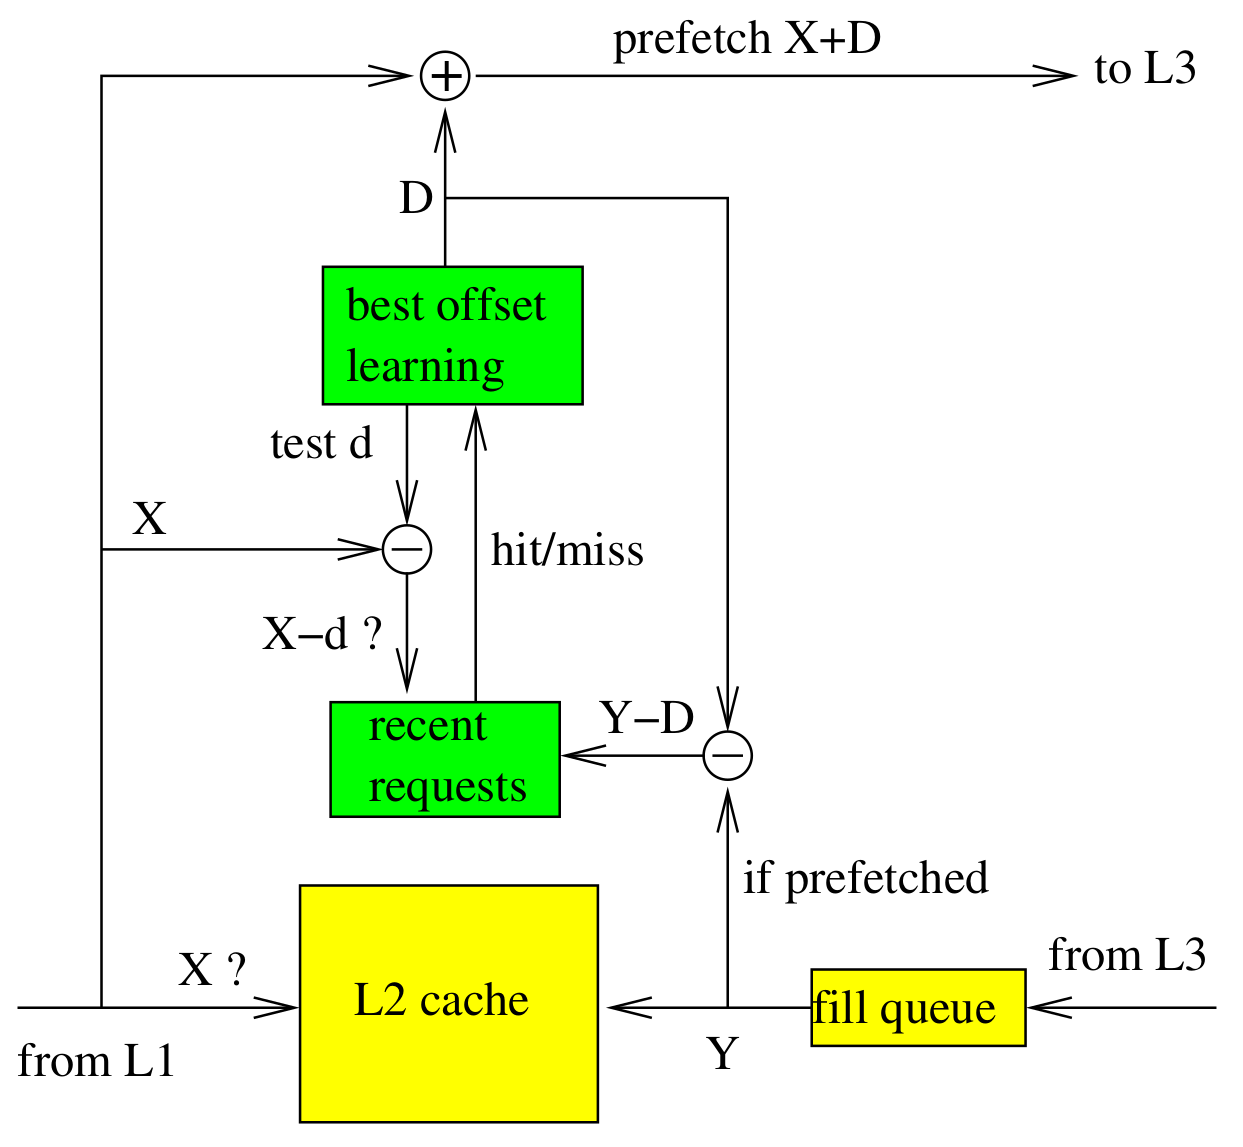
\includegraphics[width=1.0\columnwidth]{figures/michaud_bop_2016_schematic_view_of_bo_prefetcher.png}
    \caption{Schematic view of a BO prefetcher. \cite{BOP_2016}}
    \label{fig:bo-schematic}
\end{figure}


A schematic view of a BO is given in Figure \ref{fig:bo-schematic}.

\subsection{Best-offset learning}

To determine a best offset that may replace the \textit{current} prefetch offset $D$,
the best-offset learning algorithm is employed (Section 4.1 \cite{BOP_2016}): 

"[It] tries to find the best prefetch offset by testing several different offsets.
An offset d is potentially a good prefetch offset if,
when line $X$ is accessed,
there was in the recent past a previous access for line $X - d$.
However, the fact that $X - d$ was recently accessed
is not sufficient for guaranteeing that line $X$ would have been prefetched in time.
We want prefetches to be timely whenever possible.
I.e., for d to be a good prefetch offset for line $X$,
line $X - d$ must have been accessed recently, but not too recently.
Ideally, the time between the accesses to lines $X - d$ and $X$
should be greater than the latency for completing a prefetch request.

\subsection{RR table}

[Michaud's] solution is to record in a \textit{recent requests} (RR) table
the \textit{base address} of prefetch requests that have been \textbf{completed}"\cite{BOP_2016}.

The base address is defined as $Y - D$, where $Y$ is a prefetched line that is ready to be placed in L2 cache.
Vice versa you can think i.e. of a L2 prefetched hit on line $X'$ 20 clock cycles ago.
Then our overall offset prefetcher issues an prefetch for $X' + D$.
Due to L3 latency, this prefetched line $X' + D$ arrives at first after 20 clock cycles in the fill queue from L3.
Then $Y = X' + D$ and the prefeched-bit of that inserted line is set.
Now we know that $Y - D$ must have been a useful for L1 some clock cycles ago (recently).
That's why this base address $X' = Y - D$ is inserted into the recent requests (RR) table.

This late insert implicitly holds information about the L3 latency.

If a line $X - d$ is in the RR table, it implies,
that d would have been an offset that would have prefetched line $X$ in a timely manner.

\subsection{Offset list}

"Besides the RR table, the BO prefetcher features an \textit{offset list} and
a \textit{score} table. The score table associates a score with
every offset in the offset list. The score value is between 0
and SCOREMAX [\dots].

The prefetch offset is updated at the end of every \textit{learning phase}.
A learning phase consists of several \textit{rounds}. At the
start of a learning phase, all the scores are reset to 0.
On every eligible L2 read access (miss or prefetched hit), we test
an offset $d_i$ from the list. If $X - d_i$ hits in the RR table, the
score of offset $d_i$ is incremented.
During a round, each offset in the list is tested once:
we test $d_1$ on the first access in the round,
$d_2$ on the next access, then $d_3$, and so on.
When all the offsets in the list have been tested, the current round is
finished, and a new round begins from offset $d_1$ again."\cite{BOP_2016}


In the appended section \ref{sec:appendix_bo_learning_example} we present two examples, illustrating how the best learning algorithm is scoring good offsets higher.

\subsection{The end of a learning phase}

"The current learning phase finishes at the end of a round
when either of the two following events happens first: one
of the scores equals SCOREMAX, or the number of rounds
equals ROUNDMAX (a fixed parameter). When the learning phase is finished, we search the best offset, i.e., the one
with the highest score3 . This offset becomes the new prefetch
offset, and a new learning phase starts."\cite{BOP_2016}

\subsection{Prefetch throttling}

Prefetching with a fixed offset on very irregular workloads might not be efficient,
with respect to prefetch accuracy. This can result in replacement of useful cache lines.

Therefore the BO prefetcher employes a metric for switching off prefetching.
When no score is above a threshold BADSCORE after a finished learning phase, prefetching is switched off.

But the BO learning proceeds.
Figure \ref{fig:bo-schematic} illustrates the case for prefetching enabled.
But now the tag itself (Y-0) filled into L2 is always added to RR table - not just if it is a prefetched fill.


\section{Implementation: Our Best-Offset Prefetcher}
%explain implementation details so others can reproduce the prefetcher
%good figures can be valuable! (block diagram, state machine/ transistions...)

\subsection{Configuration parameters}

We declare several configuration parameters: \texttt{SCORE\_MAX}, \texttt{ROUND\_MAX} and \texttt{BAD\_SCORE}.
In addition we define \texttt{NUMBER\_OF\_OFFSETS} and \texttt{RR\_SIZE}, to be able
to perform simulations with a subset of the offset-list and different RR table sizes.

\subsection{Offset list}

The authors of the paper \cite{BOP_2016} use a list of prefetch offsets between 1 and 256, where $d \in \{2^i*3^j*5^k\}$.
The BO prefetcher is not prefetching accross page boundaries. Our system has 64B cache lines and we assume 4KiB pages.
But according to the paper the BO prefetcher does not prefetch across page boundaries.
Therefore we limit the offsets to be smaller than 64.
Then our offset list consists of 26 entries:
1,2,3,4,
5,6,8,9,
10,12,15,16,
18,20,24,25,
27,30,32,36,
40,45,48,50,
54,60.

\subsection{Internal State}
First of all the internal state consists of the currently used \texttt{bestOffset} for prefetching.

The paper states that several implementations of the \textit{RR table} are possible.
For the sake of simplicity we decided against modelling a direct-mapped like cache, accessed through a hash function, as proposed by the paper.
Instead we imitate a simple ring buffer, by using a double-ended queue (\texttt{std::deque} of \texttt{int}), to implement the recent requests list.


Furthermore a \textit{flag} that is indicating whether prefetching is \textit{enabled} and
counters for the \texttt{round} and
the \texttt{subround}. The latter one is corresponding to $i$ pointing to the offset $d_i$ to be tested on one eligible L2 access and is incremented on every access.
The \texttt{subround} counter is beeing reset when it is equal to \texttt{NUMBER\_OF\_OFFSETS}.
The \texttt{round} counter is reset when the end of a learning phase is reached. (See section Best Offset Learning).


\subsection{Functions}

Our implementation derives from the gem5 \texttt{Queued : Base} prefetcher.

In order to model the tagged prefetching behaviour and making sure the method \texttt{calculatePrefetch} is beeing invoked only on L2 read accesses that are misses or prefetched hits,
we set the \texttt{Base} prefetcher parameters
\texttt{on\_miss}, \texttt{on\_read}, \texttt{on\_data}, \texttt{on\_inst} and \texttt{prefetch\_on\_pf\_hit}) to \textit{true},
and \texttt{on\_write} and \texttt{prefetch\_on\_access} to \textit{false}.

We also implement methods \texttt{notifyFill} and \texttt{notifyPrefetchFill} that are beeing invoked
when a cache line from L3 is filled into L2 cache, the latter one only when the line has been prefetched. This is required by the scheme (see figure \ref{fig:bo-schematic}).

The implementation of the event listener for \texttt{notifyPrefetchFill} has been provided by our teachers. (https://github.com/davidmetz/gem5-tdt4260/tree/student)

\subsection{Ressource usage}

The BO prefetcher generally has a small hardware overhead \cite{BOP_2016}.
In addition to the (very small) offset prefetching overhead,
just a bit of bookkeeping for recent requests and scores is required.
%For example it does not require an extra prefetch buffer, but prefetched lines as well as demand misses are placed (via the MSHR buffer) directly into the L2 cache.

However for the sake of a readable implementation we use software data structures that were not meaningfully directly implemented in hardware, for example the \texttt{deque} and the \texttt{vector}.
Instead the RR table might be represented for example by a little cache providing hits or misses and indexed by a hash function \cite{BOP_2016}. This reduces memory usage significantly in contrast to saving the pure full addresses.
Also the offset list might be hard-coded in read only memory (ROM).

\subsection{Environment}

We made only few adjustments to the provided baseline architecture configuration of gem5. It has been provided to us by our teachers.\footnote{available under https://github.com/davidmetz/gem5-tdt4260/tree/student}
It comes with a single out-of-order O3 CPU. The system is modelled according to parameters published by Intel in their "Register file prefetching" paper \cite{intel_register_file_prefetching} to match an Intel Ice Lake CPU.
The L1 data cache size is 48KiB, associativity 12; L1 instruction cache size is 32KiB; L2 cache size is 1280KiB, associativity 20; and L3 cache size is 3MiB, associativity 12.
The cache line size is 64B.

We disable hardware prefetching except for the L2 cache, where we employ our Best Offset prefetcher.

\section{Methodology}
%Is a methodology recognizable? Which ones were used? How were the results obtained and analyzed? Are they reproducible? What is the significance and are their possible problems or error sources?

We want to find the best performing configuration of BO parameters on our system for a given workload.

We measure performance by instructions per cycle (IPC), accuracy\footnote{Measures the number of useful prefetches issued by the prefetcher.} and
coverage.\footnote{How many of the potential candidates for prefetches were actually identified by the prefetcher?}.
All these performance parameters are being generated automatically on a run of the provided \texttt{run\_prefetcher.py} script.

Due to time constraints we limit our search on three changed parameters and only one benchmark.

We utilise the provided SPEC2017 gcc\_s benchmark\cite{spec2017gccs}.
The prefetcher is employed and the statistics are being generated after some warm-up of the benchmark.
The number of instructions executed by the simulator is limited to $10\,\text{million}$.

In accordance to \cite[table 2]{BOP_2016} we keep following parameters fixed: $\texttt{ROUND\_MAX} = 100$ and $\texttt{BAD\_SCORE} = 1$.
But we change simulate over differing RR table size, offsets and \texttt{SOCRE\_MAX}:
\begin{itemize}
    \item $\texttt{RR\_SIZE} = \{16, 32, 64, 128, 256\}$
    \item a subset (just the first 16 entries) and the full offset list\footnote{$\texttt{NUMBER\_OF\_OFFSETS} = \{16, 26\}$}
    \item $\texttt{SCORE\_MAX} = \{1,2,\dots,100\}$
\end{itemize}
This gives a total of $2 * 5 * 100 = 1000\,\text{simulations}$.


%testing-scheme: which simulations and what benchmarks and why?
%which peformance metrics to choose (accuracy, coverage, speed, ...)


\section{Results}
%How extensive was the benchmarking? Were different parameters or implementations used? Were there tests of other than already provided benchmarks (optional!)? Are the results well presented (figures, tables)?

\begin{table}
    \centering
    \begin{tabular}{|l|>{\raggedright\arraybackslash}p{0.13\columnwidth}|>{\raggedright\arraybackslash}p{0.13\linewidth}|>{\raggedright\arraybackslash}p{0.13\linewidth}|>{\raggedright\arraybackslash}p{0.13\linewidth}|} \hline 
                  & No Prefetcher  & Tagged Next-Line & BO Maximise IPC     & BO Maximise Accuracy \\ \hline %& BO Maximise Coverage \\ \hline 
         IPC      & 0.236531       & 0.441386         & \textbf{0.577577}   & 0.522890             \\ \hline %& 0.576559             \\ \hline 
         Speedup  & 1.000000       & 1.866081         & \textbf{2.441866}   & 2.210662             \\ \hline %& 2.437562             \\ \hline 
         Accuracy & n/a            & 0.366883         & 0.899859            & \textbf{0.920615}    \\ \hline %& 0.910683             \\ \hline 
         Coverage & n/a            & 0.901658         & 0.715169            & 0.670101             \\ \hline %& \textbf{0.715780}    \\ \hline
         \texttt{RR\_SIZE}   & n/a & n/a              & 16                  & 64                   \\ \hline %& 16                   \\ \hline
         \texttt{SCORE\_MAX} & n/a & n/a              & 7                   & 55                   \\ \hline %& 10                   \\ \hline
         Offsets  & n/a            & n/a              & all 26              & just 16              \\ \hline %& all 26               \\ \hline
    \end{tabular}
    \caption{Comparison of the best performing BO prefetcher configurations against a reference with no prefetching and simple next-line prefetching. Benchmark: gcc\_s, $\texttt{ROUND\_MAX} = 100$ and $\texttt{BAD\_SCORE} = 1$}
    \label{tab:best_parameters}
\end{table}
% REFERENCE-NO-PREFECHING:
% IPC: 0.236531
% Accuracy: n/a
% Coverage: n/a
% REFERENCE-TAGGED-NEXT-LINE-PF:
% IPC: 0.441386
% Accuracy: 0.366883
% Coverage: 0.901658
% BEST-OFFSET:
% -----
% Best IPC: 0.577577
% Accuracy: 0.899859
% Coverage: 0.715169
% Scoremax: 7
% Folder:   RR16offsets26
% -----
% IPC:           0.522890
% Best accuracy: 0.920615
% Coverage:      0.670101
% Scoremax: 55
% Folder:   RR64offsets16
% -----
% IPC:           0.576559
% Accuracy:      0.910683
% Best coverage: 0.715780
% Scoremax: 10
% Folder:   RR16offsets26
% -----
% Best product: 0.65408147232
% IPC:          0.574317
% Accuracy:     0.91536
% Coverage:     0.714562
% Scoremax: 14
% Folder:   RR16offsets26

Table \ref{tab:best_parameters} presents the best performing configurations found with the simulations.
Additionally we make some interesting observations.

Coverage and IPC are strongly correlated as you can see in figure \ref{fig:accuracy_coverage_ipc_full_offset_list_rr_16_32_64}.
Therefore we omit a column showing the results for maximising coverage as they are very similar to those for maximising IPC.

Optimising for IPC, accuracy or coverage may result in quite different BO parameters.
BO can easily outperform next-line with respect to IPC and accuracy but not with respect to coverage.

When maximising accuracy we encounter a more worse IPC. A bigger RR table and the smaller offset subset are beneficial for accuracy.

When maximising IPC we encounter $1.2\,\%$ late prefetches  in contrast to when maximising for accuracy, where we encounter just $0.6\,\%$ late prefetches.
This confirms Michaud's statement that striving for timeliness may not always be optimal\cite[section 2.3]{BOP_2015}.

Generally increasing \texttt{SCORE\_MAX} is beneficial for performance except for either small RR tables sizes (see figure \ref{subfig:RR=16_offsets=26}) or less number of offsets (see figure \ref{subfig:RR=64_Coverage}, blue line).

%TODO: what is the best performing config with respect to IPC, accuracy and coverage -> table

We also saw that using a smaller set of offsets is very beneficial.
See figure \ref{fig:comparision_different_offsets} where for a sufficiently large RR table size and the small offset set ($\leq 25$), any chosen \texttt{SCORE\_MAX} is outperforming the full set of offsets ($\leq 60$).
This may be caused firstly by smaller offsets generally being beneficial for performance (ignoring timeliness) and secondly by the relatively high \texttt{ROUND\_MAX} parameter. With less number of offsets the prefetcher might become more flexible on changing request patterns because learning phases become shorter.

It turned out that performance for RR tables larger than 64 entries is stays quite similar or is even degrading.
We omit related figures.
The degrading effect may come from the BO algorithm wrongly scoring offsets that only satisfy \textit{out-dated} request patterns.
Therefore the RR table should be choosen not too large\cite[section 3.1]{Multi-Lookahead}.


\begin{figure}
     \centering
     \begin{subfigure}[b]{1.0\columnwidth}
         \centering
         %\includegraphics[width=\columnwidth]{graph1}
         \resizebox{1.0\columnwidth}{!}{%% Creator: Matplotlib, PGF backend
%%
%% To include the figure in your LaTeX document, write
%%   \input{<filename>.pgf}
%%
%% Make sure the required packages are loaded in your preamble
%%   \usepackage{pgf}
%%
%% Also ensure that all the required font packages are loaded; for instance,
%% the lmodern package is sometimes necessary when using math font.
%%   \usepackage{lmodern}
%%
%% Figures using additional raster images can only be included by \input if
%% they are in the same directory as the main LaTeX file. For loading figures
%% from other directories you can use the `import` package
%%   \usepackage{import}
%%
%% and then include the figures with
%%   \import{<path to file>}{<filename>.pgf}
%%
%% Matplotlib used the following preamble
%%   \def\mathdefault#1{#1}
%%   \everymath=\expandafter{\the\everymath\displaystyle}
%%   
%%   \makeatletter\@ifpackageloaded{underscore}{}{\usepackage[strings]{underscore}}\makeatother
%%
\begingroup%
\makeatletter%
\begin{pgfpicture}%
\pgfpathrectangle{\pgfpointorigin}{\pgfqpoint{6.400000in}{4.800000in}}%
\pgfusepath{use as bounding box, clip}%
\begin{pgfscope}%
\pgfsetbuttcap%
\pgfsetmiterjoin%
\definecolor{currentfill}{rgb}{1.000000,1.000000,1.000000}%
\pgfsetfillcolor{currentfill}%
\pgfsetlinewidth{0.000000pt}%
\definecolor{currentstroke}{rgb}{1.000000,1.000000,1.000000}%
\pgfsetstrokecolor{currentstroke}%
\pgfsetdash{}{0pt}%
\pgfpathmoveto{\pgfqpoint{0.000000in}{0.000000in}}%
\pgfpathlineto{\pgfqpoint{6.400000in}{0.000000in}}%
\pgfpathlineto{\pgfqpoint{6.400000in}{4.800000in}}%
\pgfpathlineto{\pgfqpoint{0.000000in}{4.800000in}}%
\pgfpathlineto{\pgfqpoint{0.000000in}{0.000000in}}%
\pgfpathclose%
\pgfusepath{fill}%
\end{pgfscope}%
\begin{pgfscope}%
\pgfsetbuttcap%
\pgfsetmiterjoin%
\definecolor{currentfill}{rgb}{1.000000,1.000000,1.000000}%
\pgfsetfillcolor{currentfill}%
\pgfsetlinewidth{0.000000pt}%
\definecolor{currentstroke}{rgb}{0.000000,0.000000,0.000000}%
\pgfsetstrokecolor{currentstroke}%
\pgfsetstrokeopacity{0.000000}%
\pgfsetdash{}{0pt}%
\pgfpathmoveto{\pgfqpoint{0.800000in}{0.528000in}}%
\pgfpathlineto{\pgfqpoint{5.760000in}{0.528000in}}%
\pgfpathlineto{\pgfqpoint{5.760000in}{4.224000in}}%
\pgfpathlineto{\pgfqpoint{0.800000in}{4.224000in}}%
\pgfpathlineto{\pgfqpoint{0.800000in}{0.528000in}}%
\pgfpathclose%
\pgfusepath{fill}%
\end{pgfscope}%
\begin{pgfscope}%
\pgfpathrectangle{\pgfqpoint{0.800000in}{0.528000in}}{\pgfqpoint{4.960000in}{3.696000in}}%
\pgfusepath{clip}%
\pgfsetbuttcap%
\pgfsetroundjoin%
\pgfsetlinewidth{0.803000pt}%
\definecolor{currentstroke}{rgb}{0.000000,0.000000,0.000000}%
\pgfsetstrokecolor{currentstroke}%
\pgfsetstrokeopacity{0.500000}%
\pgfsetdash{{0.800000pt}{1.320000pt}}{0.000000pt}%
\pgfpathmoveto{\pgfqpoint{0.953882in}{0.528000in}}%
\pgfpathlineto{\pgfqpoint{0.953882in}{4.224000in}}%
\pgfusepath{stroke}%
\end{pgfscope}%
\begin{pgfscope}%
\pgfsetbuttcap%
\pgfsetroundjoin%
\definecolor{currentfill}{rgb}{0.000000,0.000000,0.000000}%
\pgfsetfillcolor{currentfill}%
\pgfsetlinewidth{0.803000pt}%
\definecolor{currentstroke}{rgb}{0.000000,0.000000,0.000000}%
\pgfsetstrokecolor{currentstroke}%
\pgfsetdash{}{0pt}%
\pgfsys@defobject{currentmarker}{\pgfqpoint{0.000000in}{-0.048611in}}{\pgfqpoint{0.000000in}{0.000000in}}{%
\pgfpathmoveto{\pgfqpoint{0.000000in}{0.000000in}}%
\pgfpathlineto{\pgfqpoint{0.000000in}{-0.048611in}}%
\pgfusepath{stroke,fill}%
}%
\begin{pgfscope}%
\pgfsys@transformshift{0.953882in}{0.528000in}%
\pgfsys@useobject{currentmarker}{}%
\end{pgfscope}%
\end{pgfscope}%
\begin{pgfscope}%
\definecolor{textcolor}{rgb}{0.000000,0.000000,0.000000}%
\pgfsetstrokecolor{textcolor}%
\pgfsetfillcolor{textcolor}%
\pgftext[x=0.953882in,y=0.430778in,,top]{\color{textcolor}{\sffamily\fontsize{10.000000}{12.000000}\selectfont\catcode`\^=\active\def^{\ifmmode\sp\else\^{}\fi}\catcode`\%=\active\def%{\%}0}}%
\end{pgfscope}%
\begin{pgfscope}%
\pgfpathrectangle{\pgfqpoint{0.800000in}{0.528000in}}{\pgfqpoint{4.960000in}{3.696000in}}%
\pgfusepath{clip}%
\pgfsetbuttcap%
\pgfsetroundjoin%
\pgfsetlinewidth{0.803000pt}%
\definecolor{currentstroke}{rgb}{0.000000,0.000000,0.000000}%
\pgfsetstrokecolor{currentstroke}%
\pgfsetstrokeopacity{0.500000}%
\pgfsetdash{{0.800000pt}{1.320000pt}}{0.000000pt}%
\pgfpathmoveto{\pgfqpoint{1.669610in}{0.528000in}}%
\pgfpathlineto{\pgfqpoint{1.669610in}{4.224000in}}%
\pgfusepath{stroke}%
\end{pgfscope}%
\begin{pgfscope}%
\pgfsetbuttcap%
\pgfsetroundjoin%
\definecolor{currentfill}{rgb}{0.000000,0.000000,0.000000}%
\pgfsetfillcolor{currentfill}%
\pgfsetlinewidth{0.803000pt}%
\definecolor{currentstroke}{rgb}{0.000000,0.000000,0.000000}%
\pgfsetstrokecolor{currentstroke}%
\pgfsetdash{}{0pt}%
\pgfsys@defobject{currentmarker}{\pgfqpoint{0.000000in}{-0.048611in}}{\pgfqpoint{0.000000in}{0.000000in}}{%
\pgfpathmoveto{\pgfqpoint{0.000000in}{0.000000in}}%
\pgfpathlineto{\pgfqpoint{0.000000in}{-0.048611in}}%
\pgfusepath{stroke,fill}%
}%
\begin{pgfscope}%
\pgfsys@transformshift{1.669610in}{0.528000in}%
\pgfsys@useobject{currentmarker}{}%
\end{pgfscope}%
\end{pgfscope}%
\begin{pgfscope}%
\definecolor{textcolor}{rgb}{0.000000,0.000000,0.000000}%
\pgfsetstrokecolor{textcolor}%
\pgfsetfillcolor{textcolor}%
\pgftext[x=1.669610in,y=0.430778in,,top]{\color{textcolor}{\sffamily\fontsize{10.000000}{12.000000}\selectfont\catcode`\^=\active\def^{\ifmmode\sp\else\^{}\fi}\catcode`\%=\active\def%{\%}10}}%
\end{pgfscope}%
\begin{pgfscope}%
\pgfpathrectangle{\pgfqpoint{0.800000in}{0.528000in}}{\pgfqpoint{4.960000in}{3.696000in}}%
\pgfusepath{clip}%
\pgfsetbuttcap%
\pgfsetroundjoin%
\pgfsetlinewidth{0.803000pt}%
\definecolor{currentstroke}{rgb}{0.000000,0.000000,0.000000}%
\pgfsetstrokecolor{currentstroke}%
\pgfsetstrokeopacity{0.500000}%
\pgfsetdash{{0.800000pt}{1.320000pt}}{0.000000pt}%
\pgfpathmoveto{\pgfqpoint{2.385339in}{0.528000in}}%
\pgfpathlineto{\pgfqpoint{2.385339in}{4.224000in}}%
\pgfusepath{stroke}%
\end{pgfscope}%
\begin{pgfscope}%
\pgfsetbuttcap%
\pgfsetroundjoin%
\definecolor{currentfill}{rgb}{0.000000,0.000000,0.000000}%
\pgfsetfillcolor{currentfill}%
\pgfsetlinewidth{0.803000pt}%
\definecolor{currentstroke}{rgb}{0.000000,0.000000,0.000000}%
\pgfsetstrokecolor{currentstroke}%
\pgfsetdash{}{0pt}%
\pgfsys@defobject{currentmarker}{\pgfqpoint{0.000000in}{-0.048611in}}{\pgfqpoint{0.000000in}{0.000000in}}{%
\pgfpathmoveto{\pgfqpoint{0.000000in}{0.000000in}}%
\pgfpathlineto{\pgfqpoint{0.000000in}{-0.048611in}}%
\pgfusepath{stroke,fill}%
}%
\begin{pgfscope}%
\pgfsys@transformshift{2.385339in}{0.528000in}%
\pgfsys@useobject{currentmarker}{}%
\end{pgfscope}%
\end{pgfscope}%
\begin{pgfscope}%
\definecolor{textcolor}{rgb}{0.000000,0.000000,0.000000}%
\pgfsetstrokecolor{textcolor}%
\pgfsetfillcolor{textcolor}%
\pgftext[x=2.385339in,y=0.430778in,,top]{\color{textcolor}{\sffamily\fontsize{10.000000}{12.000000}\selectfont\catcode`\^=\active\def^{\ifmmode\sp\else\^{}\fi}\catcode`\%=\active\def%{\%}20}}%
\end{pgfscope}%
\begin{pgfscope}%
\pgfpathrectangle{\pgfqpoint{0.800000in}{0.528000in}}{\pgfqpoint{4.960000in}{3.696000in}}%
\pgfusepath{clip}%
\pgfsetbuttcap%
\pgfsetroundjoin%
\pgfsetlinewidth{0.803000pt}%
\definecolor{currentstroke}{rgb}{0.000000,0.000000,0.000000}%
\pgfsetstrokecolor{currentstroke}%
\pgfsetstrokeopacity{0.500000}%
\pgfsetdash{{0.800000pt}{1.320000pt}}{0.000000pt}%
\pgfpathmoveto{\pgfqpoint{3.101068in}{0.528000in}}%
\pgfpathlineto{\pgfqpoint{3.101068in}{4.224000in}}%
\pgfusepath{stroke}%
\end{pgfscope}%
\begin{pgfscope}%
\pgfsetbuttcap%
\pgfsetroundjoin%
\definecolor{currentfill}{rgb}{0.000000,0.000000,0.000000}%
\pgfsetfillcolor{currentfill}%
\pgfsetlinewidth{0.803000pt}%
\definecolor{currentstroke}{rgb}{0.000000,0.000000,0.000000}%
\pgfsetstrokecolor{currentstroke}%
\pgfsetdash{}{0pt}%
\pgfsys@defobject{currentmarker}{\pgfqpoint{0.000000in}{-0.048611in}}{\pgfqpoint{0.000000in}{0.000000in}}{%
\pgfpathmoveto{\pgfqpoint{0.000000in}{0.000000in}}%
\pgfpathlineto{\pgfqpoint{0.000000in}{-0.048611in}}%
\pgfusepath{stroke,fill}%
}%
\begin{pgfscope}%
\pgfsys@transformshift{3.101068in}{0.528000in}%
\pgfsys@useobject{currentmarker}{}%
\end{pgfscope}%
\end{pgfscope}%
\begin{pgfscope}%
\definecolor{textcolor}{rgb}{0.000000,0.000000,0.000000}%
\pgfsetstrokecolor{textcolor}%
\pgfsetfillcolor{textcolor}%
\pgftext[x=3.101068in,y=0.430778in,,top]{\color{textcolor}{\sffamily\fontsize{10.000000}{12.000000}\selectfont\catcode`\^=\active\def^{\ifmmode\sp\else\^{}\fi}\catcode`\%=\active\def%{\%}30}}%
\end{pgfscope}%
\begin{pgfscope}%
\pgfpathrectangle{\pgfqpoint{0.800000in}{0.528000in}}{\pgfqpoint{4.960000in}{3.696000in}}%
\pgfusepath{clip}%
\pgfsetbuttcap%
\pgfsetroundjoin%
\pgfsetlinewidth{0.803000pt}%
\definecolor{currentstroke}{rgb}{0.000000,0.000000,0.000000}%
\pgfsetstrokecolor{currentstroke}%
\pgfsetstrokeopacity{0.500000}%
\pgfsetdash{{0.800000pt}{1.320000pt}}{0.000000pt}%
\pgfpathmoveto{\pgfqpoint{3.816797in}{0.528000in}}%
\pgfpathlineto{\pgfqpoint{3.816797in}{4.224000in}}%
\pgfusepath{stroke}%
\end{pgfscope}%
\begin{pgfscope}%
\pgfsetbuttcap%
\pgfsetroundjoin%
\definecolor{currentfill}{rgb}{0.000000,0.000000,0.000000}%
\pgfsetfillcolor{currentfill}%
\pgfsetlinewidth{0.803000pt}%
\definecolor{currentstroke}{rgb}{0.000000,0.000000,0.000000}%
\pgfsetstrokecolor{currentstroke}%
\pgfsetdash{}{0pt}%
\pgfsys@defobject{currentmarker}{\pgfqpoint{0.000000in}{-0.048611in}}{\pgfqpoint{0.000000in}{0.000000in}}{%
\pgfpathmoveto{\pgfqpoint{0.000000in}{0.000000in}}%
\pgfpathlineto{\pgfqpoint{0.000000in}{-0.048611in}}%
\pgfusepath{stroke,fill}%
}%
\begin{pgfscope}%
\pgfsys@transformshift{3.816797in}{0.528000in}%
\pgfsys@useobject{currentmarker}{}%
\end{pgfscope}%
\end{pgfscope}%
\begin{pgfscope}%
\definecolor{textcolor}{rgb}{0.000000,0.000000,0.000000}%
\pgfsetstrokecolor{textcolor}%
\pgfsetfillcolor{textcolor}%
\pgftext[x=3.816797in,y=0.430778in,,top]{\color{textcolor}{\sffamily\fontsize{10.000000}{12.000000}\selectfont\catcode`\^=\active\def^{\ifmmode\sp\else\^{}\fi}\catcode`\%=\active\def%{\%}40}}%
\end{pgfscope}%
\begin{pgfscope}%
\pgfpathrectangle{\pgfqpoint{0.800000in}{0.528000in}}{\pgfqpoint{4.960000in}{3.696000in}}%
\pgfusepath{clip}%
\pgfsetbuttcap%
\pgfsetroundjoin%
\pgfsetlinewidth{0.803000pt}%
\definecolor{currentstroke}{rgb}{0.000000,0.000000,0.000000}%
\pgfsetstrokecolor{currentstroke}%
\pgfsetstrokeopacity{0.500000}%
\pgfsetdash{{0.800000pt}{1.320000pt}}{0.000000pt}%
\pgfpathmoveto{\pgfqpoint{4.532525in}{0.528000in}}%
\pgfpathlineto{\pgfqpoint{4.532525in}{4.224000in}}%
\pgfusepath{stroke}%
\end{pgfscope}%
\begin{pgfscope}%
\pgfsetbuttcap%
\pgfsetroundjoin%
\definecolor{currentfill}{rgb}{0.000000,0.000000,0.000000}%
\pgfsetfillcolor{currentfill}%
\pgfsetlinewidth{0.803000pt}%
\definecolor{currentstroke}{rgb}{0.000000,0.000000,0.000000}%
\pgfsetstrokecolor{currentstroke}%
\pgfsetdash{}{0pt}%
\pgfsys@defobject{currentmarker}{\pgfqpoint{0.000000in}{-0.048611in}}{\pgfqpoint{0.000000in}{0.000000in}}{%
\pgfpathmoveto{\pgfqpoint{0.000000in}{0.000000in}}%
\pgfpathlineto{\pgfqpoint{0.000000in}{-0.048611in}}%
\pgfusepath{stroke,fill}%
}%
\begin{pgfscope}%
\pgfsys@transformshift{4.532525in}{0.528000in}%
\pgfsys@useobject{currentmarker}{}%
\end{pgfscope}%
\end{pgfscope}%
\begin{pgfscope}%
\definecolor{textcolor}{rgb}{0.000000,0.000000,0.000000}%
\pgfsetstrokecolor{textcolor}%
\pgfsetfillcolor{textcolor}%
\pgftext[x=4.532525in,y=0.430778in,,top]{\color{textcolor}{\sffamily\fontsize{10.000000}{12.000000}\selectfont\catcode`\^=\active\def^{\ifmmode\sp\else\^{}\fi}\catcode`\%=\active\def%{\%}50}}%
\end{pgfscope}%
\begin{pgfscope}%
\pgfpathrectangle{\pgfqpoint{0.800000in}{0.528000in}}{\pgfqpoint{4.960000in}{3.696000in}}%
\pgfusepath{clip}%
\pgfsetbuttcap%
\pgfsetroundjoin%
\pgfsetlinewidth{0.803000pt}%
\definecolor{currentstroke}{rgb}{0.000000,0.000000,0.000000}%
\pgfsetstrokecolor{currentstroke}%
\pgfsetstrokeopacity{0.500000}%
\pgfsetdash{{0.800000pt}{1.320000pt}}{0.000000pt}%
\pgfpathmoveto{\pgfqpoint{5.248254in}{0.528000in}}%
\pgfpathlineto{\pgfqpoint{5.248254in}{4.224000in}}%
\pgfusepath{stroke}%
\end{pgfscope}%
\begin{pgfscope}%
\pgfsetbuttcap%
\pgfsetroundjoin%
\definecolor{currentfill}{rgb}{0.000000,0.000000,0.000000}%
\pgfsetfillcolor{currentfill}%
\pgfsetlinewidth{0.803000pt}%
\definecolor{currentstroke}{rgb}{0.000000,0.000000,0.000000}%
\pgfsetstrokecolor{currentstroke}%
\pgfsetdash{}{0pt}%
\pgfsys@defobject{currentmarker}{\pgfqpoint{0.000000in}{-0.048611in}}{\pgfqpoint{0.000000in}{0.000000in}}{%
\pgfpathmoveto{\pgfqpoint{0.000000in}{0.000000in}}%
\pgfpathlineto{\pgfqpoint{0.000000in}{-0.048611in}}%
\pgfusepath{stroke,fill}%
}%
\begin{pgfscope}%
\pgfsys@transformshift{5.248254in}{0.528000in}%
\pgfsys@useobject{currentmarker}{}%
\end{pgfscope}%
\end{pgfscope}%
\begin{pgfscope}%
\definecolor{textcolor}{rgb}{0.000000,0.000000,0.000000}%
\pgfsetstrokecolor{textcolor}%
\pgfsetfillcolor{textcolor}%
\pgftext[x=5.248254in,y=0.430778in,,top]{\color{textcolor}{\sffamily\fontsize{10.000000}{12.000000}\selectfont\catcode`\^=\active\def^{\ifmmode\sp\else\^{}\fi}\catcode`\%=\active\def%{\%}60}}%
\end{pgfscope}%
\begin{pgfscope}%
\definecolor{textcolor}{rgb}{0.000000,0.000000,0.000000}%
\pgfsetstrokecolor{textcolor}%
\pgfsetfillcolor{textcolor}%
\pgftext[x=3.280000in,y=0.251766in,,top]{\color{textcolor}{\sffamily\fontsize{10.000000}{12.000000}\selectfont\catcode`\^=\active\def^{\ifmmode\sp\else\^{}\fi}\catcode`\%=\active\def%{\%}\texttt{SCORE\_MAX}}}%
\end{pgfscope}%
\begin{pgfscope}%
\pgfpathrectangle{\pgfqpoint{0.800000in}{0.528000in}}{\pgfqpoint{4.960000in}{3.696000in}}%
\pgfusepath{clip}%
\pgfsetbuttcap%
\pgfsetroundjoin%
\pgfsetlinewidth{0.803000pt}%
\definecolor{currentstroke}{rgb}{0.000000,0.000000,0.000000}%
\pgfsetstrokecolor{currentstroke}%
\pgfsetstrokeopacity{0.500000}%
\pgfsetdash{{0.800000pt}{1.320000pt}}{0.000000pt}%
\pgfpathmoveto{\pgfqpoint{0.800000in}{0.662052in}}%
\pgfpathlineto{\pgfqpoint{5.760000in}{0.662052in}}%
\pgfusepath{stroke}%
\end{pgfscope}%
\begin{pgfscope}%
\pgfsetbuttcap%
\pgfsetroundjoin%
\definecolor{currentfill}{rgb}{0.000000,0.000000,0.000000}%
\pgfsetfillcolor{currentfill}%
\pgfsetlinewidth{0.803000pt}%
\definecolor{currentstroke}{rgb}{0.000000,0.000000,0.000000}%
\pgfsetstrokecolor{currentstroke}%
\pgfsetdash{}{0pt}%
\pgfsys@defobject{currentmarker}{\pgfqpoint{-0.048611in}{0.000000in}}{\pgfqpoint{-0.000000in}{0.000000in}}{%
\pgfpathmoveto{\pgfqpoint{-0.000000in}{0.000000in}}%
\pgfpathlineto{\pgfqpoint{-0.048611in}{0.000000in}}%
\pgfusepath{stroke,fill}%
}%
\begin{pgfscope}%
\pgfsys@transformshift{0.800000in}{0.662052in}%
\pgfsys@useobject{currentmarker}{}%
\end{pgfscope}%
\end{pgfscope}%
\begin{pgfscope}%
\definecolor{textcolor}{rgb}{0.000000,0.000000,0.000000}%
\pgfsetstrokecolor{textcolor}%
\pgfsetfillcolor{textcolor}%
\pgftext[x=0.525308in, y=0.613826in, left, base]{\color{textcolor}{\sffamily\fontsize{10.000000}{12.000000}\selectfont\catcode`\^=\active\def^{\ifmmode\sp\else\^{}\fi}\catcode`\%=\active\def%{\%}0.4}}%
\end{pgfscope}%
\begin{pgfscope}%
\pgfpathrectangle{\pgfqpoint{0.800000in}{0.528000in}}{\pgfqpoint{4.960000in}{3.696000in}}%
\pgfusepath{clip}%
\pgfsetbuttcap%
\pgfsetroundjoin%
\pgfsetlinewidth{0.803000pt}%
\definecolor{currentstroke}{rgb}{0.000000,0.000000,0.000000}%
\pgfsetstrokecolor{currentstroke}%
\pgfsetstrokeopacity{0.500000}%
\pgfsetdash{{0.800000pt}{1.320000pt}}{0.000000pt}%
\pgfpathmoveto{\pgfqpoint{0.800000in}{1.314656in}}%
\pgfpathlineto{\pgfqpoint{5.760000in}{1.314656in}}%
\pgfusepath{stroke}%
\end{pgfscope}%
\begin{pgfscope}%
\pgfsetbuttcap%
\pgfsetroundjoin%
\definecolor{currentfill}{rgb}{0.000000,0.000000,0.000000}%
\pgfsetfillcolor{currentfill}%
\pgfsetlinewidth{0.803000pt}%
\definecolor{currentstroke}{rgb}{0.000000,0.000000,0.000000}%
\pgfsetstrokecolor{currentstroke}%
\pgfsetdash{}{0pt}%
\pgfsys@defobject{currentmarker}{\pgfqpoint{-0.048611in}{0.000000in}}{\pgfqpoint{-0.000000in}{0.000000in}}{%
\pgfpathmoveto{\pgfqpoint{-0.000000in}{0.000000in}}%
\pgfpathlineto{\pgfqpoint{-0.048611in}{0.000000in}}%
\pgfusepath{stroke,fill}%
}%
\begin{pgfscope}%
\pgfsys@transformshift{0.800000in}{1.314656in}%
\pgfsys@useobject{currentmarker}{}%
\end{pgfscope}%
\end{pgfscope}%
\begin{pgfscope}%
\definecolor{textcolor}{rgb}{0.000000,0.000000,0.000000}%
\pgfsetstrokecolor{textcolor}%
\pgfsetfillcolor{textcolor}%
\pgftext[x=0.525308in, y=1.266431in, left, base]{\color{textcolor}{\sffamily\fontsize{10.000000}{12.000000}\selectfont\catcode`\^=\active\def^{\ifmmode\sp\else\^{}\fi}\catcode`\%=\active\def%{\%}0.5}}%
\end{pgfscope}%
\begin{pgfscope}%
\pgfpathrectangle{\pgfqpoint{0.800000in}{0.528000in}}{\pgfqpoint{4.960000in}{3.696000in}}%
\pgfusepath{clip}%
\pgfsetbuttcap%
\pgfsetroundjoin%
\pgfsetlinewidth{0.803000pt}%
\definecolor{currentstroke}{rgb}{0.000000,0.000000,0.000000}%
\pgfsetstrokecolor{currentstroke}%
\pgfsetstrokeopacity{0.500000}%
\pgfsetdash{{0.800000pt}{1.320000pt}}{0.000000pt}%
\pgfpathmoveto{\pgfqpoint{0.800000in}{1.967261in}}%
\pgfpathlineto{\pgfqpoint{5.760000in}{1.967261in}}%
\pgfusepath{stroke}%
\end{pgfscope}%
\begin{pgfscope}%
\pgfsetbuttcap%
\pgfsetroundjoin%
\definecolor{currentfill}{rgb}{0.000000,0.000000,0.000000}%
\pgfsetfillcolor{currentfill}%
\pgfsetlinewidth{0.803000pt}%
\definecolor{currentstroke}{rgb}{0.000000,0.000000,0.000000}%
\pgfsetstrokecolor{currentstroke}%
\pgfsetdash{}{0pt}%
\pgfsys@defobject{currentmarker}{\pgfqpoint{-0.048611in}{0.000000in}}{\pgfqpoint{-0.000000in}{0.000000in}}{%
\pgfpathmoveto{\pgfqpoint{-0.000000in}{0.000000in}}%
\pgfpathlineto{\pgfqpoint{-0.048611in}{0.000000in}}%
\pgfusepath{stroke,fill}%
}%
\begin{pgfscope}%
\pgfsys@transformshift{0.800000in}{1.967261in}%
\pgfsys@useobject{currentmarker}{}%
\end{pgfscope}%
\end{pgfscope}%
\begin{pgfscope}%
\definecolor{textcolor}{rgb}{0.000000,0.000000,0.000000}%
\pgfsetstrokecolor{textcolor}%
\pgfsetfillcolor{textcolor}%
\pgftext[x=0.525308in, y=1.919035in, left, base]{\color{textcolor}{\sffamily\fontsize{10.000000}{12.000000}\selectfont\catcode`\^=\active\def^{\ifmmode\sp\else\^{}\fi}\catcode`\%=\active\def%{\%}0.6}}%
\end{pgfscope}%
\begin{pgfscope}%
\pgfpathrectangle{\pgfqpoint{0.800000in}{0.528000in}}{\pgfqpoint{4.960000in}{3.696000in}}%
\pgfusepath{clip}%
\pgfsetbuttcap%
\pgfsetroundjoin%
\pgfsetlinewidth{0.803000pt}%
\definecolor{currentstroke}{rgb}{0.000000,0.000000,0.000000}%
\pgfsetstrokecolor{currentstroke}%
\pgfsetstrokeopacity{0.500000}%
\pgfsetdash{{0.800000pt}{1.320000pt}}{0.000000pt}%
\pgfpathmoveto{\pgfqpoint{0.800000in}{2.619865in}}%
\pgfpathlineto{\pgfqpoint{5.760000in}{2.619865in}}%
\pgfusepath{stroke}%
\end{pgfscope}%
\begin{pgfscope}%
\pgfsetbuttcap%
\pgfsetroundjoin%
\definecolor{currentfill}{rgb}{0.000000,0.000000,0.000000}%
\pgfsetfillcolor{currentfill}%
\pgfsetlinewidth{0.803000pt}%
\definecolor{currentstroke}{rgb}{0.000000,0.000000,0.000000}%
\pgfsetstrokecolor{currentstroke}%
\pgfsetdash{}{0pt}%
\pgfsys@defobject{currentmarker}{\pgfqpoint{-0.048611in}{0.000000in}}{\pgfqpoint{-0.000000in}{0.000000in}}{%
\pgfpathmoveto{\pgfqpoint{-0.000000in}{0.000000in}}%
\pgfpathlineto{\pgfqpoint{-0.048611in}{0.000000in}}%
\pgfusepath{stroke,fill}%
}%
\begin{pgfscope}%
\pgfsys@transformshift{0.800000in}{2.619865in}%
\pgfsys@useobject{currentmarker}{}%
\end{pgfscope}%
\end{pgfscope}%
\begin{pgfscope}%
\definecolor{textcolor}{rgb}{0.000000,0.000000,0.000000}%
\pgfsetstrokecolor{textcolor}%
\pgfsetfillcolor{textcolor}%
\pgftext[x=0.525308in, y=2.571640in, left, base]{\color{textcolor}{\sffamily\fontsize{10.000000}{12.000000}\selectfont\catcode`\^=\active\def^{\ifmmode\sp\else\^{}\fi}\catcode`\%=\active\def%{\%}0.7}}%
\end{pgfscope}%
\begin{pgfscope}%
\pgfpathrectangle{\pgfqpoint{0.800000in}{0.528000in}}{\pgfqpoint{4.960000in}{3.696000in}}%
\pgfusepath{clip}%
\pgfsetbuttcap%
\pgfsetroundjoin%
\pgfsetlinewidth{0.803000pt}%
\definecolor{currentstroke}{rgb}{0.000000,0.000000,0.000000}%
\pgfsetstrokecolor{currentstroke}%
\pgfsetstrokeopacity{0.500000}%
\pgfsetdash{{0.800000pt}{1.320000pt}}{0.000000pt}%
\pgfpathmoveto{\pgfqpoint{0.800000in}{3.272470in}}%
\pgfpathlineto{\pgfqpoint{5.760000in}{3.272470in}}%
\pgfusepath{stroke}%
\end{pgfscope}%
\begin{pgfscope}%
\pgfsetbuttcap%
\pgfsetroundjoin%
\definecolor{currentfill}{rgb}{0.000000,0.000000,0.000000}%
\pgfsetfillcolor{currentfill}%
\pgfsetlinewidth{0.803000pt}%
\definecolor{currentstroke}{rgb}{0.000000,0.000000,0.000000}%
\pgfsetstrokecolor{currentstroke}%
\pgfsetdash{}{0pt}%
\pgfsys@defobject{currentmarker}{\pgfqpoint{-0.048611in}{0.000000in}}{\pgfqpoint{-0.000000in}{0.000000in}}{%
\pgfpathmoveto{\pgfqpoint{-0.000000in}{0.000000in}}%
\pgfpathlineto{\pgfqpoint{-0.048611in}{0.000000in}}%
\pgfusepath{stroke,fill}%
}%
\begin{pgfscope}%
\pgfsys@transformshift{0.800000in}{3.272470in}%
\pgfsys@useobject{currentmarker}{}%
\end{pgfscope}%
\end{pgfscope}%
\begin{pgfscope}%
\definecolor{textcolor}{rgb}{0.000000,0.000000,0.000000}%
\pgfsetstrokecolor{textcolor}%
\pgfsetfillcolor{textcolor}%
\pgftext[x=0.525308in, y=3.224245in, left, base]{\color{textcolor}{\sffamily\fontsize{10.000000}{12.000000}\selectfont\catcode`\^=\active\def^{\ifmmode\sp\else\^{}\fi}\catcode`\%=\active\def%{\%}0.8}}%
\end{pgfscope}%
\begin{pgfscope}%
\pgfpathrectangle{\pgfqpoint{0.800000in}{0.528000in}}{\pgfqpoint{4.960000in}{3.696000in}}%
\pgfusepath{clip}%
\pgfsetbuttcap%
\pgfsetroundjoin%
\pgfsetlinewidth{0.803000pt}%
\definecolor{currentstroke}{rgb}{0.000000,0.000000,0.000000}%
\pgfsetstrokecolor{currentstroke}%
\pgfsetstrokeopacity{0.500000}%
\pgfsetdash{{0.800000pt}{1.320000pt}}{0.000000pt}%
\pgfpathmoveto{\pgfqpoint{0.800000in}{3.925074in}}%
\pgfpathlineto{\pgfqpoint{5.760000in}{3.925074in}}%
\pgfusepath{stroke}%
\end{pgfscope}%
\begin{pgfscope}%
\pgfsetbuttcap%
\pgfsetroundjoin%
\definecolor{currentfill}{rgb}{0.000000,0.000000,0.000000}%
\pgfsetfillcolor{currentfill}%
\pgfsetlinewidth{0.803000pt}%
\definecolor{currentstroke}{rgb}{0.000000,0.000000,0.000000}%
\pgfsetstrokecolor{currentstroke}%
\pgfsetdash{}{0pt}%
\pgfsys@defobject{currentmarker}{\pgfqpoint{-0.048611in}{0.000000in}}{\pgfqpoint{-0.000000in}{0.000000in}}{%
\pgfpathmoveto{\pgfqpoint{-0.000000in}{0.000000in}}%
\pgfpathlineto{\pgfqpoint{-0.048611in}{0.000000in}}%
\pgfusepath{stroke,fill}%
}%
\begin{pgfscope}%
\pgfsys@transformshift{0.800000in}{3.925074in}%
\pgfsys@useobject{currentmarker}{}%
\end{pgfscope}%
\end{pgfscope}%
\begin{pgfscope}%
\definecolor{textcolor}{rgb}{0.000000,0.000000,0.000000}%
\pgfsetstrokecolor{textcolor}%
\pgfsetfillcolor{textcolor}%
\pgftext[x=0.525308in, y=3.876849in, left, base]{\color{textcolor}{\sffamily\fontsize{10.000000}{12.000000}\selectfont\catcode`\^=\active\def^{\ifmmode\sp\else\^{}\fi}\catcode`\%=\active\def%{\%}0.9}}%
\end{pgfscope}%
\begin{pgfscope}%
\definecolor{textcolor}{rgb}{0.000000,0.000000,0.000000}%
\pgfsetstrokecolor{textcolor}%
\pgfsetfillcolor{textcolor}%
\pgftext[x=0.469752in,y=2.376000in,,bottom,rotate=90.000000]{\color{textcolor}{\sffamily\fontsize{10.000000}{12.000000}\selectfont\catcode`\^=\active\def^{\ifmmode\sp\else\^{}\fi}\catcode`\%=\active\def%{\%}Accuracy | Coverage | IPC}}%
\end{pgfscope}%
\begin{pgfscope}%
\pgfpathrectangle{\pgfqpoint{0.800000in}{0.528000in}}{\pgfqpoint{4.960000in}{3.696000in}}%
\pgfusepath{clip}%
\pgfsetrectcap%
\pgfsetroundjoin%
\pgfsetlinewidth{1.003750pt}%
\definecolor{currentstroke}{rgb}{0.121569,0.466667,0.705882}%
\pgfsetstrokecolor{currentstroke}%
\pgfsetdash{}{0pt}%
\pgfpathmoveto{\pgfqpoint{1.025455in}{2.737726in}}%
\pgfpathlineto{\pgfqpoint{1.097027in}{3.306059in}}%
\pgfpathlineto{\pgfqpoint{1.168600in}{3.470157in}}%
\pgfpathlineto{\pgfqpoint{1.240173in}{3.705714in}}%
\pgfpathlineto{\pgfqpoint{1.311746in}{3.821232in}}%
\pgfpathlineto{\pgfqpoint{1.383319in}{3.890330in}}%
\pgfpathlineto{\pgfqpoint{1.454892in}{3.924154in}}%
\pgfpathlineto{\pgfqpoint{1.526465in}{3.970280in}}%
\pgfpathlineto{\pgfqpoint{1.598038in}{3.972290in}}%
\pgfpathlineto{\pgfqpoint{1.669610in}{3.994792in}}%
\pgfpathlineto{\pgfqpoint{1.741183in}{3.990452in}}%
\pgfpathlineto{\pgfqpoint{1.812756in}{4.010872in}}%
\pgfpathlineto{\pgfqpoint{1.884329in}{4.011179in}}%
\pgfpathlineto{\pgfqpoint{1.955902in}{4.025315in}}%
\pgfpathlineto{\pgfqpoint{2.027475in}{4.015630in}}%
\pgfpathlineto{\pgfqpoint{2.099048in}{4.010213in}}%
\pgfpathlineto{\pgfqpoint{2.170620in}{4.017124in}}%
\pgfpathlineto{\pgfqpoint{2.242193in}{4.019056in}}%
\pgfpathlineto{\pgfqpoint{2.313766in}{4.013528in}}%
\pgfpathlineto{\pgfqpoint{2.385339in}{4.017411in}}%
\pgfpathlineto{\pgfqpoint{2.456912in}{4.020903in}}%
\pgfpathlineto{\pgfqpoint{2.528485in}{4.014436in}}%
\pgfpathlineto{\pgfqpoint{2.600058in}{4.025536in}}%
\pgfpathlineto{\pgfqpoint{2.671631in}{4.022502in}}%
\pgfpathlineto{\pgfqpoint{2.743203in}{4.033727in}}%
\pgfpathlineto{\pgfqpoint{2.814776in}{4.017927in}}%
\pgfpathlineto{\pgfqpoint{2.886349in}{3.992260in}}%
\pgfpathlineto{\pgfqpoint{2.957922in}{3.996143in}}%
\pgfpathlineto{\pgfqpoint{3.029495in}{4.016021in}}%
\pgfpathlineto{\pgfqpoint{3.101068in}{4.001416in}}%
\pgfpathlineto{\pgfqpoint{3.172641in}{4.014866in}}%
\pgfpathlineto{\pgfqpoint{3.244214in}{4.010089in}}%
\pgfpathlineto{\pgfqpoint{3.315786in}{4.011388in}}%
\pgfpathlineto{\pgfqpoint{3.387359in}{4.018612in}}%
\pgfpathlineto{\pgfqpoint{3.458932in}{4.022143in}}%
\pgfpathlineto{\pgfqpoint{3.530505in}{4.005208in}}%
\pgfpathlineto{\pgfqpoint{3.602078in}{4.017170in}}%
\pgfpathlineto{\pgfqpoint{3.673651in}{4.024016in}}%
\pgfpathlineto{\pgfqpoint{3.745224in}{4.004405in}}%
\pgfpathlineto{\pgfqpoint{3.816797in}{4.012752in}}%
\pgfpathlineto{\pgfqpoint{3.888369in}{4.022769in}}%
\pgfpathlineto{\pgfqpoint{3.959942in}{4.002141in}}%
\pgfpathlineto{\pgfqpoint{4.031515in}{4.021869in}}%
\pgfpathlineto{\pgfqpoint{4.103088in}{4.001775in}}%
\pgfpathlineto{\pgfqpoint{4.174661in}{3.994394in}}%
\pgfpathlineto{\pgfqpoint{4.246234in}{4.021895in}}%
\pgfpathlineto{\pgfqpoint{4.317807in}{4.049892in}}%
\pgfpathlineto{\pgfqpoint{4.389380in}{3.989793in}}%
\pgfpathlineto{\pgfqpoint{4.460952in}{4.006722in}}%
\pgfpathlineto{\pgfqpoint{4.532525in}{4.056000in}}%
\pgfpathlineto{\pgfqpoint{4.604098in}{3.998571in}}%
\pgfpathlineto{\pgfqpoint{4.675671in}{3.986706in}}%
\pgfpathlineto{\pgfqpoint{4.747244in}{4.014155in}}%
\pgfpathlineto{\pgfqpoint{4.818817in}{4.017464in}}%
\pgfpathlineto{\pgfqpoint{4.890390in}{4.006683in}}%
\pgfpathlineto{\pgfqpoint{4.961962in}{4.005815in}}%
\pgfpathlineto{\pgfqpoint{5.033535in}{4.049722in}}%
\pgfpathlineto{\pgfqpoint{5.105108in}{4.012497in}}%
\pgfpathlineto{\pgfqpoint{5.176681in}{4.027984in}}%
\pgfpathlineto{\pgfqpoint{5.248254in}{4.042693in}}%
\pgfpathlineto{\pgfqpoint{5.319827in}{4.007609in}}%
\pgfpathlineto{\pgfqpoint{5.391400in}{4.042139in}}%
\pgfpathlineto{\pgfqpoint{5.462973in}{4.042556in}}%
\pgfpathlineto{\pgfqpoint{5.534545in}{4.010527in}}%
\pgfusepath{stroke}%
\end{pgfscope}%
\begin{pgfscope}%
\pgfpathrectangle{\pgfqpoint{0.800000in}{0.528000in}}{\pgfqpoint{4.960000in}{3.696000in}}%
\pgfusepath{clip}%
\pgfsetrectcap%
\pgfsetroundjoin%
\pgfsetlinewidth{1.003750pt}%
\definecolor{currentstroke}{rgb}{1.000000,0.498039,0.054902}%
\pgfsetstrokecolor{currentstroke}%
\pgfsetdash{}{0pt}%
\pgfpathmoveto{\pgfqpoint{1.025455in}{1.276061in}}%
\pgfpathlineto{\pgfqpoint{1.097027in}{2.140964in}}%
\pgfpathlineto{\pgfqpoint{1.168600in}{2.474276in}}%
\pgfpathlineto{\pgfqpoint{1.240173in}{2.610331in}}%
\pgfpathlineto{\pgfqpoint{1.311746in}{2.672393in}}%
\pgfpathlineto{\pgfqpoint{1.383319in}{2.705735in}}%
\pgfpathlineto{\pgfqpoint{1.454892in}{2.718859in}}%
\pgfpathlineto{\pgfqpoint{1.526465in}{2.706068in}}%
\pgfpathlineto{\pgfqpoint{1.598038in}{2.719883in}}%
\pgfpathlineto{\pgfqpoint{1.669610in}{2.722846in}}%
\pgfpathlineto{\pgfqpoint{1.741183in}{2.712613in}}%
\pgfpathlineto{\pgfqpoint{1.812756in}{2.696344in}}%
\pgfpathlineto{\pgfqpoint{1.884329in}{2.696781in}}%
\pgfpathlineto{\pgfqpoint{1.955902in}{2.714898in}}%
\pgfpathlineto{\pgfqpoint{2.027475in}{2.699026in}}%
\pgfpathlineto{\pgfqpoint{2.099048in}{2.711387in}}%
\pgfpathlineto{\pgfqpoint{2.170620in}{2.707569in}}%
\pgfpathlineto{\pgfqpoint{2.242193in}{2.687795in}}%
\pgfpathlineto{\pgfqpoint{2.313766in}{2.668595in}}%
\pgfpathlineto{\pgfqpoint{2.385339in}{2.677334in}}%
\pgfpathlineto{\pgfqpoint{2.456912in}{2.677758in}}%
\pgfpathlineto{\pgfqpoint{2.528485in}{2.705376in}}%
\pgfpathlineto{\pgfqpoint{2.600058in}{2.679448in}}%
\pgfpathlineto{\pgfqpoint{2.671631in}{2.683984in}}%
\pgfpathlineto{\pgfqpoint{2.743203in}{2.691919in}}%
\pgfpathlineto{\pgfqpoint{2.814776in}{2.688761in}}%
\pgfpathlineto{\pgfqpoint{2.886349in}{2.698132in}}%
\pgfpathlineto{\pgfqpoint{2.957922in}{2.691848in}}%
\pgfpathlineto{\pgfqpoint{3.029495in}{2.681399in}}%
\pgfpathlineto{\pgfqpoint{3.101068in}{2.688226in}}%
\pgfpathlineto{\pgfqpoint{3.172641in}{2.686920in}}%
\pgfpathlineto{\pgfqpoint{3.244214in}{2.692552in}}%
\pgfpathlineto{\pgfqpoint{3.315786in}{2.663923in}}%
\pgfpathlineto{\pgfqpoint{3.387359in}{2.672942in}}%
\pgfpathlineto{\pgfqpoint{3.458932in}{2.674514in}}%
\pgfpathlineto{\pgfqpoint{3.530505in}{2.676055in}}%
\pgfpathlineto{\pgfqpoint{3.602078in}{2.679076in}}%
\pgfpathlineto{\pgfqpoint{3.673651in}{2.667590in}}%
\pgfpathlineto{\pgfqpoint{3.745224in}{2.673314in}}%
\pgfpathlineto{\pgfqpoint{3.816797in}{2.649415in}}%
\pgfpathlineto{\pgfqpoint{3.888369in}{2.659583in}}%
\pgfpathlineto{\pgfqpoint{3.959942in}{2.660190in}}%
\pgfpathlineto{\pgfqpoint{4.031515in}{2.678469in}}%
\pgfpathlineto{\pgfqpoint{4.103088in}{2.662957in}}%
\pgfpathlineto{\pgfqpoint{4.174661in}{2.676818in}}%
\pgfpathlineto{\pgfqpoint{4.246234in}{2.675291in}}%
\pgfpathlineto{\pgfqpoint{4.317807in}{2.662604in}}%
\pgfpathlineto{\pgfqpoint{4.389380in}{2.663472in}}%
\pgfpathlineto{\pgfqpoint{4.460952in}{2.651804in}}%
\pgfpathlineto{\pgfqpoint{4.532525in}{2.628734in}}%
\pgfpathlineto{\pgfqpoint{4.604098in}{2.648182in}}%
\pgfpathlineto{\pgfqpoint{4.675671in}{2.689218in}}%
\pgfpathlineto{\pgfqpoint{4.747244in}{2.635306in}}%
\pgfpathlineto{\pgfqpoint{4.818817in}{2.671969in}}%
\pgfpathlineto{\pgfqpoint{4.890390in}{2.678528in}}%
\pgfpathlineto{\pgfqpoint{4.961962in}{2.644005in}}%
\pgfpathlineto{\pgfqpoint{5.033535in}{2.638308in}}%
\pgfpathlineto{\pgfqpoint{5.105108in}{2.640768in}}%
\pgfpathlineto{\pgfqpoint{5.176681in}{2.627520in}}%
\pgfpathlineto{\pgfqpoint{5.248254in}{2.636076in}}%
\pgfpathlineto{\pgfqpoint{5.319827in}{2.658826in}}%
\pgfpathlineto{\pgfqpoint{5.391400in}{2.649696in}}%
\pgfpathlineto{\pgfqpoint{5.462973in}{2.656209in}}%
\pgfpathlineto{\pgfqpoint{5.534545in}{2.629315in}}%
\pgfusepath{stroke}%
\end{pgfscope}%
\begin{pgfscope}%
\pgfpathrectangle{\pgfqpoint{0.800000in}{0.528000in}}{\pgfqpoint{4.960000in}{3.696000in}}%
\pgfusepath{clip}%
\pgfsetrectcap%
\pgfsetroundjoin%
\pgfsetlinewidth{1.003750pt}%
\definecolor{currentstroke}{rgb}{0.172549,0.627451,0.172549}%
\pgfsetstrokecolor{currentstroke}%
\pgfsetdash{}{0pt}%
\pgfpathmoveto{\pgfqpoint{1.025455in}{0.696000in}}%
\pgfpathlineto{\pgfqpoint{1.097027in}{1.295424in}}%
\pgfpathlineto{\pgfqpoint{1.168600in}{1.579078in}}%
\pgfpathlineto{\pgfqpoint{1.240173in}{1.711622in}}%
\pgfpathlineto{\pgfqpoint{1.311746in}{1.772484in}}%
\pgfpathlineto{\pgfqpoint{1.383319in}{1.811608in}}%
\pgfpathlineto{\pgfqpoint{1.454892in}{1.820927in}}%
\pgfpathlineto{\pgfqpoint{1.526465in}{1.799456in}}%
\pgfpathlineto{\pgfqpoint{1.598038in}{1.815987in}}%
\pgfpathlineto{\pgfqpoint{1.669610in}{1.814284in}}%
\pgfpathlineto{\pgfqpoint{1.741183in}{1.803529in}}%
\pgfpathlineto{\pgfqpoint{1.812756in}{1.780061in}}%
\pgfpathlineto{\pgfqpoint{1.884329in}{1.778449in}}%
\pgfpathlineto{\pgfqpoint{1.955902in}{1.799652in}}%
\pgfpathlineto{\pgfqpoint{2.027475in}{1.781843in}}%
\pgfpathlineto{\pgfqpoint{2.099048in}{1.797668in}}%
\pgfpathlineto{\pgfqpoint{2.170620in}{1.791606in}}%
\pgfpathlineto{\pgfqpoint{2.242193in}{1.766572in}}%
\pgfpathlineto{\pgfqpoint{2.313766in}{1.747176in}}%
\pgfpathlineto{\pgfqpoint{2.385339in}{1.750805in}}%
\pgfpathlineto{\pgfqpoint{2.456912in}{1.753454in}}%
\pgfpathlineto{\pgfqpoint{2.528485in}{1.788897in}}%
\pgfpathlineto{\pgfqpoint{2.600058in}{1.752619in}}%
\pgfpathlineto{\pgfqpoint{2.671631in}{1.761899in}}%
\pgfpathlineto{\pgfqpoint{2.743203in}{1.769352in}}%
\pgfpathlineto{\pgfqpoint{2.814776in}{1.768562in}}%
\pgfpathlineto{\pgfqpoint{2.886349in}{1.780159in}}%
\pgfpathlineto{\pgfqpoint{2.957922in}{1.775375in}}%
\pgfpathlineto{\pgfqpoint{3.029495in}{1.759889in}}%
\pgfpathlineto{\pgfqpoint{3.101068in}{1.771551in}}%
\pgfpathlineto{\pgfqpoint{3.172641in}{1.767831in}}%
\pgfpathlineto{\pgfqpoint{3.244214in}{1.781040in}}%
\pgfpathlineto{\pgfqpoint{3.315786in}{1.747431in}}%
\pgfpathlineto{\pgfqpoint{3.387359in}{1.754009in}}%
\pgfpathlineto{\pgfqpoint{3.458932in}{1.758891in}}%
\pgfpathlineto{\pgfqpoint{3.530505in}{1.760979in}}%
\pgfpathlineto{\pgfqpoint{3.602078in}{1.763550in}}%
\pgfpathlineto{\pgfqpoint{3.673651in}{1.747052in}}%
\pgfpathlineto{\pgfqpoint{3.745224in}{1.760750in}}%
\pgfpathlineto{\pgfqpoint{3.816797in}{1.730568in}}%
\pgfpathlineto{\pgfqpoint{3.888369in}{1.742093in}}%
\pgfpathlineto{\pgfqpoint{3.959942in}{1.745434in}}%
\pgfpathlineto{\pgfqpoint{4.031515in}{1.765364in}}%
\pgfpathlineto{\pgfqpoint{4.103088in}{1.748547in}}%
\pgfpathlineto{\pgfqpoint{4.174661in}{1.769913in}}%
\pgfpathlineto{\pgfqpoint{4.246234in}{1.760333in}}%
\pgfpathlineto{\pgfqpoint{4.317807in}{1.743039in}}%
\pgfpathlineto{\pgfqpoint{4.389380in}{1.752371in}}%
\pgfpathlineto{\pgfqpoint{4.460952in}{1.732356in}}%
\pgfpathlineto{\pgfqpoint{4.532525in}{1.697167in}}%
\pgfpathlineto{\pgfqpoint{4.604098in}{1.729713in}}%
\pgfpathlineto{\pgfqpoint{4.675671in}{1.786789in}}%
\pgfpathlineto{\pgfqpoint{4.747244in}{1.711668in}}%
\pgfpathlineto{\pgfqpoint{4.818817in}{1.757357in}}%
\pgfpathlineto{\pgfqpoint{4.890390in}{1.766728in}}%
\pgfpathlineto{\pgfqpoint{4.961962in}{1.723963in}}%
\pgfpathlineto{\pgfqpoint{5.033535in}{1.710533in}}%
\pgfpathlineto{\pgfqpoint{5.105108in}{1.718605in}}%
\pgfpathlineto{\pgfqpoint{5.176681in}{1.701703in}}%
\pgfpathlineto{\pgfqpoint{5.248254in}{1.710174in}}%
\pgfpathlineto{\pgfqpoint{5.319827in}{1.743391in}}%
\pgfpathlineto{\pgfqpoint{5.391400in}{1.727585in}}%
\pgfpathlineto{\pgfqpoint{5.462973in}{1.736917in}}%
\pgfpathlineto{\pgfqpoint{5.534545in}{1.704326in}}%
\pgfusepath{stroke}%
\end{pgfscope}%
\begin{pgfscope}%
\pgfsetrectcap%
\pgfsetmiterjoin%
\pgfsetlinewidth{0.803000pt}%
\definecolor{currentstroke}{rgb}{0.000000,0.000000,0.000000}%
\pgfsetstrokecolor{currentstroke}%
\pgfsetdash{}{0pt}%
\pgfpathmoveto{\pgfqpoint{0.800000in}{0.528000in}}%
\pgfpathlineto{\pgfqpoint{0.800000in}{4.224000in}}%
\pgfusepath{stroke}%
\end{pgfscope}%
\begin{pgfscope}%
\pgfsetrectcap%
\pgfsetmiterjoin%
\pgfsetlinewidth{0.803000pt}%
\definecolor{currentstroke}{rgb}{0.000000,0.000000,0.000000}%
\pgfsetstrokecolor{currentstroke}%
\pgfsetdash{}{0pt}%
\pgfpathmoveto{\pgfqpoint{5.760000in}{0.528000in}}%
\pgfpathlineto{\pgfqpoint{5.760000in}{4.224000in}}%
\pgfusepath{stroke}%
\end{pgfscope}%
\begin{pgfscope}%
\pgfsetrectcap%
\pgfsetmiterjoin%
\pgfsetlinewidth{0.803000pt}%
\definecolor{currentstroke}{rgb}{0.000000,0.000000,0.000000}%
\pgfsetstrokecolor{currentstroke}%
\pgfsetdash{}{0pt}%
\pgfpathmoveto{\pgfqpoint{0.800000in}{0.528000in}}%
\pgfpathlineto{\pgfqpoint{5.760000in}{0.528000in}}%
\pgfusepath{stroke}%
\end{pgfscope}%
\begin{pgfscope}%
\pgfsetrectcap%
\pgfsetmiterjoin%
\pgfsetlinewidth{0.803000pt}%
\definecolor{currentstroke}{rgb}{0.000000,0.000000,0.000000}%
\pgfsetstrokecolor{currentstroke}%
\pgfsetdash{}{0pt}%
\pgfpathmoveto{\pgfqpoint{0.800000in}{4.224000in}}%
\pgfpathlineto{\pgfqpoint{5.760000in}{4.224000in}}%
\pgfusepath{stroke}%
\end{pgfscope}%
\begin{pgfscope}%
\pgfsetbuttcap%
\pgfsetmiterjoin%
\definecolor{currentfill}{rgb}{1.000000,1.000000,1.000000}%
\pgfsetfillcolor{currentfill}%
\pgfsetfillopacity{0.800000}%
\pgfsetlinewidth{1.003750pt}%
\definecolor{currentstroke}{rgb}{0.800000,0.800000,0.800000}%
\pgfsetstrokecolor{currentstroke}%
\pgfsetstrokeopacity{0.800000}%
\pgfsetdash{}{0pt}%
\pgfpathmoveto{\pgfqpoint{4.689011in}{0.597444in}}%
\pgfpathlineto{\pgfqpoint{5.662778in}{0.597444in}}%
\pgfpathquadraticcurveto{\pgfqpoint{5.690556in}{0.597444in}}{\pgfqpoint{5.690556in}{0.625222in}}%
\pgfpathlineto{\pgfqpoint{5.690556in}{1.192352in}}%
\pgfpathquadraticcurveto{\pgfqpoint{5.690556in}{1.220129in}}{\pgfqpoint{5.662778in}{1.220129in}}%
\pgfpathlineto{\pgfqpoint{4.689011in}{1.220129in}}%
\pgfpathquadraticcurveto{\pgfqpoint{4.661233in}{1.220129in}}{\pgfqpoint{4.661233in}{1.192352in}}%
\pgfpathlineto{\pgfqpoint{4.661233in}{0.625222in}}%
\pgfpathquadraticcurveto{\pgfqpoint{4.661233in}{0.597444in}}{\pgfqpoint{4.689011in}{0.597444in}}%
\pgfpathlineto{\pgfqpoint{4.689011in}{0.597444in}}%
\pgfpathclose%
\pgfusepath{stroke,fill}%
\end{pgfscope}%
\begin{pgfscope}%
\pgfsetrectcap%
\pgfsetroundjoin%
\pgfsetlinewidth{1.003750pt}%
\definecolor{currentstroke}{rgb}{0.121569,0.466667,0.705882}%
\pgfsetstrokecolor{currentstroke}%
\pgfsetdash{}{0pt}%
\pgfpathmoveto{\pgfqpoint{4.716789in}{1.115963in}}%
\pgfpathlineto{\pgfqpoint{4.855678in}{1.115963in}}%
\pgfpathlineto{\pgfqpoint{4.994567in}{1.115963in}}%
\pgfusepath{stroke}%
\end{pgfscope}%
\begin{pgfscope}%
\definecolor{textcolor}{rgb}{0.000000,0.000000,0.000000}%
\pgfsetstrokecolor{textcolor}%
\pgfsetfillcolor{textcolor}%
\pgftext[x=5.105678in,y=1.067352in,left,base]{\color{textcolor}{\sffamily\fontsize{10.000000}{12.000000}\selectfont\catcode`\^=\active\def^{\ifmmode\sp\else\^{}\fi}\catcode`\%=\active\def%{\%}Accuracy}}%
\end{pgfscope}%
\begin{pgfscope}%
\pgfsetrectcap%
\pgfsetroundjoin%
\pgfsetlinewidth{1.003750pt}%
\definecolor{currentstroke}{rgb}{1.000000,0.498039,0.054902}%
\pgfsetstrokecolor{currentstroke}%
\pgfsetdash{}{0pt}%
\pgfpathmoveto{\pgfqpoint{4.716789in}{0.922290in}}%
\pgfpathlineto{\pgfqpoint{4.855678in}{0.922290in}}%
\pgfpathlineto{\pgfqpoint{4.994567in}{0.922290in}}%
\pgfusepath{stroke}%
\end{pgfscope}%
\begin{pgfscope}%
\definecolor{textcolor}{rgb}{0.000000,0.000000,0.000000}%
\pgfsetstrokecolor{textcolor}%
\pgfsetfillcolor{textcolor}%
\pgftext[x=5.105678in,y=0.873679in,left,base]{\color{textcolor}{\sffamily\fontsize{10.000000}{12.000000}\selectfont\catcode`\^=\active\def^{\ifmmode\sp\else\^{}\fi}\catcode`\%=\active\def%{\%}Coverage}}%
\end{pgfscope}%
\begin{pgfscope}%
\pgfsetrectcap%
\pgfsetroundjoin%
\pgfsetlinewidth{1.003750pt}%
\definecolor{currentstroke}{rgb}{0.172549,0.627451,0.172549}%
\pgfsetstrokecolor{currentstroke}%
\pgfsetdash{}{0pt}%
\pgfpathmoveto{\pgfqpoint{4.716789in}{0.728617in}}%
\pgfpathlineto{\pgfqpoint{4.855678in}{0.728617in}}%
\pgfpathlineto{\pgfqpoint{4.994567in}{0.728617in}}%
\pgfusepath{stroke}%
\end{pgfscope}%
\begin{pgfscope}%
\definecolor{textcolor}{rgb}{0.000000,0.000000,0.000000}%
\pgfsetstrokecolor{textcolor}%
\pgfsetfillcolor{textcolor}%
\pgftext[x=5.105678in,y=0.680006in,left,base]{\color{textcolor}{\sffamily\fontsize{10.000000}{12.000000}\selectfont\catcode`\^=\active\def^{\ifmmode\sp\else\^{}\fi}\catcode`\%=\active\def%{\%}IPC}}%
\end{pgfscope}%
\end{pgfpicture}%
\makeatother%
\endgroup%
}
         \caption{$\texttt{RR\_SIZE} = 16$, NOTE: This specific simulation terminated at score max 65. We could not figure out why, yet.}
         \label{subfig:RR=16_offsets=26}
     \end{subfigure}
     \vfill
     \begin{subfigure}[b]{1.0\columnwidth}
         \centering
         %\includegraphics[width=\columnwidth]{graph2}
         \resizebox{1.0\columnwidth}{!}{%% Creator: Matplotlib, PGF backend
%%
%% To include the figure in your LaTeX document, write
%%   \input{<filename>.pgf}
%%
%% Make sure the required packages are loaded in your preamble
%%   \usepackage{pgf}
%%
%% Figures using additional raster images can only be included by \input if
%% they are in the same directory as the main LaTeX file. For loading figures
%% from other directories you can use the `import` package
%%   \usepackage{import}
%%
%% and then include the figures with
%%   \import{<path to file>}{<filename>.pgf}
%%
%% Matplotlib used the following preamble
%%   \usepackage{fontspec}
%%   \setmainfont{DejaVuSerif.ttf}[Path=\detokenize{/Library/Frameworks/Python.framework/Versions/3.10/lib/python3.10/site-packages/matplotlib/mpl-data/fonts/ttf/}]
%%   \setsansfont{DejaVuSans.ttf}[Path=\detokenize{/Library/Frameworks/Python.framework/Versions/3.10/lib/python3.10/site-packages/matplotlib/mpl-data/fonts/ttf/}]
%%   \setmonofont{DejaVuSansMono.ttf}[Path=\detokenize{/Library/Frameworks/Python.framework/Versions/3.10/lib/python3.10/site-packages/matplotlib/mpl-data/fonts/ttf/}]
%%
\begingroup%
\makeatletter%
\begin{pgfpicture}%
\pgfpathrectangle{\pgfpointorigin}{\pgfqpoint{6.000000in}{4.000000in}}%
\pgfusepath{use as bounding box, clip}%
\begin{pgfscope}%
\pgfsetbuttcap%
\pgfsetmiterjoin%
\pgfsetlinewidth{0.000000pt}%
\definecolor{currentstroke}{rgb}{1.000000,1.000000,1.000000}%
\pgfsetstrokecolor{currentstroke}%
\pgfsetstrokeopacity{0.000000}%
\pgfsetdash{}{0pt}%
\pgfpathmoveto{\pgfqpoint{0.000000in}{0.000000in}}%
\pgfpathlineto{\pgfqpoint{6.000000in}{0.000000in}}%
\pgfpathlineto{\pgfqpoint{6.000000in}{4.000000in}}%
\pgfpathlineto{\pgfqpoint{0.000000in}{4.000000in}}%
\pgfpathclose%
\pgfusepath{}%
\end{pgfscope}%
\begin{pgfscope}%
\pgfsetbuttcap%
\pgfsetmiterjoin%
\definecolor{currentfill}{rgb}{1.000000,1.000000,1.000000}%
\pgfsetfillcolor{currentfill}%
\pgfsetlinewidth{0.000000pt}%
\definecolor{currentstroke}{rgb}{0.000000,0.000000,0.000000}%
\pgfsetstrokecolor{currentstroke}%
\pgfsetstrokeopacity{0.000000}%
\pgfsetdash{}{0pt}%
\pgfpathmoveto{\pgfqpoint{0.750000in}{0.500000in}}%
\pgfpathlineto{\pgfqpoint{5.400000in}{0.500000in}}%
\pgfpathlineto{\pgfqpoint{5.400000in}{3.520000in}}%
\pgfpathlineto{\pgfqpoint{0.750000in}{3.520000in}}%
\pgfpathclose%
\pgfusepath{fill}%
\end{pgfscope}%
\begin{pgfscope}%
\pgfpathrectangle{\pgfqpoint{0.750000in}{0.500000in}}{\pgfqpoint{4.650000in}{3.020000in}}%
\pgfusepath{clip}%
\pgfsetbuttcap%
\pgfsetroundjoin%
\pgfsetlinewidth{0.803000pt}%
\definecolor{currentstroke}{rgb}{0.000000,0.000000,0.000000}%
\pgfsetstrokecolor{currentstroke}%
\pgfsetstrokeopacity{0.500000}%
\pgfsetdash{{0.800000pt}{1.320000pt}}{0.000000pt}%
\pgfpathmoveto{\pgfqpoint{0.918228in}{0.500000in}}%
\pgfpathlineto{\pgfqpoint{0.918228in}{3.520000in}}%
\pgfusepath{stroke}%
\end{pgfscope}%
\begin{pgfscope}%
\pgfsetbuttcap%
\pgfsetroundjoin%
\definecolor{currentfill}{rgb}{0.000000,0.000000,0.000000}%
\pgfsetfillcolor{currentfill}%
\pgfsetlinewidth{0.803000pt}%
\definecolor{currentstroke}{rgb}{0.000000,0.000000,0.000000}%
\pgfsetstrokecolor{currentstroke}%
\pgfsetdash{}{0pt}%
\pgfsys@defobject{currentmarker}{\pgfqpoint{0.000000in}{-0.048611in}}{\pgfqpoint{0.000000in}{0.000000in}}{%
\pgfpathmoveto{\pgfqpoint{0.000000in}{0.000000in}}%
\pgfpathlineto{\pgfqpoint{0.000000in}{-0.048611in}}%
\pgfusepath{stroke,fill}%
}%
\begin{pgfscope}%
\pgfsys@transformshift{0.918228in}{0.500000in}%
\pgfsys@useobject{currentmarker}{}%
\end{pgfscope}%
\end{pgfscope}%
\begin{pgfscope}%
\definecolor{textcolor}{rgb}{0.000000,0.000000,0.000000}%
\pgfsetstrokecolor{textcolor}%
\pgfsetfillcolor{textcolor}%
\pgftext[x=0.918228in,y=0.402778in,,top]{\color{textcolor}\sffamily\fontsize{10.000000}{12.000000}\selectfont 0}%
\end{pgfscope}%
\begin{pgfscope}%
\pgfpathrectangle{\pgfqpoint{0.750000in}{0.500000in}}{\pgfqpoint{4.650000in}{3.020000in}}%
\pgfusepath{clip}%
\pgfsetbuttcap%
\pgfsetroundjoin%
\pgfsetlinewidth{0.803000pt}%
\definecolor{currentstroke}{rgb}{0.000000,0.000000,0.000000}%
\pgfsetstrokecolor{currentstroke}%
\pgfsetstrokeopacity{0.500000}%
\pgfsetdash{{0.800000pt}{1.320000pt}}{0.000000pt}%
\pgfpathmoveto{\pgfqpoint{1.780937in}{0.500000in}}%
\pgfpathlineto{\pgfqpoint{1.780937in}{3.520000in}}%
\pgfusepath{stroke}%
\end{pgfscope}%
\begin{pgfscope}%
\pgfsetbuttcap%
\pgfsetroundjoin%
\definecolor{currentfill}{rgb}{0.000000,0.000000,0.000000}%
\pgfsetfillcolor{currentfill}%
\pgfsetlinewidth{0.803000pt}%
\definecolor{currentstroke}{rgb}{0.000000,0.000000,0.000000}%
\pgfsetstrokecolor{currentstroke}%
\pgfsetdash{}{0pt}%
\pgfsys@defobject{currentmarker}{\pgfqpoint{0.000000in}{-0.048611in}}{\pgfqpoint{0.000000in}{0.000000in}}{%
\pgfpathmoveto{\pgfqpoint{0.000000in}{0.000000in}}%
\pgfpathlineto{\pgfqpoint{0.000000in}{-0.048611in}}%
\pgfusepath{stroke,fill}%
}%
\begin{pgfscope}%
\pgfsys@transformshift{1.780937in}{0.500000in}%
\pgfsys@useobject{currentmarker}{}%
\end{pgfscope}%
\end{pgfscope}%
\begin{pgfscope}%
\definecolor{textcolor}{rgb}{0.000000,0.000000,0.000000}%
\pgfsetstrokecolor{textcolor}%
\pgfsetfillcolor{textcolor}%
\pgftext[x=1.780937in,y=0.402778in,,top]{\color{textcolor}\sffamily\fontsize{10.000000}{12.000000}\selectfont 20}%
\end{pgfscope}%
\begin{pgfscope}%
\pgfpathrectangle{\pgfqpoint{0.750000in}{0.500000in}}{\pgfqpoint{4.650000in}{3.020000in}}%
\pgfusepath{clip}%
\pgfsetbuttcap%
\pgfsetroundjoin%
\pgfsetlinewidth{0.803000pt}%
\definecolor{currentstroke}{rgb}{0.000000,0.000000,0.000000}%
\pgfsetstrokecolor{currentstroke}%
\pgfsetstrokeopacity{0.500000}%
\pgfsetdash{{0.800000pt}{1.320000pt}}{0.000000pt}%
\pgfpathmoveto{\pgfqpoint{2.643646in}{0.500000in}}%
\pgfpathlineto{\pgfqpoint{2.643646in}{3.520000in}}%
\pgfusepath{stroke}%
\end{pgfscope}%
\begin{pgfscope}%
\pgfsetbuttcap%
\pgfsetroundjoin%
\definecolor{currentfill}{rgb}{0.000000,0.000000,0.000000}%
\pgfsetfillcolor{currentfill}%
\pgfsetlinewidth{0.803000pt}%
\definecolor{currentstroke}{rgb}{0.000000,0.000000,0.000000}%
\pgfsetstrokecolor{currentstroke}%
\pgfsetdash{}{0pt}%
\pgfsys@defobject{currentmarker}{\pgfqpoint{0.000000in}{-0.048611in}}{\pgfqpoint{0.000000in}{0.000000in}}{%
\pgfpathmoveto{\pgfqpoint{0.000000in}{0.000000in}}%
\pgfpathlineto{\pgfqpoint{0.000000in}{-0.048611in}}%
\pgfusepath{stroke,fill}%
}%
\begin{pgfscope}%
\pgfsys@transformshift{2.643646in}{0.500000in}%
\pgfsys@useobject{currentmarker}{}%
\end{pgfscope}%
\end{pgfscope}%
\begin{pgfscope}%
\definecolor{textcolor}{rgb}{0.000000,0.000000,0.000000}%
\pgfsetstrokecolor{textcolor}%
\pgfsetfillcolor{textcolor}%
\pgftext[x=2.643646in,y=0.402778in,,top]{\color{textcolor}\sffamily\fontsize{10.000000}{12.000000}\selectfont 40}%
\end{pgfscope}%
\begin{pgfscope}%
\pgfpathrectangle{\pgfqpoint{0.750000in}{0.500000in}}{\pgfqpoint{4.650000in}{3.020000in}}%
\pgfusepath{clip}%
\pgfsetbuttcap%
\pgfsetroundjoin%
\pgfsetlinewidth{0.803000pt}%
\definecolor{currentstroke}{rgb}{0.000000,0.000000,0.000000}%
\pgfsetstrokecolor{currentstroke}%
\pgfsetstrokeopacity{0.500000}%
\pgfsetdash{{0.800000pt}{1.320000pt}}{0.000000pt}%
\pgfpathmoveto{\pgfqpoint{3.506354in}{0.500000in}}%
\pgfpathlineto{\pgfqpoint{3.506354in}{3.520000in}}%
\pgfusepath{stroke}%
\end{pgfscope}%
\begin{pgfscope}%
\pgfsetbuttcap%
\pgfsetroundjoin%
\definecolor{currentfill}{rgb}{0.000000,0.000000,0.000000}%
\pgfsetfillcolor{currentfill}%
\pgfsetlinewidth{0.803000pt}%
\definecolor{currentstroke}{rgb}{0.000000,0.000000,0.000000}%
\pgfsetstrokecolor{currentstroke}%
\pgfsetdash{}{0pt}%
\pgfsys@defobject{currentmarker}{\pgfqpoint{0.000000in}{-0.048611in}}{\pgfqpoint{0.000000in}{0.000000in}}{%
\pgfpathmoveto{\pgfqpoint{0.000000in}{0.000000in}}%
\pgfpathlineto{\pgfqpoint{0.000000in}{-0.048611in}}%
\pgfusepath{stroke,fill}%
}%
\begin{pgfscope}%
\pgfsys@transformshift{3.506354in}{0.500000in}%
\pgfsys@useobject{currentmarker}{}%
\end{pgfscope}%
\end{pgfscope}%
\begin{pgfscope}%
\definecolor{textcolor}{rgb}{0.000000,0.000000,0.000000}%
\pgfsetstrokecolor{textcolor}%
\pgfsetfillcolor{textcolor}%
\pgftext[x=3.506354in,y=0.402778in,,top]{\color{textcolor}\sffamily\fontsize{10.000000}{12.000000}\selectfont 60}%
\end{pgfscope}%
\begin{pgfscope}%
\pgfpathrectangle{\pgfqpoint{0.750000in}{0.500000in}}{\pgfqpoint{4.650000in}{3.020000in}}%
\pgfusepath{clip}%
\pgfsetbuttcap%
\pgfsetroundjoin%
\pgfsetlinewidth{0.803000pt}%
\definecolor{currentstroke}{rgb}{0.000000,0.000000,0.000000}%
\pgfsetstrokecolor{currentstroke}%
\pgfsetstrokeopacity{0.500000}%
\pgfsetdash{{0.800000pt}{1.320000pt}}{0.000000pt}%
\pgfpathmoveto{\pgfqpoint{4.369063in}{0.500000in}}%
\pgfpathlineto{\pgfqpoint{4.369063in}{3.520000in}}%
\pgfusepath{stroke}%
\end{pgfscope}%
\begin{pgfscope}%
\pgfsetbuttcap%
\pgfsetroundjoin%
\definecolor{currentfill}{rgb}{0.000000,0.000000,0.000000}%
\pgfsetfillcolor{currentfill}%
\pgfsetlinewidth{0.803000pt}%
\definecolor{currentstroke}{rgb}{0.000000,0.000000,0.000000}%
\pgfsetstrokecolor{currentstroke}%
\pgfsetdash{}{0pt}%
\pgfsys@defobject{currentmarker}{\pgfqpoint{0.000000in}{-0.048611in}}{\pgfqpoint{0.000000in}{0.000000in}}{%
\pgfpathmoveto{\pgfqpoint{0.000000in}{0.000000in}}%
\pgfpathlineto{\pgfqpoint{0.000000in}{-0.048611in}}%
\pgfusepath{stroke,fill}%
}%
\begin{pgfscope}%
\pgfsys@transformshift{4.369063in}{0.500000in}%
\pgfsys@useobject{currentmarker}{}%
\end{pgfscope}%
\end{pgfscope}%
\begin{pgfscope}%
\definecolor{textcolor}{rgb}{0.000000,0.000000,0.000000}%
\pgfsetstrokecolor{textcolor}%
\pgfsetfillcolor{textcolor}%
\pgftext[x=4.369063in,y=0.402778in,,top]{\color{textcolor}\sffamily\fontsize{10.000000}{12.000000}\selectfont 80}%
\end{pgfscope}%
\begin{pgfscope}%
\pgfpathrectangle{\pgfqpoint{0.750000in}{0.500000in}}{\pgfqpoint{4.650000in}{3.020000in}}%
\pgfusepath{clip}%
\pgfsetbuttcap%
\pgfsetroundjoin%
\pgfsetlinewidth{0.803000pt}%
\definecolor{currentstroke}{rgb}{0.000000,0.000000,0.000000}%
\pgfsetstrokecolor{currentstroke}%
\pgfsetstrokeopacity{0.500000}%
\pgfsetdash{{0.800000pt}{1.320000pt}}{0.000000pt}%
\pgfpathmoveto{\pgfqpoint{5.231772in}{0.500000in}}%
\pgfpathlineto{\pgfqpoint{5.231772in}{3.520000in}}%
\pgfusepath{stroke}%
\end{pgfscope}%
\begin{pgfscope}%
\pgfsetbuttcap%
\pgfsetroundjoin%
\definecolor{currentfill}{rgb}{0.000000,0.000000,0.000000}%
\pgfsetfillcolor{currentfill}%
\pgfsetlinewidth{0.803000pt}%
\definecolor{currentstroke}{rgb}{0.000000,0.000000,0.000000}%
\pgfsetstrokecolor{currentstroke}%
\pgfsetdash{}{0pt}%
\pgfsys@defobject{currentmarker}{\pgfqpoint{0.000000in}{-0.048611in}}{\pgfqpoint{0.000000in}{0.000000in}}{%
\pgfpathmoveto{\pgfqpoint{0.000000in}{0.000000in}}%
\pgfpathlineto{\pgfqpoint{0.000000in}{-0.048611in}}%
\pgfusepath{stroke,fill}%
}%
\begin{pgfscope}%
\pgfsys@transformshift{5.231772in}{0.500000in}%
\pgfsys@useobject{currentmarker}{}%
\end{pgfscope}%
\end{pgfscope}%
\begin{pgfscope}%
\definecolor{textcolor}{rgb}{0.000000,0.000000,0.000000}%
\pgfsetstrokecolor{textcolor}%
\pgfsetfillcolor{textcolor}%
\pgftext[x=5.231772in,y=0.402778in,,top]{\color{textcolor}\sffamily\fontsize{10.000000}{12.000000}\selectfont 100}%
\end{pgfscope}%
\begin{pgfscope}%
\definecolor{textcolor}{rgb}{0.000000,0.000000,0.000000}%
\pgfsetstrokecolor{textcolor}%
\pgfsetfillcolor{textcolor}%
\pgftext[x=3.075000in,y=0.212809in,,top]{\color{textcolor}\sffamily\fontsize{10.000000}{12.000000}\selectfont SCORE\_MAX}%
\end{pgfscope}%
\begin{pgfscope}%
\pgfpathrectangle{\pgfqpoint{0.750000in}{0.500000in}}{\pgfqpoint{4.650000in}{3.020000in}}%
\pgfusepath{clip}%
\pgfsetbuttcap%
\pgfsetroundjoin%
\pgfsetlinewidth{0.803000pt}%
\definecolor{currentstroke}{rgb}{0.000000,0.000000,0.000000}%
\pgfsetstrokecolor{currentstroke}%
\pgfsetstrokeopacity{0.500000}%
\pgfsetdash{{0.800000pt}{1.320000pt}}{0.000000pt}%
\pgfpathmoveto{\pgfqpoint{0.750000in}{0.918571in}}%
\pgfpathlineto{\pgfqpoint{5.400000in}{0.918571in}}%
\pgfusepath{stroke}%
\end{pgfscope}%
\begin{pgfscope}%
\pgfsetbuttcap%
\pgfsetroundjoin%
\definecolor{currentfill}{rgb}{0.000000,0.000000,0.000000}%
\pgfsetfillcolor{currentfill}%
\pgfsetlinewidth{0.803000pt}%
\definecolor{currentstroke}{rgb}{0.000000,0.000000,0.000000}%
\pgfsetstrokecolor{currentstroke}%
\pgfsetdash{}{0pt}%
\pgfsys@defobject{currentmarker}{\pgfqpoint{-0.048611in}{0.000000in}}{\pgfqpoint{-0.000000in}{0.000000in}}{%
\pgfpathmoveto{\pgfqpoint{-0.000000in}{0.000000in}}%
\pgfpathlineto{\pgfqpoint{-0.048611in}{0.000000in}}%
\pgfusepath{stroke,fill}%
}%
\begin{pgfscope}%
\pgfsys@transformshift{0.750000in}{0.918571in}%
\pgfsys@useobject{currentmarker}{}%
\end{pgfscope}%
\end{pgfscope}%
\begin{pgfscope}%
\definecolor{textcolor}{rgb}{0.000000,0.000000,0.000000}%
\pgfsetstrokecolor{textcolor}%
\pgfsetfillcolor{textcolor}%
\pgftext[x=0.431898in, y=0.865809in, left, base]{\color{textcolor}\sffamily\fontsize{10.000000}{12.000000}\selectfont 0.5}%
\end{pgfscope}%
\begin{pgfscope}%
\pgfpathrectangle{\pgfqpoint{0.750000in}{0.500000in}}{\pgfqpoint{4.650000in}{3.020000in}}%
\pgfusepath{clip}%
\pgfsetbuttcap%
\pgfsetroundjoin%
\pgfsetlinewidth{0.803000pt}%
\definecolor{currentstroke}{rgb}{0.000000,0.000000,0.000000}%
\pgfsetstrokecolor{currentstroke}%
\pgfsetstrokeopacity{0.500000}%
\pgfsetdash{{0.800000pt}{1.320000pt}}{0.000000pt}%
\pgfpathmoveto{\pgfqpoint{0.750000in}{1.511001in}}%
\pgfpathlineto{\pgfqpoint{5.400000in}{1.511001in}}%
\pgfusepath{stroke}%
\end{pgfscope}%
\begin{pgfscope}%
\pgfsetbuttcap%
\pgfsetroundjoin%
\definecolor{currentfill}{rgb}{0.000000,0.000000,0.000000}%
\pgfsetfillcolor{currentfill}%
\pgfsetlinewidth{0.803000pt}%
\definecolor{currentstroke}{rgb}{0.000000,0.000000,0.000000}%
\pgfsetstrokecolor{currentstroke}%
\pgfsetdash{}{0pt}%
\pgfsys@defobject{currentmarker}{\pgfqpoint{-0.048611in}{0.000000in}}{\pgfqpoint{-0.000000in}{0.000000in}}{%
\pgfpathmoveto{\pgfqpoint{-0.000000in}{0.000000in}}%
\pgfpathlineto{\pgfqpoint{-0.048611in}{0.000000in}}%
\pgfusepath{stroke,fill}%
}%
\begin{pgfscope}%
\pgfsys@transformshift{0.750000in}{1.511001in}%
\pgfsys@useobject{currentmarker}{}%
\end{pgfscope}%
\end{pgfscope}%
\begin{pgfscope}%
\definecolor{textcolor}{rgb}{0.000000,0.000000,0.000000}%
\pgfsetstrokecolor{textcolor}%
\pgfsetfillcolor{textcolor}%
\pgftext[x=0.431898in, y=1.458240in, left, base]{\color{textcolor}\sffamily\fontsize{10.000000}{12.000000}\selectfont 0.6}%
\end{pgfscope}%
\begin{pgfscope}%
\pgfpathrectangle{\pgfqpoint{0.750000in}{0.500000in}}{\pgfqpoint{4.650000in}{3.020000in}}%
\pgfusepath{clip}%
\pgfsetbuttcap%
\pgfsetroundjoin%
\pgfsetlinewidth{0.803000pt}%
\definecolor{currentstroke}{rgb}{0.000000,0.000000,0.000000}%
\pgfsetstrokecolor{currentstroke}%
\pgfsetstrokeopacity{0.500000}%
\pgfsetdash{{0.800000pt}{1.320000pt}}{0.000000pt}%
\pgfpathmoveto{\pgfqpoint{0.750000in}{2.103432in}}%
\pgfpathlineto{\pgfqpoint{5.400000in}{2.103432in}}%
\pgfusepath{stroke}%
\end{pgfscope}%
\begin{pgfscope}%
\pgfsetbuttcap%
\pgfsetroundjoin%
\definecolor{currentfill}{rgb}{0.000000,0.000000,0.000000}%
\pgfsetfillcolor{currentfill}%
\pgfsetlinewidth{0.803000pt}%
\definecolor{currentstroke}{rgb}{0.000000,0.000000,0.000000}%
\pgfsetstrokecolor{currentstroke}%
\pgfsetdash{}{0pt}%
\pgfsys@defobject{currentmarker}{\pgfqpoint{-0.048611in}{0.000000in}}{\pgfqpoint{-0.000000in}{0.000000in}}{%
\pgfpathmoveto{\pgfqpoint{-0.000000in}{0.000000in}}%
\pgfpathlineto{\pgfqpoint{-0.048611in}{0.000000in}}%
\pgfusepath{stroke,fill}%
}%
\begin{pgfscope}%
\pgfsys@transformshift{0.750000in}{2.103432in}%
\pgfsys@useobject{currentmarker}{}%
\end{pgfscope}%
\end{pgfscope}%
\begin{pgfscope}%
\definecolor{textcolor}{rgb}{0.000000,0.000000,0.000000}%
\pgfsetstrokecolor{textcolor}%
\pgfsetfillcolor{textcolor}%
\pgftext[x=0.431898in, y=2.050671in, left, base]{\color{textcolor}\sffamily\fontsize{10.000000}{12.000000}\selectfont 0.7}%
\end{pgfscope}%
\begin{pgfscope}%
\pgfpathrectangle{\pgfqpoint{0.750000in}{0.500000in}}{\pgfqpoint{4.650000in}{3.020000in}}%
\pgfusepath{clip}%
\pgfsetbuttcap%
\pgfsetroundjoin%
\pgfsetlinewidth{0.803000pt}%
\definecolor{currentstroke}{rgb}{0.000000,0.000000,0.000000}%
\pgfsetstrokecolor{currentstroke}%
\pgfsetstrokeopacity{0.500000}%
\pgfsetdash{{0.800000pt}{1.320000pt}}{0.000000pt}%
\pgfpathmoveto{\pgfqpoint{0.750000in}{2.695863in}}%
\pgfpathlineto{\pgfqpoint{5.400000in}{2.695863in}}%
\pgfusepath{stroke}%
\end{pgfscope}%
\begin{pgfscope}%
\pgfsetbuttcap%
\pgfsetroundjoin%
\definecolor{currentfill}{rgb}{0.000000,0.000000,0.000000}%
\pgfsetfillcolor{currentfill}%
\pgfsetlinewidth{0.803000pt}%
\definecolor{currentstroke}{rgb}{0.000000,0.000000,0.000000}%
\pgfsetstrokecolor{currentstroke}%
\pgfsetdash{}{0pt}%
\pgfsys@defobject{currentmarker}{\pgfqpoint{-0.048611in}{0.000000in}}{\pgfqpoint{-0.000000in}{0.000000in}}{%
\pgfpathmoveto{\pgfqpoint{-0.000000in}{0.000000in}}%
\pgfpathlineto{\pgfqpoint{-0.048611in}{0.000000in}}%
\pgfusepath{stroke,fill}%
}%
\begin{pgfscope}%
\pgfsys@transformshift{0.750000in}{2.695863in}%
\pgfsys@useobject{currentmarker}{}%
\end{pgfscope}%
\end{pgfscope}%
\begin{pgfscope}%
\definecolor{textcolor}{rgb}{0.000000,0.000000,0.000000}%
\pgfsetstrokecolor{textcolor}%
\pgfsetfillcolor{textcolor}%
\pgftext[x=0.431898in, y=2.643102in, left, base]{\color{textcolor}\sffamily\fontsize{10.000000}{12.000000}\selectfont 0.8}%
\end{pgfscope}%
\begin{pgfscope}%
\pgfpathrectangle{\pgfqpoint{0.750000in}{0.500000in}}{\pgfqpoint{4.650000in}{3.020000in}}%
\pgfusepath{clip}%
\pgfsetbuttcap%
\pgfsetroundjoin%
\pgfsetlinewidth{0.803000pt}%
\definecolor{currentstroke}{rgb}{0.000000,0.000000,0.000000}%
\pgfsetstrokecolor{currentstroke}%
\pgfsetstrokeopacity{0.500000}%
\pgfsetdash{{0.800000pt}{1.320000pt}}{0.000000pt}%
\pgfpathmoveto{\pgfqpoint{0.750000in}{3.288294in}}%
\pgfpathlineto{\pgfqpoint{5.400000in}{3.288294in}}%
\pgfusepath{stroke}%
\end{pgfscope}%
\begin{pgfscope}%
\pgfsetbuttcap%
\pgfsetroundjoin%
\definecolor{currentfill}{rgb}{0.000000,0.000000,0.000000}%
\pgfsetfillcolor{currentfill}%
\pgfsetlinewidth{0.803000pt}%
\definecolor{currentstroke}{rgb}{0.000000,0.000000,0.000000}%
\pgfsetstrokecolor{currentstroke}%
\pgfsetdash{}{0pt}%
\pgfsys@defobject{currentmarker}{\pgfqpoint{-0.048611in}{0.000000in}}{\pgfqpoint{-0.000000in}{0.000000in}}{%
\pgfpathmoveto{\pgfqpoint{-0.000000in}{0.000000in}}%
\pgfpathlineto{\pgfqpoint{-0.048611in}{0.000000in}}%
\pgfusepath{stroke,fill}%
}%
\begin{pgfscope}%
\pgfsys@transformshift{0.750000in}{3.288294in}%
\pgfsys@useobject{currentmarker}{}%
\end{pgfscope}%
\end{pgfscope}%
\begin{pgfscope}%
\definecolor{textcolor}{rgb}{0.000000,0.000000,0.000000}%
\pgfsetstrokecolor{textcolor}%
\pgfsetfillcolor{textcolor}%
\pgftext[x=0.431898in, y=3.235532in, left, base]{\color{textcolor}\sffamily\fontsize{10.000000}{12.000000}\selectfont 0.9}%
\end{pgfscope}%
\begin{pgfscope}%
\definecolor{textcolor}{rgb}{0.000000,0.000000,0.000000}%
\pgfsetstrokecolor{textcolor}%
\pgfsetfillcolor{textcolor}%
\pgftext[x=0.376343in,y=2.010000in,,bottom,rotate=90.000000]{\color{textcolor}\sffamily\fontsize{10.000000}{12.000000}\selectfont Coverage | Accuracy}%
\end{pgfscope}%
\begin{pgfscope}%
\pgfpathrectangle{\pgfqpoint{0.750000in}{0.500000in}}{\pgfqpoint{4.650000in}{3.020000in}}%
\pgfusepath{clip}%
\pgfsetrectcap%
\pgfsetroundjoin%
\pgfsetlinewidth{1.003750pt}%
\definecolor{currentstroke}{rgb}{0.121569,0.466667,0.705882}%
\pgfsetstrokecolor{currentstroke}%
\pgfsetdash{}{0pt}%
\pgfpathmoveto{\pgfqpoint{0.961364in}{2.097703in}}%
\pgfpathlineto{\pgfqpoint{1.004499in}{2.754200in}}%
\pgfpathlineto{\pgfqpoint{1.047635in}{2.733725in}}%
\pgfpathlineto{\pgfqpoint{1.090770in}{2.896804in}}%
\pgfpathlineto{\pgfqpoint{1.133905in}{2.962078in}}%
\pgfpathlineto{\pgfqpoint{1.177041in}{2.891241in}}%
\pgfpathlineto{\pgfqpoint{1.220176in}{2.934672in}}%
\pgfpathlineto{\pgfqpoint{1.263312in}{3.043472in}}%
\pgfpathlineto{\pgfqpoint{1.306447in}{3.134836in}}%
\pgfpathlineto{\pgfqpoint{1.349583in}{2.999573in}}%
\pgfpathlineto{\pgfqpoint{1.392718in}{3.060244in}}%
\pgfpathlineto{\pgfqpoint{1.435853in}{3.065664in}}%
\pgfpathlineto{\pgfqpoint{1.478989in}{3.163700in}}%
\pgfpathlineto{\pgfqpoint{1.522124in}{3.014152in}}%
\pgfpathlineto{\pgfqpoint{1.565260in}{3.132733in}}%
\pgfpathlineto{\pgfqpoint{1.608395in}{3.031191in}}%
\pgfpathlineto{\pgfqpoint{1.651531in}{3.031570in}}%
\pgfpathlineto{\pgfqpoint{1.694666in}{3.195661in}}%
\pgfpathlineto{\pgfqpoint{1.737801in}{3.043744in}}%
\pgfpathlineto{\pgfqpoint{1.780937in}{3.260515in}}%
\pgfpathlineto{\pgfqpoint{1.824072in}{3.075315in}}%
\pgfpathlineto{\pgfqpoint{1.867208in}{3.224139in}}%
\pgfpathlineto{\pgfqpoint{1.910343in}{3.047773in}}%
\pgfpathlineto{\pgfqpoint{1.953479in}{3.126371in}}%
\pgfpathlineto{\pgfqpoint{1.996614in}{2.946663in}}%
\pgfpathlineto{\pgfqpoint{2.039750in}{3.067116in}}%
\pgfpathlineto{\pgfqpoint{2.082885in}{3.161685in}}%
\pgfpathlineto{\pgfqpoint{2.126020in}{3.254383in}}%
\pgfpathlineto{\pgfqpoint{2.169156in}{3.176176in}}%
\pgfpathlineto{\pgfqpoint{2.212291in}{3.118805in}}%
\pgfpathlineto{\pgfqpoint{2.255427in}{3.125749in}}%
\pgfpathlineto{\pgfqpoint{2.298562in}{3.220863in}}%
\pgfpathlineto{\pgfqpoint{2.341698in}{3.175021in}}%
\pgfpathlineto{\pgfqpoint{2.384833in}{3.274769in}}%
\pgfpathlineto{\pgfqpoint{2.427968in}{3.050012in}}%
\pgfpathlineto{\pgfqpoint{2.471104in}{2.944257in}}%
\pgfpathlineto{\pgfqpoint{2.514239in}{3.239424in}}%
\pgfpathlineto{\pgfqpoint{2.557375in}{3.033211in}}%
\pgfpathlineto{\pgfqpoint{2.600510in}{3.112958in}}%
\pgfpathlineto{\pgfqpoint{2.643646in}{2.928985in}}%
\pgfpathlineto{\pgfqpoint{2.686781in}{3.139552in}}%
\pgfpathlineto{\pgfqpoint{2.729917in}{3.100470in}}%
\pgfpathlineto{\pgfqpoint{2.773052in}{3.230407in}}%
\pgfpathlineto{\pgfqpoint{2.816187in}{3.160352in}}%
\pgfpathlineto{\pgfqpoint{2.859323in}{3.132947in}}%
\pgfpathlineto{\pgfqpoint{2.902458in}{3.227949in}}%
\pgfpathlineto{\pgfqpoint{2.945594in}{2.923896in}}%
\pgfpathlineto{\pgfqpoint{2.988729in}{3.216787in}}%
\pgfpathlineto{\pgfqpoint{3.031865in}{3.209003in}}%
\pgfpathlineto{\pgfqpoint{3.075000in}{3.318058in}}%
\pgfpathlineto{\pgfqpoint{3.118135in}{3.293033in}}%
\pgfpathlineto{\pgfqpoint{3.161271in}{3.094000in}}%
\pgfpathlineto{\pgfqpoint{3.204406in}{3.286659in}}%
\pgfpathlineto{\pgfqpoint{3.247542in}{3.313899in}}%
\pgfpathlineto{\pgfqpoint{3.290677in}{3.259460in}}%
\pgfpathlineto{\pgfqpoint{3.333813in}{3.159233in}}%
\pgfpathlineto{\pgfqpoint{3.376948in}{3.121311in}}%
\pgfpathlineto{\pgfqpoint{3.420083in}{3.169405in}}%
\pgfpathlineto{\pgfqpoint{3.463219in}{3.349812in}}%
\pgfpathlineto{\pgfqpoint{3.506354in}{3.192782in}}%
\pgfpathlineto{\pgfqpoint{3.549490in}{3.337377in}}%
\pgfpathlineto{\pgfqpoint{3.592625in}{3.354717in}}%
\pgfpathlineto{\pgfqpoint{3.635761in}{3.129943in}}%
\pgfpathlineto{\pgfqpoint{3.678896in}{3.172888in}}%
\pgfpathlineto{\pgfqpoint{3.722032in}{3.345481in}}%
\pgfpathlineto{\pgfqpoint{3.765167in}{3.294076in}}%
\pgfpathlineto{\pgfqpoint{3.808302in}{2.977913in}}%
\pgfpathlineto{\pgfqpoint{3.851438in}{3.255603in}}%
\pgfpathlineto{\pgfqpoint{3.894573in}{3.264170in}}%
\pgfpathlineto{\pgfqpoint{3.937709in}{3.221841in}}%
\pgfpathlineto{\pgfqpoint{3.980844in}{3.277843in}}%
\pgfpathlineto{\pgfqpoint{4.023980in}{3.314147in}}%
\pgfpathlineto{\pgfqpoint{4.067115in}{3.381211in}}%
\pgfpathlineto{\pgfqpoint{4.110250in}{3.336399in}}%
\pgfpathlineto{\pgfqpoint{4.153386in}{3.163137in}}%
\pgfpathlineto{\pgfqpoint{4.196521in}{3.289295in}}%
\pgfpathlineto{\pgfqpoint{4.239657in}{3.280142in}}%
\pgfpathlineto{\pgfqpoint{4.282792in}{3.368497in}}%
\pgfpathlineto{\pgfqpoint{4.325928in}{3.318946in}}%
\pgfpathlineto{\pgfqpoint{4.369063in}{3.229270in}}%
\pgfpathlineto{\pgfqpoint{4.412199in}{3.166763in}}%
\pgfpathlineto{\pgfqpoint{4.455334in}{3.186171in}}%
\pgfpathlineto{\pgfqpoint{4.498469in}{3.382727in}}%
\pgfpathlineto{\pgfqpoint{4.541605in}{3.380820in}}%
\pgfpathlineto{\pgfqpoint{4.584740in}{3.186550in}}%
\pgfpathlineto{\pgfqpoint{4.627876in}{3.297056in}}%
\pgfpathlineto{\pgfqpoint{4.671011in}{3.297056in}}%
\pgfpathlineto{\pgfqpoint{4.714147in}{3.297056in}}%
\pgfpathlineto{\pgfqpoint{4.757282in}{3.297056in}}%
\pgfpathlineto{\pgfqpoint{4.800417in}{3.297056in}}%
\pgfpathlineto{\pgfqpoint{4.843553in}{3.297056in}}%
\pgfpathlineto{\pgfqpoint{4.886688in}{3.297056in}}%
\pgfpathlineto{\pgfqpoint{4.929824in}{3.297056in}}%
\pgfpathlineto{\pgfqpoint{4.972959in}{3.297056in}}%
\pgfpathlineto{\pgfqpoint{5.016095in}{3.297056in}}%
\pgfpathlineto{\pgfqpoint{5.059230in}{3.297056in}}%
\pgfpathlineto{\pgfqpoint{5.102365in}{3.297056in}}%
\pgfpathlineto{\pgfqpoint{5.145501in}{3.297056in}}%
\pgfpathlineto{\pgfqpoint{5.188636in}{3.297056in}}%
\pgfusepath{stroke}%
\end{pgfscope}%
\begin{pgfscope}%
\pgfpathrectangle{\pgfqpoint{0.750000in}{0.500000in}}{\pgfqpoint{4.650000in}{3.020000in}}%
\pgfusepath{clip}%
\pgfsetrectcap%
\pgfsetroundjoin%
\pgfsetlinewidth{1.003750pt}%
\definecolor{currentstroke}{rgb}{1.000000,0.498039,0.054902}%
\pgfsetstrokecolor{currentstroke}%
\pgfsetdash{}{0pt}%
\pgfpathmoveto{\pgfqpoint{0.961364in}{0.637273in}}%
\pgfpathlineto{\pgfqpoint{1.004499in}{1.172487in}}%
\pgfpathlineto{\pgfqpoint{1.047635in}{0.887344in}}%
\pgfpathlineto{\pgfqpoint{1.090770in}{1.104967in}}%
\pgfpathlineto{\pgfqpoint{1.133905in}{1.160377in}}%
\pgfpathlineto{\pgfqpoint{1.177041in}{1.126502in}}%
\pgfpathlineto{\pgfqpoint{1.220176in}{1.188103in}}%
\pgfpathlineto{\pgfqpoint{1.263312in}{1.229366in}}%
\pgfpathlineto{\pgfqpoint{1.306447in}{1.364233in}}%
\pgfpathlineto{\pgfqpoint{1.349583in}{1.351045in}}%
\pgfpathlineto{\pgfqpoint{1.392718in}{1.486552in}}%
\pgfpathlineto{\pgfqpoint{1.435853in}{1.520670in}}%
\pgfpathlineto{\pgfqpoint{1.478989in}{1.540137in}}%
\pgfpathlineto{\pgfqpoint{1.522124in}{1.412617in}}%
\pgfpathlineto{\pgfqpoint{1.565260in}{1.444928in}}%
\pgfpathlineto{\pgfqpoint{1.608395in}{1.453968in}}%
\pgfpathlineto{\pgfqpoint{1.651531in}{1.513312in}}%
\pgfpathlineto{\pgfqpoint{1.694666in}{1.612615in}}%
\pgfpathlineto{\pgfqpoint{1.737801in}{1.563947in}}%
\pgfpathlineto{\pgfqpoint{1.780937in}{1.577792in}}%
\pgfpathlineto{\pgfqpoint{1.824072in}{1.566358in}}%
\pgfpathlineto{\pgfqpoint{1.867208in}{1.561974in}}%
\pgfpathlineto{\pgfqpoint{1.910343in}{1.525943in}}%
\pgfpathlineto{\pgfqpoint{1.953479in}{1.661740in}}%
\pgfpathlineto{\pgfqpoint{1.996614in}{1.655981in}}%
\pgfpathlineto{\pgfqpoint{2.039750in}{1.520617in}}%
\pgfpathlineto{\pgfqpoint{2.082885in}{1.625945in}}%
\pgfpathlineto{\pgfqpoint{2.126020in}{1.656538in}}%
\pgfpathlineto{\pgfqpoint{2.169156in}{1.675140in}}%
\pgfpathlineto{\pgfqpoint{2.212291in}{1.627799in}}%
\pgfpathlineto{\pgfqpoint{2.255427in}{1.650217in}}%
\pgfpathlineto{\pgfqpoint{2.298562in}{1.609126in}}%
\pgfpathlineto{\pgfqpoint{2.341698in}{1.651455in}}%
\pgfpathlineto{\pgfqpoint{2.384833in}{1.712748in}}%
\pgfpathlineto{\pgfqpoint{2.427968in}{1.610086in}}%
\pgfpathlineto{\pgfqpoint{2.471104in}{1.686776in}}%
\pgfpathlineto{\pgfqpoint{2.514239in}{1.678097in}}%
\pgfpathlineto{\pgfqpoint{2.557375in}{1.690247in}}%
\pgfpathlineto{\pgfqpoint{2.600510in}{1.639553in}}%
\pgfpathlineto{\pgfqpoint{2.643646in}{1.563118in}}%
\pgfpathlineto{\pgfqpoint{2.686781in}{1.575642in}}%
\pgfpathlineto{\pgfqpoint{2.729917in}{1.665087in}}%
\pgfpathlineto{\pgfqpoint{2.773052in}{1.678108in}}%
\pgfpathlineto{\pgfqpoint{2.816187in}{1.607052in}}%
\pgfpathlineto{\pgfqpoint{2.859323in}{1.684720in}}%
\pgfpathlineto{\pgfqpoint{2.902458in}{1.631490in}}%
\pgfpathlineto{\pgfqpoint{2.945594in}{1.616330in}}%
\pgfpathlineto{\pgfqpoint{2.988729in}{1.649784in}}%
\pgfpathlineto{\pgfqpoint{3.031865in}{1.716243in}}%
\pgfpathlineto{\pgfqpoint{3.075000in}{1.603190in}}%
\pgfpathlineto{\pgfqpoint{3.118135in}{1.751090in}}%
\pgfpathlineto{\pgfqpoint{3.161271in}{1.681616in}}%
\pgfpathlineto{\pgfqpoint{3.204406in}{1.760468in}}%
\pgfpathlineto{\pgfqpoint{3.247542in}{1.653043in}}%
\pgfpathlineto{\pgfqpoint{3.290677in}{1.670211in}}%
\pgfpathlineto{\pgfqpoint{3.333813in}{1.699187in}}%
\pgfpathlineto{\pgfqpoint{3.376948in}{1.717594in}}%
\pgfpathlineto{\pgfqpoint{3.420083in}{1.721788in}}%
\pgfpathlineto{\pgfqpoint{3.463219in}{1.663173in}}%
\pgfpathlineto{\pgfqpoint{3.506354in}{1.745586in}}%
\pgfpathlineto{\pgfqpoint{3.549490in}{1.676325in}}%
\pgfpathlineto{\pgfqpoint{3.592625in}{1.750172in}}%
\pgfpathlineto{\pgfqpoint{3.635761in}{1.652664in}}%
\pgfpathlineto{\pgfqpoint{3.678896in}{1.776778in}}%
\pgfpathlineto{\pgfqpoint{3.722032in}{1.762008in}}%
\pgfpathlineto{\pgfqpoint{3.765167in}{1.722878in}}%
\pgfpathlineto{\pgfqpoint{3.808302in}{1.754123in}}%
\pgfpathlineto{\pgfqpoint{3.851438in}{1.744917in}}%
\pgfpathlineto{\pgfqpoint{3.894573in}{1.728631in}}%
\pgfpathlineto{\pgfqpoint{3.937709in}{1.815647in}}%
\pgfpathlineto{\pgfqpoint{3.980844in}{1.722932in}}%
\pgfpathlineto{\pgfqpoint{4.023980in}{1.729437in}}%
\pgfpathlineto{\pgfqpoint{4.067115in}{1.816951in}}%
\pgfpathlineto{\pgfqpoint{4.110250in}{1.757595in}}%
\pgfpathlineto{\pgfqpoint{4.153386in}{1.794515in}}%
\pgfpathlineto{\pgfqpoint{4.196521in}{1.737594in}}%
\pgfpathlineto{\pgfqpoint{4.239657in}{1.744461in}}%
\pgfpathlineto{\pgfqpoint{4.282792in}{1.772998in}}%
\pgfpathlineto{\pgfqpoint{4.325928in}{1.871656in}}%
\pgfpathlineto{\pgfqpoint{4.369063in}{1.814972in}}%
\pgfpathlineto{\pgfqpoint{4.412199in}{1.774426in}}%
\pgfpathlineto{\pgfqpoint{4.455334in}{1.781630in}}%
\pgfpathlineto{\pgfqpoint{4.498469in}{1.758827in}}%
\pgfpathlineto{\pgfqpoint{4.541605in}{1.812004in}}%
\pgfpathlineto{\pgfqpoint{4.584740in}{1.721006in}}%
\pgfpathlineto{\pgfqpoint{4.627876in}{1.746860in}}%
\pgfpathlineto{\pgfqpoint{4.671011in}{1.746860in}}%
\pgfpathlineto{\pgfqpoint{4.714147in}{1.746860in}}%
\pgfpathlineto{\pgfqpoint{4.757282in}{1.746860in}}%
\pgfpathlineto{\pgfqpoint{4.800417in}{1.746860in}}%
\pgfpathlineto{\pgfqpoint{4.843553in}{1.746860in}}%
\pgfpathlineto{\pgfqpoint{4.886688in}{1.746860in}}%
\pgfpathlineto{\pgfqpoint{4.929824in}{1.746860in}}%
\pgfpathlineto{\pgfqpoint{4.972959in}{1.746860in}}%
\pgfpathlineto{\pgfqpoint{5.016095in}{1.746860in}}%
\pgfpathlineto{\pgfqpoint{5.059230in}{1.746860in}}%
\pgfpathlineto{\pgfqpoint{5.102365in}{1.746860in}}%
\pgfpathlineto{\pgfqpoint{5.145501in}{1.746860in}}%
\pgfpathlineto{\pgfqpoint{5.188636in}{1.746860in}}%
\pgfusepath{stroke}%
\end{pgfscope}%
\begin{pgfscope}%
\pgfsetrectcap%
\pgfsetmiterjoin%
\pgfsetlinewidth{0.803000pt}%
\definecolor{currentstroke}{rgb}{0.000000,0.000000,0.000000}%
\pgfsetstrokecolor{currentstroke}%
\pgfsetdash{}{0pt}%
\pgfpathmoveto{\pgfqpoint{0.750000in}{0.500000in}}%
\pgfpathlineto{\pgfqpoint{0.750000in}{3.520000in}}%
\pgfusepath{stroke}%
\end{pgfscope}%
\begin{pgfscope}%
\pgfsetrectcap%
\pgfsetmiterjoin%
\pgfsetlinewidth{0.803000pt}%
\definecolor{currentstroke}{rgb}{0.000000,0.000000,0.000000}%
\pgfsetstrokecolor{currentstroke}%
\pgfsetdash{}{0pt}%
\pgfpathmoveto{\pgfqpoint{5.400000in}{0.500000in}}%
\pgfpathlineto{\pgfqpoint{5.400000in}{3.520000in}}%
\pgfusepath{stroke}%
\end{pgfscope}%
\begin{pgfscope}%
\pgfsetrectcap%
\pgfsetmiterjoin%
\pgfsetlinewidth{0.803000pt}%
\definecolor{currentstroke}{rgb}{0.000000,0.000000,0.000000}%
\pgfsetstrokecolor{currentstroke}%
\pgfsetdash{}{0pt}%
\pgfpathmoveto{\pgfqpoint{0.750000in}{0.500000in}}%
\pgfpathlineto{\pgfqpoint{5.400000in}{0.500000in}}%
\pgfusepath{stroke}%
\end{pgfscope}%
\begin{pgfscope}%
\pgfsetrectcap%
\pgfsetmiterjoin%
\pgfsetlinewidth{0.803000pt}%
\definecolor{currentstroke}{rgb}{0.000000,0.000000,0.000000}%
\pgfsetstrokecolor{currentstroke}%
\pgfsetdash{}{0pt}%
\pgfpathmoveto{\pgfqpoint{0.750000in}{3.520000in}}%
\pgfpathlineto{\pgfqpoint{5.400000in}{3.520000in}}%
\pgfusepath{stroke}%
\end{pgfscope}%
\begin{pgfscope}%
\definecolor{textcolor}{rgb}{0.000000,0.000000,0.000000}%
\pgfsetstrokecolor{textcolor}%
\pgfsetfillcolor{textcolor}%
\pgftext[x=3.075000in,y=3.603333in,,base]{\color{textcolor}\sffamily\fontsize{12.000000}{14.400000}\selectfont RR\_SIZE = 32 | Possible offsets = 26}%
\end{pgfscope}%
\begin{pgfscope}%
\pgfsetbuttcap%
\pgfsetmiterjoin%
\definecolor{currentfill}{rgb}{1.000000,1.000000,1.000000}%
\pgfsetfillcolor{currentfill}%
\pgfsetfillopacity{0.800000}%
\pgfsetlinewidth{1.003750pt}%
\definecolor{currentstroke}{rgb}{0.800000,0.800000,0.800000}%
\pgfsetstrokecolor{currentstroke}%
\pgfsetstrokeopacity{0.800000}%
\pgfsetdash{}{0pt}%
\pgfpathmoveto{\pgfqpoint{4.192914in}{0.569444in}}%
\pgfpathlineto{\pgfqpoint{5.302778in}{0.569444in}}%
\pgfpathquadraticcurveto{\pgfqpoint{5.330556in}{0.569444in}}{\pgfqpoint{5.330556in}{0.597222in}}%
\pgfpathlineto{\pgfqpoint{5.330556in}{0.991048in}}%
\pgfpathquadraticcurveto{\pgfqpoint{5.330556in}{1.018826in}}{\pgfqpoint{5.302778in}{1.018826in}}%
\pgfpathlineto{\pgfqpoint{4.192914in}{1.018826in}}%
\pgfpathquadraticcurveto{\pgfqpoint{4.165137in}{1.018826in}}{\pgfqpoint{4.165137in}{0.991048in}}%
\pgfpathlineto{\pgfqpoint{4.165137in}{0.597222in}}%
\pgfpathquadraticcurveto{\pgfqpoint{4.165137in}{0.569444in}}{\pgfqpoint{4.192914in}{0.569444in}}%
\pgfpathclose%
\pgfusepath{stroke,fill}%
\end{pgfscope}%
\begin{pgfscope}%
\pgfsetrectcap%
\pgfsetroundjoin%
\pgfsetlinewidth{1.003750pt}%
\definecolor{currentstroke}{rgb}{0.121569,0.466667,0.705882}%
\pgfsetstrokecolor{currentstroke}%
\pgfsetdash{}{0pt}%
\pgfpathmoveto{\pgfqpoint{4.220692in}{0.906358in}}%
\pgfpathlineto{\pgfqpoint{4.498470in}{0.906358in}}%
\pgfusepath{stroke}%
\end{pgfscope}%
\begin{pgfscope}%
\definecolor{textcolor}{rgb}{0.000000,0.000000,0.000000}%
\pgfsetstrokecolor{textcolor}%
\pgfsetfillcolor{textcolor}%
\pgftext[x=4.609581in,y=0.857747in,left,base]{\color{textcolor}\sffamily\fontsize{10.000000}{12.000000}\selectfont Accuracy}%
\end{pgfscope}%
\begin{pgfscope}%
\pgfsetrectcap%
\pgfsetroundjoin%
\pgfsetlinewidth{1.003750pt}%
\definecolor{currentstroke}{rgb}{1.000000,0.498039,0.054902}%
\pgfsetstrokecolor{currentstroke}%
\pgfsetdash{}{0pt}%
\pgfpathmoveto{\pgfqpoint{4.220692in}{0.702501in}}%
\pgfpathlineto{\pgfqpoint{4.498470in}{0.702501in}}%
\pgfusepath{stroke}%
\end{pgfscope}%
\begin{pgfscope}%
\definecolor{textcolor}{rgb}{0.000000,0.000000,0.000000}%
\pgfsetstrokecolor{textcolor}%
\pgfsetfillcolor{textcolor}%
\pgftext[x=4.609581in,y=0.653890in,left,base]{\color{textcolor}\sffamily\fontsize{10.000000}{12.000000}\selectfont Coverage}%
\end{pgfscope}%
\end{pgfpicture}%
\makeatother%
\endgroup%
}
         \caption{$\texttt{RR\_SIZE} = 32$}
         \label{subfig:RR=32_offsets=26}
     \end{subfigure}
     \vfill
     \begin{subfigure}[b]{1.0\columnwidth}
         \centering
         %\includegraphics[width=\columnwidth]{graph2}
         \resizebox{1.0\columnwidth}{!}{%% Creator: Matplotlib, PGF backend
%%
%% To include the figure in your LaTeX document, write
%%   \input{<filename>.pgf}
%%
%% Make sure the required packages are loaded in your preamble
%%   \usepackage{pgf}
%%
%% Also ensure that all the required font packages are loaded; for instance,
%% the lmodern package is sometimes necessary when using math font.
%%   \usepackage{lmodern}
%%
%% Figures using additional raster images can only be included by \input if
%% they are in the same directory as the main LaTeX file. For loading figures
%% from other directories you can use the `import` package
%%   \usepackage{import}
%%
%% and then include the figures with
%%   \import{<path to file>}{<filename>.pgf}
%%
%% Matplotlib used the following preamble
%%   \def\mathdefault#1{#1}
%%   \everymath=\expandafter{\the\everymath\displaystyle}
%%   
%%   \makeatletter\@ifpackageloaded{underscore}{}{\usepackage[strings]{underscore}}\makeatother
%%
\begingroup%
\makeatletter%
\begin{pgfpicture}%
\pgfpathrectangle{\pgfpointorigin}{\pgfqpoint{6.400000in}{4.800000in}}%
\pgfusepath{use as bounding box, clip}%
\begin{pgfscope}%
\pgfsetbuttcap%
\pgfsetmiterjoin%
\definecolor{currentfill}{rgb}{1.000000,1.000000,1.000000}%
\pgfsetfillcolor{currentfill}%
\pgfsetlinewidth{0.000000pt}%
\definecolor{currentstroke}{rgb}{1.000000,1.000000,1.000000}%
\pgfsetstrokecolor{currentstroke}%
\pgfsetdash{}{0pt}%
\pgfpathmoveto{\pgfqpoint{0.000000in}{0.000000in}}%
\pgfpathlineto{\pgfqpoint{6.400000in}{0.000000in}}%
\pgfpathlineto{\pgfqpoint{6.400000in}{4.800000in}}%
\pgfpathlineto{\pgfqpoint{0.000000in}{4.800000in}}%
\pgfpathlineto{\pgfqpoint{0.000000in}{0.000000in}}%
\pgfpathclose%
\pgfusepath{fill}%
\end{pgfscope}%
\begin{pgfscope}%
\pgfsetbuttcap%
\pgfsetmiterjoin%
\definecolor{currentfill}{rgb}{1.000000,1.000000,1.000000}%
\pgfsetfillcolor{currentfill}%
\pgfsetlinewidth{0.000000pt}%
\definecolor{currentstroke}{rgb}{0.000000,0.000000,0.000000}%
\pgfsetstrokecolor{currentstroke}%
\pgfsetstrokeopacity{0.000000}%
\pgfsetdash{}{0pt}%
\pgfpathmoveto{\pgfqpoint{0.800000in}{0.528000in}}%
\pgfpathlineto{\pgfqpoint{5.760000in}{0.528000in}}%
\pgfpathlineto{\pgfqpoint{5.760000in}{4.224000in}}%
\pgfpathlineto{\pgfqpoint{0.800000in}{4.224000in}}%
\pgfpathlineto{\pgfqpoint{0.800000in}{0.528000in}}%
\pgfpathclose%
\pgfusepath{fill}%
\end{pgfscope}%
\begin{pgfscope}%
\pgfpathrectangle{\pgfqpoint{0.800000in}{0.528000in}}{\pgfqpoint{4.960000in}{3.696000in}}%
\pgfusepath{clip}%
\pgfsetbuttcap%
\pgfsetroundjoin%
\pgfsetlinewidth{0.803000pt}%
\definecolor{currentstroke}{rgb}{0.000000,0.000000,0.000000}%
\pgfsetstrokecolor{currentstroke}%
\pgfsetstrokeopacity{0.500000}%
\pgfsetdash{{0.800000pt}{1.320000pt}}{0.000000pt}%
\pgfpathmoveto{\pgfqpoint{0.979443in}{0.528000in}}%
\pgfpathlineto{\pgfqpoint{0.979443in}{4.224000in}}%
\pgfusepath{stroke}%
\end{pgfscope}%
\begin{pgfscope}%
\pgfsetbuttcap%
\pgfsetroundjoin%
\definecolor{currentfill}{rgb}{0.000000,0.000000,0.000000}%
\pgfsetfillcolor{currentfill}%
\pgfsetlinewidth{0.803000pt}%
\definecolor{currentstroke}{rgb}{0.000000,0.000000,0.000000}%
\pgfsetstrokecolor{currentstroke}%
\pgfsetdash{}{0pt}%
\pgfsys@defobject{currentmarker}{\pgfqpoint{0.000000in}{-0.048611in}}{\pgfqpoint{0.000000in}{0.000000in}}{%
\pgfpathmoveto{\pgfqpoint{0.000000in}{0.000000in}}%
\pgfpathlineto{\pgfqpoint{0.000000in}{-0.048611in}}%
\pgfusepath{stroke,fill}%
}%
\begin{pgfscope}%
\pgfsys@transformshift{0.979443in}{0.528000in}%
\pgfsys@useobject{currentmarker}{}%
\end{pgfscope}%
\end{pgfscope}%
\begin{pgfscope}%
\definecolor{textcolor}{rgb}{0.000000,0.000000,0.000000}%
\pgfsetstrokecolor{textcolor}%
\pgfsetfillcolor{textcolor}%
\pgftext[x=0.979443in,y=0.430778in,,top]{\color{textcolor}{\sffamily\fontsize{10.000000}{12.000000}\selectfont\catcode`\^=\active\def^{\ifmmode\sp\else\^{}\fi}\catcode`\%=\active\def%{\%}0}}%
\end{pgfscope}%
\begin{pgfscope}%
\pgfpathrectangle{\pgfqpoint{0.800000in}{0.528000in}}{\pgfqpoint{4.960000in}{3.696000in}}%
\pgfusepath{clip}%
\pgfsetbuttcap%
\pgfsetroundjoin%
\pgfsetlinewidth{0.803000pt}%
\definecolor{currentstroke}{rgb}{0.000000,0.000000,0.000000}%
\pgfsetstrokecolor{currentstroke}%
\pgfsetstrokeopacity{0.500000}%
\pgfsetdash{{0.800000pt}{1.320000pt}}{0.000000pt}%
\pgfpathmoveto{\pgfqpoint{1.899666in}{0.528000in}}%
\pgfpathlineto{\pgfqpoint{1.899666in}{4.224000in}}%
\pgfusepath{stroke}%
\end{pgfscope}%
\begin{pgfscope}%
\pgfsetbuttcap%
\pgfsetroundjoin%
\definecolor{currentfill}{rgb}{0.000000,0.000000,0.000000}%
\pgfsetfillcolor{currentfill}%
\pgfsetlinewidth{0.803000pt}%
\definecolor{currentstroke}{rgb}{0.000000,0.000000,0.000000}%
\pgfsetstrokecolor{currentstroke}%
\pgfsetdash{}{0pt}%
\pgfsys@defobject{currentmarker}{\pgfqpoint{0.000000in}{-0.048611in}}{\pgfqpoint{0.000000in}{0.000000in}}{%
\pgfpathmoveto{\pgfqpoint{0.000000in}{0.000000in}}%
\pgfpathlineto{\pgfqpoint{0.000000in}{-0.048611in}}%
\pgfusepath{stroke,fill}%
}%
\begin{pgfscope}%
\pgfsys@transformshift{1.899666in}{0.528000in}%
\pgfsys@useobject{currentmarker}{}%
\end{pgfscope}%
\end{pgfscope}%
\begin{pgfscope}%
\definecolor{textcolor}{rgb}{0.000000,0.000000,0.000000}%
\pgfsetstrokecolor{textcolor}%
\pgfsetfillcolor{textcolor}%
\pgftext[x=1.899666in,y=0.430778in,,top]{\color{textcolor}{\sffamily\fontsize{10.000000}{12.000000}\selectfont\catcode`\^=\active\def^{\ifmmode\sp\else\^{}\fi}\catcode`\%=\active\def%{\%}20}}%
\end{pgfscope}%
\begin{pgfscope}%
\pgfpathrectangle{\pgfqpoint{0.800000in}{0.528000in}}{\pgfqpoint{4.960000in}{3.696000in}}%
\pgfusepath{clip}%
\pgfsetbuttcap%
\pgfsetroundjoin%
\pgfsetlinewidth{0.803000pt}%
\definecolor{currentstroke}{rgb}{0.000000,0.000000,0.000000}%
\pgfsetstrokecolor{currentstroke}%
\pgfsetstrokeopacity{0.500000}%
\pgfsetdash{{0.800000pt}{1.320000pt}}{0.000000pt}%
\pgfpathmoveto{\pgfqpoint{2.819889in}{0.528000in}}%
\pgfpathlineto{\pgfqpoint{2.819889in}{4.224000in}}%
\pgfusepath{stroke}%
\end{pgfscope}%
\begin{pgfscope}%
\pgfsetbuttcap%
\pgfsetroundjoin%
\definecolor{currentfill}{rgb}{0.000000,0.000000,0.000000}%
\pgfsetfillcolor{currentfill}%
\pgfsetlinewidth{0.803000pt}%
\definecolor{currentstroke}{rgb}{0.000000,0.000000,0.000000}%
\pgfsetstrokecolor{currentstroke}%
\pgfsetdash{}{0pt}%
\pgfsys@defobject{currentmarker}{\pgfqpoint{0.000000in}{-0.048611in}}{\pgfqpoint{0.000000in}{0.000000in}}{%
\pgfpathmoveto{\pgfqpoint{0.000000in}{0.000000in}}%
\pgfpathlineto{\pgfqpoint{0.000000in}{-0.048611in}}%
\pgfusepath{stroke,fill}%
}%
\begin{pgfscope}%
\pgfsys@transformshift{2.819889in}{0.528000in}%
\pgfsys@useobject{currentmarker}{}%
\end{pgfscope}%
\end{pgfscope}%
\begin{pgfscope}%
\definecolor{textcolor}{rgb}{0.000000,0.000000,0.000000}%
\pgfsetstrokecolor{textcolor}%
\pgfsetfillcolor{textcolor}%
\pgftext[x=2.819889in,y=0.430778in,,top]{\color{textcolor}{\sffamily\fontsize{10.000000}{12.000000}\selectfont\catcode`\^=\active\def^{\ifmmode\sp\else\^{}\fi}\catcode`\%=\active\def%{\%}40}}%
\end{pgfscope}%
\begin{pgfscope}%
\pgfpathrectangle{\pgfqpoint{0.800000in}{0.528000in}}{\pgfqpoint{4.960000in}{3.696000in}}%
\pgfusepath{clip}%
\pgfsetbuttcap%
\pgfsetroundjoin%
\pgfsetlinewidth{0.803000pt}%
\definecolor{currentstroke}{rgb}{0.000000,0.000000,0.000000}%
\pgfsetstrokecolor{currentstroke}%
\pgfsetstrokeopacity{0.500000}%
\pgfsetdash{{0.800000pt}{1.320000pt}}{0.000000pt}%
\pgfpathmoveto{\pgfqpoint{3.740111in}{0.528000in}}%
\pgfpathlineto{\pgfqpoint{3.740111in}{4.224000in}}%
\pgfusepath{stroke}%
\end{pgfscope}%
\begin{pgfscope}%
\pgfsetbuttcap%
\pgfsetroundjoin%
\definecolor{currentfill}{rgb}{0.000000,0.000000,0.000000}%
\pgfsetfillcolor{currentfill}%
\pgfsetlinewidth{0.803000pt}%
\definecolor{currentstroke}{rgb}{0.000000,0.000000,0.000000}%
\pgfsetstrokecolor{currentstroke}%
\pgfsetdash{}{0pt}%
\pgfsys@defobject{currentmarker}{\pgfqpoint{0.000000in}{-0.048611in}}{\pgfqpoint{0.000000in}{0.000000in}}{%
\pgfpathmoveto{\pgfqpoint{0.000000in}{0.000000in}}%
\pgfpathlineto{\pgfqpoint{0.000000in}{-0.048611in}}%
\pgfusepath{stroke,fill}%
}%
\begin{pgfscope}%
\pgfsys@transformshift{3.740111in}{0.528000in}%
\pgfsys@useobject{currentmarker}{}%
\end{pgfscope}%
\end{pgfscope}%
\begin{pgfscope}%
\definecolor{textcolor}{rgb}{0.000000,0.000000,0.000000}%
\pgfsetstrokecolor{textcolor}%
\pgfsetfillcolor{textcolor}%
\pgftext[x=3.740111in,y=0.430778in,,top]{\color{textcolor}{\sffamily\fontsize{10.000000}{12.000000}\selectfont\catcode`\^=\active\def^{\ifmmode\sp\else\^{}\fi}\catcode`\%=\active\def%{\%}60}}%
\end{pgfscope}%
\begin{pgfscope}%
\pgfpathrectangle{\pgfqpoint{0.800000in}{0.528000in}}{\pgfqpoint{4.960000in}{3.696000in}}%
\pgfusepath{clip}%
\pgfsetbuttcap%
\pgfsetroundjoin%
\pgfsetlinewidth{0.803000pt}%
\definecolor{currentstroke}{rgb}{0.000000,0.000000,0.000000}%
\pgfsetstrokecolor{currentstroke}%
\pgfsetstrokeopacity{0.500000}%
\pgfsetdash{{0.800000pt}{1.320000pt}}{0.000000pt}%
\pgfpathmoveto{\pgfqpoint{4.660334in}{0.528000in}}%
\pgfpathlineto{\pgfqpoint{4.660334in}{4.224000in}}%
\pgfusepath{stroke}%
\end{pgfscope}%
\begin{pgfscope}%
\pgfsetbuttcap%
\pgfsetroundjoin%
\definecolor{currentfill}{rgb}{0.000000,0.000000,0.000000}%
\pgfsetfillcolor{currentfill}%
\pgfsetlinewidth{0.803000pt}%
\definecolor{currentstroke}{rgb}{0.000000,0.000000,0.000000}%
\pgfsetstrokecolor{currentstroke}%
\pgfsetdash{}{0pt}%
\pgfsys@defobject{currentmarker}{\pgfqpoint{0.000000in}{-0.048611in}}{\pgfqpoint{0.000000in}{0.000000in}}{%
\pgfpathmoveto{\pgfqpoint{0.000000in}{0.000000in}}%
\pgfpathlineto{\pgfqpoint{0.000000in}{-0.048611in}}%
\pgfusepath{stroke,fill}%
}%
\begin{pgfscope}%
\pgfsys@transformshift{4.660334in}{0.528000in}%
\pgfsys@useobject{currentmarker}{}%
\end{pgfscope}%
\end{pgfscope}%
\begin{pgfscope}%
\definecolor{textcolor}{rgb}{0.000000,0.000000,0.000000}%
\pgfsetstrokecolor{textcolor}%
\pgfsetfillcolor{textcolor}%
\pgftext[x=4.660334in,y=0.430778in,,top]{\color{textcolor}{\sffamily\fontsize{10.000000}{12.000000}\selectfont\catcode`\^=\active\def^{\ifmmode\sp\else\^{}\fi}\catcode`\%=\active\def%{\%}80}}%
\end{pgfscope}%
\begin{pgfscope}%
\pgfpathrectangle{\pgfqpoint{0.800000in}{0.528000in}}{\pgfqpoint{4.960000in}{3.696000in}}%
\pgfusepath{clip}%
\pgfsetbuttcap%
\pgfsetroundjoin%
\pgfsetlinewidth{0.803000pt}%
\definecolor{currentstroke}{rgb}{0.000000,0.000000,0.000000}%
\pgfsetstrokecolor{currentstroke}%
\pgfsetstrokeopacity{0.500000}%
\pgfsetdash{{0.800000pt}{1.320000pt}}{0.000000pt}%
\pgfpathmoveto{\pgfqpoint{5.580557in}{0.528000in}}%
\pgfpathlineto{\pgfqpoint{5.580557in}{4.224000in}}%
\pgfusepath{stroke}%
\end{pgfscope}%
\begin{pgfscope}%
\pgfsetbuttcap%
\pgfsetroundjoin%
\definecolor{currentfill}{rgb}{0.000000,0.000000,0.000000}%
\pgfsetfillcolor{currentfill}%
\pgfsetlinewidth{0.803000pt}%
\definecolor{currentstroke}{rgb}{0.000000,0.000000,0.000000}%
\pgfsetstrokecolor{currentstroke}%
\pgfsetdash{}{0pt}%
\pgfsys@defobject{currentmarker}{\pgfqpoint{0.000000in}{-0.048611in}}{\pgfqpoint{0.000000in}{0.000000in}}{%
\pgfpathmoveto{\pgfqpoint{0.000000in}{0.000000in}}%
\pgfpathlineto{\pgfqpoint{0.000000in}{-0.048611in}}%
\pgfusepath{stroke,fill}%
}%
\begin{pgfscope}%
\pgfsys@transformshift{5.580557in}{0.528000in}%
\pgfsys@useobject{currentmarker}{}%
\end{pgfscope}%
\end{pgfscope}%
\begin{pgfscope}%
\definecolor{textcolor}{rgb}{0.000000,0.000000,0.000000}%
\pgfsetstrokecolor{textcolor}%
\pgfsetfillcolor{textcolor}%
\pgftext[x=5.580557in,y=0.430778in,,top]{\color{textcolor}{\sffamily\fontsize{10.000000}{12.000000}\selectfont\catcode`\^=\active\def^{\ifmmode\sp\else\^{}\fi}\catcode`\%=\active\def%{\%}100}}%
\end{pgfscope}%
\begin{pgfscope}%
\definecolor{textcolor}{rgb}{0.000000,0.000000,0.000000}%
\pgfsetstrokecolor{textcolor}%
\pgfsetfillcolor{textcolor}%
\pgftext[x=3.280000in,y=0.251766in,,top]{\color{textcolor}{\sffamily\fontsize{10.000000}{12.000000}\selectfont\catcode`\^=\active\def^{\ifmmode\sp\else\^{}\fi}\catcode`\%=\active\def%{\%}\texttt{SCORE\_MAX}}}%
\end{pgfscope}%
\begin{pgfscope}%
\pgfpathrectangle{\pgfqpoint{0.800000in}{0.528000in}}{\pgfqpoint{4.960000in}{3.696000in}}%
\pgfusepath{clip}%
\pgfsetbuttcap%
\pgfsetroundjoin%
\pgfsetlinewidth{0.803000pt}%
\definecolor{currentstroke}{rgb}{0.000000,0.000000,0.000000}%
\pgfsetstrokecolor{currentstroke}%
\pgfsetstrokeopacity{0.500000}%
\pgfsetdash{{0.800000pt}{1.320000pt}}{0.000000pt}%
\pgfpathmoveto{\pgfqpoint{0.800000in}{0.842236in}}%
\pgfpathlineto{\pgfqpoint{5.760000in}{0.842236in}}%
\pgfusepath{stroke}%
\end{pgfscope}%
\begin{pgfscope}%
\pgfsetbuttcap%
\pgfsetroundjoin%
\definecolor{currentfill}{rgb}{0.000000,0.000000,0.000000}%
\pgfsetfillcolor{currentfill}%
\pgfsetlinewidth{0.803000pt}%
\definecolor{currentstroke}{rgb}{0.000000,0.000000,0.000000}%
\pgfsetstrokecolor{currentstroke}%
\pgfsetdash{}{0pt}%
\pgfsys@defobject{currentmarker}{\pgfqpoint{-0.048611in}{0.000000in}}{\pgfqpoint{-0.000000in}{0.000000in}}{%
\pgfpathmoveto{\pgfqpoint{-0.000000in}{0.000000in}}%
\pgfpathlineto{\pgfqpoint{-0.048611in}{0.000000in}}%
\pgfusepath{stroke,fill}%
}%
\begin{pgfscope}%
\pgfsys@transformshift{0.800000in}{0.842236in}%
\pgfsys@useobject{currentmarker}{}%
\end{pgfscope}%
\end{pgfscope}%
\begin{pgfscope}%
\definecolor{textcolor}{rgb}{0.000000,0.000000,0.000000}%
\pgfsetstrokecolor{textcolor}%
\pgfsetfillcolor{textcolor}%
\pgftext[x=0.525308in, y=0.794011in, left, base]{\color{textcolor}{\sffamily\fontsize{10.000000}{12.000000}\selectfont\catcode`\^=\active\def^{\ifmmode\sp\else\^{}\fi}\catcode`\%=\active\def%{\%}0.4}}%
\end{pgfscope}%
\begin{pgfscope}%
\pgfpathrectangle{\pgfqpoint{0.800000in}{0.528000in}}{\pgfqpoint{4.960000in}{3.696000in}}%
\pgfusepath{clip}%
\pgfsetbuttcap%
\pgfsetroundjoin%
\pgfsetlinewidth{0.803000pt}%
\definecolor{currentstroke}{rgb}{0.000000,0.000000,0.000000}%
\pgfsetstrokecolor{currentstroke}%
\pgfsetstrokeopacity{0.500000}%
\pgfsetdash{{0.800000pt}{1.320000pt}}{0.000000pt}%
\pgfpathmoveto{\pgfqpoint{0.800000in}{1.485003in}}%
\pgfpathlineto{\pgfqpoint{5.760000in}{1.485003in}}%
\pgfusepath{stroke}%
\end{pgfscope}%
\begin{pgfscope}%
\pgfsetbuttcap%
\pgfsetroundjoin%
\definecolor{currentfill}{rgb}{0.000000,0.000000,0.000000}%
\pgfsetfillcolor{currentfill}%
\pgfsetlinewidth{0.803000pt}%
\definecolor{currentstroke}{rgb}{0.000000,0.000000,0.000000}%
\pgfsetstrokecolor{currentstroke}%
\pgfsetdash{}{0pt}%
\pgfsys@defobject{currentmarker}{\pgfqpoint{-0.048611in}{0.000000in}}{\pgfqpoint{-0.000000in}{0.000000in}}{%
\pgfpathmoveto{\pgfqpoint{-0.000000in}{0.000000in}}%
\pgfpathlineto{\pgfqpoint{-0.048611in}{0.000000in}}%
\pgfusepath{stroke,fill}%
}%
\begin{pgfscope}%
\pgfsys@transformshift{0.800000in}{1.485003in}%
\pgfsys@useobject{currentmarker}{}%
\end{pgfscope}%
\end{pgfscope}%
\begin{pgfscope}%
\definecolor{textcolor}{rgb}{0.000000,0.000000,0.000000}%
\pgfsetstrokecolor{textcolor}%
\pgfsetfillcolor{textcolor}%
\pgftext[x=0.525308in, y=1.436778in, left, base]{\color{textcolor}{\sffamily\fontsize{10.000000}{12.000000}\selectfont\catcode`\^=\active\def^{\ifmmode\sp\else\^{}\fi}\catcode`\%=\active\def%{\%}0.5}}%
\end{pgfscope}%
\begin{pgfscope}%
\pgfpathrectangle{\pgfqpoint{0.800000in}{0.528000in}}{\pgfqpoint{4.960000in}{3.696000in}}%
\pgfusepath{clip}%
\pgfsetbuttcap%
\pgfsetroundjoin%
\pgfsetlinewidth{0.803000pt}%
\definecolor{currentstroke}{rgb}{0.000000,0.000000,0.000000}%
\pgfsetstrokecolor{currentstroke}%
\pgfsetstrokeopacity{0.500000}%
\pgfsetdash{{0.800000pt}{1.320000pt}}{0.000000pt}%
\pgfpathmoveto{\pgfqpoint{0.800000in}{2.127770in}}%
\pgfpathlineto{\pgfqpoint{5.760000in}{2.127770in}}%
\pgfusepath{stroke}%
\end{pgfscope}%
\begin{pgfscope}%
\pgfsetbuttcap%
\pgfsetroundjoin%
\definecolor{currentfill}{rgb}{0.000000,0.000000,0.000000}%
\pgfsetfillcolor{currentfill}%
\pgfsetlinewidth{0.803000pt}%
\definecolor{currentstroke}{rgb}{0.000000,0.000000,0.000000}%
\pgfsetstrokecolor{currentstroke}%
\pgfsetdash{}{0pt}%
\pgfsys@defobject{currentmarker}{\pgfqpoint{-0.048611in}{0.000000in}}{\pgfqpoint{-0.000000in}{0.000000in}}{%
\pgfpathmoveto{\pgfqpoint{-0.000000in}{0.000000in}}%
\pgfpathlineto{\pgfqpoint{-0.048611in}{0.000000in}}%
\pgfusepath{stroke,fill}%
}%
\begin{pgfscope}%
\pgfsys@transformshift{0.800000in}{2.127770in}%
\pgfsys@useobject{currentmarker}{}%
\end{pgfscope}%
\end{pgfscope}%
\begin{pgfscope}%
\definecolor{textcolor}{rgb}{0.000000,0.000000,0.000000}%
\pgfsetstrokecolor{textcolor}%
\pgfsetfillcolor{textcolor}%
\pgftext[x=0.525308in, y=2.079545in, left, base]{\color{textcolor}{\sffamily\fontsize{10.000000}{12.000000}\selectfont\catcode`\^=\active\def^{\ifmmode\sp\else\^{}\fi}\catcode`\%=\active\def%{\%}0.6}}%
\end{pgfscope}%
\begin{pgfscope}%
\pgfpathrectangle{\pgfqpoint{0.800000in}{0.528000in}}{\pgfqpoint{4.960000in}{3.696000in}}%
\pgfusepath{clip}%
\pgfsetbuttcap%
\pgfsetroundjoin%
\pgfsetlinewidth{0.803000pt}%
\definecolor{currentstroke}{rgb}{0.000000,0.000000,0.000000}%
\pgfsetstrokecolor{currentstroke}%
\pgfsetstrokeopacity{0.500000}%
\pgfsetdash{{0.800000pt}{1.320000pt}}{0.000000pt}%
\pgfpathmoveto{\pgfqpoint{0.800000in}{2.770537in}}%
\pgfpathlineto{\pgfqpoint{5.760000in}{2.770537in}}%
\pgfusepath{stroke}%
\end{pgfscope}%
\begin{pgfscope}%
\pgfsetbuttcap%
\pgfsetroundjoin%
\definecolor{currentfill}{rgb}{0.000000,0.000000,0.000000}%
\pgfsetfillcolor{currentfill}%
\pgfsetlinewidth{0.803000pt}%
\definecolor{currentstroke}{rgb}{0.000000,0.000000,0.000000}%
\pgfsetstrokecolor{currentstroke}%
\pgfsetdash{}{0pt}%
\pgfsys@defobject{currentmarker}{\pgfqpoint{-0.048611in}{0.000000in}}{\pgfqpoint{-0.000000in}{0.000000in}}{%
\pgfpathmoveto{\pgfqpoint{-0.000000in}{0.000000in}}%
\pgfpathlineto{\pgfqpoint{-0.048611in}{0.000000in}}%
\pgfusepath{stroke,fill}%
}%
\begin{pgfscope}%
\pgfsys@transformshift{0.800000in}{2.770537in}%
\pgfsys@useobject{currentmarker}{}%
\end{pgfscope}%
\end{pgfscope}%
\begin{pgfscope}%
\definecolor{textcolor}{rgb}{0.000000,0.000000,0.000000}%
\pgfsetstrokecolor{textcolor}%
\pgfsetfillcolor{textcolor}%
\pgftext[x=0.525308in, y=2.722312in, left, base]{\color{textcolor}{\sffamily\fontsize{10.000000}{12.000000}\selectfont\catcode`\^=\active\def^{\ifmmode\sp\else\^{}\fi}\catcode`\%=\active\def%{\%}0.7}}%
\end{pgfscope}%
\begin{pgfscope}%
\pgfpathrectangle{\pgfqpoint{0.800000in}{0.528000in}}{\pgfqpoint{4.960000in}{3.696000in}}%
\pgfusepath{clip}%
\pgfsetbuttcap%
\pgfsetroundjoin%
\pgfsetlinewidth{0.803000pt}%
\definecolor{currentstroke}{rgb}{0.000000,0.000000,0.000000}%
\pgfsetstrokecolor{currentstroke}%
\pgfsetstrokeopacity{0.500000}%
\pgfsetdash{{0.800000pt}{1.320000pt}}{0.000000pt}%
\pgfpathmoveto{\pgfqpoint{0.800000in}{3.413304in}}%
\pgfpathlineto{\pgfqpoint{5.760000in}{3.413304in}}%
\pgfusepath{stroke}%
\end{pgfscope}%
\begin{pgfscope}%
\pgfsetbuttcap%
\pgfsetroundjoin%
\definecolor{currentfill}{rgb}{0.000000,0.000000,0.000000}%
\pgfsetfillcolor{currentfill}%
\pgfsetlinewidth{0.803000pt}%
\definecolor{currentstroke}{rgb}{0.000000,0.000000,0.000000}%
\pgfsetstrokecolor{currentstroke}%
\pgfsetdash{}{0pt}%
\pgfsys@defobject{currentmarker}{\pgfqpoint{-0.048611in}{0.000000in}}{\pgfqpoint{-0.000000in}{0.000000in}}{%
\pgfpathmoveto{\pgfqpoint{-0.000000in}{0.000000in}}%
\pgfpathlineto{\pgfqpoint{-0.048611in}{0.000000in}}%
\pgfusepath{stroke,fill}%
}%
\begin{pgfscope}%
\pgfsys@transformshift{0.800000in}{3.413304in}%
\pgfsys@useobject{currentmarker}{}%
\end{pgfscope}%
\end{pgfscope}%
\begin{pgfscope}%
\definecolor{textcolor}{rgb}{0.000000,0.000000,0.000000}%
\pgfsetstrokecolor{textcolor}%
\pgfsetfillcolor{textcolor}%
\pgftext[x=0.525308in, y=3.365078in, left, base]{\color{textcolor}{\sffamily\fontsize{10.000000}{12.000000}\selectfont\catcode`\^=\active\def^{\ifmmode\sp\else\^{}\fi}\catcode`\%=\active\def%{\%}0.8}}%
\end{pgfscope}%
\begin{pgfscope}%
\pgfpathrectangle{\pgfqpoint{0.800000in}{0.528000in}}{\pgfqpoint{4.960000in}{3.696000in}}%
\pgfusepath{clip}%
\pgfsetbuttcap%
\pgfsetroundjoin%
\pgfsetlinewidth{0.803000pt}%
\definecolor{currentstroke}{rgb}{0.000000,0.000000,0.000000}%
\pgfsetstrokecolor{currentstroke}%
\pgfsetstrokeopacity{0.500000}%
\pgfsetdash{{0.800000pt}{1.320000pt}}{0.000000pt}%
\pgfpathmoveto{\pgfqpoint{0.800000in}{4.056071in}}%
\pgfpathlineto{\pgfqpoint{5.760000in}{4.056071in}}%
\pgfusepath{stroke}%
\end{pgfscope}%
\begin{pgfscope}%
\pgfsetbuttcap%
\pgfsetroundjoin%
\definecolor{currentfill}{rgb}{0.000000,0.000000,0.000000}%
\pgfsetfillcolor{currentfill}%
\pgfsetlinewidth{0.803000pt}%
\definecolor{currentstroke}{rgb}{0.000000,0.000000,0.000000}%
\pgfsetstrokecolor{currentstroke}%
\pgfsetdash{}{0pt}%
\pgfsys@defobject{currentmarker}{\pgfqpoint{-0.048611in}{0.000000in}}{\pgfqpoint{-0.000000in}{0.000000in}}{%
\pgfpathmoveto{\pgfqpoint{-0.000000in}{0.000000in}}%
\pgfpathlineto{\pgfqpoint{-0.048611in}{0.000000in}}%
\pgfusepath{stroke,fill}%
}%
\begin{pgfscope}%
\pgfsys@transformshift{0.800000in}{4.056071in}%
\pgfsys@useobject{currentmarker}{}%
\end{pgfscope}%
\end{pgfscope}%
\begin{pgfscope}%
\definecolor{textcolor}{rgb}{0.000000,0.000000,0.000000}%
\pgfsetstrokecolor{textcolor}%
\pgfsetfillcolor{textcolor}%
\pgftext[x=0.525308in, y=4.007845in, left, base]{\color{textcolor}{\sffamily\fontsize{10.000000}{12.000000}\selectfont\catcode`\^=\active\def^{\ifmmode\sp\else\^{}\fi}\catcode`\%=\active\def%{\%}0.9}}%
\end{pgfscope}%
\begin{pgfscope}%
\definecolor{textcolor}{rgb}{0.000000,0.000000,0.000000}%
\pgfsetstrokecolor{textcolor}%
\pgfsetfillcolor{textcolor}%
\pgftext[x=0.469752in,y=2.376000in,,bottom,rotate=90.000000]{\color{textcolor}{\sffamily\fontsize{10.000000}{12.000000}\selectfont\catcode`\^=\active\def^{\ifmmode\sp\else\^{}\fi}\catcode`\%=\active\def%{\%}Accuracy | Coverage | IPC}}%
\end{pgfscope}%
\begin{pgfscope}%
\pgfpathrectangle{\pgfqpoint{0.800000in}{0.528000in}}{\pgfqpoint{4.960000in}{3.696000in}}%
\pgfusepath{clip}%
\pgfsetrectcap%
\pgfsetroundjoin%
\pgfsetlinewidth{1.003750pt}%
\definecolor{currentstroke}{rgb}{0.121569,0.466667,0.705882}%
\pgfsetstrokecolor{currentstroke}%
\pgfsetdash{}{0pt}%
\pgfpathmoveto{\pgfqpoint{1.025455in}{2.734632in}}%
\pgfpathlineto{\pgfqpoint{1.071466in}{3.405867in}}%
\pgfpathlineto{\pgfqpoint{1.117477in}{3.409672in}}%
\pgfpathlineto{\pgfqpoint{1.163488in}{3.540726in}}%
\pgfpathlineto{\pgfqpoint{1.209499in}{3.474482in}}%
\pgfpathlineto{\pgfqpoint{1.255510in}{3.555548in}}%
\pgfpathlineto{\pgfqpoint{1.301521in}{3.611662in}}%
\pgfpathlineto{\pgfqpoint{1.347532in}{3.569207in}}%
\pgfpathlineto{\pgfqpoint{1.393544in}{3.569972in}}%
\pgfpathlineto{\pgfqpoint{1.439555in}{3.639288in}}%
\pgfpathlineto{\pgfqpoint{1.485566in}{3.649649in}}%
\pgfpathlineto{\pgfqpoint{1.531577in}{3.504590in}}%
\pgfpathlineto{\pgfqpoint{1.577588in}{3.566392in}}%
\pgfpathlineto{\pgfqpoint{1.623599in}{3.566790in}}%
\pgfpathlineto{\pgfqpoint{1.669610in}{3.540295in}}%
\pgfpathlineto{\pgfqpoint{1.715622in}{3.708051in}}%
\pgfpathlineto{\pgfqpoint{1.761633in}{3.629228in}}%
\pgfpathlineto{\pgfqpoint{1.807644in}{3.635438in}}%
\pgfpathlineto{\pgfqpoint{1.853655in}{3.537859in}}%
\pgfpathlineto{\pgfqpoint{1.899666in}{3.663841in}}%
\pgfpathlineto{\pgfqpoint{1.945677in}{3.404189in}}%
\pgfpathlineto{\pgfqpoint{1.991688in}{3.526984in}}%
\pgfpathlineto{\pgfqpoint{2.037699in}{3.466480in}}%
\pgfpathlineto{\pgfqpoint{2.083711in}{3.440171in}}%
\pgfpathlineto{\pgfqpoint{2.129722in}{3.431938in}}%
\pgfpathlineto{\pgfqpoint{2.175733in}{3.273855in}}%
\pgfpathlineto{\pgfqpoint{2.221744in}{3.467348in}}%
\pgfpathlineto{\pgfqpoint{2.267755in}{3.389457in}}%
\pgfpathlineto{\pgfqpoint{2.313766in}{3.558980in}}%
\pgfpathlineto{\pgfqpoint{2.359777in}{3.190386in}}%
\pgfpathlineto{\pgfqpoint{2.405788in}{3.341526in}}%
\pgfpathlineto{\pgfqpoint{2.451800in}{3.585385in}}%
\pgfpathlineto{\pgfqpoint{2.497811in}{3.516886in}}%
\pgfpathlineto{\pgfqpoint{2.543822in}{3.351058in}}%
\pgfpathlineto{\pgfqpoint{2.589833in}{3.791450in}}%
\pgfpathlineto{\pgfqpoint{2.635844in}{3.491226in}}%
\pgfpathlineto{\pgfqpoint{2.681855in}{3.625545in}}%
\pgfpathlineto{\pgfqpoint{2.727866in}{3.429977in}}%
\pgfpathlineto{\pgfqpoint{2.773878in}{3.673779in}}%
\pgfpathlineto{\pgfqpoint{2.819889in}{3.636813in}}%
\pgfpathlineto{\pgfqpoint{2.865900in}{3.160394in}}%
\pgfpathlineto{\pgfqpoint{2.911911in}{3.459782in}}%
\pgfpathlineto{\pgfqpoint{2.957922in}{3.269260in}}%
\pgfpathlineto{\pgfqpoint{3.003933in}{3.724827in}}%
\pgfpathlineto{\pgfqpoint{3.049944in}{3.879207in}}%
\pgfpathlineto{\pgfqpoint{3.095955in}{3.327443in}}%
\pgfpathlineto{\pgfqpoint{3.141967in}{3.552855in}}%
\pgfpathlineto{\pgfqpoint{3.187978in}{3.727283in}}%
\pgfpathlineto{\pgfqpoint{3.233989in}{3.478718in}}%
\pgfpathlineto{\pgfqpoint{3.280000in}{3.669164in}}%
\pgfpathlineto{\pgfqpoint{3.326011in}{3.875826in}}%
\pgfpathlineto{\pgfqpoint{3.372022in}{3.776236in}}%
\pgfpathlineto{\pgfqpoint{3.418033in}{3.725142in}}%
\pgfpathlineto{\pgfqpoint{3.464045in}{3.847666in}}%
\pgfpathlineto{\pgfqpoint{3.510056in}{3.733562in}}%
\pgfpathlineto{\pgfqpoint{3.556067in}{3.639988in}}%
\pgfpathlineto{\pgfqpoint{3.602078in}{3.632879in}}%
\pgfpathlineto{\pgfqpoint{3.648089in}{3.769750in}}%
\pgfpathlineto{\pgfqpoint{3.694100in}{3.500778in}}%
\pgfpathlineto{\pgfqpoint{3.740111in}{3.661290in}}%
\pgfpathlineto{\pgfqpoint{3.786122in}{3.741520in}}%
\pgfpathlineto{\pgfqpoint{3.832134in}{3.895932in}}%
\pgfpathlineto{\pgfqpoint{3.878145in}{3.738197in}}%
\pgfpathlineto{\pgfqpoint{3.924156in}{3.756233in}}%
\pgfpathlineto{\pgfqpoint{3.970167in}{3.694238in}}%
\pgfpathlineto{\pgfqpoint{4.016178in}{3.779366in}}%
\pgfpathlineto{\pgfqpoint{4.062189in}{3.636447in}}%
\pgfpathlineto{\pgfqpoint{4.108200in}{3.714022in}}%
\pgfpathlineto{\pgfqpoint{4.154212in}{3.822521in}}%
\pgfpathlineto{\pgfqpoint{4.200223in}{3.627088in}}%
\pgfpathlineto{\pgfqpoint{4.246234in}{3.869289in}}%
\pgfpathlineto{\pgfqpoint{4.292245in}{3.784862in}}%
\pgfpathlineto{\pgfqpoint{4.338256in}{4.056000in}}%
\pgfpathlineto{\pgfqpoint{4.384267in}{3.827406in}}%
\pgfpathlineto{\pgfqpoint{4.430278in}{3.802827in}}%
\pgfpathlineto{\pgfqpoint{4.476289in}{3.583476in}}%
\pgfpathlineto{\pgfqpoint{4.522301in}{3.775548in}}%
\pgfpathlineto{\pgfqpoint{4.568312in}{3.817353in}}%
\pgfpathlineto{\pgfqpoint{4.614323in}{3.972466in}}%
\pgfpathlineto{\pgfqpoint{4.660334in}{3.887010in}}%
\pgfpathlineto{\pgfqpoint{4.706345in}{3.875929in}}%
\pgfpathlineto{\pgfqpoint{4.752356in}{3.729256in}}%
\pgfpathlineto{\pgfqpoint{4.798367in}{3.756670in}}%
\pgfpathlineto{\pgfqpoint{4.844378in}{3.927871in}}%
\pgfpathlineto{\pgfqpoint{4.890390in}{3.812121in}}%
\pgfpathlineto{\pgfqpoint{4.936401in}{3.707415in}}%
\pgfpathlineto{\pgfqpoint{4.982412in}{3.707415in}}%
\pgfpathlineto{\pgfqpoint{5.028423in}{3.707415in}}%
\pgfpathlineto{\pgfqpoint{5.074434in}{3.707415in}}%
\pgfpathlineto{\pgfqpoint{5.120445in}{3.707415in}}%
\pgfpathlineto{\pgfqpoint{5.166456in}{3.707415in}}%
\pgfpathlineto{\pgfqpoint{5.212468in}{3.707415in}}%
\pgfpathlineto{\pgfqpoint{5.258479in}{3.707415in}}%
\pgfpathlineto{\pgfqpoint{5.304490in}{3.707415in}}%
\pgfpathlineto{\pgfqpoint{5.350501in}{3.707415in}}%
\pgfpathlineto{\pgfqpoint{5.396512in}{3.707415in}}%
\pgfpathlineto{\pgfqpoint{5.442523in}{3.707415in}}%
\pgfpathlineto{\pgfqpoint{5.488534in}{3.707415in}}%
\pgfpathlineto{\pgfqpoint{5.534545in}{3.707415in}}%
\pgfusepath{stroke}%
\end{pgfscope}%
\begin{pgfscope}%
\pgfpathrectangle{\pgfqpoint{0.800000in}{0.528000in}}{\pgfqpoint{4.960000in}{3.696000in}}%
\pgfusepath{clip}%
\pgfsetrectcap%
\pgfsetroundjoin%
\pgfsetlinewidth{1.003750pt}%
\definecolor{currentstroke}{rgb}{1.000000,0.498039,0.054902}%
\pgfsetstrokecolor{currentstroke}%
\pgfsetdash{}{0pt}%
\pgfpathmoveto{\pgfqpoint{1.025455in}{1.164333in}}%
\pgfpathlineto{\pgfqpoint{1.071466in}{1.644454in}}%
\pgfpathlineto{\pgfqpoint{1.117477in}{1.231894in}}%
\pgfpathlineto{\pgfqpoint{1.163488in}{1.416047in}}%
\pgfpathlineto{\pgfqpoint{1.209499in}{1.181688in}}%
\pgfpathlineto{\pgfqpoint{1.255510in}{1.302303in}}%
\pgfpathlineto{\pgfqpoint{1.301521in}{1.316521in}}%
\pgfpathlineto{\pgfqpoint{1.347532in}{1.426762in}}%
\pgfpathlineto{\pgfqpoint{1.393544in}{1.418939in}}%
\pgfpathlineto{\pgfqpoint{1.439555in}{1.462056in}}%
\pgfpathlineto{\pgfqpoint{1.485566in}{1.486751in}}%
\pgfpathlineto{\pgfqpoint{1.531577in}{1.504543in}}%
\pgfpathlineto{\pgfqpoint{1.577588in}{1.568003in}}%
\pgfpathlineto{\pgfqpoint{1.623599in}{1.484418in}}%
\pgfpathlineto{\pgfqpoint{1.669610in}{1.746088in}}%
\pgfpathlineto{\pgfqpoint{1.715622in}{1.467063in}}%
\pgfpathlineto{\pgfqpoint{1.761633in}{1.710241in}}%
\pgfpathlineto{\pgfqpoint{1.807644in}{1.607058in}}%
\pgfpathlineto{\pgfqpoint{1.853655in}{1.679999in}}%
\pgfpathlineto{\pgfqpoint{1.899666in}{1.750491in}}%
\pgfpathlineto{\pgfqpoint{1.945677in}{1.692199in}}%
\pgfpathlineto{\pgfqpoint{1.991688in}{1.749688in}}%
\pgfpathlineto{\pgfqpoint{2.037699in}{1.920073in}}%
\pgfpathlineto{\pgfqpoint{2.083711in}{1.759676in}}%
\pgfpathlineto{\pgfqpoint{2.129722in}{1.918183in}}%
\pgfpathlineto{\pgfqpoint{2.175733in}{1.916261in}}%
\pgfpathlineto{\pgfqpoint{2.221744in}{1.784635in}}%
\pgfpathlineto{\pgfqpoint{2.267755in}{1.849246in}}%
\pgfpathlineto{\pgfqpoint{2.313766in}{1.757845in}}%
\pgfpathlineto{\pgfqpoint{2.359777in}{1.861279in}}%
\pgfpathlineto{\pgfqpoint{2.405788in}{1.895255in}}%
\pgfpathlineto{\pgfqpoint{2.451800in}{1.902853in}}%
\pgfpathlineto{\pgfqpoint{2.497811in}{2.000945in}}%
\pgfpathlineto{\pgfqpoint{2.543822in}{2.075764in}}%
\pgfpathlineto{\pgfqpoint{2.589833in}{2.041948in}}%
\pgfpathlineto{\pgfqpoint{2.635844in}{2.069837in}}%
\pgfpathlineto{\pgfqpoint{2.681855in}{2.126915in}}%
\pgfpathlineto{\pgfqpoint{2.727866in}{2.107259in}}%
\pgfpathlineto{\pgfqpoint{2.773878in}{2.015061in}}%
\pgfpathlineto{\pgfqpoint{2.819889in}{2.059122in}}%
\pgfpathlineto{\pgfqpoint{2.865900in}{2.063461in}}%
\pgfpathlineto{\pgfqpoint{2.911911in}{2.041530in}}%
\pgfpathlineto{\pgfqpoint{2.957922in}{2.128162in}}%
\pgfpathlineto{\pgfqpoint{3.003933in}{2.085090in}}%
\pgfpathlineto{\pgfqpoint{3.049944in}{2.098492in}}%
\pgfpathlineto{\pgfqpoint{3.095955in}{2.056481in}}%
\pgfpathlineto{\pgfqpoint{3.141967in}{1.999133in}}%
\pgfpathlineto{\pgfqpoint{3.187978in}{2.089679in}}%
\pgfpathlineto{\pgfqpoint{3.233989in}{2.136621in}}%
\pgfpathlineto{\pgfqpoint{3.280000in}{1.935023in}}%
\pgfpathlineto{\pgfqpoint{3.326011in}{2.070609in}}%
\pgfpathlineto{\pgfqpoint{3.372022in}{2.155422in}}%
\pgfpathlineto{\pgfqpoint{3.418033in}{2.331771in}}%
\pgfpathlineto{\pgfqpoint{3.464045in}{2.124569in}}%
\pgfpathlineto{\pgfqpoint{3.510056in}{2.248578in}}%
\pgfpathlineto{\pgfqpoint{3.556067in}{2.057940in}}%
\pgfpathlineto{\pgfqpoint{3.602078in}{2.269526in}}%
\pgfpathlineto{\pgfqpoint{3.648089in}{2.152780in}}%
\pgfpathlineto{\pgfqpoint{3.694100in}{2.184230in}}%
\pgfpathlineto{\pgfqpoint{3.740111in}{2.219596in}}%
\pgfpathlineto{\pgfqpoint{3.786122in}{2.172641in}}%
\pgfpathlineto{\pgfqpoint{3.832134in}{2.151212in}}%
\pgfpathlineto{\pgfqpoint{3.878145in}{2.272161in}}%
\pgfpathlineto{\pgfqpoint{3.924156in}{2.306337in}}%
\pgfpathlineto{\pgfqpoint{3.970167in}{2.337691in}}%
\pgfpathlineto{\pgfqpoint{4.016178in}{2.091325in}}%
\pgfpathlineto{\pgfqpoint{4.062189in}{2.319044in}}%
\pgfpathlineto{\pgfqpoint{4.108200in}{2.212377in}}%
\pgfpathlineto{\pgfqpoint{4.154212in}{2.317444in}}%
\pgfpathlineto{\pgfqpoint{4.200223in}{2.254678in}}%
\pgfpathlineto{\pgfqpoint{4.246234in}{2.358600in}}%
\pgfpathlineto{\pgfqpoint{4.292245in}{2.249870in}}%
\pgfpathlineto{\pgfqpoint{4.338256in}{2.404796in}}%
\pgfpathlineto{\pgfqpoint{4.384267in}{2.281230in}}%
\pgfpathlineto{\pgfqpoint{4.430278in}{2.256085in}}%
\pgfpathlineto{\pgfqpoint{4.476289in}{2.309069in}}%
\pgfpathlineto{\pgfqpoint{4.522301in}{2.328146in}}%
\pgfpathlineto{\pgfqpoint{4.568312in}{2.412329in}}%
\pgfpathlineto{\pgfqpoint{4.614323in}{2.367940in}}%
\pgfpathlineto{\pgfqpoint{4.660334in}{2.424857in}}%
\pgfpathlineto{\pgfqpoint{4.706345in}{2.353645in}}%
\pgfpathlineto{\pgfqpoint{4.752356in}{2.269275in}}%
\pgfpathlineto{\pgfqpoint{4.798367in}{2.297377in}}%
\pgfpathlineto{\pgfqpoint{4.844378in}{2.326501in}}%
\pgfpathlineto{\pgfqpoint{4.890390in}{2.262269in}}%
\pgfpathlineto{\pgfqpoint{4.936401in}{2.346015in}}%
\pgfpathlineto{\pgfqpoint{4.982412in}{2.346015in}}%
\pgfpathlineto{\pgfqpoint{5.028423in}{2.346015in}}%
\pgfpathlineto{\pgfqpoint{5.074434in}{2.346015in}}%
\pgfpathlineto{\pgfqpoint{5.120445in}{2.346015in}}%
\pgfpathlineto{\pgfqpoint{5.166456in}{2.346015in}}%
\pgfpathlineto{\pgfqpoint{5.212468in}{2.346015in}}%
\pgfpathlineto{\pgfqpoint{5.258479in}{2.346015in}}%
\pgfpathlineto{\pgfqpoint{5.304490in}{2.346015in}}%
\pgfpathlineto{\pgfqpoint{5.350501in}{2.346015in}}%
\pgfpathlineto{\pgfqpoint{5.396512in}{2.346015in}}%
\pgfpathlineto{\pgfqpoint{5.442523in}{2.346015in}}%
\pgfpathlineto{\pgfqpoint{5.488534in}{2.346015in}}%
\pgfpathlineto{\pgfqpoint{5.534545in}{2.346015in}}%
\pgfusepath{stroke}%
\end{pgfscope}%
\begin{pgfscope}%
\pgfpathrectangle{\pgfqpoint{0.800000in}{0.528000in}}{\pgfqpoint{4.960000in}{3.696000in}}%
\pgfusepath{clip}%
\pgfsetrectcap%
\pgfsetroundjoin%
\pgfsetlinewidth{1.003750pt}%
\definecolor{currentstroke}{rgb}{0.172549,0.627451,0.172549}%
\pgfsetstrokecolor{currentstroke}%
\pgfsetdash{}{0pt}%
\pgfpathmoveto{\pgfqpoint{1.025455in}{0.696000in}}%
\pgfpathlineto{\pgfqpoint{1.071466in}{0.971111in}}%
\pgfpathlineto{\pgfqpoint{1.117477in}{0.725985in}}%
\pgfpathlineto{\pgfqpoint{1.163488in}{0.815998in}}%
\pgfpathlineto{\pgfqpoint{1.209499in}{0.696424in}}%
\pgfpathlineto{\pgfqpoint{1.255510in}{0.752660in}}%
\pgfpathlineto{\pgfqpoint{1.301521in}{0.757429in}}%
\pgfpathlineto{\pgfqpoint{1.347532in}{0.816217in}}%
\pgfpathlineto{\pgfqpoint{1.393544in}{0.812129in}}%
\pgfpathlineto{\pgfqpoint{1.439555in}{0.839472in}}%
\pgfpathlineto{\pgfqpoint{1.485566in}{0.848413in}}%
\pgfpathlineto{\pgfqpoint{1.531577in}{0.867786in}}%
\pgfpathlineto{\pgfqpoint{1.577588in}{0.899050in}}%
\pgfpathlineto{\pgfqpoint{1.623599in}{0.847764in}}%
\pgfpathlineto{\pgfqpoint{1.669610in}{1.007588in}}%
\pgfpathlineto{\pgfqpoint{1.715622in}{0.834291in}}%
\pgfpathlineto{\pgfqpoint{1.761633in}{0.974100in}}%
\pgfpathlineto{\pgfqpoint{1.807644in}{0.923674in}}%
\pgfpathlineto{\pgfqpoint{1.853655in}{0.966373in}}%
\pgfpathlineto{\pgfqpoint{1.899666in}{0.997509in}}%
\pgfpathlineto{\pgfqpoint{1.945677in}{0.982359in}}%
\pgfpathlineto{\pgfqpoint{1.991688in}{1.012871in}}%
\pgfpathlineto{\pgfqpoint{2.037699in}{1.111587in}}%
\pgfpathlineto{\pgfqpoint{2.083711in}{1.033376in}}%
\pgfpathlineto{\pgfqpoint{2.129722in}{1.124835in}}%
\pgfpathlineto{\pgfqpoint{2.175733in}{1.133750in}}%
\pgfpathlineto{\pgfqpoint{2.221744in}{1.032321in}}%
\pgfpathlineto{\pgfqpoint{2.267755in}{1.074378in}}%
\pgfpathlineto{\pgfqpoint{2.313766in}{1.019106in}}%
\pgfpathlineto{\pgfqpoint{2.359777in}{1.104723in}}%
\pgfpathlineto{\pgfqpoint{2.405788in}{1.109929in}}%
\pgfpathlineto{\pgfqpoint{2.451800in}{1.103064in}}%
\pgfpathlineto{\pgfqpoint{2.497811in}{1.163754in}}%
\pgfpathlineto{\pgfqpoint{2.543822in}{1.234819in}}%
\pgfpathlineto{\pgfqpoint{2.589833in}{1.188488in}}%
\pgfpathlineto{\pgfqpoint{2.635844in}{1.219990in}}%
\pgfpathlineto{\pgfqpoint{2.681855in}{1.255329in}}%
\pgfpathlineto{\pgfqpoint{2.727866in}{1.240739in}}%
\pgfpathlineto{\pgfqpoint{2.773878in}{1.177645in}}%
\pgfpathlineto{\pgfqpoint{2.819889in}{1.209468in}}%
\pgfpathlineto{\pgfqpoint{2.865900in}{1.231238in}}%
\pgfpathlineto{\pgfqpoint{2.911911in}{1.219913in}}%
\pgfpathlineto{\pgfqpoint{2.957922in}{1.270756in}}%
\pgfpathlineto{\pgfqpoint{3.003933in}{1.222677in}}%
\pgfpathlineto{\pgfqpoint{3.049944in}{1.238052in}}%
\pgfpathlineto{\pgfqpoint{3.095955in}{1.212566in}}%
\pgfpathlineto{\pgfqpoint{3.141967in}{1.170484in}}%
\pgfpathlineto{\pgfqpoint{3.187978in}{1.227176in}}%
\pgfpathlineto{\pgfqpoint{3.233989in}{1.261243in}}%
\pgfpathlineto{\pgfqpoint{3.280000in}{1.124591in}}%
\pgfpathlineto{\pgfqpoint{3.326011in}{1.206633in}}%
\pgfpathlineto{\pgfqpoint{3.372022in}{1.288110in}}%
\pgfpathlineto{\pgfqpoint{3.418033in}{1.421870in}}%
\pgfpathlineto{\pgfqpoint{3.464045in}{1.247134in}}%
\pgfpathlineto{\pgfqpoint{3.510056in}{1.343768in}}%
\pgfpathlineto{\pgfqpoint{3.556067in}{1.203747in}}%
\pgfpathlineto{\pgfqpoint{3.602078in}{1.364195in}}%
\pgfpathlineto{\pgfqpoint{3.648089in}{1.269959in}}%
\pgfpathlineto{\pgfqpoint{3.694100in}{1.292726in}}%
\pgfpathlineto{\pgfqpoint{3.740111in}{1.343099in}}%
\pgfpathlineto{\pgfqpoint{3.786122in}{1.296036in}}%
\pgfpathlineto{\pgfqpoint{3.832134in}{1.280841in}}%
\pgfpathlineto{\pgfqpoint{3.878145in}{1.374016in}}%
\pgfpathlineto{\pgfqpoint{3.924156in}{1.402259in}}%
\pgfpathlineto{\pgfqpoint{3.970167in}{1.442015in}}%
\pgfpathlineto{\pgfqpoint{4.016178in}{1.230474in}}%
\pgfpathlineto{\pgfqpoint{4.062189in}{1.417499in}}%
\pgfpathlineto{\pgfqpoint{4.108200in}{1.327705in}}%
\pgfpathlineto{\pgfqpoint{4.154212in}{1.394148in}}%
\pgfpathlineto{\pgfqpoint{4.200223in}{1.368778in}}%
\pgfpathlineto{\pgfqpoint{4.246234in}{1.434076in}}%
\pgfpathlineto{\pgfqpoint{4.292245in}{1.360660in}}%
\pgfpathlineto{\pgfqpoint{4.338256in}{1.471942in}}%
\pgfpathlineto{\pgfqpoint{4.384267in}{1.366708in}}%
\pgfpathlineto{\pgfqpoint{4.430278in}{1.346744in}}%
\pgfpathlineto{\pgfqpoint{4.476289in}{1.401540in}}%
\pgfpathlineto{\pgfqpoint{4.522301in}{1.411123in}}%
\pgfpathlineto{\pgfqpoint{4.568312in}{1.483499in}}%
\pgfpathlineto{\pgfqpoint{4.614323in}{1.450949in}}%
\pgfpathlineto{\pgfqpoint{4.660334in}{1.500024in}}%
\pgfpathlineto{\pgfqpoint{4.706345in}{1.460771in}}%
\pgfpathlineto{\pgfqpoint{4.752356in}{1.371664in}}%
\pgfpathlineto{\pgfqpoint{4.798367in}{1.385901in}}%
\pgfpathlineto{\pgfqpoint{4.844378in}{1.402922in}}%
\pgfpathlineto{\pgfqpoint{4.890390in}{1.358532in}}%
\pgfpathlineto{\pgfqpoint{4.936401in}{1.446790in}}%
\pgfpathlineto{\pgfqpoint{4.982412in}{1.446790in}}%
\pgfpathlineto{\pgfqpoint{5.028423in}{1.446790in}}%
\pgfpathlineto{\pgfqpoint{5.074434in}{1.446790in}}%
\pgfpathlineto{\pgfqpoint{5.120445in}{1.446790in}}%
\pgfpathlineto{\pgfqpoint{5.166456in}{1.446790in}}%
\pgfpathlineto{\pgfqpoint{5.212468in}{1.446790in}}%
\pgfpathlineto{\pgfqpoint{5.258479in}{1.446790in}}%
\pgfpathlineto{\pgfqpoint{5.304490in}{1.446790in}}%
\pgfpathlineto{\pgfqpoint{5.350501in}{1.446790in}}%
\pgfpathlineto{\pgfqpoint{5.396512in}{1.446790in}}%
\pgfpathlineto{\pgfqpoint{5.442523in}{1.446790in}}%
\pgfpathlineto{\pgfqpoint{5.488534in}{1.446790in}}%
\pgfpathlineto{\pgfqpoint{5.534545in}{1.446790in}}%
\pgfusepath{stroke}%
\end{pgfscope}%
\begin{pgfscope}%
\pgfsetrectcap%
\pgfsetmiterjoin%
\pgfsetlinewidth{0.803000pt}%
\definecolor{currentstroke}{rgb}{0.000000,0.000000,0.000000}%
\pgfsetstrokecolor{currentstroke}%
\pgfsetdash{}{0pt}%
\pgfpathmoveto{\pgfqpoint{0.800000in}{0.528000in}}%
\pgfpathlineto{\pgfqpoint{0.800000in}{4.224000in}}%
\pgfusepath{stroke}%
\end{pgfscope}%
\begin{pgfscope}%
\pgfsetrectcap%
\pgfsetmiterjoin%
\pgfsetlinewidth{0.803000pt}%
\definecolor{currentstroke}{rgb}{0.000000,0.000000,0.000000}%
\pgfsetstrokecolor{currentstroke}%
\pgfsetdash{}{0pt}%
\pgfpathmoveto{\pgfqpoint{5.760000in}{0.528000in}}%
\pgfpathlineto{\pgfqpoint{5.760000in}{4.224000in}}%
\pgfusepath{stroke}%
\end{pgfscope}%
\begin{pgfscope}%
\pgfsetrectcap%
\pgfsetmiterjoin%
\pgfsetlinewidth{0.803000pt}%
\definecolor{currentstroke}{rgb}{0.000000,0.000000,0.000000}%
\pgfsetstrokecolor{currentstroke}%
\pgfsetdash{}{0pt}%
\pgfpathmoveto{\pgfqpoint{0.800000in}{0.528000in}}%
\pgfpathlineto{\pgfqpoint{5.760000in}{0.528000in}}%
\pgfusepath{stroke}%
\end{pgfscope}%
\begin{pgfscope}%
\pgfsetrectcap%
\pgfsetmiterjoin%
\pgfsetlinewidth{0.803000pt}%
\definecolor{currentstroke}{rgb}{0.000000,0.000000,0.000000}%
\pgfsetstrokecolor{currentstroke}%
\pgfsetdash{}{0pt}%
\pgfpathmoveto{\pgfqpoint{0.800000in}{4.224000in}}%
\pgfpathlineto{\pgfqpoint{5.760000in}{4.224000in}}%
\pgfusepath{stroke}%
\end{pgfscope}%
\begin{pgfscope}%
\pgfsetbuttcap%
\pgfsetmiterjoin%
\definecolor{currentfill}{rgb}{1.000000,1.000000,1.000000}%
\pgfsetfillcolor{currentfill}%
\pgfsetfillopacity{0.800000}%
\pgfsetlinewidth{1.003750pt}%
\definecolor{currentstroke}{rgb}{0.800000,0.800000,0.800000}%
\pgfsetstrokecolor{currentstroke}%
\pgfsetstrokeopacity{0.800000}%
\pgfsetdash{}{0pt}%
\pgfpathmoveto{\pgfqpoint{4.689011in}{0.597444in}}%
\pgfpathlineto{\pgfqpoint{5.662778in}{0.597444in}}%
\pgfpathquadraticcurveto{\pgfqpoint{5.690556in}{0.597444in}}{\pgfqpoint{5.690556in}{0.625222in}}%
\pgfpathlineto{\pgfqpoint{5.690556in}{1.192352in}}%
\pgfpathquadraticcurveto{\pgfqpoint{5.690556in}{1.220129in}}{\pgfqpoint{5.662778in}{1.220129in}}%
\pgfpathlineto{\pgfqpoint{4.689011in}{1.220129in}}%
\pgfpathquadraticcurveto{\pgfqpoint{4.661233in}{1.220129in}}{\pgfqpoint{4.661233in}{1.192352in}}%
\pgfpathlineto{\pgfqpoint{4.661233in}{0.625222in}}%
\pgfpathquadraticcurveto{\pgfqpoint{4.661233in}{0.597444in}}{\pgfqpoint{4.689011in}{0.597444in}}%
\pgfpathlineto{\pgfqpoint{4.689011in}{0.597444in}}%
\pgfpathclose%
\pgfusepath{stroke,fill}%
\end{pgfscope}%
\begin{pgfscope}%
\pgfsetrectcap%
\pgfsetroundjoin%
\pgfsetlinewidth{1.003750pt}%
\definecolor{currentstroke}{rgb}{0.121569,0.466667,0.705882}%
\pgfsetstrokecolor{currentstroke}%
\pgfsetdash{}{0pt}%
\pgfpathmoveto{\pgfqpoint{4.716789in}{1.115963in}}%
\pgfpathlineto{\pgfqpoint{4.855678in}{1.115963in}}%
\pgfpathlineto{\pgfqpoint{4.994567in}{1.115963in}}%
\pgfusepath{stroke}%
\end{pgfscope}%
\begin{pgfscope}%
\definecolor{textcolor}{rgb}{0.000000,0.000000,0.000000}%
\pgfsetstrokecolor{textcolor}%
\pgfsetfillcolor{textcolor}%
\pgftext[x=5.105678in,y=1.067352in,left,base]{\color{textcolor}{\sffamily\fontsize{10.000000}{12.000000}\selectfont\catcode`\^=\active\def^{\ifmmode\sp\else\^{}\fi}\catcode`\%=\active\def%{\%}Accuracy}}%
\end{pgfscope}%
\begin{pgfscope}%
\pgfsetrectcap%
\pgfsetroundjoin%
\pgfsetlinewidth{1.003750pt}%
\definecolor{currentstroke}{rgb}{1.000000,0.498039,0.054902}%
\pgfsetstrokecolor{currentstroke}%
\pgfsetdash{}{0pt}%
\pgfpathmoveto{\pgfqpoint{4.716789in}{0.922290in}}%
\pgfpathlineto{\pgfqpoint{4.855678in}{0.922290in}}%
\pgfpathlineto{\pgfqpoint{4.994567in}{0.922290in}}%
\pgfusepath{stroke}%
\end{pgfscope}%
\begin{pgfscope}%
\definecolor{textcolor}{rgb}{0.000000,0.000000,0.000000}%
\pgfsetstrokecolor{textcolor}%
\pgfsetfillcolor{textcolor}%
\pgftext[x=5.105678in,y=0.873679in,left,base]{\color{textcolor}{\sffamily\fontsize{10.000000}{12.000000}\selectfont\catcode`\^=\active\def^{\ifmmode\sp\else\^{}\fi}\catcode`\%=\active\def%{\%}Coverage}}%
\end{pgfscope}%
\begin{pgfscope}%
\pgfsetrectcap%
\pgfsetroundjoin%
\pgfsetlinewidth{1.003750pt}%
\definecolor{currentstroke}{rgb}{0.172549,0.627451,0.172549}%
\pgfsetstrokecolor{currentstroke}%
\pgfsetdash{}{0pt}%
\pgfpathmoveto{\pgfqpoint{4.716789in}{0.728617in}}%
\pgfpathlineto{\pgfqpoint{4.855678in}{0.728617in}}%
\pgfpathlineto{\pgfqpoint{4.994567in}{0.728617in}}%
\pgfusepath{stroke}%
\end{pgfscope}%
\begin{pgfscope}%
\definecolor{textcolor}{rgb}{0.000000,0.000000,0.000000}%
\pgfsetstrokecolor{textcolor}%
\pgfsetfillcolor{textcolor}%
\pgftext[x=5.105678in,y=0.680006in,left,base]{\color{textcolor}{\sffamily\fontsize{10.000000}{12.000000}\selectfont\catcode`\^=\active\def^{\ifmmode\sp\else\^{}\fi}\catcode`\%=\active\def%{\%}IPC}}%
\end{pgfscope}%
\end{pgfpicture}%
\makeatother%
\endgroup%
}
         \caption{$\texttt{RR\_SIZE} = 64$}
         \label{subfig:RR=64_offsets=26}
     \end{subfigure}
     \caption{Accuracy, Coverage and IPC plotted over varying \texttt{SCORE\_MAX}. Full 26-entries offset list is being used. When \texttt{SCORE\_MAX} is approaching \texttt{ROUND\_MAX} some sort of saturation is happening.}
     \label{fig:accuracy_coverage_ipc_full_offset_list_rr_16_32_64}
\end{figure}
%RR=16_offsets=26
%RR=32_offsets=26
%RR=64_offsets=26
%--RR=256_offsets=26-- -> comment: it is not changing a lot anymore...

\begin{figure}
     \centering
     \begin{subfigure}[b]{0.49\columnwidth}
         \centering
         \resizebox{1.15\columnwidth}{!}{%% Creator: Matplotlib, PGF backend
%%
%% To include the figure in your LaTeX document, write
%%   \input{<filename>.pgf}
%%
%% Make sure the required packages are loaded in your preamble
%%   \usepackage{pgf}
%%
%% Figures using additional raster images can only be included by \input if
%% they are in the same directory as the main LaTeX file. For loading figures
%% from other directories you can use the `import` package
%%   \usepackage{import}
%%
%% and then include the figures with
%%   \import{<path to file>}{<filename>.pgf}
%%
%% Matplotlib used the following preamble
%%   \usepackage{fontspec}
%%   \setmainfont{DejaVuSerif.ttf}[Path=\detokenize{/Library/Frameworks/Python.framework/Versions/3.10/lib/python3.10/site-packages/matplotlib/mpl-data/fonts/ttf/}]
%%   \setsansfont{DejaVuSans.ttf}[Path=\detokenize{/Library/Frameworks/Python.framework/Versions/3.10/lib/python3.10/site-packages/matplotlib/mpl-data/fonts/ttf/}]
%%   \setmonofont{DejaVuSansMono.ttf}[Path=\detokenize{/Library/Frameworks/Python.framework/Versions/3.10/lib/python3.10/site-packages/matplotlib/mpl-data/fonts/ttf/}]
%%
\begingroup%
\makeatletter%
\begin{pgfpicture}%
\pgfpathrectangle{\pgfpointorigin}{\pgfqpoint{6.000000in}{4.000000in}}%
\pgfusepath{use as bounding box, clip}%
\begin{pgfscope}%
\pgfsetbuttcap%
\pgfsetmiterjoin%
\pgfsetlinewidth{0.000000pt}%
\definecolor{currentstroke}{rgb}{1.000000,1.000000,1.000000}%
\pgfsetstrokecolor{currentstroke}%
\pgfsetstrokeopacity{0.000000}%
\pgfsetdash{}{0pt}%
\pgfpathmoveto{\pgfqpoint{0.000000in}{0.000000in}}%
\pgfpathlineto{\pgfqpoint{6.000000in}{0.000000in}}%
\pgfpathlineto{\pgfqpoint{6.000000in}{4.000000in}}%
\pgfpathlineto{\pgfqpoint{0.000000in}{4.000000in}}%
\pgfpathclose%
\pgfusepath{}%
\end{pgfscope}%
\begin{pgfscope}%
\pgfsetbuttcap%
\pgfsetmiterjoin%
\definecolor{currentfill}{rgb}{1.000000,1.000000,1.000000}%
\pgfsetfillcolor{currentfill}%
\pgfsetlinewidth{0.000000pt}%
\definecolor{currentstroke}{rgb}{0.000000,0.000000,0.000000}%
\pgfsetstrokecolor{currentstroke}%
\pgfsetstrokeopacity{0.000000}%
\pgfsetdash{}{0pt}%
\pgfpathmoveto{\pgfqpoint{0.750000in}{0.500000in}}%
\pgfpathlineto{\pgfqpoint{5.400000in}{0.500000in}}%
\pgfpathlineto{\pgfqpoint{5.400000in}{3.520000in}}%
\pgfpathlineto{\pgfqpoint{0.750000in}{3.520000in}}%
\pgfpathclose%
\pgfusepath{fill}%
\end{pgfscope}%
\begin{pgfscope}%
\pgfpathrectangle{\pgfqpoint{0.750000in}{0.500000in}}{\pgfqpoint{4.650000in}{3.020000in}}%
\pgfusepath{clip}%
\pgfsetbuttcap%
\pgfsetroundjoin%
\pgfsetlinewidth{0.803000pt}%
\definecolor{currentstroke}{rgb}{0.000000,0.000000,0.000000}%
\pgfsetstrokecolor{currentstroke}%
\pgfsetstrokeopacity{0.500000}%
\pgfsetdash{{0.800000pt}{1.320000pt}}{0.000000pt}%
\pgfpathmoveto{\pgfqpoint{0.918228in}{0.500000in}}%
\pgfpathlineto{\pgfqpoint{0.918228in}{3.520000in}}%
\pgfusepath{stroke}%
\end{pgfscope}%
\begin{pgfscope}%
\pgfsetbuttcap%
\pgfsetroundjoin%
\definecolor{currentfill}{rgb}{0.000000,0.000000,0.000000}%
\pgfsetfillcolor{currentfill}%
\pgfsetlinewidth{0.803000pt}%
\definecolor{currentstroke}{rgb}{0.000000,0.000000,0.000000}%
\pgfsetstrokecolor{currentstroke}%
\pgfsetdash{}{0pt}%
\pgfsys@defobject{currentmarker}{\pgfqpoint{0.000000in}{-0.048611in}}{\pgfqpoint{0.000000in}{0.000000in}}{%
\pgfpathmoveto{\pgfqpoint{0.000000in}{0.000000in}}%
\pgfpathlineto{\pgfqpoint{0.000000in}{-0.048611in}}%
\pgfusepath{stroke,fill}%
}%
\begin{pgfscope}%
\pgfsys@transformshift{0.918228in}{0.500000in}%
\pgfsys@useobject{currentmarker}{}%
\end{pgfscope}%
\end{pgfscope}%
\begin{pgfscope}%
\definecolor{textcolor}{rgb}{0.000000,0.000000,0.000000}%
\pgfsetstrokecolor{textcolor}%
\pgfsetfillcolor{textcolor}%
\pgftext[x=0.918228in,y=0.402778in,,top]{\color{textcolor}\sffamily\fontsize{10.000000}{12.000000}\selectfont 0}%
\end{pgfscope}%
\begin{pgfscope}%
\pgfpathrectangle{\pgfqpoint{0.750000in}{0.500000in}}{\pgfqpoint{4.650000in}{3.020000in}}%
\pgfusepath{clip}%
\pgfsetbuttcap%
\pgfsetroundjoin%
\pgfsetlinewidth{0.803000pt}%
\definecolor{currentstroke}{rgb}{0.000000,0.000000,0.000000}%
\pgfsetstrokecolor{currentstroke}%
\pgfsetstrokeopacity{0.500000}%
\pgfsetdash{{0.800000pt}{1.320000pt}}{0.000000pt}%
\pgfpathmoveto{\pgfqpoint{1.780937in}{0.500000in}}%
\pgfpathlineto{\pgfqpoint{1.780937in}{3.520000in}}%
\pgfusepath{stroke}%
\end{pgfscope}%
\begin{pgfscope}%
\pgfsetbuttcap%
\pgfsetroundjoin%
\definecolor{currentfill}{rgb}{0.000000,0.000000,0.000000}%
\pgfsetfillcolor{currentfill}%
\pgfsetlinewidth{0.803000pt}%
\definecolor{currentstroke}{rgb}{0.000000,0.000000,0.000000}%
\pgfsetstrokecolor{currentstroke}%
\pgfsetdash{}{0pt}%
\pgfsys@defobject{currentmarker}{\pgfqpoint{0.000000in}{-0.048611in}}{\pgfqpoint{0.000000in}{0.000000in}}{%
\pgfpathmoveto{\pgfqpoint{0.000000in}{0.000000in}}%
\pgfpathlineto{\pgfqpoint{0.000000in}{-0.048611in}}%
\pgfusepath{stroke,fill}%
}%
\begin{pgfscope}%
\pgfsys@transformshift{1.780937in}{0.500000in}%
\pgfsys@useobject{currentmarker}{}%
\end{pgfscope}%
\end{pgfscope}%
\begin{pgfscope}%
\definecolor{textcolor}{rgb}{0.000000,0.000000,0.000000}%
\pgfsetstrokecolor{textcolor}%
\pgfsetfillcolor{textcolor}%
\pgftext[x=1.780937in,y=0.402778in,,top]{\color{textcolor}\sffamily\fontsize{10.000000}{12.000000}\selectfont 20}%
\end{pgfscope}%
\begin{pgfscope}%
\pgfpathrectangle{\pgfqpoint{0.750000in}{0.500000in}}{\pgfqpoint{4.650000in}{3.020000in}}%
\pgfusepath{clip}%
\pgfsetbuttcap%
\pgfsetroundjoin%
\pgfsetlinewidth{0.803000pt}%
\definecolor{currentstroke}{rgb}{0.000000,0.000000,0.000000}%
\pgfsetstrokecolor{currentstroke}%
\pgfsetstrokeopacity{0.500000}%
\pgfsetdash{{0.800000pt}{1.320000pt}}{0.000000pt}%
\pgfpathmoveto{\pgfqpoint{2.643646in}{0.500000in}}%
\pgfpathlineto{\pgfqpoint{2.643646in}{3.520000in}}%
\pgfusepath{stroke}%
\end{pgfscope}%
\begin{pgfscope}%
\pgfsetbuttcap%
\pgfsetroundjoin%
\definecolor{currentfill}{rgb}{0.000000,0.000000,0.000000}%
\pgfsetfillcolor{currentfill}%
\pgfsetlinewidth{0.803000pt}%
\definecolor{currentstroke}{rgb}{0.000000,0.000000,0.000000}%
\pgfsetstrokecolor{currentstroke}%
\pgfsetdash{}{0pt}%
\pgfsys@defobject{currentmarker}{\pgfqpoint{0.000000in}{-0.048611in}}{\pgfqpoint{0.000000in}{0.000000in}}{%
\pgfpathmoveto{\pgfqpoint{0.000000in}{0.000000in}}%
\pgfpathlineto{\pgfqpoint{0.000000in}{-0.048611in}}%
\pgfusepath{stroke,fill}%
}%
\begin{pgfscope}%
\pgfsys@transformshift{2.643646in}{0.500000in}%
\pgfsys@useobject{currentmarker}{}%
\end{pgfscope}%
\end{pgfscope}%
\begin{pgfscope}%
\definecolor{textcolor}{rgb}{0.000000,0.000000,0.000000}%
\pgfsetstrokecolor{textcolor}%
\pgfsetfillcolor{textcolor}%
\pgftext[x=2.643646in,y=0.402778in,,top]{\color{textcolor}\sffamily\fontsize{10.000000}{12.000000}\selectfont 40}%
\end{pgfscope}%
\begin{pgfscope}%
\pgfpathrectangle{\pgfqpoint{0.750000in}{0.500000in}}{\pgfqpoint{4.650000in}{3.020000in}}%
\pgfusepath{clip}%
\pgfsetbuttcap%
\pgfsetroundjoin%
\pgfsetlinewidth{0.803000pt}%
\definecolor{currentstroke}{rgb}{0.000000,0.000000,0.000000}%
\pgfsetstrokecolor{currentstroke}%
\pgfsetstrokeopacity{0.500000}%
\pgfsetdash{{0.800000pt}{1.320000pt}}{0.000000pt}%
\pgfpathmoveto{\pgfqpoint{3.506354in}{0.500000in}}%
\pgfpathlineto{\pgfqpoint{3.506354in}{3.520000in}}%
\pgfusepath{stroke}%
\end{pgfscope}%
\begin{pgfscope}%
\pgfsetbuttcap%
\pgfsetroundjoin%
\definecolor{currentfill}{rgb}{0.000000,0.000000,0.000000}%
\pgfsetfillcolor{currentfill}%
\pgfsetlinewidth{0.803000pt}%
\definecolor{currentstroke}{rgb}{0.000000,0.000000,0.000000}%
\pgfsetstrokecolor{currentstroke}%
\pgfsetdash{}{0pt}%
\pgfsys@defobject{currentmarker}{\pgfqpoint{0.000000in}{-0.048611in}}{\pgfqpoint{0.000000in}{0.000000in}}{%
\pgfpathmoveto{\pgfqpoint{0.000000in}{0.000000in}}%
\pgfpathlineto{\pgfqpoint{0.000000in}{-0.048611in}}%
\pgfusepath{stroke,fill}%
}%
\begin{pgfscope}%
\pgfsys@transformshift{3.506354in}{0.500000in}%
\pgfsys@useobject{currentmarker}{}%
\end{pgfscope}%
\end{pgfscope}%
\begin{pgfscope}%
\definecolor{textcolor}{rgb}{0.000000,0.000000,0.000000}%
\pgfsetstrokecolor{textcolor}%
\pgfsetfillcolor{textcolor}%
\pgftext[x=3.506354in,y=0.402778in,,top]{\color{textcolor}\sffamily\fontsize{10.000000}{12.000000}\selectfont 60}%
\end{pgfscope}%
\begin{pgfscope}%
\pgfpathrectangle{\pgfqpoint{0.750000in}{0.500000in}}{\pgfqpoint{4.650000in}{3.020000in}}%
\pgfusepath{clip}%
\pgfsetbuttcap%
\pgfsetroundjoin%
\pgfsetlinewidth{0.803000pt}%
\definecolor{currentstroke}{rgb}{0.000000,0.000000,0.000000}%
\pgfsetstrokecolor{currentstroke}%
\pgfsetstrokeopacity{0.500000}%
\pgfsetdash{{0.800000pt}{1.320000pt}}{0.000000pt}%
\pgfpathmoveto{\pgfqpoint{4.369063in}{0.500000in}}%
\pgfpathlineto{\pgfqpoint{4.369063in}{3.520000in}}%
\pgfusepath{stroke}%
\end{pgfscope}%
\begin{pgfscope}%
\pgfsetbuttcap%
\pgfsetroundjoin%
\definecolor{currentfill}{rgb}{0.000000,0.000000,0.000000}%
\pgfsetfillcolor{currentfill}%
\pgfsetlinewidth{0.803000pt}%
\definecolor{currentstroke}{rgb}{0.000000,0.000000,0.000000}%
\pgfsetstrokecolor{currentstroke}%
\pgfsetdash{}{0pt}%
\pgfsys@defobject{currentmarker}{\pgfqpoint{0.000000in}{-0.048611in}}{\pgfqpoint{0.000000in}{0.000000in}}{%
\pgfpathmoveto{\pgfqpoint{0.000000in}{0.000000in}}%
\pgfpathlineto{\pgfqpoint{0.000000in}{-0.048611in}}%
\pgfusepath{stroke,fill}%
}%
\begin{pgfscope}%
\pgfsys@transformshift{4.369063in}{0.500000in}%
\pgfsys@useobject{currentmarker}{}%
\end{pgfscope}%
\end{pgfscope}%
\begin{pgfscope}%
\definecolor{textcolor}{rgb}{0.000000,0.000000,0.000000}%
\pgfsetstrokecolor{textcolor}%
\pgfsetfillcolor{textcolor}%
\pgftext[x=4.369063in,y=0.402778in,,top]{\color{textcolor}\sffamily\fontsize{10.000000}{12.000000}\selectfont 80}%
\end{pgfscope}%
\begin{pgfscope}%
\pgfpathrectangle{\pgfqpoint{0.750000in}{0.500000in}}{\pgfqpoint{4.650000in}{3.020000in}}%
\pgfusepath{clip}%
\pgfsetbuttcap%
\pgfsetroundjoin%
\pgfsetlinewidth{0.803000pt}%
\definecolor{currentstroke}{rgb}{0.000000,0.000000,0.000000}%
\pgfsetstrokecolor{currentstroke}%
\pgfsetstrokeopacity{0.500000}%
\pgfsetdash{{0.800000pt}{1.320000pt}}{0.000000pt}%
\pgfpathmoveto{\pgfqpoint{5.231772in}{0.500000in}}%
\pgfpathlineto{\pgfqpoint{5.231772in}{3.520000in}}%
\pgfusepath{stroke}%
\end{pgfscope}%
\begin{pgfscope}%
\pgfsetbuttcap%
\pgfsetroundjoin%
\definecolor{currentfill}{rgb}{0.000000,0.000000,0.000000}%
\pgfsetfillcolor{currentfill}%
\pgfsetlinewidth{0.803000pt}%
\definecolor{currentstroke}{rgb}{0.000000,0.000000,0.000000}%
\pgfsetstrokecolor{currentstroke}%
\pgfsetdash{}{0pt}%
\pgfsys@defobject{currentmarker}{\pgfqpoint{0.000000in}{-0.048611in}}{\pgfqpoint{0.000000in}{0.000000in}}{%
\pgfpathmoveto{\pgfqpoint{0.000000in}{0.000000in}}%
\pgfpathlineto{\pgfqpoint{0.000000in}{-0.048611in}}%
\pgfusepath{stroke,fill}%
}%
\begin{pgfscope}%
\pgfsys@transformshift{5.231772in}{0.500000in}%
\pgfsys@useobject{currentmarker}{}%
\end{pgfscope}%
\end{pgfscope}%
\begin{pgfscope}%
\definecolor{textcolor}{rgb}{0.000000,0.000000,0.000000}%
\pgfsetstrokecolor{textcolor}%
\pgfsetfillcolor{textcolor}%
\pgftext[x=5.231772in,y=0.402778in,,top]{\color{textcolor}\sffamily\fontsize{10.000000}{12.000000}\selectfont 100}%
\end{pgfscope}%
\begin{pgfscope}%
\definecolor{textcolor}{rgb}{0.000000,0.000000,0.000000}%
\pgfsetstrokecolor{textcolor}%
\pgfsetfillcolor{textcolor}%
\pgftext[x=3.075000in,y=0.212809in,,top]{\color{textcolor}\sffamily\fontsize{10.000000}{12.000000}\selectfont SCORE\_MAX}%
\end{pgfscope}%
\begin{pgfscope}%
\pgfpathrectangle{\pgfqpoint{0.750000in}{0.500000in}}{\pgfqpoint{4.650000in}{3.020000in}}%
\pgfusepath{clip}%
\pgfsetbuttcap%
\pgfsetroundjoin%
\pgfsetlinewidth{0.803000pt}%
\definecolor{currentstroke}{rgb}{0.000000,0.000000,0.000000}%
\pgfsetstrokecolor{currentstroke}%
\pgfsetstrokeopacity{0.500000}%
\pgfsetdash{{0.800000pt}{1.320000pt}}{0.000000pt}%
\pgfpathmoveto{\pgfqpoint{0.750000in}{0.576901in}}%
\pgfpathlineto{\pgfqpoint{5.400000in}{0.576901in}}%
\pgfusepath{stroke}%
\end{pgfscope}%
\begin{pgfscope}%
\pgfsetbuttcap%
\pgfsetroundjoin%
\definecolor{currentfill}{rgb}{0.000000,0.000000,0.000000}%
\pgfsetfillcolor{currentfill}%
\pgfsetlinewidth{0.803000pt}%
\definecolor{currentstroke}{rgb}{0.000000,0.000000,0.000000}%
\pgfsetstrokecolor{currentstroke}%
\pgfsetdash{}{0pt}%
\pgfsys@defobject{currentmarker}{\pgfqpoint{-0.048611in}{0.000000in}}{\pgfqpoint{-0.000000in}{0.000000in}}{%
\pgfpathmoveto{\pgfqpoint{-0.000000in}{0.000000in}}%
\pgfpathlineto{\pgfqpoint{-0.048611in}{0.000000in}}%
\pgfusepath{stroke,fill}%
}%
\begin{pgfscope}%
\pgfsys@transformshift{0.750000in}{0.576901in}%
\pgfsys@useobject{currentmarker}{}%
\end{pgfscope}%
\end{pgfscope}%
\begin{pgfscope}%
\definecolor{textcolor}{rgb}{0.000000,0.000000,0.000000}%
\pgfsetstrokecolor{textcolor}%
\pgfsetfillcolor{textcolor}%
\pgftext[x=0.343533in, y=0.524139in, left, base]{\color{textcolor}\sffamily\fontsize{10.000000}{12.000000}\selectfont 0.70}%
\end{pgfscope}%
\begin{pgfscope}%
\pgfpathrectangle{\pgfqpoint{0.750000in}{0.500000in}}{\pgfqpoint{4.650000in}{3.020000in}}%
\pgfusepath{clip}%
\pgfsetbuttcap%
\pgfsetroundjoin%
\pgfsetlinewidth{0.803000pt}%
\definecolor{currentstroke}{rgb}{0.000000,0.000000,0.000000}%
\pgfsetstrokecolor{currentstroke}%
\pgfsetstrokeopacity{0.500000}%
\pgfsetdash{{0.800000pt}{1.320000pt}}{0.000000pt}%
\pgfpathmoveto{\pgfqpoint{0.750000in}{1.214409in}}%
\pgfpathlineto{\pgfqpoint{5.400000in}{1.214409in}}%
\pgfusepath{stroke}%
\end{pgfscope}%
\begin{pgfscope}%
\pgfsetbuttcap%
\pgfsetroundjoin%
\definecolor{currentfill}{rgb}{0.000000,0.000000,0.000000}%
\pgfsetfillcolor{currentfill}%
\pgfsetlinewidth{0.803000pt}%
\definecolor{currentstroke}{rgb}{0.000000,0.000000,0.000000}%
\pgfsetstrokecolor{currentstroke}%
\pgfsetdash{}{0pt}%
\pgfsys@defobject{currentmarker}{\pgfqpoint{-0.048611in}{0.000000in}}{\pgfqpoint{-0.000000in}{0.000000in}}{%
\pgfpathmoveto{\pgfqpoint{-0.000000in}{0.000000in}}%
\pgfpathlineto{\pgfqpoint{-0.048611in}{0.000000in}}%
\pgfusepath{stroke,fill}%
}%
\begin{pgfscope}%
\pgfsys@transformshift{0.750000in}{1.214409in}%
\pgfsys@useobject{currentmarker}{}%
\end{pgfscope}%
\end{pgfscope}%
\begin{pgfscope}%
\definecolor{textcolor}{rgb}{0.000000,0.000000,0.000000}%
\pgfsetstrokecolor{textcolor}%
\pgfsetfillcolor{textcolor}%
\pgftext[x=0.343533in, y=1.161647in, left, base]{\color{textcolor}\sffamily\fontsize{10.000000}{12.000000}\selectfont 0.75}%
\end{pgfscope}%
\begin{pgfscope}%
\pgfpathrectangle{\pgfqpoint{0.750000in}{0.500000in}}{\pgfqpoint{4.650000in}{3.020000in}}%
\pgfusepath{clip}%
\pgfsetbuttcap%
\pgfsetroundjoin%
\pgfsetlinewidth{0.803000pt}%
\definecolor{currentstroke}{rgb}{0.000000,0.000000,0.000000}%
\pgfsetstrokecolor{currentstroke}%
\pgfsetstrokeopacity{0.500000}%
\pgfsetdash{{0.800000pt}{1.320000pt}}{0.000000pt}%
\pgfpathmoveto{\pgfqpoint{0.750000in}{1.851917in}}%
\pgfpathlineto{\pgfqpoint{5.400000in}{1.851917in}}%
\pgfusepath{stroke}%
\end{pgfscope}%
\begin{pgfscope}%
\pgfsetbuttcap%
\pgfsetroundjoin%
\definecolor{currentfill}{rgb}{0.000000,0.000000,0.000000}%
\pgfsetfillcolor{currentfill}%
\pgfsetlinewidth{0.803000pt}%
\definecolor{currentstroke}{rgb}{0.000000,0.000000,0.000000}%
\pgfsetstrokecolor{currentstroke}%
\pgfsetdash{}{0pt}%
\pgfsys@defobject{currentmarker}{\pgfqpoint{-0.048611in}{0.000000in}}{\pgfqpoint{-0.000000in}{0.000000in}}{%
\pgfpathmoveto{\pgfqpoint{-0.000000in}{0.000000in}}%
\pgfpathlineto{\pgfqpoint{-0.048611in}{0.000000in}}%
\pgfusepath{stroke,fill}%
}%
\begin{pgfscope}%
\pgfsys@transformshift{0.750000in}{1.851917in}%
\pgfsys@useobject{currentmarker}{}%
\end{pgfscope}%
\end{pgfscope}%
\begin{pgfscope}%
\definecolor{textcolor}{rgb}{0.000000,0.000000,0.000000}%
\pgfsetstrokecolor{textcolor}%
\pgfsetfillcolor{textcolor}%
\pgftext[x=0.343533in, y=1.799156in, left, base]{\color{textcolor}\sffamily\fontsize{10.000000}{12.000000}\selectfont 0.80}%
\end{pgfscope}%
\begin{pgfscope}%
\pgfpathrectangle{\pgfqpoint{0.750000in}{0.500000in}}{\pgfqpoint{4.650000in}{3.020000in}}%
\pgfusepath{clip}%
\pgfsetbuttcap%
\pgfsetroundjoin%
\pgfsetlinewidth{0.803000pt}%
\definecolor{currentstroke}{rgb}{0.000000,0.000000,0.000000}%
\pgfsetstrokecolor{currentstroke}%
\pgfsetstrokeopacity{0.500000}%
\pgfsetdash{{0.800000pt}{1.320000pt}}{0.000000pt}%
\pgfpathmoveto{\pgfqpoint{0.750000in}{2.489425in}}%
\pgfpathlineto{\pgfqpoint{5.400000in}{2.489425in}}%
\pgfusepath{stroke}%
\end{pgfscope}%
\begin{pgfscope}%
\pgfsetbuttcap%
\pgfsetroundjoin%
\definecolor{currentfill}{rgb}{0.000000,0.000000,0.000000}%
\pgfsetfillcolor{currentfill}%
\pgfsetlinewidth{0.803000pt}%
\definecolor{currentstroke}{rgb}{0.000000,0.000000,0.000000}%
\pgfsetstrokecolor{currentstroke}%
\pgfsetdash{}{0pt}%
\pgfsys@defobject{currentmarker}{\pgfqpoint{-0.048611in}{0.000000in}}{\pgfqpoint{-0.000000in}{0.000000in}}{%
\pgfpathmoveto{\pgfqpoint{-0.000000in}{0.000000in}}%
\pgfpathlineto{\pgfqpoint{-0.048611in}{0.000000in}}%
\pgfusepath{stroke,fill}%
}%
\begin{pgfscope}%
\pgfsys@transformshift{0.750000in}{2.489425in}%
\pgfsys@useobject{currentmarker}{}%
\end{pgfscope}%
\end{pgfscope}%
\begin{pgfscope}%
\definecolor{textcolor}{rgb}{0.000000,0.000000,0.000000}%
\pgfsetstrokecolor{textcolor}%
\pgfsetfillcolor{textcolor}%
\pgftext[x=0.343533in, y=2.436664in, left, base]{\color{textcolor}\sffamily\fontsize{10.000000}{12.000000}\selectfont 0.85}%
\end{pgfscope}%
\begin{pgfscope}%
\pgfpathrectangle{\pgfqpoint{0.750000in}{0.500000in}}{\pgfqpoint{4.650000in}{3.020000in}}%
\pgfusepath{clip}%
\pgfsetbuttcap%
\pgfsetroundjoin%
\pgfsetlinewidth{0.803000pt}%
\definecolor{currentstroke}{rgb}{0.000000,0.000000,0.000000}%
\pgfsetstrokecolor{currentstroke}%
\pgfsetstrokeopacity{0.500000}%
\pgfsetdash{{0.800000pt}{1.320000pt}}{0.000000pt}%
\pgfpathmoveto{\pgfqpoint{0.750000in}{3.126933in}}%
\pgfpathlineto{\pgfqpoint{5.400000in}{3.126933in}}%
\pgfusepath{stroke}%
\end{pgfscope}%
\begin{pgfscope}%
\pgfsetbuttcap%
\pgfsetroundjoin%
\definecolor{currentfill}{rgb}{0.000000,0.000000,0.000000}%
\pgfsetfillcolor{currentfill}%
\pgfsetlinewidth{0.803000pt}%
\definecolor{currentstroke}{rgb}{0.000000,0.000000,0.000000}%
\pgfsetstrokecolor{currentstroke}%
\pgfsetdash{}{0pt}%
\pgfsys@defobject{currentmarker}{\pgfqpoint{-0.048611in}{0.000000in}}{\pgfqpoint{-0.000000in}{0.000000in}}{%
\pgfpathmoveto{\pgfqpoint{-0.000000in}{0.000000in}}%
\pgfpathlineto{\pgfqpoint{-0.048611in}{0.000000in}}%
\pgfusepath{stroke,fill}%
}%
\begin{pgfscope}%
\pgfsys@transformshift{0.750000in}{3.126933in}%
\pgfsys@useobject{currentmarker}{}%
\end{pgfscope}%
\end{pgfscope}%
\begin{pgfscope}%
\definecolor{textcolor}{rgb}{0.000000,0.000000,0.000000}%
\pgfsetstrokecolor{textcolor}%
\pgfsetfillcolor{textcolor}%
\pgftext[x=0.343533in, y=3.074172in, left, base]{\color{textcolor}\sffamily\fontsize{10.000000}{12.000000}\selectfont 0.90}%
\end{pgfscope}%
\begin{pgfscope}%
\definecolor{textcolor}{rgb}{0.000000,0.000000,0.000000}%
\pgfsetstrokecolor{textcolor}%
\pgfsetfillcolor{textcolor}%
\pgftext[x=0.287977in,y=2.010000in,,bottom,rotate=90.000000]{\color{textcolor}\sffamily\fontsize{10.000000}{12.000000}\selectfont Accuracy}%
\end{pgfscope}%
\begin{pgfscope}%
\pgfpathrectangle{\pgfqpoint{0.750000in}{0.500000in}}{\pgfqpoint{4.650000in}{3.020000in}}%
\pgfusepath{clip}%
\pgfsetrectcap%
\pgfsetroundjoin%
\pgfsetlinewidth{1.003750pt}%
\definecolor{currentstroke}{rgb}{0.121569,0.466667,0.705882}%
\pgfsetstrokecolor{currentstroke}%
\pgfsetdash{}{0pt}%
\pgfpathmoveto{\pgfqpoint{0.961364in}{0.637273in}}%
\pgfpathlineto{\pgfqpoint{1.004499in}{1.366200in}}%
\pgfpathlineto{\pgfqpoint{1.047635in}{2.155218in}}%
\pgfpathlineto{\pgfqpoint{1.090770in}{2.439139in}}%
\pgfpathlineto{\pgfqpoint{1.133905in}{2.732074in}}%
\pgfpathlineto{\pgfqpoint{1.177041in}{2.935464in}}%
\pgfpathlineto{\pgfqpoint{1.220176in}{3.064662in}}%
\pgfpathlineto{\pgfqpoint{1.263312in}{3.151070in}}%
\pgfpathlineto{\pgfqpoint{1.306447in}{3.171585in}}%
\pgfpathlineto{\pgfqpoint{1.349583in}{3.223082in}}%
\pgfpathlineto{\pgfqpoint{1.392718in}{3.259675in}}%
\pgfpathlineto{\pgfqpoint{1.435853in}{3.287178in}}%
\pgfpathlineto{\pgfqpoint{1.478989in}{3.313239in}}%
\pgfpathlineto{\pgfqpoint{1.522124in}{3.292788in}}%
\pgfpathlineto{\pgfqpoint{1.565260in}{3.296868in}}%
\pgfpathlineto{\pgfqpoint{1.608395in}{3.306443in}}%
\pgfpathlineto{\pgfqpoint{1.651531in}{3.325211in}}%
\pgfpathlineto{\pgfqpoint{1.694666in}{3.281618in}}%
\pgfpathlineto{\pgfqpoint{1.737801in}{3.328182in}}%
\pgfpathlineto{\pgfqpoint{1.780937in}{3.330095in}}%
\pgfpathlineto{\pgfqpoint{1.824072in}{3.326652in}}%
\pgfpathlineto{\pgfqpoint{1.867208in}{3.333320in}}%
\pgfpathlineto{\pgfqpoint{1.910343in}{3.330656in}}%
\pgfpathlineto{\pgfqpoint{1.953479in}{3.339440in}}%
\pgfpathlineto{\pgfqpoint{1.996614in}{3.312818in}}%
\pgfpathlineto{\pgfqpoint{2.039750in}{3.309567in}}%
\pgfpathlineto{\pgfqpoint{2.082885in}{3.329164in}}%
\pgfpathlineto{\pgfqpoint{2.126020in}{3.314641in}}%
\pgfpathlineto{\pgfqpoint{2.169156in}{3.294624in}}%
\pgfpathlineto{\pgfqpoint{2.212291in}{3.337579in}}%
\pgfpathlineto{\pgfqpoint{2.255427in}{3.335105in}}%
\pgfpathlineto{\pgfqpoint{2.298562in}{3.327392in}}%
\pgfpathlineto{\pgfqpoint{2.341698in}{3.342488in}}%
\pgfpathlineto{\pgfqpoint{2.384833in}{3.334340in}}%
\pgfpathlineto{\pgfqpoint{2.427968in}{3.321896in}}%
\pgfpathlineto{\pgfqpoint{2.471104in}{3.284857in}}%
\pgfpathlineto{\pgfqpoint{2.514239in}{3.310944in}}%
\pgfpathlineto{\pgfqpoint{2.557375in}{3.315827in}}%
\pgfpathlineto{\pgfqpoint{2.600510in}{3.324740in}}%
\pgfpathlineto{\pgfqpoint{2.643646in}{3.325390in}}%
\pgfpathlineto{\pgfqpoint{2.686781in}{3.329610in}}%
\pgfpathlineto{\pgfqpoint{2.729917in}{3.322381in}}%
\pgfpathlineto{\pgfqpoint{2.773052in}{3.317778in}}%
\pgfpathlineto{\pgfqpoint{2.816187in}{3.312856in}}%
\pgfpathlineto{\pgfqpoint{2.859323in}{3.308215in}}%
\pgfpathlineto{\pgfqpoint{2.902458in}{3.324459in}}%
\pgfpathlineto{\pgfqpoint{2.945594in}{3.301802in}}%
\pgfpathlineto{\pgfqpoint{2.988729in}{3.324255in}}%
\pgfpathlineto{\pgfqpoint{3.031865in}{3.283633in}}%
\pgfpathlineto{\pgfqpoint{3.075000in}{3.295236in}}%
\pgfpathlineto{\pgfqpoint{3.118135in}{3.280611in}}%
\pgfpathlineto{\pgfqpoint{3.161271in}{3.314233in}}%
\pgfpathlineto{\pgfqpoint{3.204406in}{3.281172in}}%
\pgfpathlineto{\pgfqpoint{3.247542in}{3.305729in}}%
\pgfpathlineto{\pgfqpoint{3.290677in}{3.323184in}}%
\pgfpathlineto{\pgfqpoint{3.333813in}{3.273420in}}%
\pgfpathlineto{\pgfqpoint{3.376948in}{3.341748in}}%
\pgfpathlineto{\pgfqpoint{3.420083in}{3.349067in}}%
\pgfpathlineto{\pgfqpoint{3.463219in}{3.334812in}}%
\pgfpathlineto{\pgfqpoint{3.506354in}{3.333473in}}%
\pgfpathlineto{\pgfqpoint{3.549490in}{3.344668in}}%
\pgfpathlineto{\pgfqpoint{3.592625in}{3.309529in}}%
\pgfpathlineto{\pgfqpoint{3.635761in}{3.335883in}}%
\pgfpathlineto{\pgfqpoint{3.678896in}{3.332696in}}%
\pgfpathlineto{\pgfqpoint{3.722032in}{3.349296in}}%
\pgfpathlineto{\pgfqpoint{3.765167in}{3.299698in}}%
\pgfpathlineto{\pgfqpoint{3.808302in}{3.334251in}}%
\pgfpathlineto{\pgfqpoint{3.851438in}{3.332351in}}%
\pgfpathlineto{\pgfqpoint{3.894573in}{3.274797in}}%
\pgfpathlineto{\pgfqpoint{3.937709in}{3.327047in}}%
\pgfpathlineto{\pgfqpoint{3.980844in}{3.324255in}}%
\pgfpathlineto{\pgfqpoint{4.023980in}{3.331178in}}%
\pgfpathlineto{\pgfqpoint{4.067115in}{3.332504in}}%
\pgfpathlineto{\pgfqpoint{4.110250in}{3.331319in}}%
\pgfpathlineto{\pgfqpoint{4.153386in}{3.320404in}}%
\pgfpathlineto{\pgfqpoint{4.196521in}{3.339147in}}%
\pgfpathlineto{\pgfqpoint{4.239657in}{3.334889in}}%
\pgfpathlineto{\pgfqpoint{4.282792in}{3.354435in}}%
\pgfpathlineto{\pgfqpoint{4.325928in}{3.343278in}}%
\pgfpathlineto{\pgfqpoint{4.369063in}{3.345242in}}%
\pgfpathlineto{\pgfqpoint{4.412199in}{3.328016in}}%
\pgfpathlineto{\pgfqpoint{4.455334in}{3.328016in}}%
\pgfpathlineto{\pgfqpoint{4.498469in}{3.328016in}}%
\pgfpathlineto{\pgfqpoint{4.541605in}{3.328016in}}%
\pgfpathlineto{\pgfqpoint{4.584740in}{3.328016in}}%
\pgfpathlineto{\pgfqpoint{4.627876in}{3.328016in}}%
\pgfpathlineto{\pgfqpoint{4.671011in}{3.328016in}}%
\pgfpathlineto{\pgfqpoint{4.714147in}{3.328016in}}%
\pgfpathlineto{\pgfqpoint{4.757282in}{3.328016in}}%
\pgfpathlineto{\pgfqpoint{4.800417in}{3.328016in}}%
\pgfpathlineto{\pgfqpoint{4.843553in}{3.328016in}}%
\pgfpathlineto{\pgfqpoint{4.886688in}{3.328016in}}%
\pgfpathlineto{\pgfqpoint{4.929824in}{3.328016in}}%
\pgfpathlineto{\pgfqpoint{4.972959in}{3.328016in}}%
\pgfpathlineto{\pgfqpoint{5.016095in}{3.328016in}}%
\pgfpathlineto{\pgfqpoint{5.059230in}{3.328016in}}%
\pgfpathlineto{\pgfqpoint{5.102365in}{3.328016in}}%
\pgfpathlineto{\pgfqpoint{5.145501in}{3.328016in}}%
\pgfpathlineto{\pgfqpoint{5.188636in}{3.328016in}}%
\pgfusepath{stroke}%
\end{pgfscope}%
\begin{pgfscope}%
\pgfpathrectangle{\pgfqpoint{0.750000in}{0.500000in}}{\pgfqpoint{4.650000in}{3.020000in}}%
\pgfusepath{clip}%
\pgfsetrectcap%
\pgfsetroundjoin%
\pgfsetlinewidth{1.003750pt}%
\definecolor{currentstroke}{rgb}{1.000000,0.498039,0.054902}%
\pgfsetstrokecolor{currentstroke}%
\pgfsetdash{}{0pt}%
\pgfpathmoveto{\pgfqpoint{0.961364in}{0.807169in}}%
\pgfpathlineto{\pgfqpoint{1.004499in}{1.917542in}}%
\pgfpathlineto{\pgfqpoint{1.047635in}{2.238145in}}%
\pgfpathlineto{\pgfqpoint{1.090770in}{2.698362in}}%
\pgfpathlineto{\pgfqpoint{1.133905in}{2.924053in}}%
\pgfpathlineto{\pgfqpoint{1.177041in}{3.059052in}}%
\pgfpathlineto{\pgfqpoint{1.220176in}{3.125136in}}%
\pgfpathlineto{\pgfqpoint{1.263312in}{3.215254in}}%
\pgfpathlineto{\pgfqpoint{1.306447in}{3.219181in}}%
\pgfpathlineto{\pgfqpoint{1.349583in}{3.263143in}}%
\pgfpathlineto{\pgfqpoint{1.392718in}{3.254665in}}%
\pgfpathlineto{\pgfqpoint{1.435853in}{3.294560in}}%
\pgfpathlineto{\pgfqpoint{1.478989in}{3.295159in}}%
\pgfpathlineto{\pgfqpoint{1.522124in}{3.322776in}}%
\pgfpathlineto{\pgfqpoint{1.565260in}{3.303855in}}%
\pgfpathlineto{\pgfqpoint{1.608395in}{3.293272in}}%
\pgfpathlineto{\pgfqpoint{1.651531in}{3.306775in}}%
\pgfpathlineto{\pgfqpoint{1.694666in}{3.310549in}}%
\pgfpathlineto{\pgfqpoint{1.737801in}{3.299749in}}%
\pgfpathlineto{\pgfqpoint{1.780937in}{3.307336in}}%
\pgfpathlineto{\pgfqpoint{1.824072in}{3.314157in}}%
\pgfpathlineto{\pgfqpoint{1.867208in}{3.301521in}}%
\pgfpathlineto{\pgfqpoint{1.910343in}{3.323210in}}%
\pgfpathlineto{\pgfqpoint{1.953479in}{3.317281in}}%
\pgfpathlineto{\pgfqpoint{1.996614in}{3.339211in}}%
\pgfpathlineto{\pgfqpoint{2.039750in}{3.308343in}}%
\pgfpathlineto{\pgfqpoint{2.082885in}{3.258196in}}%
\pgfpathlineto{\pgfqpoint{2.126020in}{3.265783in}}%
\pgfpathlineto{\pgfqpoint{2.169156in}{3.304620in}}%
\pgfpathlineto{\pgfqpoint{2.212291in}{3.276085in}}%
\pgfpathlineto{\pgfqpoint{2.255427in}{3.302363in}}%
\pgfpathlineto{\pgfqpoint{2.298562in}{3.293030in}}%
\pgfpathlineto{\pgfqpoint{2.341698in}{3.295567in}}%
\pgfpathlineto{\pgfqpoint{2.384833in}{3.309682in}}%
\pgfpathlineto{\pgfqpoint{2.427968in}{3.316579in}}%
\pgfpathlineto{\pgfqpoint{2.471104in}{3.283493in}}%
\pgfpathlineto{\pgfqpoint{2.514239in}{3.306864in}}%
\pgfpathlineto{\pgfqpoint{2.557375in}{3.320239in}}%
\pgfpathlineto{\pgfqpoint{2.600510in}{3.281924in}}%
\pgfpathlineto{\pgfqpoint{2.643646in}{3.298232in}}%
\pgfpathlineto{\pgfqpoint{2.686781in}{3.317803in}}%
\pgfpathlineto{\pgfqpoint{2.729917in}{3.277500in}}%
\pgfpathlineto{\pgfqpoint{2.773052in}{3.316044in}}%
\pgfpathlineto{\pgfqpoint{2.816187in}{3.276786in}}%
\pgfpathlineto{\pgfqpoint{2.859323in}{3.262366in}}%
\pgfpathlineto{\pgfqpoint{2.902458in}{3.316095in}}%
\pgfpathlineto{\pgfqpoint{2.945594in}{3.370793in}}%
\pgfpathlineto{\pgfqpoint{2.988729in}{3.253377in}}%
\pgfpathlineto{\pgfqpoint{3.031865in}{3.286451in}}%
\pgfpathlineto{\pgfqpoint{3.075000in}{3.382727in}}%
\pgfpathlineto{\pgfqpoint{3.118135in}{3.270526in}}%
\pgfpathlineto{\pgfqpoint{3.161271in}{3.247346in}}%
\pgfpathlineto{\pgfqpoint{3.204406in}{3.300973in}}%
\pgfpathlineto{\pgfqpoint{3.247542in}{3.307438in}}%
\pgfpathlineto{\pgfqpoint{3.290677in}{3.286374in}}%
\pgfpathlineto{\pgfqpoint{3.333813in}{3.284679in}}%
\pgfpathlineto{\pgfqpoint{3.376948in}{3.370462in}}%
\pgfpathlineto{\pgfqpoint{3.420083in}{3.297735in}}%
\pgfpathlineto{\pgfqpoint{3.463219in}{3.327991in}}%
\pgfpathlineto{\pgfqpoint{3.506354in}{3.356730in}}%
\pgfpathlineto{\pgfqpoint{3.549490in}{3.288185in}}%
\pgfpathlineto{\pgfqpoint{3.592625in}{3.355646in}}%
\pgfpathlineto{\pgfqpoint{3.635761in}{3.356462in}}%
\pgfpathlineto{\pgfqpoint{3.678896in}{3.293884in}}%
\pgfusepath{stroke}%
\end{pgfscope}%
\begin{pgfscope}%
\pgfsetrectcap%
\pgfsetmiterjoin%
\pgfsetlinewidth{0.803000pt}%
\definecolor{currentstroke}{rgb}{0.000000,0.000000,0.000000}%
\pgfsetstrokecolor{currentstroke}%
\pgfsetdash{}{0pt}%
\pgfpathmoveto{\pgfqpoint{0.750000in}{0.500000in}}%
\pgfpathlineto{\pgfqpoint{0.750000in}{3.520000in}}%
\pgfusepath{stroke}%
\end{pgfscope}%
\begin{pgfscope}%
\pgfsetrectcap%
\pgfsetmiterjoin%
\pgfsetlinewidth{0.803000pt}%
\definecolor{currentstroke}{rgb}{0.000000,0.000000,0.000000}%
\pgfsetstrokecolor{currentstroke}%
\pgfsetdash{}{0pt}%
\pgfpathmoveto{\pgfqpoint{5.400000in}{0.500000in}}%
\pgfpathlineto{\pgfqpoint{5.400000in}{3.520000in}}%
\pgfusepath{stroke}%
\end{pgfscope}%
\begin{pgfscope}%
\pgfsetrectcap%
\pgfsetmiterjoin%
\pgfsetlinewidth{0.803000pt}%
\definecolor{currentstroke}{rgb}{0.000000,0.000000,0.000000}%
\pgfsetstrokecolor{currentstroke}%
\pgfsetdash{}{0pt}%
\pgfpathmoveto{\pgfqpoint{0.750000in}{0.500000in}}%
\pgfpathlineto{\pgfqpoint{5.400000in}{0.500000in}}%
\pgfusepath{stroke}%
\end{pgfscope}%
\begin{pgfscope}%
\pgfsetrectcap%
\pgfsetmiterjoin%
\pgfsetlinewidth{0.803000pt}%
\definecolor{currentstroke}{rgb}{0.000000,0.000000,0.000000}%
\pgfsetstrokecolor{currentstroke}%
\pgfsetdash{}{0pt}%
\pgfpathmoveto{\pgfqpoint{0.750000in}{3.520000in}}%
\pgfpathlineto{\pgfqpoint{5.400000in}{3.520000in}}%
\pgfusepath{stroke}%
\end{pgfscope}%
\begin{pgfscope}%
\definecolor{textcolor}{rgb}{0.000000,0.000000,0.000000}%
\pgfsetstrokecolor{textcolor}%
\pgfsetfillcolor{textcolor}%
\pgftext[x=3.075000in,y=3.603333in,,base]{\color{textcolor}\sffamily\fontsize{12.000000}{14.400000}\selectfont RR\_SIZE = 16}%
\end{pgfscope}%
\begin{pgfscope}%
\pgfsetbuttcap%
\pgfsetmiterjoin%
\definecolor{currentfill}{rgb}{1.000000,1.000000,1.000000}%
\pgfsetfillcolor{currentfill}%
\pgfsetfillopacity{0.800000}%
\pgfsetlinewidth{1.003750pt}%
\definecolor{currentstroke}{rgb}{0.800000,0.800000,0.800000}%
\pgfsetstrokecolor{currentstroke}%
\pgfsetstrokeopacity{0.800000}%
\pgfsetdash{}{0pt}%
\pgfpathmoveto{\pgfqpoint{2.542320in}{0.569444in}}%
\pgfpathlineto{\pgfqpoint{5.302778in}{0.569444in}}%
\pgfpathquadraticcurveto{\pgfqpoint{5.330556in}{0.569444in}}{\pgfqpoint{5.330556in}{0.597222in}}%
\pgfpathlineto{\pgfqpoint{5.330556in}{0.991048in}}%
\pgfpathquadraticcurveto{\pgfqpoint{5.330556in}{1.018826in}}{\pgfqpoint{5.302778in}{1.018826in}}%
\pgfpathlineto{\pgfqpoint{2.542320in}{1.018826in}}%
\pgfpathquadraticcurveto{\pgfqpoint{2.514543in}{1.018826in}}{\pgfqpoint{2.514543in}{0.991048in}}%
\pgfpathlineto{\pgfqpoint{2.514543in}{0.597222in}}%
\pgfpathquadraticcurveto{\pgfqpoint{2.514543in}{0.569444in}}{\pgfqpoint{2.542320in}{0.569444in}}%
\pgfpathclose%
\pgfusepath{stroke,fill}%
\end{pgfscope}%
\begin{pgfscope}%
\pgfsetrectcap%
\pgfsetroundjoin%
\pgfsetlinewidth{1.003750pt}%
\definecolor{currentstroke}{rgb}{0.121569,0.466667,0.705882}%
\pgfsetstrokecolor{currentstroke}%
\pgfsetdash{}{0pt}%
\pgfpathmoveto{\pgfqpoint{2.570098in}{0.906358in}}%
\pgfpathlineto{\pgfqpoint{2.847876in}{0.906358in}}%
\pgfusepath{stroke}%
\end{pgfscope}%
\begin{pgfscope}%
\definecolor{textcolor}{rgb}{0.000000,0.000000,0.000000}%
\pgfsetstrokecolor{textcolor}%
\pgfsetfillcolor{textcolor}%
\pgftext[x=2.958987in,y=0.857747in,left,base]{\color{textcolor}\sffamily\fontsize{10.000000}{12.000000}\selectfont Accuracy with 16 possible offsets}%
\end{pgfscope}%
\begin{pgfscope}%
\pgfsetrectcap%
\pgfsetroundjoin%
\pgfsetlinewidth{1.003750pt}%
\definecolor{currentstroke}{rgb}{1.000000,0.498039,0.054902}%
\pgfsetstrokecolor{currentstroke}%
\pgfsetdash{}{0pt}%
\pgfpathmoveto{\pgfqpoint{2.570098in}{0.702501in}}%
\pgfpathlineto{\pgfqpoint{2.847876in}{0.702501in}}%
\pgfusepath{stroke}%
\end{pgfscope}%
\begin{pgfscope}%
\definecolor{textcolor}{rgb}{0.000000,0.000000,0.000000}%
\pgfsetstrokecolor{textcolor}%
\pgfsetfillcolor{textcolor}%
\pgftext[x=2.958987in,y=0.653890in,left,base]{\color{textcolor}\sffamily\fontsize{10.000000}{12.000000}\selectfont Accuracy with 26 possible offsets}%
\end{pgfscope}%
\end{pgfpicture}%
\makeatother%
\endgroup%
}
         \caption{$\texttt{RR\_SIZE} = 16$}
         \label{subfig:RR=16_Accuracy}
     \end{subfigure}
     \hfill
     \begin{subfigure}[b]{0.49\columnwidth}
         \centering
         \resizebox{1.15\columnwidth}{!}{%% Creator: Matplotlib, PGF backend
%%
%% To include the figure in your LaTeX document, write
%%   \input{<filename>.pgf}
%%
%% Make sure the required packages are loaded in your preamble
%%   \usepackage{pgf}
%%
%% Figures using additional raster images can only be included by \input if
%% they are in the same directory as the main LaTeX file. For loading figures
%% from other directories you can use the `import` package
%%   \usepackage{import}
%%
%% and then include the figures with
%%   \import{<path to file>}{<filename>.pgf}
%%
%% Matplotlib used the following preamble
%%   \usepackage{fontspec}
%%   \setmainfont{DejaVuSerif.ttf}[Path=\detokenize{/Library/Frameworks/Python.framework/Versions/3.10/lib/python3.10/site-packages/matplotlib/mpl-data/fonts/ttf/}]
%%   \setsansfont{DejaVuSans.ttf}[Path=\detokenize{/Library/Frameworks/Python.framework/Versions/3.10/lib/python3.10/site-packages/matplotlib/mpl-data/fonts/ttf/}]
%%   \setmonofont{DejaVuSansMono.ttf}[Path=\detokenize{/Library/Frameworks/Python.framework/Versions/3.10/lib/python3.10/site-packages/matplotlib/mpl-data/fonts/ttf/}]
%%
\begingroup%
\makeatletter%
\begin{pgfpicture}%
\pgfpathrectangle{\pgfpointorigin}{\pgfqpoint{6.000000in}{4.000000in}}%
\pgfusepath{use as bounding box, clip}%
\begin{pgfscope}%
\pgfsetbuttcap%
\pgfsetmiterjoin%
\pgfsetlinewidth{0.000000pt}%
\definecolor{currentstroke}{rgb}{1.000000,1.000000,1.000000}%
\pgfsetstrokecolor{currentstroke}%
\pgfsetstrokeopacity{0.000000}%
\pgfsetdash{}{0pt}%
\pgfpathmoveto{\pgfqpoint{0.000000in}{0.000000in}}%
\pgfpathlineto{\pgfqpoint{6.000000in}{0.000000in}}%
\pgfpathlineto{\pgfqpoint{6.000000in}{4.000000in}}%
\pgfpathlineto{\pgfqpoint{0.000000in}{4.000000in}}%
\pgfpathclose%
\pgfusepath{}%
\end{pgfscope}%
\begin{pgfscope}%
\pgfsetbuttcap%
\pgfsetmiterjoin%
\definecolor{currentfill}{rgb}{1.000000,1.000000,1.000000}%
\pgfsetfillcolor{currentfill}%
\pgfsetlinewidth{0.000000pt}%
\definecolor{currentstroke}{rgb}{0.000000,0.000000,0.000000}%
\pgfsetstrokecolor{currentstroke}%
\pgfsetstrokeopacity{0.000000}%
\pgfsetdash{}{0pt}%
\pgfpathmoveto{\pgfqpoint{0.750000in}{0.500000in}}%
\pgfpathlineto{\pgfqpoint{5.400000in}{0.500000in}}%
\pgfpathlineto{\pgfqpoint{5.400000in}{3.520000in}}%
\pgfpathlineto{\pgfqpoint{0.750000in}{3.520000in}}%
\pgfpathclose%
\pgfusepath{fill}%
\end{pgfscope}%
\begin{pgfscope}%
\pgfpathrectangle{\pgfqpoint{0.750000in}{0.500000in}}{\pgfqpoint{4.650000in}{3.020000in}}%
\pgfusepath{clip}%
\pgfsetbuttcap%
\pgfsetroundjoin%
\pgfsetlinewidth{0.803000pt}%
\definecolor{currentstroke}{rgb}{0.000000,0.000000,0.000000}%
\pgfsetstrokecolor{currentstroke}%
\pgfsetstrokeopacity{0.500000}%
\pgfsetdash{{0.800000pt}{1.320000pt}}{0.000000pt}%
\pgfpathmoveto{\pgfqpoint{0.918228in}{0.500000in}}%
\pgfpathlineto{\pgfqpoint{0.918228in}{3.520000in}}%
\pgfusepath{stroke}%
\end{pgfscope}%
\begin{pgfscope}%
\pgfsetbuttcap%
\pgfsetroundjoin%
\definecolor{currentfill}{rgb}{0.000000,0.000000,0.000000}%
\pgfsetfillcolor{currentfill}%
\pgfsetlinewidth{0.803000pt}%
\definecolor{currentstroke}{rgb}{0.000000,0.000000,0.000000}%
\pgfsetstrokecolor{currentstroke}%
\pgfsetdash{}{0pt}%
\pgfsys@defobject{currentmarker}{\pgfqpoint{0.000000in}{-0.048611in}}{\pgfqpoint{0.000000in}{0.000000in}}{%
\pgfpathmoveto{\pgfqpoint{0.000000in}{0.000000in}}%
\pgfpathlineto{\pgfqpoint{0.000000in}{-0.048611in}}%
\pgfusepath{stroke,fill}%
}%
\begin{pgfscope}%
\pgfsys@transformshift{0.918228in}{0.500000in}%
\pgfsys@useobject{currentmarker}{}%
\end{pgfscope}%
\end{pgfscope}%
\begin{pgfscope}%
\definecolor{textcolor}{rgb}{0.000000,0.000000,0.000000}%
\pgfsetstrokecolor{textcolor}%
\pgfsetfillcolor{textcolor}%
\pgftext[x=0.918228in,y=0.402778in,,top]{\color{textcolor}\sffamily\fontsize{10.000000}{12.000000}\selectfont 0}%
\end{pgfscope}%
\begin{pgfscope}%
\pgfpathrectangle{\pgfqpoint{0.750000in}{0.500000in}}{\pgfqpoint{4.650000in}{3.020000in}}%
\pgfusepath{clip}%
\pgfsetbuttcap%
\pgfsetroundjoin%
\pgfsetlinewidth{0.803000pt}%
\definecolor{currentstroke}{rgb}{0.000000,0.000000,0.000000}%
\pgfsetstrokecolor{currentstroke}%
\pgfsetstrokeopacity{0.500000}%
\pgfsetdash{{0.800000pt}{1.320000pt}}{0.000000pt}%
\pgfpathmoveto{\pgfqpoint{1.780937in}{0.500000in}}%
\pgfpathlineto{\pgfqpoint{1.780937in}{3.520000in}}%
\pgfusepath{stroke}%
\end{pgfscope}%
\begin{pgfscope}%
\pgfsetbuttcap%
\pgfsetroundjoin%
\definecolor{currentfill}{rgb}{0.000000,0.000000,0.000000}%
\pgfsetfillcolor{currentfill}%
\pgfsetlinewidth{0.803000pt}%
\definecolor{currentstroke}{rgb}{0.000000,0.000000,0.000000}%
\pgfsetstrokecolor{currentstroke}%
\pgfsetdash{}{0pt}%
\pgfsys@defobject{currentmarker}{\pgfqpoint{0.000000in}{-0.048611in}}{\pgfqpoint{0.000000in}{0.000000in}}{%
\pgfpathmoveto{\pgfqpoint{0.000000in}{0.000000in}}%
\pgfpathlineto{\pgfqpoint{0.000000in}{-0.048611in}}%
\pgfusepath{stroke,fill}%
}%
\begin{pgfscope}%
\pgfsys@transformshift{1.780937in}{0.500000in}%
\pgfsys@useobject{currentmarker}{}%
\end{pgfscope}%
\end{pgfscope}%
\begin{pgfscope}%
\definecolor{textcolor}{rgb}{0.000000,0.000000,0.000000}%
\pgfsetstrokecolor{textcolor}%
\pgfsetfillcolor{textcolor}%
\pgftext[x=1.780937in,y=0.402778in,,top]{\color{textcolor}\sffamily\fontsize{10.000000}{12.000000}\selectfont 20}%
\end{pgfscope}%
\begin{pgfscope}%
\pgfpathrectangle{\pgfqpoint{0.750000in}{0.500000in}}{\pgfqpoint{4.650000in}{3.020000in}}%
\pgfusepath{clip}%
\pgfsetbuttcap%
\pgfsetroundjoin%
\pgfsetlinewidth{0.803000pt}%
\definecolor{currentstroke}{rgb}{0.000000,0.000000,0.000000}%
\pgfsetstrokecolor{currentstroke}%
\pgfsetstrokeopacity{0.500000}%
\pgfsetdash{{0.800000pt}{1.320000pt}}{0.000000pt}%
\pgfpathmoveto{\pgfqpoint{2.643646in}{0.500000in}}%
\pgfpathlineto{\pgfqpoint{2.643646in}{3.520000in}}%
\pgfusepath{stroke}%
\end{pgfscope}%
\begin{pgfscope}%
\pgfsetbuttcap%
\pgfsetroundjoin%
\definecolor{currentfill}{rgb}{0.000000,0.000000,0.000000}%
\pgfsetfillcolor{currentfill}%
\pgfsetlinewidth{0.803000pt}%
\definecolor{currentstroke}{rgb}{0.000000,0.000000,0.000000}%
\pgfsetstrokecolor{currentstroke}%
\pgfsetdash{}{0pt}%
\pgfsys@defobject{currentmarker}{\pgfqpoint{0.000000in}{-0.048611in}}{\pgfqpoint{0.000000in}{0.000000in}}{%
\pgfpathmoveto{\pgfqpoint{0.000000in}{0.000000in}}%
\pgfpathlineto{\pgfqpoint{0.000000in}{-0.048611in}}%
\pgfusepath{stroke,fill}%
}%
\begin{pgfscope}%
\pgfsys@transformshift{2.643646in}{0.500000in}%
\pgfsys@useobject{currentmarker}{}%
\end{pgfscope}%
\end{pgfscope}%
\begin{pgfscope}%
\definecolor{textcolor}{rgb}{0.000000,0.000000,0.000000}%
\pgfsetstrokecolor{textcolor}%
\pgfsetfillcolor{textcolor}%
\pgftext[x=2.643646in,y=0.402778in,,top]{\color{textcolor}\sffamily\fontsize{10.000000}{12.000000}\selectfont 40}%
\end{pgfscope}%
\begin{pgfscope}%
\pgfpathrectangle{\pgfqpoint{0.750000in}{0.500000in}}{\pgfqpoint{4.650000in}{3.020000in}}%
\pgfusepath{clip}%
\pgfsetbuttcap%
\pgfsetroundjoin%
\pgfsetlinewidth{0.803000pt}%
\definecolor{currentstroke}{rgb}{0.000000,0.000000,0.000000}%
\pgfsetstrokecolor{currentstroke}%
\pgfsetstrokeopacity{0.500000}%
\pgfsetdash{{0.800000pt}{1.320000pt}}{0.000000pt}%
\pgfpathmoveto{\pgfqpoint{3.506354in}{0.500000in}}%
\pgfpathlineto{\pgfqpoint{3.506354in}{3.520000in}}%
\pgfusepath{stroke}%
\end{pgfscope}%
\begin{pgfscope}%
\pgfsetbuttcap%
\pgfsetroundjoin%
\definecolor{currentfill}{rgb}{0.000000,0.000000,0.000000}%
\pgfsetfillcolor{currentfill}%
\pgfsetlinewidth{0.803000pt}%
\definecolor{currentstroke}{rgb}{0.000000,0.000000,0.000000}%
\pgfsetstrokecolor{currentstroke}%
\pgfsetdash{}{0pt}%
\pgfsys@defobject{currentmarker}{\pgfqpoint{0.000000in}{-0.048611in}}{\pgfqpoint{0.000000in}{0.000000in}}{%
\pgfpathmoveto{\pgfqpoint{0.000000in}{0.000000in}}%
\pgfpathlineto{\pgfqpoint{0.000000in}{-0.048611in}}%
\pgfusepath{stroke,fill}%
}%
\begin{pgfscope}%
\pgfsys@transformshift{3.506354in}{0.500000in}%
\pgfsys@useobject{currentmarker}{}%
\end{pgfscope}%
\end{pgfscope}%
\begin{pgfscope}%
\definecolor{textcolor}{rgb}{0.000000,0.000000,0.000000}%
\pgfsetstrokecolor{textcolor}%
\pgfsetfillcolor{textcolor}%
\pgftext[x=3.506354in,y=0.402778in,,top]{\color{textcolor}\sffamily\fontsize{10.000000}{12.000000}\selectfont 60}%
\end{pgfscope}%
\begin{pgfscope}%
\pgfpathrectangle{\pgfqpoint{0.750000in}{0.500000in}}{\pgfqpoint{4.650000in}{3.020000in}}%
\pgfusepath{clip}%
\pgfsetbuttcap%
\pgfsetroundjoin%
\pgfsetlinewidth{0.803000pt}%
\definecolor{currentstroke}{rgb}{0.000000,0.000000,0.000000}%
\pgfsetstrokecolor{currentstroke}%
\pgfsetstrokeopacity{0.500000}%
\pgfsetdash{{0.800000pt}{1.320000pt}}{0.000000pt}%
\pgfpathmoveto{\pgfqpoint{4.369063in}{0.500000in}}%
\pgfpathlineto{\pgfqpoint{4.369063in}{3.520000in}}%
\pgfusepath{stroke}%
\end{pgfscope}%
\begin{pgfscope}%
\pgfsetbuttcap%
\pgfsetroundjoin%
\definecolor{currentfill}{rgb}{0.000000,0.000000,0.000000}%
\pgfsetfillcolor{currentfill}%
\pgfsetlinewidth{0.803000pt}%
\definecolor{currentstroke}{rgb}{0.000000,0.000000,0.000000}%
\pgfsetstrokecolor{currentstroke}%
\pgfsetdash{}{0pt}%
\pgfsys@defobject{currentmarker}{\pgfqpoint{0.000000in}{-0.048611in}}{\pgfqpoint{0.000000in}{0.000000in}}{%
\pgfpathmoveto{\pgfqpoint{0.000000in}{0.000000in}}%
\pgfpathlineto{\pgfqpoint{0.000000in}{-0.048611in}}%
\pgfusepath{stroke,fill}%
}%
\begin{pgfscope}%
\pgfsys@transformshift{4.369063in}{0.500000in}%
\pgfsys@useobject{currentmarker}{}%
\end{pgfscope}%
\end{pgfscope}%
\begin{pgfscope}%
\definecolor{textcolor}{rgb}{0.000000,0.000000,0.000000}%
\pgfsetstrokecolor{textcolor}%
\pgfsetfillcolor{textcolor}%
\pgftext[x=4.369063in,y=0.402778in,,top]{\color{textcolor}\sffamily\fontsize{10.000000}{12.000000}\selectfont 80}%
\end{pgfscope}%
\begin{pgfscope}%
\pgfpathrectangle{\pgfqpoint{0.750000in}{0.500000in}}{\pgfqpoint{4.650000in}{3.020000in}}%
\pgfusepath{clip}%
\pgfsetbuttcap%
\pgfsetroundjoin%
\pgfsetlinewidth{0.803000pt}%
\definecolor{currentstroke}{rgb}{0.000000,0.000000,0.000000}%
\pgfsetstrokecolor{currentstroke}%
\pgfsetstrokeopacity{0.500000}%
\pgfsetdash{{0.800000pt}{1.320000pt}}{0.000000pt}%
\pgfpathmoveto{\pgfqpoint{5.231772in}{0.500000in}}%
\pgfpathlineto{\pgfqpoint{5.231772in}{3.520000in}}%
\pgfusepath{stroke}%
\end{pgfscope}%
\begin{pgfscope}%
\pgfsetbuttcap%
\pgfsetroundjoin%
\definecolor{currentfill}{rgb}{0.000000,0.000000,0.000000}%
\pgfsetfillcolor{currentfill}%
\pgfsetlinewidth{0.803000pt}%
\definecolor{currentstroke}{rgb}{0.000000,0.000000,0.000000}%
\pgfsetstrokecolor{currentstroke}%
\pgfsetdash{}{0pt}%
\pgfsys@defobject{currentmarker}{\pgfqpoint{0.000000in}{-0.048611in}}{\pgfqpoint{0.000000in}{0.000000in}}{%
\pgfpathmoveto{\pgfqpoint{0.000000in}{0.000000in}}%
\pgfpathlineto{\pgfqpoint{0.000000in}{-0.048611in}}%
\pgfusepath{stroke,fill}%
}%
\begin{pgfscope}%
\pgfsys@transformshift{5.231772in}{0.500000in}%
\pgfsys@useobject{currentmarker}{}%
\end{pgfscope}%
\end{pgfscope}%
\begin{pgfscope}%
\definecolor{textcolor}{rgb}{0.000000,0.000000,0.000000}%
\pgfsetstrokecolor{textcolor}%
\pgfsetfillcolor{textcolor}%
\pgftext[x=5.231772in,y=0.402778in,,top]{\color{textcolor}\sffamily\fontsize{10.000000}{12.000000}\selectfont 100}%
\end{pgfscope}%
\begin{pgfscope}%
\definecolor{textcolor}{rgb}{0.000000,0.000000,0.000000}%
\pgfsetstrokecolor{textcolor}%
\pgfsetfillcolor{textcolor}%
\pgftext[x=3.075000in,y=0.212809in,,top]{\color{textcolor}\sffamily\fontsize{10.000000}{12.000000}\selectfont SCORE\_MAX}%
\end{pgfscope}%
\begin{pgfscope}%
\pgfpathrectangle{\pgfqpoint{0.750000in}{0.500000in}}{\pgfqpoint{4.650000in}{3.020000in}}%
\pgfusepath{clip}%
\pgfsetbuttcap%
\pgfsetroundjoin%
\pgfsetlinewidth{0.803000pt}%
\definecolor{currentstroke}{rgb}{0.000000,0.000000,0.000000}%
\pgfsetstrokecolor{currentstroke}%
\pgfsetstrokeopacity{0.500000}%
\pgfsetdash{{0.800000pt}{1.320000pt}}{0.000000pt}%
\pgfpathmoveto{\pgfqpoint{0.750000in}{0.705071in}}%
\pgfpathlineto{\pgfqpoint{5.400000in}{0.705071in}}%
\pgfusepath{stroke}%
\end{pgfscope}%
\begin{pgfscope}%
\pgfsetbuttcap%
\pgfsetroundjoin%
\definecolor{currentfill}{rgb}{0.000000,0.000000,0.000000}%
\pgfsetfillcolor{currentfill}%
\pgfsetlinewidth{0.803000pt}%
\definecolor{currentstroke}{rgb}{0.000000,0.000000,0.000000}%
\pgfsetstrokecolor{currentstroke}%
\pgfsetdash{}{0pt}%
\pgfsys@defobject{currentmarker}{\pgfqpoint{-0.048611in}{0.000000in}}{\pgfqpoint{-0.000000in}{0.000000in}}{%
\pgfpathmoveto{\pgfqpoint{-0.000000in}{0.000000in}}%
\pgfpathlineto{\pgfqpoint{-0.048611in}{0.000000in}}%
\pgfusepath{stroke,fill}%
}%
\begin{pgfscope}%
\pgfsys@transformshift{0.750000in}{0.705071in}%
\pgfsys@useobject{currentmarker}{}%
\end{pgfscope}%
\end{pgfscope}%
\begin{pgfscope}%
\definecolor{textcolor}{rgb}{0.000000,0.000000,0.000000}%
\pgfsetstrokecolor{textcolor}%
\pgfsetfillcolor{textcolor}%
\pgftext[x=0.343533in, y=0.652310in, left, base]{\color{textcolor}\sffamily\fontsize{10.000000}{12.000000}\selectfont 0.70}%
\end{pgfscope}%
\begin{pgfscope}%
\pgfpathrectangle{\pgfqpoint{0.750000in}{0.500000in}}{\pgfqpoint{4.650000in}{3.020000in}}%
\pgfusepath{clip}%
\pgfsetbuttcap%
\pgfsetroundjoin%
\pgfsetlinewidth{0.803000pt}%
\definecolor{currentstroke}{rgb}{0.000000,0.000000,0.000000}%
\pgfsetstrokecolor{currentstroke}%
\pgfsetstrokeopacity{0.500000}%
\pgfsetdash{{0.800000pt}{1.320000pt}}{0.000000pt}%
\pgfpathmoveto{\pgfqpoint{0.750000in}{1.311933in}}%
\pgfpathlineto{\pgfqpoint{5.400000in}{1.311933in}}%
\pgfusepath{stroke}%
\end{pgfscope}%
\begin{pgfscope}%
\pgfsetbuttcap%
\pgfsetroundjoin%
\definecolor{currentfill}{rgb}{0.000000,0.000000,0.000000}%
\pgfsetfillcolor{currentfill}%
\pgfsetlinewidth{0.803000pt}%
\definecolor{currentstroke}{rgb}{0.000000,0.000000,0.000000}%
\pgfsetstrokecolor{currentstroke}%
\pgfsetdash{}{0pt}%
\pgfsys@defobject{currentmarker}{\pgfqpoint{-0.048611in}{0.000000in}}{\pgfqpoint{-0.000000in}{0.000000in}}{%
\pgfpathmoveto{\pgfqpoint{-0.000000in}{0.000000in}}%
\pgfpathlineto{\pgfqpoint{-0.048611in}{0.000000in}}%
\pgfusepath{stroke,fill}%
}%
\begin{pgfscope}%
\pgfsys@transformshift{0.750000in}{1.311933in}%
\pgfsys@useobject{currentmarker}{}%
\end{pgfscope}%
\end{pgfscope}%
\begin{pgfscope}%
\definecolor{textcolor}{rgb}{0.000000,0.000000,0.000000}%
\pgfsetstrokecolor{textcolor}%
\pgfsetfillcolor{textcolor}%
\pgftext[x=0.343533in, y=1.259172in, left, base]{\color{textcolor}\sffamily\fontsize{10.000000}{12.000000}\selectfont 0.75}%
\end{pgfscope}%
\begin{pgfscope}%
\pgfpathrectangle{\pgfqpoint{0.750000in}{0.500000in}}{\pgfqpoint{4.650000in}{3.020000in}}%
\pgfusepath{clip}%
\pgfsetbuttcap%
\pgfsetroundjoin%
\pgfsetlinewidth{0.803000pt}%
\definecolor{currentstroke}{rgb}{0.000000,0.000000,0.000000}%
\pgfsetstrokecolor{currentstroke}%
\pgfsetstrokeopacity{0.500000}%
\pgfsetdash{{0.800000pt}{1.320000pt}}{0.000000pt}%
\pgfpathmoveto{\pgfqpoint{0.750000in}{1.918795in}}%
\pgfpathlineto{\pgfqpoint{5.400000in}{1.918795in}}%
\pgfusepath{stroke}%
\end{pgfscope}%
\begin{pgfscope}%
\pgfsetbuttcap%
\pgfsetroundjoin%
\definecolor{currentfill}{rgb}{0.000000,0.000000,0.000000}%
\pgfsetfillcolor{currentfill}%
\pgfsetlinewidth{0.803000pt}%
\definecolor{currentstroke}{rgb}{0.000000,0.000000,0.000000}%
\pgfsetstrokecolor{currentstroke}%
\pgfsetdash{}{0pt}%
\pgfsys@defobject{currentmarker}{\pgfqpoint{-0.048611in}{0.000000in}}{\pgfqpoint{-0.000000in}{0.000000in}}{%
\pgfpathmoveto{\pgfqpoint{-0.000000in}{0.000000in}}%
\pgfpathlineto{\pgfqpoint{-0.048611in}{0.000000in}}%
\pgfusepath{stroke,fill}%
}%
\begin{pgfscope}%
\pgfsys@transformshift{0.750000in}{1.918795in}%
\pgfsys@useobject{currentmarker}{}%
\end{pgfscope}%
\end{pgfscope}%
\begin{pgfscope}%
\definecolor{textcolor}{rgb}{0.000000,0.000000,0.000000}%
\pgfsetstrokecolor{textcolor}%
\pgfsetfillcolor{textcolor}%
\pgftext[x=0.343533in, y=1.866033in, left, base]{\color{textcolor}\sffamily\fontsize{10.000000}{12.000000}\selectfont 0.80}%
\end{pgfscope}%
\begin{pgfscope}%
\pgfpathrectangle{\pgfqpoint{0.750000in}{0.500000in}}{\pgfqpoint{4.650000in}{3.020000in}}%
\pgfusepath{clip}%
\pgfsetbuttcap%
\pgfsetroundjoin%
\pgfsetlinewidth{0.803000pt}%
\definecolor{currentstroke}{rgb}{0.000000,0.000000,0.000000}%
\pgfsetstrokecolor{currentstroke}%
\pgfsetstrokeopacity{0.500000}%
\pgfsetdash{{0.800000pt}{1.320000pt}}{0.000000pt}%
\pgfpathmoveto{\pgfqpoint{0.750000in}{2.525656in}}%
\pgfpathlineto{\pgfqpoint{5.400000in}{2.525656in}}%
\pgfusepath{stroke}%
\end{pgfscope}%
\begin{pgfscope}%
\pgfsetbuttcap%
\pgfsetroundjoin%
\definecolor{currentfill}{rgb}{0.000000,0.000000,0.000000}%
\pgfsetfillcolor{currentfill}%
\pgfsetlinewidth{0.803000pt}%
\definecolor{currentstroke}{rgb}{0.000000,0.000000,0.000000}%
\pgfsetstrokecolor{currentstroke}%
\pgfsetdash{}{0pt}%
\pgfsys@defobject{currentmarker}{\pgfqpoint{-0.048611in}{0.000000in}}{\pgfqpoint{-0.000000in}{0.000000in}}{%
\pgfpathmoveto{\pgfqpoint{-0.000000in}{0.000000in}}%
\pgfpathlineto{\pgfqpoint{-0.048611in}{0.000000in}}%
\pgfusepath{stroke,fill}%
}%
\begin{pgfscope}%
\pgfsys@transformshift{0.750000in}{2.525656in}%
\pgfsys@useobject{currentmarker}{}%
\end{pgfscope}%
\end{pgfscope}%
\begin{pgfscope}%
\definecolor{textcolor}{rgb}{0.000000,0.000000,0.000000}%
\pgfsetstrokecolor{textcolor}%
\pgfsetfillcolor{textcolor}%
\pgftext[x=0.343533in, y=2.472895in, left, base]{\color{textcolor}\sffamily\fontsize{10.000000}{12.000000}\selectfont 0.85}%
\end{pgfscope}%
\begin{pgfscope}%
\pgfpathrectangle{\pgfqpoint{0.750000in}{0.500000in}}{\pgfqpoint{4.650000in}{3.020000in}}%
\pgfusepath{clip}%
\pgfsetbuttcap%
\pgfsetroundjoin%
\pgfsetlinewidth{0.803000pt}%
\definecolor{currentstroke}{rgb}{0.000000,0.000000,0.000000}%
\pgfsetstrokecolor{currentstroke}%
\pgfsetstrokeopacity{0.500000}%
\pgfsetdash{{0.800000pt}{1.320000pt}}{0.000000pt}%
\pgfpathmoveto{\pgfqpoint{0.750000in}{3.132518in}}%
\pgfpathlineto{\pgfqpoint{5.400000in}{3.132518in}}%
\pgfusepath{stroke}%
\end{pgfscope}%
\begin{pgfscope}%
\pgfsetbuttcap%
\pgfsetroundjoin%
\definecolor{currentfill}{rgb}{0.000000,0.000000,0.000000}%
\pgfsetfillcolor{currentfill}%
\pgfsetlinewidth{0.803000pt}%
\definecolor{currentstroke}{rgb}{0.000000,0.000000,0.000000}%
\pgfsetstrokecolor{currentstroke}%
\pgfsetdash{}{0pt}%
\pgfsys@defobject{currentmarker}{\pgfqpoint{-0.048611in}{0.000000in}}{\pgfqpoint{-0.000000in}{0.000000in}}{%
\pgfpathmoveto{\pgfqpoint{-0.000000in}{0.000000in}}%
\pgfpathlineto{\pgfqpoint{-0.048611in}{0.000000in}}%
\pgfusepath{stroke,fill}%
}%
\begin{pgfscope}%
\pgfsys@transformshift{0.750000in}{3.132518in}%
\pgfsys@useobject{currentmarker}{}%
\end{pgfscope}%
\end{pgfscope}%
\begin{pgfscope}%
\definecolor{textcolor}{rgb}{0.000000,0.000000,0.000000}%
\pgfsetstrokecolor{textcolor}%
\pgfsetfillcolor{textcolor}%
\pgftext[x=0.343533in, y=3.079757in, left, base]{\color{textcolor}\sffamily\fontsize{10.000000}{12.000000}\selectfont 0.90}%
\end{pgfscope}%
\begin{pgfscope}%
\definecolor{textcolor}{rgb}{0.000000,0.000000,0.000000}%
\pgfsetstrokecolor{textcolor}%
\pgfsetfillcolor{textcolor}%
\pgftext[x=0.287977in,y=2.010000in,,bottom,rotate=90.000000]{\color{textcolor}\sffamily\fontsize{10.000000}{12.000000}\selectfont Accuracy}%
\end{pgfscope}%
\begin{pgfscope}%
\pgfpathrectangle{\pgfqpoint{0.750000in}{0.500000in}}{\pgfqpoint{4.650000in}{3.020000in}}%
\pgfusepath{clip}%
\pgfsetrectcap%
\pgfsetroundjoin%
\pgfsetlinewidth{1.003750pt}%
\definecolor{currentstroke}{rgb}{0.121569,0.466667,0.705882}%
\pgfsetstrokecolor{currentstroke}%
\pgfsetdash{}{0pt}%
\pgfpathmoveto{\pgfqpoint{0.961364in}{0.637273in}}%
\pgfpathlineto{\pgfqpoint{1.004499in}{1.904752in}}%
\pgfpathlineto{\pgfqpoint{1.047635in}{1.911937in}}%
\pgfpathlineto{\pgfqpoint{1.090770in}{2.159403in}}%
\pgfpathlineto{\pgfqpoint{1.133905in}{2.034317in}}%
\pgfpathlineto{\pgfqpoint{1.177041in}{2.187392in}}%
\pgfpathlineto{\pgfqpoint{1.220176in}{2.293350in}}%
\pgfpathlineto{\pgfqpoint{1.263312in}{2.213183in}}%
\pgfpathlineto{\pgfqpoint{1.306447in}{2.214628in}}%
\pgfpathlineto{\pgfqpoint{1.349583in}{2.345516in}}%
\pgfpathlineto{\pgfqpoint{1.392718in}{2.365081in}}%
\pgfpathlineto{\pgfqpoint{1.435853in}{2.091168in}}%
\pgfpathlineto{\pgfqpoint{1.478989in}{2.207867in}}%
\pgfpathlineto{\pgfqpoint{1.522124in}{2.208620in}}%
\pgfpathlineto{\pgfqpoint{1.565260in}{2.158590in}}%
\pgfpathlineto{\pgfqpoint{1.608395in}{2.475360in}}%
\pgfpathlineto{\pgfqpoint{1.651531in}{2.326521in}}%
\pgfpathlineto{\pgfqpoint{1.694666in}{2.338245in}}%
\pgfpathlineto{\pgfqpoint{1.737801in}{2.153990in}}%
\pgfpathlineto{\pgfqpoint{1.780937in}{2.391880in}}%
\pgfpathlineto{\pgfqpoint{1.824072in}{1.901584in}}%
\pgfpathlineto{\pgfqpoint{1.867208in}{2.133454in}}%
\pgfpathlineto{\pgfqpoint{1.910343in}{2.019206in}}%
\pgfpathlineto{\pgfqpoint{1.953479in}{1.969528in}}%
\pgfpathlineto{\pgfqpoint{1.996614in}{1.953981in}}%
\pgfpathlineto{\pgfqpoint{2.039750in}{1.655477in}}%
\pgfpathlineto{\pgfqpoint{2.082885in}{2.020845in}}%
\pgfpathlineto{\pgfqpoint{2.126020in}{1.873766in}}%
\pgfpathlineto{\pgfqpoint{2.169156in}{2.193873in}}%
\pgfpathlineto{\pgfqpoint{2.212291in}{1.497863in}}%
\pgfpathlineto{\pgfqpoint{2.255427in}{1.783258in}}%
\pgfpathlineto{\pgfqpoint{2.298562in}{2.243733in}}%
\pgfpathlineto{\pgfqpoint{2.341698in}{2.114386in}}%
\pgfpathlineto{\pgfqpoint{2.384833in}{1.801258in}}%
\pgfpathlineto{\pgfqpoint{2.427968in}{2.632840in}}%
\pgfpathlineto{\pgfqpoint{2.471104in}{2.065934in}}%
\pgfpathlineto{\pgfqpoint{2.514239in}{2.319566in}}%
\pgfpathlineto{\pgfqpoint{2.557375in}{1.950279in}}%
\pgfpathlineto{\pgfqpoint{2.600510in}{2.410644in}}%
\pgfpathlineto{\pgfqpoint{2.643646in}{2.340843in}}%
\pgfpathlineto{\pgfqpoint{2.686781in}{1.441231in}}%
\pgfpathlineto{\pgfqpoint{2.729917in}{2.006559in}}%
\pgfpathlineto{\pgfqpoint{2.773052in}{1.646799in}}%
\pgfpathlineto{\pgfqpoint{2.816187in}{2.507038in}}%
\pgfpathlineto{\pgfqpoint{2.859323in}{2.798550in}}%
\pgfpathlineto{\pgfqpoint{2.902458in}{1.756666in}}%
\pgfpathlineto{\pgfqpoint{2.945594in}{2.182306in}}%
\pgfpathlineto{\pgfqpoint{2.988729in}{2.511674in}}%
\pgfpathlineto{\pgfqpoint{3.031865in}{2.042315in}}%
\pgfpathlineto{\pgfqpoint{3.075000in}{2.401930in}}%
\pgfpathlineto{\pgfqpoint{3.118135in}{2.792166in}}%
\pgfpathlineto{\pgfqpoint{3.161271in}{2.604112in}}%
\pgfpathlineto{\pgfqpoint{3.204406in}{2.507633in}}%
\pgfpathlineto{\pgfqpoint{3.247542in}{2.738993in}}%
\pgfpathlineto{\pgfqpoint{3.290677in}{2.523532in}}%
\pgfpathlineto{\pgfqpoint{3.333813in}{2.346839in}}%
\pgfpathlineto{\pgfqpoint{3.376948in}{2.333415in}}%
\pgfpathlineto{\pgfqpoint{3.420083in}{2.591865in}}%
\pgfpathlineto{\pgfqpoint{3.463219in}{2.083970in}}%
\pgfpathlineto{\pgfqpoint{3.506354in}{2.387061in}}%
\pgfpathlineto{\pgfqpoint{3.549490in}{2.538558in}}%
\pgfpathlineto{\pgfqpoint{3.592625in}{2.830131in}}%
\pgfpathlineto{\pgfqpoint{3.635761in}{2.532283in}}%
\pgfpathlineto{\pgfqpoint{3.678896in}{2.566340in}}%
\pgfpathlineto{\pgfqpoint{3.722032in}{2.449277in}}%
\pgfpathlineto{\pgfqpoint{3.765167in}{2.610022in}}%
\pgfpathlineto{\pgfqpoint{3.808302in}{2.340151in}}%
\pgfpathlineto{\pgfqpoint{3.851438in}{2.486635in}}%
\pgfpathlineto{\pgfqpoint{3.894573in}{2.691512in}}%
\pgfpathlineto{\pgfqpoint{3.937709in}{2.322479in}}%
\pgfpathlineto{\pgfqpoint{3.980844in}{2.779822in}}%
\pgfpathlineto{\pgfqpoint{4.023980in}{2.620400in}}%
\pgfpathlineto{\pgfqpoint{4.067115in}{3.132385in}}%
\pgfpathlineto{\pgfqpoint{4.110250in}{2.700736in}}%
\pgfpathlineto{\pgfqpoint{4.153386in}{2.654323in}}%
\pgfpathlineto{\pgfqpoint{4.196521in}{2.240128in}}%
\pgfpathlineto{\pgfqpoint{4.239657in}{2.602813in}}%
\pgfpathlineto{\pgfqpoint{4.282792in}{2.681753in}}%
\pgfpathlineto{\pgfqpoint{4.325928in}{2.974649in}}%
\pgfpathlineto{\pgfqpoint{4.369063in}{2.813285in}}%
\pgfpathlineto{\pgfqpoint{4.412199in}{2.792360in}}%
\pgfpathlineto{\pgfqpoint{4.455334in}{2.515401in}}%
\pgfpathlineto{\pgfqpoint{4.498469in}{2.567166in}}%
\pgfpathlineto{\pgfqpoint{4.541605in}{2.890441in}}%
\pgfpathlineto{\pgfqpoint{4.584740in}{2.671874in}}%
\pgfpathlineto{\pgfqpoint{4.627876in}{2.474158in}}%
\pgfpathlineto{\pgfqpoint{4.671011in}{2.474158in}}%
\pgfpathlineto{\pgfqpoint{4.714147in}{2.474158in}}%
\pgfpathlineto{\pgfqpoint{4.757282in}{2.474158in}}%
\pgfpathlineto{\pgfqpoint{4.800417in}{2.474158in}}%
\pgfpathlineto{\pgfqpoint{4.843553in}{2.474158in}}%
\pgfpathlineto{\pgfqpoint{4.886688in}{2.474158in}}%
\pgfpathlineto{\pgfqpoint{4.929824in}{2.474158in}}%
\pgfpathlineto{\pgfqpoint{4.972959in}{2.474158in}}%
\pgfpathlineto{\pgfqpoint{5.016095in}{2.474158in}}%
\pgfpathlineto{\pgfqpoint{5.059230in}{2.474158in}}%
\pgfpathlineto{\pgfqpoint{5.102365in}{2.474158in}}%
\pgfpathlineto{\pgfqpoint{5.145501in}{2.474158in}}%
\pgfpathlineto{\pgfqpoint{5.188636in}{2.474158in}}%
\pgfusepath{stroke}%
\end{pgfscope}%
\begin{pgfscope}%
\pgfpathrectangle{\pgfqpoint{0.750000in}{0.500000in}}{\pgfqpoint{4.650000in}{3.020000in}}%
\pgfusepath{clip}%
\pgfsetrectcap%
\pgfsetroundjoin%
\pgfsetlinewidth{1.003750pt}%
\definecolor{currentstroke}{rgb}{1.000000,0.498039,0.054902}%
\pgfsetstrokecolor{currentstroke}%
\pgfsetdash{}{0pt}%
\pgfpathmoveto{\pgfqpoint{0.961364in}{0.762189in}}%
\pgfpathlineto{\pgfqpoint{1.004499in}{1.357448in}}%
\pgfpathlineto{\pgfqpoint{1.047635in}{2.168203in}}%
\pgfpathlineto{\pgfqpoint{1.090770in}{2.427466in}}%
\pgfpathlineto{\pgfqpoint{1.133905in}{2.648388in}}%
\pgfpathlineto{\pgfqpoint{1.177041in}{2.888463in}}%
\pgfpathlineto{\pgfqpoint{1.220176in}{3.036901in}}%
\pgfpathlineto{\pgfqpoint{1.263312in}{3.095694in}}%
\pgfpathlineto{\pgfqpoint{1.306447in}{3.128040in}}%
\pgfpathlineto{\pgfqpoint{1.349583in}{3.176200in}}%
\pgfpathlineto{\pgfqpoint{1.392718in}{3.246948in}}%
\pgfpathlineto{\pgfqpoint{1.435853in}{3.252131in}}%
\pgfpathlineto{\pgfqpoint{1.478989in}{3.249655in}}%
\pgfpathlineto{\pgfqpoint{1.522124in}{3.292159in}}%
\pgfpathlineto{\pgfqpoint{1.565260in}{3.309515in}}%
\pgfpathlineto{\pgfqpoint{1.608395in}{3.305085in}}%
\pgfpathlineto{\pgfqpoint{1.651531in}{3.324893in}}%
\pgfpathlineto{\pgfqpoint{1.694666in}{3.313946in}}%
\pgfpathlineto{\pgfqpoint{1.737801in}{3.299454in}}%
\pgfpathlineto{\pgfqpoint{1.780937in}{3.337480in}}%
\pgfpathlineto{\pgfqpoint{1.824072in}{3.329032in}}%
\pgfpathlineto{\pgfqpoint{1.867208in}{3.323583in}}%
\pgfpathlineto{\pgfqpoint{1.910343in}{3.322612in}}%
\pgfpathlineto{\pgfqpoint{1.953479in}{3.307294in}}%
\pgfpathlineto{\pgfqpoint{1.996614in}{3.294441in}}%
\pgfpathlineto{\pgfqpoint{2.039750in}{3.301711in}}%
\pgfpathlineto{\pgfqpoint{2.082885in}{3.313496in}}%
\pgfpathlineto{\pgfqpoint{2.126020in}{3.317890in}}%
\pgfpathlineto{\pgfqpoint{2.169156in}{3.355139in}}%
\pgfpathlineto{\pgfqpoint{2.212291in}{3.356474in}}%
\pgfpathlineto{\pgfqpoint{2.255427in}{3.310535in}}%
\pgfpathlineto{\pgfqpoint{2.298562in}{3.339859in}}%
\pgfpathlineto{\pgfqpoint{2.341698in}{3.343148in}}%
\pgfpathlineto{\pgfqpoint{2.384833in}{3.365347in}}%
\pgfpathlineto{\pgfqpoint{2.427968in}{3.349969in}}%
\pgfpathlineto{\pgfqpoint{2.471104in}{3.363429in}}%
\pgfpathlineto{\pgfqpoint{2.514239in}{3.355188in}}%
\pgfpathlineto{\pgfqpoint{2.557375in}{3.339070in}}%
\pgfpathlineto{\pgfqpoint{2.600510in}{3.344240in}}%
\pgfpathlineto{\pgfqpoint{2.643646in}{3.358222in}}%
\pgfpathlineto{\pgfqpoint{2.686781in}{3.350212in}}%
\pgfpathlineto{\pgfqpoint{2.729917in}{3.342638in}}%
\pgfpathlineto{\pgfqpoint{2.773052in}{3.359072in}}%
\pgfpathlineto{\pgfqpoint{2.816187in}{3.358307in}}%
\pgfpathlineto{\pgfqpoint{2.859323in}{3.354666in}}%
\pgfpathlineto{\pgfqpoint{2.902458in}{3.343475in}}%
\pgfpathlineto{\pgfqpoint{2.945594in}{3.351887in}}%
\pgfpathlineto{\pgfqpoint{2.988729in}{3.319116in}}%
\pgfpathlineto{\pgfqpoint{3.031865in}{3.353003in}}%
\pgfpathlineto{\pgfqpoint{3.075000in}{3.336509in}}%
\pgfpathlineto{\pgfqpoint{3.118135in}{3.337213in}}%
\pgfpathlineto{\pgfqpoint{3.161271in}{3.339907in}}%
\pgfpathlineto{\pgfqpoint{3.204406in}{3.357033in}}%
\pgfpathlineto{\pgfqpoint{3.247542in}{3.333632in}}%
\pgfpathlineto{\pgfqpoint{3.290677in}{3.382727in}}%
\pgfpathlineto{\pgfqpoint{3.333813in}{3.370930in}}%
\pgfpathlineto{\pgfqpoint{3.376948in}{3.356681in}}%
\pgfpathlineto{\pgfqpoint{3.420083in}{3.359193in}}%
\pgfpathlineto{\pgfqpoint{3.463219in}{3.360540in}}%
\pgfpathlineto{\pgfqpoint{3.506354in}{3.341315in}}%
\pgfpathlineto{\pgfqpoint{3.549490in}{3.365772in}}%
\pgfpathlineto{\pgfqpoint{3.592625in}{3.361633in}}%
\pgfpathlineto{\pgfqpoint{3.635761in}{3.366864in}}%
\pgfpathlineto{\pgfqpoint{3.678896in}{3.360844in}}%
\pgfpathlineto{\pgfqpoint{3.722032in}{3.368187in}}%
\pgfpathlineto{\pgfqpoint{3.765167in}{3.363563in}}%
\pgfpathlineto{\pgfqpoint{3.808302in}{3.355746in}}%
\pgfpathlineto{\pgfqpoint{3.851438in}{3.328195in}}%
\pgfpathlineto{\pgfqpoint{3.894573in}{3.374474in}}%
\pgfpathlineto{\pgfqpoint{3.937709in}{3.349690in}}%
\pgfpathlineto{\pgfqpoint{3.980844in}{3.361997in}}%
\pgfpathlineto{\pgfqpoint{4.023980in}{3.354727in}}%
\pgfpathlineto{\pgfqpoint{4.067115in}{3.358016in}}%
\pgfpathlineto{\pgfqpoint{4.110250in}{3.348779in}}%
\pgfpathlineto{\pgfqpoint{4.153386in}{3.349362in}}%
\pgfpathlineto{\pgfqpoint{4.196521in}{3.347456in}}%
\pgfpathlineto{\pgfqpoint{4.239657in}{3.350187in}}%
\pgfpathlineto{\pgfqpoint{4.282792in}{3.360601in}}%
\pgfpathlineto{\pgfqpoint{4.325928in}{3.358028in}}%
\pgfpathlineto{\pgfqpoint{4.369063in}{3.287268in}}%
\pgfpathlineto{\pgfqpoint{4.412199in}{3.349799in}}%
\pgfpathlineto{\pgfqpoint{4.455334in}{3.357421in}}%
\pgfpathlineto{\pgfqpoint{4.498469in}{3.307622in}}%
\pgfpathlineto{\pgfqpoint{4.541605in}{3.307622in}}%
\pgfpathlineto{\pgfqpoint{4.584740in}{3.307622in}}%
\pgfpathlineto{\pgfqpoint{4.627876in}{3.307622in}}%
\pgfpathlineto{\pgfqpoint{4.671011in}{3.307622in}}%
\pgfpathlineto{\pgfqpoint{4.714147in}{3.307622in}}%
\pgfpathlineto{\pgfqpoint{4.757282in}{3.307622in}}%
\pgfpathlineto{\pgfqpoint{4.800417in}{3.307622in}}%
\pgfpathlineto{\pgfqpoint{4.843553in}{3.307622in}}%
\pgfpathlineto{\pgfqpoint{4.886688in}{3.307622in}}%
\pgfpathlineto{\pgfqpoint{4.929824in}{3.307622in}}%
\pgfpathlineto{\pgfqpoint{4.972959in}{3.307622in}}%
\pgfpathlineto{\pgfqpoint{5.016095in}{3.307622in}}%
\pgfpathlineto{\pgfqpoint{5.059230in}{3.307622in}}%
\pgfpathlineto{\pgfqpoint{5.102365in}{3.307622in}}%
\pgfpathlineto{\pgfqpoint{5.145501in}{3.307622in}}%
\pgfpathlineto{\pgfqpoint{5.188636in}{3.307622in}}%
\pgfusepath{stroke}%
\end{pgfscope}%
\begin{pgfscope}%
\pgfsetrectcap%
\pgfsetmiterjoin%
\pgfsetlinewidth{0.803000pt}%
\definecolor{currentstroke}{rgb}{0.000000,0.000000,0.000000}%
\pgfsetstrokecolor{currentstroke}%
\pgfsetdash{}{0pt}%
\pgfpathmoveto{\pgfqpoint{0.750000in}{0.500000in}}%
\pgfpathlineto{\pgfqpoint{0.750000in}{3.520000in}}%
\pgfusepath{stroke}%
\end{pgfscope}%
\begin{pgfscope}%
\pgfsetrectcap%
\pgfsetmiterjoin%
\pgfsetlinewidth{0.803000pt}%
\definecolor{currentstroke}{rgb}{0.000000,0.000000,0.000000}%
\pgfsetstrokecolor{currentstroke}%
\pgfsetdash{}{0pt}%
\pgfpathmoveto{\pgfqpoint{5.400000in}{0.500000in}}%
\pgfpathlineto{\pgfqpoint{5.400000in}{3.520000in}}%
\pgfusepath{stroke}%
\end{pgfscope}%
\begin{pgfscope}%
\pgfsetrectcap%
\pgfsetmiterjoin%
\pgfsetlinewidth{0.803000pt}%
\definecolor{currentstroke}{rgb}{0.000000,0.000000,0.000000}%
\pgfsetstrokecolor{currentstroke}%
\pgfsetdash{}{0pt}%
\pgfpathmoveto{\pgfqpoint{0.750000in}{0.500000in}}%
\pgfpathlineto{\pgfqpoint{5.400000in}{0.500000in}}%
\pgfusepath{stroke}%
\end{pgfscope}%
\begin{pgfscope}%
\pgfsetrectcap%
\pgfsetmiterjoin%
\pgfsetlinewidth{0.803000pt}%
\definecolor{currentstroke}{rgb}{0.000000,0.000000,0.000000}%
\pgfsetstrokecolor{currentstroke}%
\pgfsetdash{}{0pt}%
\pgfpathmoveto{\pgfqpoint{0.750000in}{3.520000in}}%
\pgfpathlineto{\pgfqpoint{5.400000in}{3.520000in}}%
\pgfusepath{stroke}%
\end{pgfscope}%
\begin{pgfscope}%
\definecolor{textcolor}{rgb}{0.000000,0.000000,0.000000}%
\pgfsetstrokecolor{textcolor}%
\pgfsetfillcolor{textcolor}%
\pgftext[x=3.075000in,y=3.603333in,,base]{\color{textcolor}\sffamily\fontsize{12.000000}{14.400000}\selectfont RR\_SIZE = 64}%
\end{pgfscope}%
\begin{pgfscope}%
\pgfsetbuttcap%
\pgfsetmiterjoin%
\definecolor{currentfill}{rgb}{1.000000,1.000000,1.000000}%
\pgfsetfillcolor{currentfill}%
\pgfsetfillopacity{0.800000}%
\pgfsetlinewidth{1.003750pt}%
\definecolor{currentstroke}{rgb}{0.800000,0.800000,0.800000}%
\pgfsetstrokecolor{currentstroke}%
\pgfsetstrokeopacity{0.800000}%
\pgfsetdash{}{0pt}%
\pgfpathmoveto{\pgfqpoint{2.542320in}{0.569444in}}%
\pgfpathlineto{\pgfqpoint{5.302778in}{0.569444in}}%
\pgfpathquadraticcurveto{\pgfqpoint{5.330556in}{0.569444in}}{\pgfqpoint{5.330556in}{0.597222in}}%
\pgfpathlineto{\pgfqpoint{5.330556in}{0.991048in}}%
\pgfpathquadraticcurveto{\pgfqpoint{5.330556in}{1.018826in}}{\pgfqpoint{5.302778in}{1.018826in}}%
\pgfpathlineto{\pgfqpoint{2.542320in}{1.018826in}}%
\pgfpathquadraticcurveto{\pgfqpoint{2.514543in}{1.018826in}}{\pgfqpoint{2.514543in}{0.991048in}}%
\pgfpathlineto{\pgfqpoint{2.514543in}{0.597222in}}%
\pgfpathquadraticcurveto{\pgfqpoint{2.514543in}{0.569444in}}{\pgfqpoint{2.542320in}{0.569444in}}%
\pgfpathclose%
\pgfusepath{stroke,fill}%
\end{pgfscope}%
\begin{pgfscope}%
\pgfsetrectcap%
\pgfsetroundjoin%
\pgfsetlinewidth{1.003750pt}%
\definecolor{currentstroke}{rgb}{0.121569,0.466667,0.705882}%
\pgfsetstrokecolor{currentstroke}%
\pgfsetdash{}{0pt}%
\pgfpathmoveto{\pgfqpoint{2.570098in}{0.906358in}}%
\pgfpathlineto{\pgfqpoint{2.847876in}{0.906358in}}%
\pgfusepath{stroke}%
\end{pgfscope}%
\begin{pgfscope}%
\definecolor{textcolor}{rgb}{0.000000,0.000000,0.000000}%
\pgfsetstrokecolor{textcolor}%
\pgfsetfillcolor{textcolor}%
\pgftext[x=2.958987in,y=0.857747in,left,base]{\color{textcolor}\sffamily\fontsize{10.000000}{12.000000}\selectfont Accuracy with 26 possible offsets}%
\end{pgfscope}%
\begin{pgfscope}%
\pgfsetrectcap%
\pgfsetroundjoin%
\pgfsetlinewidth{1.003750pt}%
\definecolor{currentstroke}{rgb}{1.000000,0.498039,0.054902}%
\pgfsetstrokecolor{currentstroke}%
\pgfsetdash{}{0pt}%
\pgfpathmoveto{\pgfqpoint{2.570098in}{0.702501in}}%
\pgfpathlineto{\pgfqpoint{2.847876in}{0.702501in}}%
\pgfusepath{stroke}%
\end{pgfscope}%
\begin{pgfscope}%
\definecolor{textcolor}{rgb}{0.000000,0.000000,0.000000}%
\pgfsetstrokecolor{textcolor}%
\pgfsetfillcolor{textcolor}%
\pgftext[x=2.958987in,y=0.653890in,left,base]{\color{textcolor}\sffamily\fontsize{10.000000}{12.000000}\selectfont Accuracy with 16 possible offsets}%
\end{pgfscope}%
\end{pgfpicture}%
\makeatother%
\endgroup%
}
         \caption{$\texttt{RR\_SIZE} = 64$}
         \label{subfig:RR=64_Accuracy}
     \end{subfigure}
     \vfill
     \begin{subfigure}[b]{0.49\columnwidth}
         \centering
         \resizebox{1.15\columnwidth}{!}{%% Creator: Matplotlib, PGF backend
%%
%% To include the figure in your LaTeX document, write
%%   \input{<filename>.pgf}
%%
%% Make sure the required packages are loaded in your preamble
%%   \usepackage{pgf}
%%
%% Figures using additional raster images can only be included by \input if
%% they are in the same directory as the main LaTeX file. For loading figures
%% from other directories you can use the `import` package
%%   \usepackage{import}
%%
%% and then include the figures with
%%   \import{<path to file>}{<filename>.pgf}
%%
%% Matplotlib used the following preamble
%%   \usepackage{fontspec}
%%   \setmainfont{DejaVuSerif.ttf}[Path=\detokenize{/Library/Frameworks/Python.framework/Versions/3.10/lib/python3.10/site-packages/matplotlib/mpl-data/fonts/ttf/}]
%%   \setsansfont{DejaVuSans.ttf}[Path=\detokenize{/Library/Frameworks/Python.framework/Versions/3.10/lib/python3.10/site-packages/matplotlib/mpl-data/fonts/ttf/}]
%%   \setmonofont{DejaVuSansMono.ttf}[Path=\detokenize{/Library/Frameworks/Python.framework/Versions/3.10/lib/python3.10/site-packages/matplotlib/mpl-data/fonts/ttf/}]
%%
\begingroup%
\makeatletter%
\begin{pgfpicture}%
\pgfpathrectangle{\pgfpointorigin}{\pgfqpoint{6.000000in}{4.000000in}}%
\pgfusepath{use as bounding box, clip}%
\begin{pgfscope}%
\pgfsetbuttcap%
\pgfsetmiterjoin%
\pgfsetlinewidth{0.000000pt}%
\definecolor{currentstroke}{rgb}{1.000000,1.000000,1.000000}%
\pgfsetstrokecolor{currentstroke}%
\pgfsetstrokeopacity{0.000000}%
\pgfsetdash{}{0pt}%
\pgfpathmoveto{\pgfqpoint{0.000000in}{0.000000in}}%
\pgfpathlineto{\pgfqpoint{6.000000in}{0.000000in}}%
\pgfpathlineto{\pgfqpoint{6.000000in}{4.000000in}}%
\pgfpathlineto{\pgfqpoint{0.000000in}{4.000000in}}%
\pgfpathclose%
\pgfusepath{}%
\end{pgfscope}%
\begin{pgfscope}%
\pgfsetbuttcap%
\pgfsetmiterjoin%
\definecolor{currentfill}{rgb}{1.000000,1.000000,1.000000}%
\pgfsetfillcolor{currentfill}%
\pgfsetlinewidth{0.000000pt}%
\definecolor{currentstroke}{rgb}{0.000000,0.000000,0.000000}%
\pgfsetstrokecolor{currentstroke}%
\pgfsetstrokeopacity{0.000000}%
\pgfsetdash{}{0pt}%
\pgfpathmoveto{\pgfqpoint{0.750000in}{0.500000in}}%
\pgfpathlineto{\pgfqpoint{5.400000in}{0.500000in}}%
\pgfpathlineto{\pgfqpoint{5.400000in}{3.520000in}}%
\pgfpathlineto{\pgfqpoint{0.750000in}{3.520000in}}%
\pgfpathclose%
\pgfusepath{fill}%
\end{pgfscope}%
\begin{pgfscope}%
\pgfpathrectangle{\pgfqpoint{0.750000in}{0.500000in}}{\pgfqpoint{4.650000in}{3.020000in}}%
\pgfusepath{clip}%
\pgfsetbuttcap%
\pgfsetroundjoin%
\pgfsetlinewidth{0.803000pt}%
\definecolor{currentstroke}{rgb}{0.000000,0.000000,0.000000}%
\pgfsetstrokecolor{currentstroke}%
\pgfsetstrokeopacity{0.500000}%
\pgfsetdash{{0.800000pt}{1.320000pt}}{0.000000pt}%
\pgfpathmoveto{\pgfqpoint{0.918228in}{0.500000in}}%
\pgfpathlineto{\pgfqpoint{0.918228in}{3.520000in}}%
\pgfusepath{stroke}%
\end{pgfscope}%
\begin{pgfscope}%
\pgfsetbuttcap%
\pgfsetroundjoin%
\definecolor{currentfill}{rgb}{0.000000,0.000000,0.000000}%
\pgfsetfillcolor{currentfill}%
\pgfsetlinewidth{0.803000pt}%
\definecolor{currentstroke}{rgb}{0.000000,0.000000,0.000000}%
\pgfsetstrokecolor{currentstroke}%
\pgfsetdash{}{0pt}%
\pgfsys@defobject{currentmarker}{\pgfqpoint{0.000000in}{-0.048611in}}{\pgfqpoint{0.000000in}{0.000000in}}{%
\pgfpathmoveto{\pgfqpoint{0.000000in}{0.000000in}}%
\pgfpathlineto{\pgfqpoint{0.000000in}{-0.048611in}}%
\pgfusepath{stroke,fill}%
}%
\begin{pgfscope}%
\pgfsys@transformshift{0.918228in}{0.500000in}%
\pgfsys@useobject{currentmarker}{}%
\end{pgfscope}%
\end{pgfscope}%
\begin{pgfscope}%
\definecolor{textcolor}{rgb}{0.000000,0.000000,0.000000}%
\pgfsetstrokecolor{textcolor}%
\pgfsetfillcolor{textcolor}%
\pgftext[x=0.918228in,y=0.402778in,,top]{\color{textcolor}\sffamily\fontsize{10.000000}{12.000000}\selectfont 0}%
\end{pgfscope}%
\begin{pgfscope}%
\pgfpathrectangle{\pgfqpoint{0.750000in}{0.500000in}}{\pgfqpoint{4.650000in}{3.020000in}}%
\pgfusepath{clip}%
\pgfsetbuttcap%
\pgfsetroundjoin%
\pgfsetlinewidth{0.803000pt}%
\definecolor{currentstroke}{rgb}{0.000000,0.000000,0.000000}%
\pgfsetstrokecolor{currentstroke}%
\pgfsetstrokeopacity{0.500000}%
\pgfsetdash{{0.800000pt}{1.320000pt}}{0.000000pt}%
\pgfpathmoveto{\pgfqpoint{1.780937in}{0.500000in}}%
\pgfpathlineto{\pgfqpoint{1.780937in}{3.520000in}}%
\pgfusepath{stroke}%
\end{pgfscope}%
\begin{pgfscope}%
\pgfsetbuttcap%
\pgfsetroundjoin%
\definecolor{currentfill}{rgb}{0.000000,0.000000,0.000000}%
\pgfsetfillcolor{currentfill}%
\pgfsetlinewidth{0.803000pt}%
\definecolor{currentstroke}{rgb}{0.000000,0.000000,0.000000}%
\pgfsetstrokecolor{currentstroke}%
\pgfsetdash{}{0pt}%
\pgfsys@defobject{currentmarker}{\pgfqpoint{0.000000in}{-0.048611in}}{\pgfqpoint{0.000000in}{0.000000in}}{%
\pgfpathmoveto{\pgfqpoint{0.000000in}{0.000000in}}%
\pgfpathlineto{\pgfqpoint{0.000000in}{-0.048611in}}%
\pgfusepath{stroke,fill}%
}%
\begin{pgfscope}%
\pgfsys@transformshift{1.780937in}{0.500000in}%
\pgfsys@useobject{currentmarker}{}%
\end{pgfscope}%
\end{pgfscope}%
\begin{pgfscope}%
\definecolor{textcolor}{rgb}{0.000000,0.000000,0.000000}%
\pgfsetstrokecolor{textcolor}%
\pgfsetfillcolor{textcolor}%
\pgftext[x=1.780937in,y=0.402778in,,top]{\color{textcolor}\sffamily\fontsize{10.000000}{12.000000}\selectfont 20}%
\end{pgfscope}%
\begin{pgfscope}%
\pgfpathrectangle{\pgfqpoint{0.750000in}{0.500000in}}{\pgfqpoint{4.650000in}{3.020000in}}%
\pgfusepath{clip}%
\pgfsetbuttcap%
\pgfsetroundjoin%
\pgfsetlinewidth{0.803000pt}%
\definecolor{currentstroke}{rgb}{0.000000,0.000000,0.000000}%
\pgfsetstrokecolor{currentstroke}%
\pgfsetstrokeopacity{0.500000}%
\pgfsetdash{{0.800000pt}{1.320000pt}}{0.000000pt}%
\pgfpathmoveto{\pgfqpoint{2.643646in}{0.500000in}}%
\pgfpathlineto{\pgfqpoint{2.643646in}{3.520000in}}%
\pgfusepath{stroke}%
\end{pgfscope}%
\begin{pgfscope}%
\pgfsetbuttcap%
\pgfsetroundjoin%
\definecolor{currentfill}{rgb}{0.000000,0.000000,0.000000}%
\pgfsetfillcolor{currentfill}%
\pgfsetlinewidth{0.803000pt}%
\definecolor{currentstroke}{rgb}{0.000000,0.000000,0.000000}%
\pgfsetstrokecolor{currentstroke}%
\pgfsetdash{}{0pt}%
\pgfsys@defobject{currentmarker}{\pgfqpoint{0.000000in}{-0.048611in}}{\pgfqpoint{0.000000in}{0.000000in}}{%
\pgfpathmoveto{\pgfqpoint{0.000000in}{0.000000in}}%
\pgfpathlineto{\pgfqpoint{0.000000in}{-0.048611in}}%
\pgfusepath{stroke,fill}%
}%
\begin{pgfscope}%
\pgfsys@transformshift{2.643646in}{0.500000in}%
\pgfsys@useobject{currentmarker}{}%
\end{pgfscope}%
\end{pgfscope}%
\begin{pgfscope}%
\definecolor{textcolor}{rgb}{0.000000,0.000000,0.000000}%
\pgfsetstrokecolor{textcolor}%
\pgfsetfillcolor{textcolor}%
\pgftext[x=2.643646in,y=0.402778in,,top]{\color{textcolor}\sffamily\fontsize{10.000000}{12.000000}\selectfont 40}%
\end{pgfscope}%
\begin{pgfscope}%
\pgfpathrectangle{\pgfqpoint{0.750000in}{0.500000in}}{\pgfqpoint{4.650000in}{3.020000in}}%
\pgfusepath{clip}%
\pgfsetbuttcap%
\pgfsetroundjoin%
\pgfsetlinewidth{0.803000pt}%
\definecolor{currentstroke}{rgb}{0.000000,0.000000,0.000000}%
\pgfsetstrokecolor{currentstroke}%
\pgfsetstrokeopacity{0.500000}%
\pgfsetdash{{0.800000pt}{1.320000pt}}{0.000000pt}%
\pgfpathmoveto{\pgfqpoint{3.506354in}{0.500000in}}%
\pgfpathlineto{\pgfqpoint{3.506354in}{3.520000in}}%
\pgfusepath{stroke}%
\end{pgfscope}%
\begin{pgfscope}%
\pgfsetbuttcap%
\pgfsetroundjoin%
\definecolor{currentfill}{rgb}{0.000000,0.000000,0.000000}%
\pgfsetfillcolor{currentfill}%
\pgfsetlinewidth{0.803000pt}%
\definecolor{currentstroke}{rgb}{0.000000,0.000000,0.000000}%
\pgfsetstrokecolor{currentstroke}%
\pgfsetdash{}{0pt}%
\pgfsys@defobject{currentmarker}{\pgfqpoint{0.000000in}{-0.048611in}}{\pgfqpoint{0.000000in}{0.000000in}}{%
\pgfpathmoveto{\pgfqpoint{0.000000in}{0.000000in}}%
\pgfpathlineto{\pgfqpoint{0.000000in}{-0.048611in}}%
\pgfusepath{stroke,fill}%
}%
\begin{pgfscope}%
\pgfsys@transformshift{3.506354in}{0.500000in}%
\pgfsys@useobject{currentmarker}{}%
\end{pgfscope}%
\end{pgfscope}%
\begin{pgfscope}%
\definecolor{textcolor}{rgb}{0.000000,0.000000,0.000000}%
\pgfsetstrokecolor{textcolor}%
\pgfsetfillcolor{textcolor}%
\pgftext[x=3.506354in,y=0.402778in,,top]{\color{textcolor}\sffamily\fontsize{10.000000}{12.000000}\selectfont 60}%
\end{pgfscope}%
\begin{pgfscope}%
\pgfpathrectangle{\pgfqpoint{0.750000in}{0.500000in}}{\pgfqpoint{4.650000in}{3.020000in}}%
\pgfusepath{clip}%
\pgfsetbuttcap%
\pgfsetroundjoin%
\pgfsetlinewidth{0.803000pt}%
\definecolor{currentstroke}{rgb}{0.000000,0.000000,0.000000}%
\pgfsetstrokecolor{currentstroke}%
\pgfsetstrokeopacity{0.500000}%
\pgfsetdash{{0.800000pt}{1.320000pt}}{0.000000pt}%
\pgfpathmoveto{\pgfqpoint{4.369063in}{0.500000in}}%
\pgfpathlineto{\pgfqpoint{4.369063in}{3.520000in}}%
\pgfusepath{stroke}%
\end{pgfscope}%
\begin{pgfscope}%
\pgfsetbuttcap%
\pgfsetroundjoin%
\definecolor{currentfill}{rgb}{0.000000,0.000000,0.000000}%
\pgfsetfillcolor{currentfill}%
\pgfsetlinewidth{0.803000pt}%
\definecolor{currentstroke}{rgb}{0.000000,0.000000,0.000000}%
\pgfsetstrokecolor{currentstroke}%
\pgfsetdash{}{0pt}%
\pgfsys@defobject{currentmarker}{\pgfqpoint{0.000000in}{-0.048611in}}{\pgfqpoint{0.000000in}{0.000000in}}{%
\pgfpathmoveto{\pgfqpoint{0.000000in}{0.000000in}}%
\pgfpathlineto{\pgfqpoint{0.000000in}{-0.048611in}}%
\pgfusepath{stroke,fill}%
}%
\begin{pgfscope}%
\pgfsys@transformshift{4.369063in}{0.500000in}%
\pgfsys@useobject{currentmarker}{}%
\end{pgfscope}%
\end{pgfscope}%
\begin{pgfscope}%
\definecolor{textcolor}{rgb}{0.000000,0.000000,0.000000}%
\pgfsetstrokecolor{textcolor}%
\pgfsetfillcolor{textcolor}%
\pgftext[x=4.369063in,y=0.402778in,,top]{\color{textcolor}\sffamily\fontsize{10.000000}{12.000000}\selectfont 80}%
\end{pgfscope}%
\begin{pgfscope}%
\pgfpathrectangle{\pgfqpoint{0.750000in}{0.500000in}}{\pgfqpoint{4.650000in}{3.020000in}}%
\pgfusepath{clip}%
\pgfsetbuttcap%
\pgfsetroundjoin%
\pgfsetlinewidth{0.803000pt}%
\definecolor{currentstroke}{rgb}{0.000000,0.000000,0.000000}%
\pgfsetstrokecolor{currentstroke}%
\pgfsetstrokeopacity{0.500000}%
\pgfsetdash{{0.800000pt}{1.320000pt}}{0.000000pt}%
\pgfpathmoveto{\pgfqpoint{5.231772in}{0.500000in}}%
\pgfpathlineto{\pgfqpoint{5.231772in}{3.520000in}}%
\pgfusepath{stroke}%
\end{pgfscope}%
\begin{pgfscope}%
\pgfsetbuttcap%
\pgfsetroundjoin%
\definecolor{currentfill}{rgb}{0.000000,0.000000,0.000000}%
\pgfsetfillcolor{currentfill}%
\pgfsetlinewidth{0.803000pt}%
\definecolor{currentstroke}{rgb}{0.000000,0.000000,0.000000}%
\pgfsetstrokecolor{currentstroke}%
\pgfsetdash{}{0pt}%
\pgfsys@defobject{currentmarker}{\pgfqpoint{0.000000in}{-0.048611in}}{\pgfqpoint{0.000000in}{0.000000in}}{%
\pgfpathmoveto{\pgfqpoint{0.000000in}{0.000000in}}%
\pgfpathlineto{\pgfqpoint{0.000000in}{-0.048611in}}%
\pgfusepath{stroke,fill}%
}%
\begin{pgfscope}%
\pgfsys@transformshift{5.231772in}{0.500000in}%
\pgfsys@useobject{currentmarker}{}%
\end{pgfscope}%
\end{pgfscope}%
\begin{pgfscope}%
\definecolor{textcolor}{rgb}{0.000000,0.000000,0.000000}%
\pgfsetstrokecolor{textcolor}%
\pgfsetfillcolor{textcolor}%
\pgftext[x=5.231772in,y=0.402778in,,top]{\color{textcolor}\sffamily\fontsize{10.000000}{12.000000}\selectfont 100}%
\end{pgfscope}%
\begin{pgfscope}%
\definecolor{textcolor}{rgb}{0.000000,0.000000,0.000000}%
\pgfsetstrokecolor{textcolor}%
\pgfsetfillcolor{textcolor}%
\pgftext[x=3.075000in,y=0.212809in,,top]{\color{textcolor}\sffamily\fontsize{10.000000}{12.000000}\selectfont SCORE\_MAX}%
\end{pgfscope}%
\begin{pgfscope}%
\pgfpathrectangle{\pgfqpoint{0.750000in}{0.500000in}}{\pgfqpoint{4.650000in}{3.020000in}}%
\pgfusepath{clip}%
\pgfsetbuttcap%
\pgfsetroundjoin%
\pgfsetlinewidth{0.803000pt}%
\definecolor{currentstroke}{rgb}{0.000000,0.000000,0.000000}%
\pgfsetstrokecolor{currentstroke}%
\pgfsetstrokeopacity{0.500000}%
\pgfsetdash{{0.800000pt}{1.320000pt}}{0.000000pt}%
\pgfpathmoveto{\pgfqpoint{0.750000in}{0.538726in}}%
\pgfpathlineto{\pgfqpoint{5.400000in}{0.538726in}}%
\pgfusepath{stroke}%
\end{pgfscope}%
\begin{pgfscope}%
\pgfsetbuttcap%
\pgfsetroundjoin%
\definecolor{currentfill}{rgb}{0.000000,0.000000,0.000000}%
\pgfsetfillcolor{currentfill}%
\pgfsetlinewidth{0.803000pt}%
\definecolor{currentstroke}{rgb}{0.000000,0.000000,0.000000}%
\pgfsetstrokecolor{currentstroke}%
\pgfsetdash{}{0pt}%
\pgfsys@defobject{currentmarker}{\pgfqpoint{-0.048611in}{0.000000in}}{\pgfqpoint{-0.000000in}{0.000000in}}{%
\pgfpathmoveto{\pgfqpoint{-0.000000in}{0.000000in}}%
\pgfpathlineto{\pgfqpoint{-0.048611in}{0.000000in}}%
\pgfusepath{stroke,fill}%
}%
\begin{pgfscope}%
\pgfsys@transformshift{0.750000in}{0.538726in}%
\pgfsys@useobject{currentmarker}{}%
\end{pgfscope}%
\end{pgfscope}%
\begin{pgfscope}%
\definecolor{textcolor}{rgb}{0.000000,0.000000,0.000000}%
\pgfsetstrokecolor{textcolor}%
\pgfsetfillcolor{textcolor}%
\pgftext[x=0.343533in, y=0.485965in, left, base]{\color{textcolor}\sffamily\fontsize{10.000000}{12.000000}\selectfont 0.40}%
\end{pgfscope}%
\begin{pgfscope}%
\pgfpathrectangle{\pgfqpoint{0.750000in}{0.500000in}}{\pgfqpoint{4.650000in}{3.020000in}}%
\pgfusepath{clip}%
\pgfsetbuttcap%
\pgfsetroundjoin%
\pgfsetlinewidth{0.803000pt}%
\definecolor{currentstroke}{rgb}{0.000000,0.000000,0.000000}%
\pgfsetstrokecolor{currentstroke}%
\pgfsetstrokeopacity{0.500000}%
\pgfsetdash{{0.800000pt}{1.320000pt}}{0.000000pt}%
\pgfpathmoveto{\pgfqpoint{0.750000in}{0.989040in}}%
\pgfpathlineto{\pgfqpoint{5.400000in}{0.989040in}}%
\pgfusepath{stroke}%
\end{pgfscope}%
\begin{pgfscope}%
\pgfsetbuttcap%
\pgfsetroundjoin%
\definecolor{currentfill}{rgb}{0.000000,0.000000,0.000000}%
\pgfsetfillcolor{currentfill}%
\pgfsetlinewidth{0.803000pt}%
\definecolor{currentstroke}{rgb}{0.000000,0.000000,0.000000}%
\pgfsetstrokecolor{currentstroke}%
\pgfsetdash{}{0pt}%
\pgfsys@defobject{currentmarker}{\pgfqpoint{-0.048611in}{0.000000in}}{\pgfqpoint{-0.000000in}{0.000000in}}{%
\pgfpathmoveto{\pgfqpoint{-0.000000in}{0.000000in}}%
\pgfpathlineto{\pgfqpoint{-0.048611in}{0.000000in}}%
\pgfusepath{stroke,fill}%
}%
\begin{pgfscope}%
\pgfsys@transformshift{0.750000in}{0.989040in}%
\pgfsys@useobject{currentmarker}{}%
\end{pgfscope}%
\end{pgfscope}%
\begin{pgfscope}%
\definecolor{textcolor}{rgb}{0.000000,0.000000,0.000000}%
\pgfsetstrokecolor{textcolor}%
\pgfsetfillcolor{textcolor}%
\pgftext[x=0.343533in, y=0.936278in, left, base]{\color{textcolor}\sffamily\fontsize{10.000000}{12.000000}\selectfont 0.45}%
\end{pgfscope}%
\begin{pgfscope}%
\pgfpathrectangle{\pgfqpoint{0.750000in}{0.500000in}}{\pgfqpoint{4.650000in}{3.020000in}}%
\pgfusepath{clip}%
\pgfsetbuttcap%
\pgfsetroundjoin%
\pgfsetlinewidth{0.803000pt}%
\definecolor{currentstroke}{rgb}{0.000000,0.000000,0.000000}%
\pgfsetstrokecolor{currentstroke}%
\pgfsetstrokeopacity{0.500000}%
\pgfsetdash{{0.800000pt}{1.320000pt}}{0.000000pt}%
\pgfpathmoveto{\pgfqpoint{0.750000in}{1.439353in}}%
\pgfpathlineto{\pgfqpoint{5.400000in}{1.439353in}}%
\pgfusepath{stroke}%
\end{pgfscope}%
\begin{pgfscope}%
\pgfsetbuttcap%
\pgfsetroundjoin%
\definecolor{currentfill}{rgb}{0.000000,0.000000,0.000000}%
\pgfsetfillcolor{currentfill}%
\pgfsetlinewidth{0.803000pt}%
\definecolor{currentstroke}{rgb}{0.000000,0.000000,0.000000}%
\pgfsetstrokecolor{currentstroke}%
\pgfsetdash{}{0pt}%
\pgfsys@defobject{currentmarker}{\pgfqpoint{-0.048611in}{0.000000in}}{\pgfqpoint{-0.000000in}{0.000000in}}{%
\pgfpathmoveto{\pgfqpoint{-0.000000in}{0.000000in}}%
\pgfpathlineto{\pgfqpoint{-0.048611in}{0.000000in}}%
\pgfusepath{stroke,fill}%
}%
\begin{pgfscope}%
\pgfsys@transformshift{0.750000in}{1.439353in}%
\pgfsys@useobject{currentmarker}{}%
\end{pgfscope}%
\end{pgfscope}%
\begin{pgfscope}%
\definecolor{textcolor}{rgb}{0.000000,0.000000,0.000000}%
\pgfsetstrokecolor{textcolor}%
\pgfsetfillcolor{textcolor}%
\pgftext[x=0.343533in, y=1.386592in, left, base]{\color{textcolor}\sffamily\fontsize{10.000000}{12.000000}\selectfont 0.50}%
\end{pgfscope}%
\begin{pgfscope}%
\pgfpathrectangle{\pgfqpoint{0.750000in}{0.500000in}}{\pgfqpoint{4.650000in}{3.020000in}}%
\pgfusepath{clip}%
\pgfsetbuttcap%
\pgfsetroundjoin%
\pgfsetlinewidth{0.803000pt}%
\definecolor{currentstroke}{rgb}{0.000000,0.000000,0.000000}%
\pgfsetstrokecolor{currentstroke}%
\pgfsetstrokeopacity{0.500000}%
\pgfsetdash{{0.800000pt}{1.320000pt}}{0.000000pt}%
\pgfpathmoveto{\pgfqpoint{0.750000in}{1.889667in}}%
\pgfpathlineto{\pgfqpoint{5.400000in}{1.889667in}}%
\pgfusepath{stroke}%
\end{pgfscope}%
\begin{pgfscope}%
\pgfsetbuttcap%
\pgfsetroundjoin%
\definecolor{currentfill}{rgb}{0.000000,0.000000,0.000000}%
\pgfsetfillcolor{currentfill}%
\pgfsetlinewidth{0.803000pt}%
\definecolor{currentstroke}{rgb}{0.000000,0.000000,0.000000}%
\pgfsetstrokecolor{currentstroke}%
\pgfsetdash{}{0pt}%
\pgfsys@defobject{currentmarker}{\pgfqpoint{-0.048611in}{0.000000in}}{\pgfqpoint{-0.000000in}{0.000000in}}{%
\pgfpathmoveto{\pgfqpoint{-0.000000in}{0.000000in}}%
\pgfpathlineto{\pgfqpoint{-0.048611in}{0.000000in}}%
\pgfusepath{stroke,fill}%
}%
\begin{pgfscope}%
\pgfsys@transformshift{0.750000in}{1.889667in}%
\pgfsys@useobject{currentmarker}{}%
\end{pgfscope}%
\end{pgfscope}%
\begin{pgfscope}%
\definecolor{textcolor}{rgb}{0.000000,0.000000,0.000000}%
\pgfsetstrokecolor{textcolor}%
\pgfsetfillcolor{textcolor}%
\pgftext[x=0.343533in, y=1.836906in, left, base]{\color{textcolor}\sffamily\fontsize{10.000000}{12.000000}\selectfont 0.55}%
\end{pgfscope}%
\begin{pgfscope}%
\pgfpathrectangle{\pgfqpoint{0.750000in}{0.500000in}}{\pgfqpoint{4.650000in}{3.020000in}}%
\pgfusepath{clip}%
\pgfsetbuttcap%
\pgfsetroundjoin%
\pgfsetlinewidth{0.803000pt}%
\definecolor{currentstroke}{rgb}{0.000000,0.000000,0.000000}%
\pgfsetstrokecolor{currentstroke}%
\pgfsetstrokeopacity{0.500000}%
\pgfsetdash{{0.800000pt}{1.320000pt}}{0.000000pt}%
\pgfpathmoveto{\pgfqpoint{0.750000in}{2.339981in}}%
\pgfpathlineto{\pgfqpoint{5.400000in}{2.339981in}}%
\pgfusepath{stroke}%
\end{pgfscope}%
\begin{pgfscope}%
\pgfsetbuttcap%
\pgfsetroundjoin%
\definecolor{currentfill}{rgb}{0.000000,0.000000,0.000000}%
\pgfsetfillcolor{currentfill}%
\pgfsetlinewidth{0.803000pt}%
\definecolor{currentstroke}{rgb}{0.000000,0.000000,0.000000}%
\pgfsetstrokecolor{currentstroke}%
\pgfsetdash{}{0pt}%
\pgfsys@defobject{currentmarker}{\pgfqpoint{-0.048611in}{0.000000in}}{\pgfqpoint{-0.000000in}{0.000000in}}{%
\pgfpathmoveto{\pgfqpoint{-0.000000in}{0.000000in}}%
\pgfpathlineto{\pgfqpoint{-0.048611in}{0.000000in}}%
\pgfusepath{stroke,fill}%
}%
\begin{pgfscope}%
\pgfsys@transformshift{0.750000in}{2.339981in}%
\pgfsys@useobject{currentmarker}{}%
\end{pgfscope}%
\end{pgfscope}%
\begin{pgfscope}%
\definecolor{textcolor}{rgb}{0.000000,0.000000,0.000000}%
\pgfsetstrokecolor{textcolor}%
\pgfsetfillcolor{textcolor}%
\pgftext[x=0.343533in, y=2.287219in, left, base]{\color{textcolor}\sffamily\fontsize{10.000000}{12.000000}\selectfont 0.60}%
\end{pgfscope}%
\begin{pgfscope}%
\pgfpathrectangle{\pgfqpoint{0.750000in}{0.500000in}}{\pgfqpoint{4.650000in}{3.020000in}}%
\pgfusepath{clip}%
\pgfsetbuttcap%
\pgfsetroundjoin%
\pgfsetlinewidth{0.803000pt}%
\definecolor{currentstroke}{rgb}{0.000000,0.000000,0.000000}%
\pgfsetstrokecolor{currentstroke}%
\pgfsetstrokeopacity{0.500000}%
\pgfsetdash{{0.800000pt}{1.320000pt}}{0.000000pt}%
\pgfpathmoveto{\pgfqpoint{0.750000in}{2.790295in}}%
\pgfpathlineto{\pgfqpoint{5.400000in}{2.790295in}}%
\pgfusepath{stroke}%
\end{pgfscope}%
\begin{pgfscope}%
\pgfsetbuttcap%
\pgfsetroundjoin%
\definecolor{currentfill}{rgb}{0.000000,0.000000,0.000000}%
\pgfsetfillcolor{currentfill}%
\pgfsetlinewidth{0.803000pt}%
\definecolor{currentstroke}{rgb}{0.000000,0.000000,0.000000}%
\pgfsetstrokecolor{currentstroke}%
\pgfsetdash{}{0pt}%
\pgfsys@defobject{currentmarker}{\pgfqpoint{-0.048611in}{0.000000in}}{\pgfqpoint{-0.000000in}{0.000000in}}{%
\pgfpathmoveto{\pgfqpoint{-0.000000in}{0.000000in}}%
\pgfpathlineto{\pgfqpoint{-0.048611in}{0.000000in}}%
\pgfusepath{stroke,fill}%
}%
\begin{pgfscope}%
\pgfsys@transformshift{0.750000in}{2.790295in}%
\pgfsys@useobject{currentmarker}{}%
\end{pgfscope}%
\end{pgfscope}%
\begin{pgfscope}%
\definecolor{textcolor}{rgb}{0.000000,0.000000,0.000000}%
\pgfsetstrokecolor{textcolor}%
\pgfsetfillcolor{textcolor}%
\pgftext[x=0.343533in, y=2.737533in, left, base]{\color{textcolor}\sffamily\fontsize{10.000000}{12.000000}\selectfont 0.65}%
\end{pgfscope}%
\begin{pgfscope}%
\pgfpathrectangle{\pgfqpoint{0.750000in}{0.500000in}}{\pgfqpoint{4.650000in}{3.020000in}}%
\pgfusepath{clip}%
\pgfsetbuttcap%
\pgfsetroundjoin%
\pgfsetlinewidth{0.803000pt}%
\definecolor{currentstroke}{rgb}{0.000000,0.000000,0.000000}%
\pgfsetstrokecolor{currentstroke}%
\pgfsetstrokeopacity{0.500000}%
\pgfsetdash{{0.800000pt}{1.320000pt}}{0.000000pt}%
\pgfpathmoveto{\pgfqpoint{0.750000in}{3.240608in}}%
\pgfpathlineto{\pgfqpoint{5.400000in}{3.240608in}}%
\pgfusepath{stroke}%
\end{pgfscope}%
\begin{pgfscope}%
\pgfsetbuttcap%
\pgfsetroundjoin%
\definecolor{currentfill}{rgb}{0.000000,0.000000,0.000000}%
\pgfsetfillcolor{currentfill}%
\pgfsetlinewidth{0.803000pt}%
\definecolor{currentstroke}{rgb}{0.000000,0.000000,0.000000}%
\pgfsetstrokecolor{currentstroke}%
\pgfsetdash{}{0pt}%
\pgfsys@defobject{currentmarker}{\pgfqpoint{-0.048611in}{0.000000in}}{\pgfqpoint{-0.000000in}{0.000000in}}{%
\pgfpathmoveto{\pgfqpoint{-0.000000in}{0.000000in}}%
\pgfpathlineto{\pgfqpoint{-0.048611in}{0.000000in}}%
\pgfusepath{stroke,fill}%
}%
\begin{pgfscope}%
\pgfsys@transformshift{0.750000in}{3.240608in}%
\pgfsys@useobject{currentmarker}{}%
\end{pgfscope}%
\end{pgfscope}%
\begin{pgfscope}%
\definecolor{textcolor}{rgb}{0.000000,0.000000,0.000000}%
\pgfsetstrokecolor{textcolor}%
\pgfsetfillcolor{textcolor}%
\pgftext[x=0.343533in, y=3.187847in, left, base]{\color{textcolor}\sffamily\fontsize{10.000000}{12.000000}\selectfont 0.70}%
\end{pgfscope}%
\begin{pgfscope}%
\definecolor{textcolor}{rgb}{0.000000,0.000000,0.000000}%
\pgfsetstrokecolor{textcolor}%
\pgfsetfillcolor{textcolor}%
\pgftext[x=0.287977in,y=2.010000in,,bottom,rotate=90.000000]{\color{textcolor}\sffamily\fontsize{10.000000}{12.000000}\selectfont Accuracy}%
\end{pgfscope}%
\begin{pgfscope}%
\pgfpathrectangle{\pgfqpoint{0.750000in}{0.500000in}}{\pgfqpoint{4.650000in}{3.020000in}}%
\pgfusepath{clip}%
\pgfsetrectcap%
\pgfsetroundjoin%
\pgfsetlinewidth{1.003750pt}%
\definecolor{currentstroke}{rgb}{0.121569,0.466667,0.705882}%
\pgfsetstrokecolor{currentstroke}%
\pgfsetdash{}{0pt}%
\pgfpathmoveto{\pgfqpoint{0.961364in}{0.637273in}}%
\pgfpathlineto{\pgfqpoint{1.004499in}{2.117940in}}%
\pgfpathlineto{\pgfqpoint{1.047635in}{2.972266in}}%
\pgfpathlineto{\pgfqpoint{1.090770in}{3.135748in}}%
\pgfpathlineto{\pgfqpoint{1.133905in}{3.278128in}}%
\pgfpathlineto{\pgfqpoint{1.177041in}{3.289548in}}%
\pgfpathlineto{\pgfqpoint{1.220176in}{3.309812in}}%
\pgfpathlineto{\pgfqpoint{1.263312in}{3.317396in}}%
\pgfpathlineto{\pgfqpoint{1.306447in}{3.336219in}}%
\pgfpathlineto{\pgfqpoint{1.349583in}{3.325312in}}%
\pgfpathlineto{\pgfqpoint{1.392718in}{3.352529in}}%
\pgfpathlineto{\pgfqpoint{1.435853in}{3.354385in}}%
\pgfpathlineto{\pgfqpoint{1.478989in}{3.324925in}}%
\pgfpathlineto{\pgfqpoint{1.522124in}{3.344829in}}%
\pgfpathlineto{\pgfqpoint{1.565260in}{3.329842in}}%
\pgfpathlineto{\pgfqpoint{1.608395in}{3.337336in}}%
\pgfpathlineto{\pgfqpoint{1.651531in}{3.312298in}}%
\pgfpathlineto{\pgfqpoint{1.694666in}{3.333004in}}%
\pgfpathlineto{\pgfqpoint{1.737801in}{3.345946in}}%
\pgfpathlineto{\pgfqpoint{1.780937in}{3.287666in}}%
\pgfpathlineto{\pgfqpoint{1.824072in}{3.328528in}}%
\pgfpathlineto{\pgfqpoint{1.867208in}{3.313451in}}%
\pgfpathlineto{\pgfqpoint{1.910343in}{3.329653in}}%
\pgfpathlineto{\pgfqpoint{1.953479in}{3.309488in}}%
\pgfpathlineto{\pgfqpoint{1.996614in}{3.317756in}}%
\pgfpathlineto{\pgfqpoint{2.039750in}{3.337831in}}%
\pgfpathlineto{\pgfqpoint{2.082885in}{3.301365in}}%
\pgfpathlineto{\pgfqpoint{2.126020in}{3.300293in}}%
\pgfpathlineto{\pgfqpoint{2.169156in}{3.326024in}}%
\pgfpathlineto{\pgfqpoint{2.212291in}{3.325673in}}%
\pgfpathlineto{\pgfqpoint{2.255427in}{3.316297in}}%
\pgfpathlineto{\pgfqpoint{2.298562in}{3.328203in}}%
\pgfpathlineto{\pgfqpoint{2.341698in}{3.304994in}}%
\pgfpathlineto{\pgfqpoint{2.384833in}{3.311596in}}%
\pgfpathlineto{\pgfqpoint{2.427968in}{3.343424in}}%
\pgfpathlineto{\pgfqpoint{2.471104in}{3.298429in}}%
\pgfpathlineto{\pgfqpoint{2.514239in}{3.326465in}}%
\pgfpathlineto{\pgfqpoint{2.557375in}{3.328798in}}%
\pgfpathlineto{\pgfqpoint{2.600510in}{3.310209in}}%
\pgfpathlineto{\pgfqpoint{2.643646in}{3.317513in}}%
\pgfpathlineto{\pgfqpoint{2.686781in}{3.312749in}}%
\pgfpathlineto{\pgfqpoint{2.729917in}{3.294736in}}%
\pgfpathlineto{\pgfqpoint{2.773052in}{3.354186in}}%
\pgfpathlineto{\pgfqpoint{2.816187in}{3.306165in}}%
\pgfpathlineto{\pgfqpoint{2.859323in}{3.317603in}}%
\pgfpathlineto{\pgfqpoint{2.902458in}{3.307723in}}%
\pgfpathlineto{\pgfqpoint{2.945594in}{3.327438in}}%
\pgfpathlineto{\pgfqpoint{2.988729in}{3.302941in}}%
\pgfpathlineto{\pgfqpoint{3.031865in}{3.330122in}}%
\pgfpathlineto{\pgfqpoint{3.075000in}{3.340821in}}%
\pgfpathlineto{\pgfqpoint{3.118135in}{3.299996in}}%
\pgfpathlineto{\pgfqpoint{3.161271in}{3.303796in}}%
\pgfpathlineto{\pgfqpoint{3.204406in}{3.303436in}}%
\pgfpathlineto{\pgfqpoint{3.247542in}{3.335192in}}%
\pgfpathlineto{\pgfqpoint{3.290677in}{3.284064in}}%
\pgfpathlineto{\pgfqpoint{3.333813in}{3.315090in}}%
\pgfpathlineto{\pgfqpoint{3.376948in}{3.297942in}}%
\pgfpathlineto{\pgfqpoint{3.420083in}{3.309299in}}%
\pgfpathlineto{\pgfqpoint{3.463219in}{3.310281in}}%
\pgfpathlineto{\pgfqpoint{3.506354in}{3.306327in}}%
\pgfpathlineto{\pgfqpoint{3.549490in}{3.321115in}}%
\pgfpathlineto{\pgfqpoint{3.592625in}{3.314063in}}%
\pgfpathlineto{\pgfqpoint{3.635761in}{3.329059in}}%
\pgfpathlineto{\pgfqpoint{3.678896in}{3.320683in}}%
\pgfpathlineto{\pgfqpoint{3.722032in}{3.300392in}}%
\pgfpathlineto{\pgfqpoint{3.765167in}{3.306309in}}%
\pgfpathlineto{\pgfqpoint{3.808302in}{3.316639in}}%
\pgfpathlineto{\pgfqpoint{3.851438in}{3.308128in}}%
\pgfpathlineto{\pgfqpoint{3.894573in}{3.326753in}}%
\pgfpathlineto{\pgfqpoint{3.937709in}{3.304805in}}%
\pgfpathlineto{\pgfqpoint{3.980844in}{3.294051in}}%
\pgfpathlineto{\pgfqpoint{4.023980in}{3.307381in}}%
\pgfpathlineto{\pgfqpoint{4.067115in}{3.298347in}}%
\pgfpathlineto{\pgfqpoint{4.110250in}{3.303337in}}%
\pgfpathlineto{\pgfqpoint{4.153386in}{3.320647in}}%
\pgfpathlineto{\pgfqpoint{4.196521in}{3.314505in}}%
\pgfpathlineto{\pgfqpoint{4.239657in}{3.315946in}}%
\pgfpathlineto{\pgfqpoint{4.282792in}{3.263403in}}%
\pgfpathlineto{\pgfqpoint{4.325928in}{3.272508in}}%
\pgfpathlineto{\pgfqpoint{4.369063in}{3.280137in}}%
\pgfpathlineto{\pgfqpoint{4.412199in}{3.277885in}}%
\pgfpathlineto{\pgfqpoint{4.455334in}{3.277885in}}%
\pgfpathlineto{\pgfqpoint{4.498469in}{3.277885in}}%
\pgfpathlineto{\pgfqpoint{4.541605in}{3.277885in}}%
\pgfpathlineto{\pgfqpoint{4.584740in}{3.277885in}}%
\pgfpathlineto{\pgfqpoint{4.627876in}{3.277885in}}%
\pgfpathlineto{\pgfqpoint{4.671011in}{3.277885in}}%
\pgfpathlineto{\pgfqpoint{4.714147in}{3.277885in}}%
\pgfpathlineto{\pgfqpoint{4.757282in}{3.277885in}}%
\pgfpathlineto{\pgfqpoint{4.800417in}{3.277885in}}%
\pgfpathlineto{\pgfqpoint{4.843553in}{3.277885in}}%
\pgfpathlineto{\pgfqpoint{4.886688in}{3.277885in}}%
\pgfpathlineto{\pgfqpoint{4.929824in}{3.277885in}}%
\pgfpathlineto{\pgfqpoint{4.972959in}{3.277885in}}%
\pgfpathlineto{\pgfqpoint{5.016095in}{3.277885in}}%
\pgfpathlineto{\pgfqpoint{5.059230in}{3.277885in}}%
\pgfpathlineto{\pgfqpoint{5.102365in}{3.277885in}}%
\pgfpathlineto{\pgfqpoint{5.145501in}{3.277885in}}%
\pgfpathlineto{\pgfqpoint{5.188636in}{3.277885in}}%
\pgfusepath{stroke}%
\end{pgfscope}%
\begin{pgfscope}%
\pgfpathrectangle{\pgfqpoint{0.750000in}{0.500000in}}{\pgfqpoint{4.650000in}{3.020000in}}%
\pgfusepath{clip}%
\pgfsetrectcap%
\pgfsetroundjoin%
\pgfsetlinewidth{1.003750pt}%
\definecolor{currentstroke}{rgb}{1.000000,0.498039,0.054902}%
\pgfsetstrokecolor{currentstroke}%
\pgfsetdash{}{0pt}%
\pgfpathmoveto{\pgfqpoint{0.961364in}{1.386090in}}%
\pgfpathlineto{\pgfqpoint{1.004499in}{2.579701in}}%
\pgfpathlineto{\pgfqpoint{1.047635in}{3.039687in}}%
\pgfpathlineto{\pgfqpoint{1.090770in}{3.227450in}}%
\pgfpathlineto{\pgfqpoint{1.133905in}{3.313100in}}%
\pgfpathlineto{\pgfqpoint{1.177041in}{3.359113in}}%
\pgfpathlineto{\pgfqpoint{1.220176in}{3.377224in}}%
\pgfpathlineto{\pgfqpoint{1.263312in}{3.359572in}}%
\pgfpathlineto{\pgfqpoint{1.306447in}{3.378638in}}%
\pgfpathlineto{\pgfqpoint{1.349583in}{3.382727in}}%
\pgfpathlineto{\pgfqpoint{1.392718in}{3.368605in}}%
\pgfpathlineto{\pgfqpoint{1.435853in}{3.346153in}}%
\pgfpathlineto{\pgfqpoint{1.478989in}{3.346756in}}%
\pgfpathlineto{\pgfqpoint{1.522124in}{3.371758in}}%
\pgfpathlineto{\pgfqpoint{1.565260in}{3.349854in}}%
\pgfpathlineto{\pgfqpoint{1.608395in}{3.366912in}}%
\pgfpathlineto{\pgfqpoint{1.651531in}{3.361644in}}%
\pgfpathlineto{\pgfqpoint{1.694666in}{3.334355in}}%
\pgfpathlineto{\pgfqpoint{1.737801in}{3.307858in}}%
\pgfpathlineto{\pgfqpoint{1.780937in}{3.319918in}}%
\pgfpathlineto{\pgfqpoint{1.824072in}{3.320503in}}%
\pgfpathlineto{\pgfqpoint{1.867208in}{3.358617in}}%
\pgfpathlineto{\pgfqpoint{1.910343in}{3.322836in}}%
\pgfpathlineto{\pgfqpoint{1.953479in}{3.329095in}}%
\pgfpathlineto{\pgfqpoint{1.996614in}{3.340047in}}%
\pgfpathlineto{\pgfqpoint{2.039750in}{3.335688in}}%
\pgfpathlineto{\pgfqpoint{2.082885in}{3.348621in}}%
\pgfpathlineto{\pgfqpoint{2.126020in}{3.339947in}}%
\pgfpathlineto{\pgfqpoint{2.169156in}{3.325528in}}%
\pgfpathlineto{\pgfqpoint{2.212291in}{3.334949in}}%
\pgfpathlineto{\pgfqpoint{2.255427in}{3.333148in}}%
\pgfpathlineto{\pgfqpoint{2.298562in}{3.340920in}}%
\pgfpathlineto{\pgfqpoint{2.341698in}{3.301410in}}%
\pgfpathlineto{\pgfqpoint{2.384833in}{3.313856in}}%
\pgfpathlineto{\pgfqpoint{2.427968in}{3.316027in}}%
\pgfpathlineto{\pgfqpoint{2.471104in}{3.318152in}}%
\pgfpathlineto{\pgfqpoint{2.514239in}{3.322322in}}%
\pgfpathlineto{\pgfqpoint{2.557375in}{3.306471in}}%
\pgfpathlineto{\pgfqpoint{2.600510in}{3.314370in}}%
\pgfpathlineto{\pgfqpoint{2.643646in}{3.281389in}}%
\pgfpathlineto{\pgfqpoint{2.686781in}{3.295420in}}%
\pgfpathlineto{\pgfqpoint{2.729917in}{3.296258in}}%
\pgfpathlineto{\pgfqpoint{2.773052in}{3.321485in}}%
\pgfpathlineto{\pgfqpoint{2.816187in}{3.300077in}}%
\pgfpathlineto{\pgfqpoint{2.859323in}{3.319206in}}%
\pgfpathlineto{\pgfqpoint{2.902458in}{3.317099in}}%
\pgfpathlineto{\pgfqpoint{2.945594in}{3.299590in}}%
\pgfpathlineto{\pgfqpoint{2.988729in}{3.300788in}}%
\pgfpathlineto{\pgfqpoint{3.031865in}{3.284685in}}%
\pgfpathlineto{\pgfqpoint{3.075000in}{3.252848in}}%
\pgfpathlineto{\pgfqpoint{3.118135in}{3.279686in}}%
\pgfpathlineto{\pgfqpoint{3.161271in}{3.336318in}}%
\pgfpathlineto{\pgfqpoint{3.204406in}{3.261917in}}%
\pgfpathlineto{\pgfqpoint{3.247542in}{3.312514in}}%
\pgfpathlineto{\pgfqpoint{3.290677in}{3.321566in}}%
\pgfpathlineto{\pgfqpoint{3.333813in}{3.273922in}}%
\pgfpathlineto{\pgfqpoint{3.376948in}{3.266060in}}%
\pgfpathlineto{\pgfqpoint{3.420083in}{3.269455in}}%
\pgfpathlineto{\pgfqpoint{3.463219in}{3.251173in}}%
\pgfpathlineto{\pgfqpoint{3.506354in}{3.262980in}}%
\pgfpathlineto{\pgfqpoint{3.549490in}{3.294376in}}%
\pgfpathlineto{\pgfqpoint{3.592625in}{3.281776in}}%
\pgfpathlineto{\pgfqpoint{3.635761in}{3.290764in}}%
\pgfpathlineto{\pgfqpoint{3.678896in}{3.253649in}}%
\pgfusepath{stroke}%
\end{pgfscope}%
\begin{pgfscope}%
\pgfsetrectcap%
\pgfsetmiterjoin%
\pgfsetlinewidth{0.803000pt}%
\definecolor{currentstroke}{rgb}{0.000000,0.000000,0.000000}%
\pgfsetstrokecolor{currentstroke}%
\pgfsetdash{}{0pt}%
\pgfpathmoveto{\pgfqpoint{0.750000in}{0.500000in}}%
\pgfpathlineto{\pgfqpoint{0.750000in}{3.520000in}}%
\pgfusepath{stroke}%
\end{pgfscope}%
\begin{pgfscope}%
\pgfsetrectcap%
\pgfsetmiterjoin%
\pgfsetlinewidth{0.803000pt}%
\definecolor{currentstroke}{rgb}{0.000000,0.000000,0.000000}%
\pgfsetstrokecolor{currentstroke}%
\pgfsetdash{}{0pt}%
\pgfpathmoveto{\pgfqpoint{5.400000in}{0.500000in}}%
\pgfpathlineto{\pgfqpoint{5.400000in}{3.520000in}}%
\pgfusepath{stroke}%
\end{pgfscope}%
\begin{pgfscope}%
\pgfsetrectcap%
\pgfsetmiterjoin%
\pgfsetlinewidth{0.803000pt}%
\definecolor{currentstroke}{rgb}{0.000000,0.000000,0.000000}%
\pgfsetstrokecolor{currentstroke}%
\pgfsetdash{}{0pt}%
\pgfpathmoveto{\pgfqpoint{0.750000in}{0.500000in}}%
\pgfpathlineto{\pgfqpoint{5.400000in}{0.500000in}}%
\pgfusepath{stroke}%
\end{pgfscope}%
\begin{pgfscope}%
\pgfsetrectcap%
\pgfsetmiterjoin%
\pgfsetlinewidth{0.803000pt}%
\definecolor{currentstroke}{rgb}{0.000000,0.000000,0.000000}%
\pgfsetstrokecolor{currentstroke}%
\pgfsetdash{}{0pt}%
\pgfpathmoveto{\pgfqpoint{0.750000in}{3.520000in}}%
\pgfpathlineto{\pgfqpoint{5.400000in}{3.520000in}}%
\pgfusepath{stroke}%
\end{pgfscope}%
\begin{pgfscope}%
\definecolor{textcolor}{rgb}{0.000000,0.000000,0.000000}%
\pgfsetstrokecolor{textcolor}%
\pgfsetfillcolor{textcolor}%
\pgftext[x=3.075000in,y=3.603333in,,base]{\color{textcolor}\sffamily\fontsize{12.000000}{14.400000}\selectfont RR\_SIZE = 16}%
\end{pgfscope}%
\begin{pgfscope}%
\pgfsetbuttcap%
\pgfsetmiterjoin%
\definecolor{currentfill}{rgb}{1.000000,1.000000,1.000000}%
\pgfsetfillcolor{currentfill}%
\pgfsetfillopacity{0.800000}%
\pgfsetlinewidth{1.003750pt}%
\definecolor{currentstroke}{rgb}{0.800000,0.800000,0.800000}%
\pgfsetstrokecolor{currentstroke}%
\pgfsetstrokeopacity{0.800000}%
\pgfsetdash{}{0pt}%
\pgfpathmoveto{\pgfqpoint{2.510989in}{0.569444in}}%
\pgfpathlineto{\pgfqpoint{5.302778in}{0.569444in}}%
\pgfpathquadraticcurveto{\pgfqpoint{5.330556in}{0.569444in}}{\pgfqpoint{5.330556in}{0.597222in}}%
\pgfpathlineto{\pgfqpoint{5.330556in}{0.991048in}}%
\pgfpathquadraticcurveto{\pgfqpoint{5.330556in}{1.018826in}}{\pgfqpoint{5.302778in}{1.018826in}}%
\pgfpathlineto{\pgfqpoint{2.510989in}{1.018826in}}%
\pgfpathquadraticcurveto{\pgfqpoint{2.483211in}{1.018826in}}{\pgfqpoint{2.483211in}{0.991048in}}%
\pgfpathlineto{\pgfqpoint{2.483211in}{0.597222in}}%
\pgfpathquadraticcurveto{\pgfqpoint{2.483211in}{0.569444in}}{\pgfqpoint{2.510989in}{0.569444in}}%
\pgfpathclose%
\pgfusepath{stroke,fill}%
\end{pgfscope}%
\begin{pgfscope}%
\pgfsetrectcap%
\pgfsetroundjoin%
\pgfsetlinewidth{1.003750pt}%
\definecolor{currentstroke}{rgb}{0.121569,0.466667,0.705882}%
\pgfsetstrokecolor{currentstroke}%
\pgfsetdash{}{0pt}%
\pgfpathmoveto{\pgfqpoint{2.538767in}{0.906358in}}%
\pgfpathlineto{\pgfqpoint{2.816545in}{0.906358in}}%
\pgfusepath{stroke}%
\end{pgfscope}%
\begin{pgfscope}%
\definecolor{textcolor}{rgb}{0.000000,0.000000,0.000000}%
\pgfsetstrokecolor{textcolor}%
\pgfsetfillcolor{textcolor}%
\pgftext[x=2.927656in,y=0.857747in,left,base]{\color{textcolor}\sffamily\fontsize{10.000000}{12.000000}\selectfont Coverage with 16 possible offsets}%
\end{pgfscope}%
\begin{pgfscope}%
\pgfsetrectcap%
\pgfsetroundjoin%
\pgfsetlinewidth{1.003750pt}%
\definecolor{currentstroke}{rgb}{1.000000,0.498039,0.054902}%
\pgfsetstrokecolor{currentstroke}%
\pgfsetdash{}{0pt}%
\pgfpathmoveto{\pgfqpoint{2.538767in}{0.702501in}}%
\pgfpathlineto{\pgfqpoint{2.816545in}{0.702501in}}%
\pgfusepath{stroke}%
\end{pgfscope}%
\begin{pgfscope}%
\definecolor{textcolor}{rgb}{0.000000,0.000000,0.000000}%
\pgfsetstrokecolor{textcolor}%
\pgfsetfillcolor{textcolor}%
\pgftext[x=2.927656in,y=0.653890in,left,base]{\color{textcolor}\sffamily\fontsize{10.000000}{12.000000}\selectfont Coverage with 26 possible offsets}%
\end{pgfscope}%
\end{pgfpicture}%
\makeatother%
\endgroup%
}
         \caption{$\texttt{RR\_SIZE} = 16$}
         \label{subfig:RR=16_Coverage}
     \end{subfigure}
     \hfill
     \begin{subfigure}[b]{0.49\columnwidth}
         \centering
         \resizebox{1.15\columnwidth}{!}{%% Creator: Matplotlib, PGF backend
%%
%% To include the figure in your LaTeX document, write
%%   \input{<filename>.pgf}
%%
%% Make sure the required packages are loaded in your preamble
%%   \usepackage{pgf}
%%
%% Also ensure that all the required font packages are loaded; for instance,
%% the lmodern package is sometimes necessary when using math font.
%%   \usepackage{lmodern}
%%
%% Figures using additional raster images can only be included by \input if
%% they are in the same directory as the main LaTeX file. For loading figures
%% from other directories you can use the `import` package
%%   \usepackage{import}
%%
%% and then include the figures with
%%   \import{<path to file>}{<filename>.pgf}
%%
%% Matplotlib used the following preamble
%%   \def\mathdefault#1{#1}
%%   \everymath=\expandafter{\the\everymath\displaystyle}
%%   
%%   \makeatletter\@ifpackageloaded{underscore}{}{\usepackage[strings]{underscore}}\makeatother
%%
\begingroup%
\makeatletter%
\begin{pgfpicture}%
\pgfpathrectangle{\pgfpointorigin}{\pgfqpoint{6.400000in}{4.800000in}}%
\pgfusepath{use as bounding box, clip}%
\begin{pgfscope}%
\pgfsetbuttcap%
\pgfsetmiterjoin%
\definecolor{currentfill}{rgb}{1.000000,1.000000,1.000000}%
\pgfsetfillcolor{currentfill}%
\pgfsetlinewidth{0.000000pt}%
\definecolor{currentstroke}{rgb}{1.000000,1.000000,1.000000}%
\pgfsetstrokecolor{currentstroke}%
\pgfsetdash{}{0pt}%
\pgfpathmoveto{\pgfqpoint{0.000000in}{0.000000in}}%
\pgfpathlineto{\pgfqpoint{6.400000in}{0.000000in}}%
\pgfpathlineto{\pgfqpoint{6.400000in}{4.800000in}}%
\pgfpathlineto{\pgfqpoint{0.000000in}{4.800000in}}%
\pgfpathlineto{\pgfqpoint{0.000000in}{0.000000in}}%
\pgfpathclose%
\pgfusepath{fill}%
\end{pgfscope}%
\begin{pgfscope}%
\pgfsetbuttcap%
\pgfsetmiterjoin%
\definecolor{currentfill}{rgb}{1.000000,1.000000,1.000000}%
\pgfsetfillcolor{currentfill}%
\pgfsetlinewidth{0.000000pt}%
\definecolor{currentstroke}{rgb}{0.000000,0.000000,0.000000}%
\pgfsetstrokecolor{currentstroke}%
\pgfsetstrokeopacity{0.000000}%
\pgfsetdash{}{0pt}%
\pgfpathmoveto{\pgfqpoint{0.800000in}{0.528000in}}%
\pgfpathlineto{\pgfqpoint{5.760000in}{0.528000in}}%
\pgfpathlineto{\pgfqpoint{5.760000in}{4.224000in}}%
\pgfpathlineto{\pgfqpoint{0.800000in}{4.224000in}}%
\pgfpathlineto{\pgfqpoint{0.800000in}{0.528000in}}%
\pgfpathclose%
\pgfusepath{fill}%
\end{pgfscope}%
\begin{pgfscope}%
\pgfpathrectangle{\pgfqpoint{0.800000in}{0.528000in}}{\pgfqpoint{4.960000in}{3.696000in}}%
\pgfusepath{clip}%
\pgfsetbuttcap%
\pgfsetroundjoin%
\pgfsetlinewidth{0.803000pt}%
\definecolor{currentstroke}{rgb}{0.000000,0.000000,0.000000}%
\pgfsetstrokecolor{currentstroke}%
\pgfsetstrokeopacity{0.500000}%
\pgfsetdash{{0.800000pt}{1.320000pt}}{0.000000pt}%
\pgfpathmoveto{\pgfqpoint{0.979443in}{0.528000in}}%
\pgfpathlineto{\pgfqpoint{0.979443in}{4.224000in}}%
\pgfusepath{stroke}%
\end{pgfscope}%
\begin{pgfscope}%
\pgfsetbuttcap%
\pgfsetroundjoin%
\definecolor{currentfill}{rgb}{0.000000,0.000000,0.000000}%
\pgfsetfillcolor{currentfill}%
\pgfsetlinewidth{0.803000pt}%
\definecolor{currentstroke}{rgb}{0.000000,0.000000,0.000000}%
\pgfsetstrokecolor{currentstroke}%
\pgfsetdash{}{0pt}%
\pgfsys@defobject{currentmarker}{\pgfqpoint{0.000000in}{-0.048611in}}{\pgfqpoint{0.000000in}{0.000000in}}{%
\pgfpathmoveto{\pgfqpoint{0.000000in}{0.000000in}}%
\pgfpathlineto{\pgfqpoint{0.000000in}{-0.048611in}}%
\pgfusepath{stroke,fill}%
}%
\begin{pgfscope}%
\pgfsys@transformshift{0.979443in}{0.528000in}%
\pgfsys@useobject{currentmarker}{}%
\end{pgfscope}%
\end{pgfscope}%
\begin{pgfscope}%
\definecolor{textcolor}{rgb}{0.000000,0.000000,0.000000}%
\pgfsetstrokecolor{textcolor}%
\pgfsetfillcolor{textcolor}%
\pgftext[x=0.979443in,y=0.430778in,,top]{\color{textcolor}{\sffamily\fontsize{10.000000}{12.000000}\selectfont\catcode`\^=\active\def^{\ifmmode\sp\else\^{}\fi}\catcode`\%=\active\def%{\%}0}}%
\end{pgfscope}%
\begin{pgfscope}%
\pgfpathrectangle{\pgfqpoint{0.800000in}{0.528000in}}{\pgfqpoint{4.960000in}{3.696000in}}%
\pgfusepath{clip}%
\pgfsetbuttcap%
\pgfsetroundjoin%
\pgfsetlinewidth{0.803000pt}%
\definecolor{currentstroke}{rgb}{0.000000,0.000000,0.000000}%
\pgfsetstrokecolor{currentstroke}%
\pgfsetstrokeopacity{0.500000}%
\pgfsetdash{{0.800000pt}{1.320000pt}}{0.000000pt}%
\pgfpathmoveto{\pgfqpoint{1.899666in}{0.528000in}}%
\pgfpathlineto{\pgfqpoint{1.899666in}{4.224000in}}%
\pgfusepath{stroke}%
\end{pgfscope}%
\begin{pgfscope}%
\pgfsetbuttcap%
\pgfsetroundjoin%
\definecolor{currentfill}{rgb}{0.000000,0.000000,0.000000}%
\pgfsetfillcolor{currentfill}%
\pgfsetlinewidth{0.803000pt}%
\definecolor{currentstroke}{rgb}{0.000000,0.000000,0.000000}%
\pgfsetstrokecolor{currentstroke}%
\pgfsetdash{}{0pt}%
\pgfsys@defobject{currentmarker}{\pgfqpoint{0.000000in}{-0.048611in}}{\pgfqpoint{0.000000in}{0.000000in}}{%
\pgfpathmoveto{\pgfqpoint{0.000000in}{0.000000in}}%
\pgfpathlineto{\pgfqpoint{0.000000in}{-0.048611in}}%
\pgfusepath{stroke,fill}%
}%
\begin{pgfscope}%
\pgfsys@transformshift{1.899666in}{0.528000in}%
\pgfsys@useobject{currentmarker}{}%
\end{pgfscope}%
\end{pgfscope}%
\begin{pgfscope}%
\definecolor{textcolor}{rgb}{0.000000,0.000000,0.000000}%
\pgfsetstrokecolor{textcolor}%
\pgfsetfillcolor{textcolor}%
\pgftext[x=1.899666in,y=0.430778in,,top]{\color{textcolor}{\sffamily\fontsize{10.000000}{12.000000}\selectfont\catcode`\^=\active\def^{\ifmmode\sp\else\^{}\fi}\catcode`\%=\active\def%{\%}20}}%
\end{pgfscope}%
\begin{pgfscope}%
\pgfpathrectangle{\pgfqpoint{0.800000in}{0.528000in}}{\pgfqpoint{4.960000in}{3.696000in}}%
\pgfusepath{clip}%
\pgfsetbuttcap%
\pgfsetroundjoin%
\pgfsetlinewidth{0.803000pt}%
\definecolor{currentstroke}{rgb}{0.000000,0.000000,0.000000}%
\pgfsetstrokecolor{currentstroke}%
\pgfsetstrokeopacity{0.500000}%
\pgfsetdash{{0.800000pt}{1.320000pt}}{0.000000pt}%
\pgfpathmoveto{\pgfqpoint{2.819889in}{0.528000in}}%
\pgfpathlineto{\pgfqpoint{2.819889in}{4.224000in}}%
\pgfusepath{stroke}%
\end{pgfscope}%
\begin{pgfscope}%
\pgfsetbuttcap%
\pgfsetroundjoin%
\definecolor{currentfill}{rgb}{0.000000,0.000000,0.000000}%
\pgfsetfillcolor{currentfill}%
\pgfsetlinewidth{0.803000pt}%
\definecolor{currentstroke}{rgb}{0.000000,0.000000,0.000000}%
\pgfsetstrokecolor{currentstroke}%
\pgfsetdash{}{0pt}%
\pgfsys@defobject{currentmarker}{\pgfqpoint{0.000000in}{-0.048611in}}{\pgfqpoint{0.000000in}{0.000000in}}{%
\pgfpathmoveto{\pgfqpoint{0.000000in}{0.000000in}}%
\pgfpathlineto{\pgfqpoint{0.000000in}{-0.048611in}}%
\pgfusepath{stroke,fill}%
}%
\begin{pgfscope}%
\pgfsys@transformshift{2.819889in}{0.528000in}%
\pgfsys@useobject{currentmarker}{}%
\end{pgfscope}%
\end{pgfscope}%
\begin{pgfscope}%
\definecolor{textcolor}{rgb}{0.000000,0.000000,0.000000}%
\pgfsetstrokecolor{textcolor}%
\pgfsetfillcolor{textcolor}%
\pgftext[x=2.819889in,y=0.430778in,,top]{\color{textcolor}{\sffamily\fontsize{10.000000}{12.000000}\selectfont\catcode`\^=\active\def^{\ifmmode\sp\else\^{}\fi}\catcode`\%=\active\def%{\%}40}}%
\end{pgfscope}%
\begin{pgfscope}%
\pgfpathrectangle{\pgfqpoint{0.800000in}{0.528000in}}{\pgfqpoint{4.960000in}{3.696000in}}%
\pgfusepath{clip}%
\pgfsetbuttcap%
\pgfsetroundjoin%
\pgfsetlinewidth{0.803000pt}%
\definecolor{currentstroke}{rgb}{0.000000,0.000000,0.000000}%
\pgfsetstrokecolor{currentstroke}%
\pgfsetstrokeopacity{0.500000}%
\pgfsetdash{{0.800000pt}{1.320000pt}}{0.000000pt}%
\pgfpathmoveto{\pgfqpoint{3.740111in}{0.528000in}}%
\pgfpathlineto{\pgfqpoint{3.740111in}{4.224000in}}%
\pgfusepath{stroke}%
\end{pgfscope}%
\begin{pgfscope}%
\pgfsetbuttcap%
\pgfsetroundjoin%
\definecolor{currentfill}{rgb}{0.000000,0.000000,0.000000}%
\pgfsetfillcolor{currentfill}%
\pgfsetlinewidth{0.803000pt}%
\definecolor{currentstroke}{rgb}{0.000000,0.000000,0.000000}%
\pgfsetstrokecolor{currentstroke}%
\pgfsetdash{}{0pt}%
\pgfsys@defobject{currentmarker}{\pgfqpoint{0.000000in}{-0.048611in}}{\pgfqpoint{0.000000in}{0.000000in}}{%
\pgfpathmoveto{\pgfqpoint{0.000000in}{0.000000in}}%
\pgfpathlineto{\pgfqpoint{0.000000in}{-0.048611in}}%
\pgfusepath{stroke,fill}%
}%
\begin{pgfscope}%
\pgfsys@transformshift{3.740111in}{0.528000in}%
\pgfsys@useobject{currentmarker}{}%
\end{pgfscope}%
\end{pgfscope}%
\begin{pgfscope}%
\definecolor{textcolor}{rgb}{0.000000,0.000000,0.000000}%
\pgfsetstrokecolor{textcolor}%
\pgfsetfillcolor{textcolor}%
\pgftext[x=3.740111in,y=0.430778in,,top]{\color{textcolor}{\sffamily\fontsize{10.000000}{12.000000}\selectfont\catcode`\^=\active\def^{\ifmmode\sp\else\^{}\fi}\catcode`\%=\active\def%{\%}60}}%
\end{pgfscope}%
\begin{pgfscope}%
\pgfpathrectangle{\pgfqpoint{0.800000in}{0.528000in}}{\pgfqpoint{4.960000in}{3.696000in}}%
\pgfusepath{clip}%
\pgfsetbuttcap%
\pgfsetroundjoin%
\pgfsetlinewidth{0.803000pt}%
\definecolor{currentstroke}{rgb}{0.000000,0.000000,0.000000}%
\pgfsetstrokecolor{currentstroke}%
\pgfsetstrokeopacity{0.500000}%
\pgfsetdash{{0.800000pt}{1.320000pt}}{0.000000pt}%
\pgfpathmoveto{\pgfqpoint{4.660334in}{0.528000in}}%
\pgfpathlineto{\pgfqpoint{4.660334in}{4.224000in}}%
\pgfusepath{stroke}%
\end{pgfscope}%
\begin{pgfscope}%
\pgfsetbuttcap%
\pgfsetroundjoin%
\definecolor{currentfill}{rgb}{0.000000,0.000000,0.000000}%
\pgfsetfillcolor{currentfill}%
\pgfsetlinewidth{0.803000pt}%
\definecolor{currentstroke}{rgb}{0.000000,0.000000,0.000000}%
\pgfsetstrokecolor{currentstroke}%
\pgfsetdash{}{0pt}%
\pgfsys@defobject{currentmarker}{\pgfqpoint{0.000000in}{-0.048611in}}{\pgfqpoint{0.000000in}{0.000000in}}{%
\pgfpathmoveto{\pgfqpoint{0.000000in}{0.000000in}}%
\pgfpathlineto{\pgfqpoint{0.000000in}{-0.048611in}}%
\pgfusepath{stroke,fill}%
}%
\begin{pgfscope}%
\pgfsys@transformshift{4.660334in}{0.528000in}%
\pgfsys@useobject{currentmarker}{}%
\end{pgfscope}%
\end{pgfscope}%
\begin{pgfscope}%
\definecolor{textcolor}{rgb}{0.000000,0.000000,0.000000}%
\pgfsetstrokecolor{textcolor}%
\pgfsetfillcolor{textcolor}%
\pgftext[x=4.660334in,y=0.430778in,,top]{\color{textcolor}{\sffamily\fontsize{10.000000}{12.000000}\selectfont\catcode`\^=\active\def^{\ifmmode\sp\else\^{}\fi}\catcode`\%=\active\def%{\%}80}}%
\end{pgfscope}%
\begin{pgfscope}%
\pgfpathrectangle{\pgfqpoint{0.800000in}{0.528000in}}{\pgfqpoint{4.960000in}{3.696000in}}%
\pgfusepath{clip}%
\pgfsetbuttcap%
\pgfsetroundjoin%
\pgfsetlinewidth{0.803000pt}%
\definecolor{currentstroke}{rgb}{0.000000,0.000000,0.000000}%
\pgfsetstrokecolor{currentstroke}%
\pgfsetstrokeopacity{0.500000}%
\pgfsetdash{{0.800000pt}{1.320000pt}}{0.000000pt}%
\pgfpathmoveto{\pgfqpoint{5.580557in}{0.528000in}}%
\pgfpathlineto{\pgfqpoint{5.580557in}{4.224000in}}%
\pgfusepath{stroke}%
\end{pgfscope}%
\begin{pgfscope}%
\pgfsetbuttcap%
\pgfsetroundjoin%
\definecolor{currentfill}{rgb}{0.000000,0.000000,0.000000}%
\pgfsetfillcolor{currentfill}%
\pgfsetlinewidth{0.803000pt}%
\definecolor{currentstroke}{rgb}{0.000000,0.000000,0.000000}%
\pgfsetstrokecolor{currentstroke}%
\pgfsetdash{}{0pt}%
\pgfsys@defobject{currentmarker}{\pgfqpoint{0.000000in}{-0.048611in}}{\pgfqpoint{0.000000in}{0.000000in}}{%
\pgfpathmoveto{\pgfqpoint{0.000000in}{0.000000in}}%
\pgfpathlineto{\pgfqpoint{0.000000in}{-0.048611in}}%
\pgfusepath{stroke,fill}%
}%
\begin{pgfscope}%
\pgfsys@transformshift{5.580557in}{0.528000in}%
\pgfsys@useobject{currentmarker}{}%
\end{pgfscope}%
\end{pgfscope}%
\begin{pgfscope}%
\definecolor{textcolor}{rgb}{0.000000,0.000000,0.000000}%
\pgfsetstrokecolor{textcolor}%
\pgfsetfillcolor{textcolor}%
\pgftext[x=5.580557in,y=0.430778in,,top]{\color{textcolor}{\sffamily\fontsize{10.000000}{12.000000}\selectfont\catcode`\^=\active\def^{\ifmmode\sp\else\^{}\fi}\catcode`\%=\active\def%{\%}100}}%
\end{pgfscope}%
\begin{pgfscope}%
\definecolor{textcolor}{rgb}{0.000000,0.000000,0.000000}%
\pgfsetstrokecolor{textcolor}%
\pgfsetfillcolor{textcolor}%
\pgftext[x=3.280000in,y=0.251766in,,top]{\color{textcolor}{\sffamily\fontsize{10.000000}{12.000000}\selectfont\catcode`\^=\active\def^{\ifmmode\sp\else\^{}\fi}\catcode`\%=\active\def%{\%}\texttt{SCORE\_MAX}}}%
\end{pgfscope}%
\begin{pgfscope}%
\pgfpathrectangle{\pgfqpoint{0.800000in}{0.528000in}}{\pgfqpoint{4.960000in}{3.696000in}}%
\pgfusepath{clip}%
\pgfsetbuttcap%
\pgfsetroundjoin%
\pgfsetlinewidth{0.803000pt}%
\definecolor{currentstroke}{rgb}{0.000000,0.000000,0.000000}%
\pgfsetstrokecolor{currentstroke}%
\pgfsetstrokeopacity{0.500000}%
\pgfsetdash{{0.800000pt}{1.320000pt}}{0.000000pt}%
\pgfpathmoveto{\pgfqpoint{0.800000in}{1.012580in}}%
\pgfpathlineto{\pgfqpoint{5.760000in}{1.012580in}}%
\pgfusepath{stroke}%
\end{pgfscope}%
\begin{pgfscope}%
\pgfsetbuttcap%
\pgfsetroundjoin%
\definecolor{currentfill}{rgb}{0.000000,0.000000,0.000000}%
\pgfsetfillcolor{currentfill}%
\pgfsetlinewidth{0.803000pt}%
\definecolor{currentstroke}{rgb}{0.000000,0.000000,0.000000}%
\pgfsetstrokecolor{currentstroke}%
\pgfsetdash{}{0pt}%
\pgfsys@defobject{currentmarker}{\pgfqpoint{-0.048611in}{0.000000in}}{\pgfqpoint{-0.000000in}{0.000000in}}{%
\pgfpathmoveto{\pgfqpoint{-0.000000in}{0.000000in}}%
\pgfpathlineto{\pgfqpoint{-0.048611in}{0.000000in}}%
\pgfusepath{stroke,fill}%
}%
\begin{pgfscope}%
\pgfsys@transformshift{0.800000in}{1.012580in}%
\pgfsys@useobject{currentmarker}{}%
\end{pgfscope}%
\end{pgfscope}%
\begin{pgfscope}%
\definecolor{textcolor}{rgb}{0.000000,0.000000,0.000000}%
\pgfsetstrokecolor{textcolor}%
\pgfsetfillcolor{textcolor}%
\pgftext[x=0.455863in, y=0.964354in, left, base]{\color{textcolor}{\sffamily\fontsize{10.000000}{12.000000}\selectfont\catcode`\^=\active\def^{\ifmmode\sp\else\^{}\fi}\catcode`\%=\active\def%{\%}0.45}}%
\end{pgfscope}%
\begin{pgfscope}%
\pgfpathrectangle{\pgfqpoint{0.800000in}{0.528000in}}{\pgfqpoint{4.960000in}{3.696000in}}%
\pgfusepath{clip}%
\pgfsetbuttcap%
\pgfsetroundjoin%
\pgfsetlinewidth{0.803000pt}%
\definecolor{currentstroke}{rgb}{0.000000,0.000000,0.000000}%
\pgfsetstrokecolor{currentstroke}%
\pgfsetstrokeopacity{0.500000}%
\pgfsetdash{{0.800000pt}{1.320000pt}}{0.000000pt}%
\pgfpathmoveto{\pgfqpoint{0.800000in}{1.666291in}}%
\pgfpathlineto{\pgfqpoint{5.760000in}{1.666291in}}%
\pgfusepath{stroke}%
\end{pgfscope}%
\begin{pgfscope}%
\pgfsetbuttcap%
\pgfsetroundjoin%
\definecolor{currentfill}{rgb}{0.000000,0.000000,0.000000}%
\pgfsetfillcolor{currentfill}%
\pgfsetlinewidth{0.803000pt}%
\definecolor{currentstroke}{rgb}{0.000000,0.000000,0.000000}%
\pgfsetstrokecolor{currentstroke}%
\pgfsetdash{}{0pt}%
\pgfsys@defobject{currentmarker}{\pgfqpoint{-0.048611in}{0.000000in}}{\pgfqpoint{-0.000000in}{0.000000in}}{%
\pgfpathmoveto{\pgfqpoint{-0.000000in}{0.000000in}}%
\pgfpathlineto{\pgfqpoint{-0.048611in}{0.000000in}}%
\pgfusepath{stroke,fill}%
}%
\begin{pgfscope}%
\pgfsys@transformshift{0.800000in}{1.666291in}%
\pgfsys@useobject{currentmarker}{}%
\end{pgfscope}%
\end{pgfscope}%
\begin{pgfscope}%
\definecolor{textcolor}{rgb}{0.000000,0.000000,0.000000}%
\pgfsetstrokecolor{textcolor}%
\pgfsetfillcolor{textcolor}%
\pgftext[x=0.455863in, y=1.618066in, left, base]{\color{textcolor}{\sffamily\fontsize{10.000000}{12.000000}\selectfont\catcode`\^=\active\def^{\ifmmode\sp\else\^{}\fi}\catcode`\%=\active\def%{\%}0.50}}%
\end{pgfscope}%
\begin{pgfscope}%
\pgfpathrectangle{\pgfqpoint{0.800000in}{0.528000in}}{\pgfqpoint{4.960000in}{3.696000in}}%
\pgfusepath{clip}%
\pgfsetbuttcap%
\pgfsetroundjoin%
\pgfsetlinewidth{0.803000pt}%
\definecolor{currentstroke}{rgb}{0.000000,0.000000,0.000000}%
\pgfsetstrokecolor{currentstroke}%
\pgfsetstrokeopacity{0.500000}%
\pgfsetdash{{0.800000pt}{1.320000pt}}{0.000000pt}%
\pgfpathmoveto{\pgfqpoint{0.800000in}{2.320003in}}%
\pgfpathlineto{\pgfqpoint{5.760000in}{2.320003in}}%
\pgfusepath{stroke}%
\end{pgfscope}%
\begin{pgfscope}%
\pgfsetbuttcap%
\pgfsetroundjoin%
\definecolor{currentfill}{rgb}{0.000000,0.000000,0.000000}%
\pgfsetfillcolor{currentfill}%
\pgfsetlinewidth{0.803000pt}%
\definecolor{currentstroke}{rgb}{0.000000,0.000000,0.000000}%
\pgfsetstrokecolor{currentstroke}%
\pgfsetdash{}{0pt}%
\pgfsys@defobject{currentmarker}{\pgfqpoint{-0.048611in}{0.000000in}}{\pgfqpoint{-0.000000in}{0.000000in}}{%
\pgfpathmoveto{\pgfqpoint{-0.000000in}{0.000000in}}%
\pgfpathlineto{\pgfqpoint{-0.048611in}{0.000000in}}%
\pgfusepath{stroke,fill}%
}%
\begin{pgfscope}%
\pgfsys@transformshift{0.800000in}{2.320003in}%
\pgfsys@useobject{currentmarker}{}%
\end{pgfscope}%
\end{pgfscope}%
\begin{pgfscope}%
\definecolor{textcolor}{rgb}{0.000000,0.000000,0.000000}%
\pgfsetstrokecolor{textcolor}%
\pgfsetfillcolor{textcolor}%
\pgftext[x=0.455863in, y=2.271778in, left, base]{\color{textcolor}{\sffamily\fontsize{10.000000}{12.000000}\selectfont\catcode`\^=\active\def^{\ifmmode\sp\else\^{}\fi}\catcode`\%=\active\def%{\%}0.55}}%
\end{pgfscope}%
\begin{pgfscope}%
\pgfpathrectangle{\pgfqpoint{0.800000in}{0.528000in}}{\pgfqpoint{4.960000in}{3.696000in}}%
\pgfusepath{clip}%
\pgfsetbuttcap%
\pgfsetroundjoin%
\pgfsetlinewidth{0.803000pt}%
\definecolor{currentstroke}{rgb}{0.000000,0.000000,0.000000}%
\pgfsetstrokecolor{currentstroke}%
\pgfsetstrokeopacity{0.500000}%
\pgfsetdash{{0.800000pt}{1.320000pt}}{0.000000pt}%
\pgfpathmoveto{\pgfqpoint{0.800000in}{2.973715in}}%
\pgfpathlineto{\pgfqpoint{5.760000in}{2.973715in}}%
\pgfusepath{stroke}%
\end{pgfscope}%
\begin{pgfscope}%
\pgfsetbuttcap%
\pgfsetroundjoin%
\definecolor{currentfill}{rgb}{0.000000,0.000000,0.000000}%
\pgfsetfillcolor{currentfill}%
\pgfsetlinewidth{0.803000pt}%
\definecolor{currentstroke}{rgb}{0.000000,0.000000,0.000000}%
\pgfsetstrokecolor{currentstroke}%
\pgfsetdash{}{0pt}%
\pgfsys@defobject{currentmarker}{\pgfqpoint{-0.048611in}{0.000000in}}{\pgfqpoint{-0.000000in}{0.000000in}}{%
\pgfpathmoveto{\pgfqpoint{-0.000000in}{0.000000in}}%
\pgfpathlineto{\pgfqpoint{-0.048611in}{0.000000in}}%
\pgfusepath{stroke,fill}%
}%
\begin{pgfscope}%
\pgfsys@transformshift{0.800000in}{2.973715in}%
\pgfsys@useobject{currentmarker}{}%
\end{pgfscope}%
\end{pgfscope}%
\begin{pgfscope}%
\definecolor{textcolor}{rgb}{0.000000,0.000000,0.000000}%
\pgfsetstrokecolor{textcolor}%
\pgfsetfillcolor{textcolor}%
\pgftext[x=0.455863in, y=2.925490in, left, base]{\color{textcolor}{\sffamily\fontsize{10.000000}{12.000000}\selectfont\catcode`\^=\active\def^{\ifmmode\sp\else\^{}\fi}\catcode`\%=\active\def%{\%}0.60}}%
\end{pgfscope}%
\begin{pgfscope}%
\pgfpathrectangle{\pgfqpoint{0.800000in}{0.528000in}}{\pgfqpoint{4.960000in}{3.696000in}}%
\pgfusepath{clip}%
\pgfsetbuttcap%
\pgfsetroundjoin%
\pgfsetlinewidth{0.803000pt}%
\definecolor{currentstroke}{rgb}{0.000000,0.000000,0.000000}%
\pgfsetstrokecolor{currentstroke}%
\pgfsetstrokeopacity{0.500000}%
\pgfsetdash{{0.800000pt}{1.320000pt}}{0.000000pt}%
\pgfpathmoveto{\pgfqpoint{0.800000in}{3.627427in}}%
\pgfpathlineto{\pgfqpoint{5.760000in}{3.627427in}}%
\pgfusepath{stroke}%
\end{pgfscope}%
\begin{pgfscope}%
\pgfsetbuttcap%
\pgfsetroundjoin%
\definecolor{currentfill}{rgb}{0.000000,0.000000,0.000000}%
\pgfsetfillcolor{currentfill}%
\pgfsetlinewidth{0.803000pt}%
\definecolor{currentstroke}{rgb}{0.000000,0.000000,0.000000}%
\pgfsetstrokecolor{currentstroke}%
\pgfsetdash{}{0pt}%
\pgfsys@defobject{currentmarker}{\pgfqpoint{-0.048611in}{0.000000in}}{\pgfqpoint{-0.000000in}{0.000000in}}{%
\pgfpathmoveto{\pgfqpoint{-0.000000in}{0.000000in}}%
\pgfpathlineto{\pgfqpoint{-0.048611in}{0.000000in}}%
\pgfusepath{stroke,fill}%
}%
\begin{pgfscope}%
\pgfsys@transformshift{0.800000in}{3.627427in}%
\pgfsys@useobject{currentmarker}{}%
\end{pgfscope}%
\end{pgfscope}%
\begin{pgfscope}%
\definecolor{textcolor}{rgb}{0.000000,0.000000,0.000000}%
\pgfsetstrokecolor{textcolor}%
\pgfsetfillcolor{textcolor}%
\pgftext[x=0.455863in, y=3.579201in, left, base]{\color{textcolor}{\sffamily\fontsize{10.000000}{12.000000}\selectfont\catcode`\^=\active\def^{\ifmmode\sp\else\^{}\fi}\catcode`\%=\active\def%{\%}0.65}}%
\end{pgfscope}%
\begin{pgfscope}%
\definecolor{textcolor}{rgb}{0.000000,0.000000,0.000000}%
\pgfsetstrokecolor{textcolor}%
\pgfsetfillcolor{textcolor}%
\pgftext[x=0.400308in,y=2.376000in,,bottom,rotate=90.000000]{\color{textcolor}{\sffamily\fontsize{10.000000}{12.000000}\selectfont\catcode`\^=\active\def^{\ifmmode\sp\else\^{}\fi}\catcode`\%=\active\def%{\%}Coverage}}%
\end{pgfscope}%
\begin{pgfscope}%
\pgfpathrectangle{\pgfqpoint{0.800000in}{0.528000in}}{\pgfqpoint{4.960000in}{3.696000in}}%
\pgfusepath{clip}%
\pgfsetrectcap%
\pgfsetroundjoin%
\pgfsetlinewidth{1.003750pt}%
\definecolor{currentstroke}{rgb}{1.000000,0.498039,0.054902}%
\pgfsetstrokecolor{currentstroke}%
\pgfsetdash{}{0pt}%
\pgfpathmoveto{\pgfqpoint{1.025455in}{1.014031in}}%
\pgfpathlineto{\pgfqpoint{1.071466in}{1.990624in}}%
\pgfpathlineto{\pgfqpoint{1.117477in}{1.151454in}}%
\pgfpathlineto{\pgfqpoint{1.163488in}{1.526031in}}%
\pgfpathlineto{\pgfqpoint{1.209499in}{1.049331in}}%
\pgfpathlineto{\pgfqpoint{1.255510in}{1.294669in}}%
\pgfpathlineto{\pgfqpoint{1.301521in}{1.323589in}}%
\pgfpathlineto{\pgfqpoint{1.347532in}{1.547826in}}%
\pgfpathlineto{\pgfqpoint{1.393544in}{1.531914in}}%
\pgfpathlineto{\pgfqpoint{1.439555in}{1.619616in}}%
\pgfpathlineto{\pgfqpoint{1.485566in}{1.669847in}}%
\pgfpathlineto{\pgfqpoint{1.531577in}{1.706037in}}%
\pgfpathlineto{\pgfqpoint{1.577588in}{1.835119in}}%
\pgfpathlineto{\pgfqpoint{1.623599in}{1.665102in}}%
\pgfpathlineto{\pgfqpoint{1.669610in}{2.197354in}}%
\pgfpathlineto{\pgfqpoint{1.715622in}{1.629801in}}%
\pgfpathlineto{\pgfqpoint{1.761633in}{2.124439in}}%
\pgfpathlineto{\pgfqpoint{1.807644in}{1.914558in}}%
\pgfpathlineto{\pgfqpoint{1.853655in}{2.062924in}}%
\pgfpathlineto{\pgfqpoint{1.899666in}{2.206310in}}%
\pgfpathlineto{\pgfqpoint{1.945677in}{2.087739in}}%
\pgfpathlineto{\pgfqpoint{1.991688in}{2.204675in}}%
\pgfpathlineto{\pgfqpoint{2.037699in}{2.551247in}}%
\pgfpathlineto{\pgfqpoint{2.083711in}{2.224993in}}%
\pgfpathlineto{\pgfqpoint{2.129722in}{2.547403in}}%
\pgfpathlineto{\pgfqpoint{2.175733in}{2.543494in}}%
\pgfpathlineto{\pgfqpoint{2.221744in}{2.275760in}}%
\pgfpathlineto{\pgfqpoint{2.267755in}{2.407182in}}%
\pgfpathlineto{\pgfqpoint{2.313766in}{2.221266in}}%
\pgfpathlineto{\pgfqpoint{2.359777in}{2.431657in}}%
\pgfpathlineto{\pgfqpoint{2.405788in}{2.500767in}}%
\pgfpathlineto{\pgfqpoint{2.451800in}{2.516221in}}%
\pgfpathlineto{\pgfqpoint{2.497811in}{2.715747in}}%
\pgfpathlineto{\pgfqpoint{2.543822in}{2.867931in}}%
\pgfpathlineto{\pgfqpoint{2.589833in}{2.799148in}}%
\pgfpathlineto{\pgfqpoint{2.635844in}{2.855877in}}%
\pgfpathlineto{\pgfqpoint{2.681855in}{2.971976in}}%
\pgfpathlineto{\pgfqpoint{2.727866in}{2.931995in}}%
\pgfpathlineto{\pgfqpoint{2.773878in}{2.744458in}}%
\pgfpathlineto{\pgfqpoint{2.819889in}{2.834082in}}%
\pgfpathlineto{\pgfqpoint{2.865900in}{2.842907in}}%
\pgfpathlineto{\pgfqpoint{2.911911in}{2.798298in}}%
\pgfpathlineto{\pgfqpoint{2.957922in}{2.974512in}}%
\pgfpathlineto{\pgfqpoint{3.003933in}{2.886902in}}%
\pgfpathlineto{\pgfqpoint{3.049944in}{2.914162in}}%
\pgfpathlineto{\pgfqpoint{3.095955in}{2.828708in}}%
\pgfpathlineto{\pgfqpoint{3.141967in}{2.712060in}}%
\pgfpathlineto{\pgfqpoint{3.187978in}{2.896237in}}%
\pgfpathlineto{\pgfqpoint{3.233989in}{2.991718in}}%
\pgfpathlineto{\pgfqpoint{3.280000in}{2.581658in}}%
\pgfpathlineto{\pgfqpoint{3.326011in}{2.857446in}}%
\pgfpathlineto{\pgfqpoint{3.372022in}{3.029960in}}%
\pgfpathlineto{\pgfqpoint{3.418033in}{3.388665in}}%
\pgfpathlineto{\pgfqpoint{3.464045in}{2.967204in}}%
\pgfpathlineto{\pgfqpoint{3.510056in}{3.219445in}}%
\pgfpathlineto{\pgfqpoint{3.556067in}{2.831676in}}%
\pgfpathlineto{\pgfqpoint{3.602078in}{3.262054in}}%
\pgfpathlineto{\pgfqpoint{3.648089in}{3.024587in}}%
\pgfpathlineto{\pgfqpoint{3.694100in}{3.088559in}}%
\pgfpathlineto{\pgfqpoint{3.740111in}{3.160493in}}%
\pgfpathlineto{\pgfqpoint{3.786122in}{3.064986in}}%
\pgfpathlineto{\pgfqpoint{3.832134in}{3.021397in}}%
\pgfpathlineto{\pgfqpoint{3.878145in}{3.267414in}}%
\pgfpathlineto{\pgfqpoint{3.924156in}{3.336930in}}%
\pgfpathlineto{\pgfqpoint{3.970167in}{3.400706in}}%
\pgfpathlineto{\pgfqpoint{4.016178in}{2.899584in}}%
\pgfpathlineto{\pgfqpoint{4.062189in}{3.362778in}}%
\pgfpathlineto{\pgfqpoint{4.108200in}{3.145811in}}%
\pgfpathlineto{\pgfqpoint{4.154212in}{3.359522in}}%
\pgfpathlineto{\pgfqpoint{4.200223in}{3.231853in}}%
\pgfpathlineto{\pgfqpoint{4.246234in}{3.443237in}}%
\pgfpathlineto{\pgfqpoint{4.292245in}{3.222073in}}%
\pgfpathlineto{\pgfqpoint{4.338256in}{3.537201in}}%
\pgfpathlineto{\pgfqpoint{4.384267in}{3.285862in}}%
\pgfpathlineto{\pgfqpoint{4.430278in}{3.234716in}}%
\pgfpathlineto{\pgfqpoint{4.476289in}{3.342487in}}%
\pgfpathlineto{\pgfqpoint{4.522301in}{3.381291in}}%
\pgfpathlineto{\pgfqpoint{4.568312in}{3.552524in}}%
\pgfpathlineto{\pgfqpoint{4.614323in}{3.462234in}}%
\pgfpathlineto{\pgfqpoint{4.660334in}{3.578006in}}%
\pgfpathlineto{\pgfqpoint{4.706345in}{3.433157in}}%
\pgfpathlineto{\pgfqpoint{4.752356in}{3.261544in}}%
\pgfpathlineto{\pgfqpoint{4.798367in}{3.318705in}}%
\pgfpathlineto{\pgfqpoint{4.844378in}{3.377944in}}%
\pgfpathlineto{\pgfqpoint{4.890390in}{3.247293in}}%
\pgfpathlineto{\pgfqpoint{4.936401in}{3.417637in}}%
\pgfpathlineto{\pgfqpoint{4.982412in}{3.417637in}}%
\pgfpathlineto{\pgfqpoint{5.028423in}{3.417637in}}%
\pgfpathlineto{\pgfqpoint{5.074434in}{3.417637in}}%
\pgfpathlineto{\pgfqpoint{5.120445in}{3.417637in}}%
\pgfpathlineto{\pgfqpoint{5.166456in}{3.417637in}}%
\pgfpathlineto{\pgfqpoint{5.212468in}{3.417637in}}%
\pgfpathlineto{\pgfqpoint{5.258479in}{3.417637in}}%
\pgfpathlineto{\pgfqpoint{5.304490in}{3.417637in}}%
\pgfpathlineto{\pgfqpoint{5.350501in}{3.417637in}}%
\pgfpathlineto{\pgfqpoint{5.396512in}{3.417637in}}%
\pgfpathlineto{\pgfqpoint{5.442523in}{3.417637in}}%
\pgfpathlineto{\pgfqpoint{5.488534in}{3.417637in}}%
\pgfpathlineto{\pgfqpoint{5.534545in}{3.417637in}}%
\pgfusepath{stroke}%
\end{pgfscope}%
\begin{pgfscope}%
\pgfpathrectangle{\pgfqpoint{0.800000in}{0.528000in}}{\pgfqpoint{4.960000in}{3.696000in}}%
\pgfusepath{clip}%
\pgfsetrectcap%
\pgfsetroundjoin%
\pgfsetlinewidth{1.003750pt}%
\definecolor{currentstroke}{rgb}{0.121569,0.466667,0.705882}%
\pgfsetstrokecolor{currentstroke}%
\pgfsetdash{}{0pt}%
\pgfpathmoveto{\pgfqpoint{1.025455in}{0.696000in}}%
\pgfpathlineto{\pgfqpoint{1.071466in}{2.567498in}}%
\pgfpathlineto{\pgfqpoint{1.117477in}{3.630041in}}%
\pgfpathlineto{\pgfqpoint{1.163488in}{3.809106in}}%
\pgfpathlineto{\pgfqpoint{1.209499in}{3.961800in}}%
\pgfpathlineto{\pgfqpoint{1.255510in}{3.991792in}}%
\pgfpathlineto{\pgfqpoint{1.301521in}{4.022909in}}%
\pgfpathlineto{\pgfqpoint{1.347532in}{4.013483in}}%
\pgfpathlineto{\pgfqpoint{1.393544in}{3.980889in}}%
\pgfpathlineto{\pgfqpoint{1.439555in}{4.056000in}}%
\pgfpathlineto{\pgfqpoint{1.485566in}{3.999807in}}%
\pgfpathlineto{\pgfqpoint{1.531577in}{3.957407in}}%
\pgfpathlineto{\pgfqpoint{1.577588in}{3.962794in}}%
\pgfpathlineto{\pgfqpoint{1.623599in}{3.958558in}}%
\pgfpathlineto{\pgfqpoint{1.669610in}{4.003415in}}%
\pgfpathlineto{\pgfqpoint{1.715622in}{3.982562in}}%
\pgfpathlineto{\pgfqpoint{1.761633in}{3.936018in}}%
\pgfpathlineto{\pgfqpoint{1.807644in}{3.947994in}}%
\pgfpathlineto{\pgfqpoint{1.853655in}{3.953145in}}%
\pgfpathlineto{\pgfqpoint{1.899666in}{3.933468in}}%
\pgfpathlineto{\pgfqpoint{1.945677in}{3.913151in}}%
\pgfpathlineto{\pgfqpoint{1.991688in}{3.972220in}}%
\pgfpathlineto{\pgfqpoint{2.037699in}{3.897998in}}%
\pgfpathlineto{\pgfqpoint{2.083711in}{4.006880in}}%
\pgfpathlineto{\pgfqpoint{2.129722in}{3.841216in}}%
\pgfpathlineto{\pgfqpoint{2.175733in}{3.871745in}}%
\pgfpathlineto{\pgfqpoint{2.221744in}{3.917400in}}%
\pgfpathlineto{\pgfqpoint{2.267755in}{3.868581in}}%
\pgfpathlineto{\pgfqpoint{2.313766in}{3.971723in}}%
\pgfpathlineto{\pgfqpoint{2.359777in}{3.995205in}}%
\pgfpathlineto{\pgfqpoint{2.405788in}{3.905516in}}%
\pgfpathlineto{\pgfqpoint{2.451800in}{3.853336in}}%
\pgfpathlineto{\pgfqpoint{2.497811in}{3.958009in}}%
\pgfpathlineto{\pgfqpoint{2.543822in}{3.900926in}}%
\pgfpathlineto{\pgfqpoint{2.589833in}{3.867417in}}%
\pgfpathlineto{\pgfqpoint{2.635844in}{3.954792in}}%
\pgfpathlineto{\pgfqpoint{2.681855in}{3.909660in}}%
\pgfpathlineto{\pgfqpoint{2.727866in}{3.979803in}}%
\pgfpathlineto{\pgfqpoint{2.773878in}{3.879759in}}%
\pgfpathlineto{\pgfqpoint{2.819889in}{3.905934in}}%
\pgfpathlineto{\pgfqpoint{2.865900in}{3.942163in}}%
\pgfpathlineto{\pgfqpoint{2.911911in}{3.899005in}}%
\pgfpathlineto{\pgfqpoint{2.957922in}{3.889591in}}%
\pgfpathlineto{\pgfqpoint{3.003933in}{3.953302in}}%
\pgfpathlineto{\pgfqpoint{3.049944in}{3.904208in}}%
\pgfpathlineto{\pgfqpoint{3.095955in}{3.965840in}}%
\pgfpathlineto{\pgfqpoint{3.141967in}{3.892141in}}%
\pgfpathlineto{\pgfqpoint{3.187978in}{3.890532in}}%
\pgfpathlineto{\pgfqpoint{3.233989in}{3.783311in}}%
\pgfpathlineto{\pgfqpoint{3.280000in}{3.913726in}}%
\pgfpathlineto{\pgfqpoint{3.326011in}{3.873680in}}%
\pgfpathlineto{\pgfqpoint{3.372022in}{3.845008in}}%
\pgfpathlineto{\pgfqpoint{3.418033in}{3.862031in}}%
\pgfpathlineto{\pgfqpoint{3.464045in}{3.832810in}}%
\pgfpathlineto{\pgfqpoint{3.510056in}{3.890232in}}%
\pgfpathlineto{\pgfqpoint{3.556067in}{3.817617in}}%
\pgfpathlineto{\pgfqpoint{3.602078in}{3.866071in}}%
\pgfpathlineto{\pgfqpoint{3.648089in}{3.816663in}}%
\pgfpathlineto{\pgfqpoint{3.694100in}{3.908078in}}%
\pgfpathlineto{\pgfqpoint{3.740111in}{3.886022in}}%
\pgfpathlineto{\pgfqpoint{3.786122in}{3.801458in}}%
\pgfpathlineto{\pgfqpoint{3.832134in}{3.937299in}}%
\pgfpathlineto{\pgfqpoint{3.878145in}{3.890807in}}%
\pgfpathlineto{\pgfqpoint{3.924156in}{3.880152in}}%
\pgfpathlineto{\pgfqpoint{3.970167in}{3.937286in}}%
\pgfpathlineto{\pgfqpoint{4.016178in}{3.933298in}}%
\pgfpathlineto{\pgfqpoint{4.062189in}{3.912340in}}%
\pgfpathlineto{\pgfqpoint{4.108200in}{3.860828in}}%
\pgfpathlineto{\pgfqpoint{4.154212in}{3.878844in}}%
\pgfpathlineto{\pgfqpoint{4.200223in}{3.817578in}}%
\pgfpathlineto{\pgfqpoint{4.246234in}{3.880505in}}%
\pgfpathlineto{\pgfqpoint{4.292245in}{3.894612in}}%
\pgfpathlineto{\pgfqpoint{4.338256in}{3.969527in}}%
\pgfpathlineto{\pgfqpoint{4.384267in}{3.859298in}}%
\pgfpathlineto{\pgfqpoint{4.430278in}{3.905725in}}%
\pgfpathlineto{\pgfqpoint{4.476289in}{3.906457in}}%
\pgfpathlineto{\pgfqpoint{4.522301in}{3.880413in}}%
\pgfpathlineto{\pgfqpoint{4.568312in}{3.924120in}}%
\pgfpathlineto{\pgfqpoint{4.614323in}{3.858932in}}%
\pgfpathlineto{\pgfqpoint{4.660334in}{3.921819in}}%
\pgfpathlineto{\pgfqpoint{4.706345in}{3.881550in}}%
\pgfpathlineto{\pgfqpoint{4.752356in}{3.941300in}}%
\pgfpathlineto{\pgfqpoint{4.798367in}{3.940960in}}%
\pgfpathlineto{\pgfqpoint{4.844378in}{3.940960in}}%
\pgfpathlineto{\pgfqpoint{4.890390in}{3.940960in}}%
\pgfpathlineto{\pgfqpoint{4.936401in}{3.940960in}}%
\pgfpathlineto{\pgfqpoint{4.982412in}{3.940960in}}%
\pgfpathlineto{\pgfqpoint{5.028423in}{3.940960in}}%
\pgfpathlineto{\pgfqpoint{5.074434in}{3.940960in}}%
\pgfpathlineto{\pgfqpoint{5.120445in}{3.940960in}}%
\pgfpathlineto{\pgfqpoint{5.166456in}{3.940960in}}%
\pgfpathlineto{\pgfqpoint{5.212468in}{3.940960in}}%
\pgfpathlineto{\pgfqpoint{5.258479in}{3.940960in}}%
\pgfpathlineto{\pgfqpoint{5.304490in}{3.940960in}}%
\pgfpathlineto{\pgfqpoint{5.350501in}{3.940960in}}%
\pgfpathlineto{\pgfqpoint{5.396512in}{3.940960in}}%
\pgfpathlineto{\pgfqpoint{5.442523in}{3.940960in}}%
\pgfpathlineto{\pgfqpoint{5.488534in}{3.940960in}}%
\pgfpathlineto{\pgfqpoint{5.534545in}{3.940960in}}%
\pgfusepath{stroke}%
\end{pgfscope}%
\begin{pgfscope}%
\pgfsetrectcap%
\pgfsetmiterjoin%
\pgfsetlinewidth{0.803000pt}%
\definecolor{currentstroke}{rgb}{0.000000,0.000000,0.000000}%
\pgfsetstrokecolor{currentstroke}%
\pgfsetdash{}{0pt}%
\pgfpathmoveto{\pgfqpoint{0.800000in}{0.528000in}}%
\pgfpathlineto{\pgfqpoint{0.800000in}{4.224000in}}%
\pgfusepath{stroke}%
\end{pgfscope}%
\begin{pgfscope}%
\pgfsetrectcap%
\pgfsetmiterjoin%
\pgfsetlinewidth{0.803000pt}%
\definecolor{currentstroke}{rgb}{0.000000,0.000000,0.000000}%
\pgfsetstrokecolor{currentstroke}%
\pgfsetdash{}{0pt}%
\pgfpathmoveto{\pgfqpoint{5.760000in}{0.528000in}}%
\pgfpathlineto{\pgfqpoint{5.760000in}{4.224000in}}%
\pgfusepath{stroke}%
\end{pgfscope}%
\begin{pgfscope}%
\pgfsetrectcap%
\pgfsetmiterjoin%
\pgfsetlinewidth{0.803000pt}%
\definecolor{currentstroke}{rgb}{0.000000,0.000000,0.000000}%
\pgfsetstrokecolor{currentstroke}%
\pgfsetdash{}{0pt}%
\pgfpathmoveto{\pgfqpoint{0.800000in}{0.528000in}}%
\pgfpathlineto{\pgfqpoint{5.760000in}{0.528000in}}%
\pgfusepath{stroke}%
\end{pgfscope}%
\begin{pgfscope}%
\pgfsetrectcap%
\pgfsetmiterjoin%
\pgfsetlinewidth{0.803000pt}%
\definecolor{currentstroke}{rgb}{0.000000,0.000000,0.000000}%
\pgfsetstrokecolor{currentstroke}%
\pgfsetdash{}{0pt}%
\pgfpathmoveto{\pgfqpoint{0.800000in}{4.224000in}}%
\pgfpathlineto{\pgfqpoint{5.760000in}{4.224000in}}%
\pgfusepath{stroke}%
\end{pgfscope}%
\begin{pgfscope}%
\pgfsetbuttcap%
\pgfsetmiterjoin%
\definecolor{currentfill}{rgb}{1.000000,1.000000,1.000000}%
\pgfsetfillcolor{currentfill}%
\pgfsetfillopacity{0.800000}%
\pgfsetlinewidth{1.003750pt}%
\definecolor{currentstroke}{rgb}{0.800000,0.800000,0.800000}%
\pgfsetstrokecolor{currentstroke}%
\pgfsetstrokeopacity{0.800000}%
\pgfsetdash{}{0pt}%
\pgfpathmoveto{\pgfqpoint{4.392715in}{0.597444in}}%
\pgfpathlineto{\pgfqpoint{5.662778in}{0.597444in}}%
\pgfpathquadraticcurveto{\pgfqpoint{5.690556in}{0.597444in}}{\pgfqpoint{5.690556in}{0.625222in}}%
\pgfpathlineto{\pgfqpoint{5.690556in}{0.998679in}}%
\pgfpathquadraticcurveto{\pgfqpoint{5.690556in}{1.026457in}}{\pgfqpoint{5.662778in}{1.026457in}}%
\pgfpathlineto{\pgfqpoint{4.392715in}{1.026457in}}%
\pgfpathquadraticcurveto{\pgfqpoint{4.364937in}{1.026457in}}{\pgfqpoint{4.364937in}{0.998679in}}%
\pgfpathlineto{\pgfqpoint{4.364937in}{0.625222in}}%
\pgfpathquadraticcurveto{\pgfqpoint{4.364937in}{0.597444in}}{\pgfqpoint{4.392715in}{0.597444in}}%
\pgfpathlineto{\pgfqpoint{4.392715in}{0.597444in}}%
\pgfpathclose%
\pgfusepath{stroke,fill}%
\end{pgfscope}%
\begin{pgfscope}%
\pgfsetrectcap%
\pgfsetroundjoin%
\pgfsetlinewidth{1.003750pt}%
\definecolor{currentstroke}{rgb}{1.000000,0.498039,0.054902}%
\pgfsetstrokecolor{currentstroke}%
\pgfsetdash{}{0pt}%
\pgfpathmoveto{\pgfqpoint{4.420493in}{0.922290in}}%
\pgfpathlineto{\pgfqpoint{4.559382in}{0.922290in}}%
\pgfpathlineto{\pgfqpoint{4.698271in}{0.922290in}}%
\pgfusepath{stroke}%
\end{pgfscope}%
\begin{pgfscope}%
\definecolor{textcolor}{rgb}{0.000000,0.000000,0.000000}%
\pgfsetstrokecolor{textcolor}%
\pgfsetfillcolor{textcolor}%
\pgftext[x=4.809382in,y=0.873679in,left,base]{\color{textcolor}{\sffamily\fontsize{10.000000}{12.000000}\selectfont\catcode`\^=\active\def^{\ifmmode\sp\else\^{}\fi}\catcode`\%=\active\def%{\%}first 26 offsets}}%
\end{pgfscope}%
\begin{pgfscope}%
\pgfsetrectcap%
\pgfsetroundjoin%
\pgfsetlinewidth{1.003750pt}%
\definecolor{currentstroke}{rgb}{0.121569,0.466667,0.705882}%
\pgfsetstrokecolor{currentstroke}%
\pgfsetdash{}{0pt}%
\pgfpathmoveto{\pgfqpoint{4.420493in}{0.728617in}}%
\pgfpathlineto{\pgfqpoint{4.559382in}{0.728617in}}%
\pgfpathlineto{\pgfqpoint{4.698271in}{0.728617in}}%
\pgfusepath{stroke}%
\end{pgfscope}%
\begin{pgfscope}%
\definecolor{textcolor}{rgb}{0.000000,0.000000,0.000000}%
\pgfsetstrokecolor{textcolor}%
\pgfsetfillcolor{textcolor}%
\pgftext[x=4.809382in,y=0.680006in,left,base]{\color{textcolor}{\sffamily\fontsize{10.000000}{12.000000}\selectfont\catcode`\^=\active\def^{\ifmmode\sp\else\^{}\fi}\catcode`\%=\active\def%{\%}first 16 offsets}}%
\end{pgfscope}%
\end{pgfpicture}%
\makeatother%
\endgroup%
}
         \caption{$\texttt{RR\_SIZE} = 64$}
         \label{subfig:RR=64_Coverage}
     \end{subfigure}
     \caption{Accuracy (upper part) and Coverage (lower part) plotted over varying \texttt{SCORE\_MAX}. Blue: 16 offsets; Orange: 26 offsets. Especially for bigger RR table size, greater offsets seem to worsen the prefetching performance.}
     \label{fig:comparision_different_offsets}
\end{figure}
%RR=16_Accuracy ; RR=16_Coverage
%RR=64_Accuracy ; RR=64_Coverage

\section{Discussion}
%Are the results discussed? How does the behaviour of different benchmarks impact the results? What is the impact of different parameters or implementations on the results? Which conclusions are drawn from the results? Is their interpretation correct? Given the results, what is the evaluation of the prefetcher and is it reasonable?

%we have tried following else, but it did not work

%weaknesses of your scheme and highlights the strong and weak
%points of your experimental setup

The used environment tires to model a nowadays actually used CPU type.
Also the simulations aim to cover a huge parameter space allowing to find a well performing configuration for the given experimental setup quite confidentially.

On the other hand the performance of a specific BO prefetcher parameter configuration is substantially depending on the workload.
The gcc\_s workload might not fully have a request patterns where offset prefetching might be meaning ful at all.
Therefore just optimising for one benchmark is by far not enough.



%experimental setup:
%Strong points:
%huge parameter space covered

%weak points:
%duplicate entries of the same tag workloads could be imagined that make the RR table useless

Our implementation of the RR table is allowing duplicate entries.
This might degrade performance on specific workloads dramatically, because the RR queue/\texttt{std::deque} might be spammed with the same address
and the amount of information contained in the RR table would decrease.
A sufficiently large queue might decrease the impact of duplicate fills.
In a new iteration of the implementation, a set-like implementation (not allowing multiple duplicate entries) or maybe even a direct-mapped cache like implementation should be considered, as proposed by \cite[section 4.4]{BOP_2016}.

%not measuaring which offsets have been used and correlation of parameters with why a training phase ended, what if plateau just comes from too large scoremax and training phase always stopped because of ROUND\_MAX reached


\subsection{Resource Usage}
%What is the impact of the prefetcher on the resource usage. How applicable is an implementation of it in a processor? Are there different sizes possible and if so what is the trade off?

Allowing duplicate entries in the RR table and therefore maybe increasing the number of RR table entries is a waste prefetcher of memory.

With BO prefetching we encounter a better accuracy compared to next-line prefetching.
This implies that more prefetched lines were actually referenced by the CPU before replaced in the cache.
Therefore cache pollution and memory bandwidth pollution is lower, resulting in less energy usage and better IPC.

%douplicate entries in the RR table are a waste of memory space

\section{Related Work} % Øystein (if time)

In the BOP papers they refer amongst others to sandbox prefetching (SP) by Pugsley et al. \cite{Pugsley2014SandboxPS} as one of the first offset prefetchers.
Sandbox prefetching is testing and performing prefetches with several different offsets but not taking timeliness into account \cite[section 4]{BOP_2015}.

Michaud's BOP then trys to take timeliness into account and is the winner of DPC2.

Later at DPC3 Shakerinava et al. propose Multi-Lookahead Offset Prefetching (MLOP)\cite{Multi-Lookahead} as an improved offset prefetcher that is trying
to take both coverage and timeliness into account. This is achieved by considering multiple \textit{prefetching lookaheads} during the evaluation of prefetch offsets.

% of course the cited BO prefetcher,
% they also refer to sandbox prefetching and TODO
% MLOP

%briefly mention other prefetchers and their pros and cons
%put our solution in a bigger research context


\section{Conclusion}

%This section concludes your work by briefly repeating the goal of your work %and stating the main results. It can also include planned future work.

In this paper we have studied the behaviour of the BOP with different parameters.
We could learn a lot about different quite modern prefetching techniques with little hardware overhead.

Our BOP out-performs simple next-line prefetching on the gcc\_s benchmark with respect to IPC and accuracy.
We also provide ideas on how to tune parameters.

Future work should utilise more different benchmarks to model a more realistic workload.
Also the implementation of the RR table should be refactored to fix problems that may arise from duplicated entries.
The impact of varying the offset list and their interaction with variying RR table size might also be studied more in depth.

\bibliography{bibliography.bib}

\newpage
\section{Use of AI for this work}

% As such, for the final report, you have to add an extra page after references stating how AI was used for this project. You must include this page even if you didnt use AI, in which case you just state that AI was not used in any way for this project. If you used AI, clearly state what parts AI was used for, which tools were used, and ensure that the AI contributions can be clearly identified.

Which parts contain contributions of AI?
A code editor copilot has been used
while writing code for the prefetcher implementation, especially when struggling with C/C++ details
and for scripting python code generating diagrams from the simulation data.

Which tools have been used?
VS Code plugin \textsc{Codeium}.

\newpage
\section{Appendix: Illustrating Examples for the BO learning phase}\label{sec:appendix_bo_learning_example}

We present two example executions of the learning phase.
These show the ability of the algorithm to find good offsets in presence
of high latencies of the L3 cache on the one hand
and interleaved strided access patters on the other hand.

First consider a 'large' L3 cache latency of 5 clock cycles and a simple access pattern \texttt{0,2,4,...} with stride 2.
The current prefetch offset is $D=2$ and the offset list contains $d_i = 6,12,18$.
Figure \ref{fig:bo-prefetcher-execution-high-latancy} shows the first 7 rounds of the learning phase.
The score for offset 12 is higher than for 6 and 18. Offset 6 is too small to provide timely prefetches and 18 also not favoured at the beginning as Y - d results in base addresses that have not been requested -- 'it goes too far back in time'.
Here the algorithm find the offset that provides timely prefetches.
\begin{figure}[h]
    \centering
    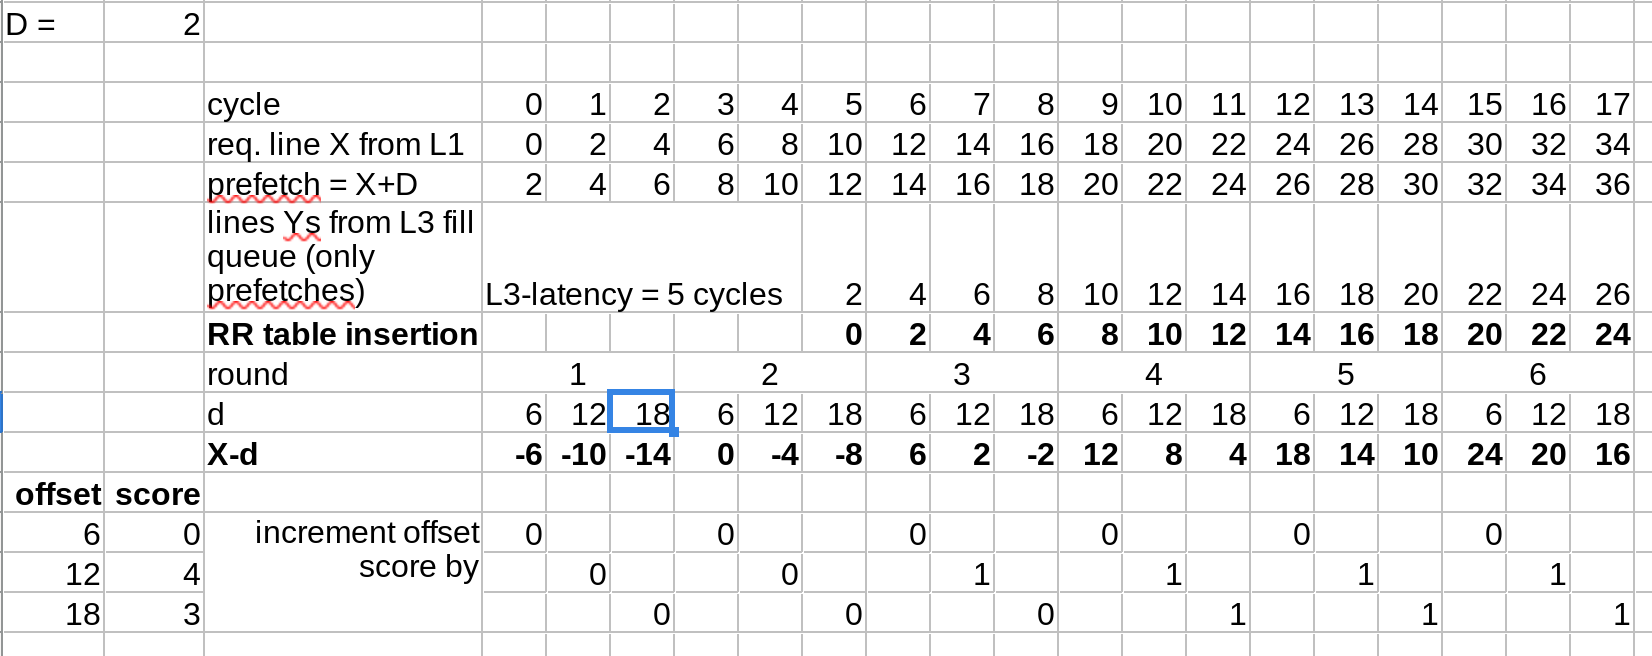
\includegraphics[width=1.0\columnwidth]{figures/example_demonstrating_impact_of_high_latency.png}
    \caption{Example prefetcher execution for a strided pattern and large latency. BO learning favours timely offsets.}
    \label{fig:bo-prefetcher-execution-high-latancy}
\end{figure}

Secondly consider a 'negligible' L3 cache latency of 1 clock cycle, but a more complex access pattern of two interleaved patterns with strides 3 and 4.
The current prefetch offset is $D=2$ again. The offset list contains $d_i = 1,2,3,4,12$.
Figure \ref{fig:bo-prefetcher-execution-interleved-patterns} shows the first 7 rounds of the learning phase.
The score for the offsets 1 and 2 are smaller than for 3 and 4. Which highlights that in at least some rounds these are considered to be a good prefetch offset.
But after some time the prefetch offset 12 is always considered as a good prefetch offset, because it is a multiple of 3 and 4 -- the strides.
Here the algorithm finds the offset that is a multiple of all strides.
\begin{figure}[h]
    \centering
    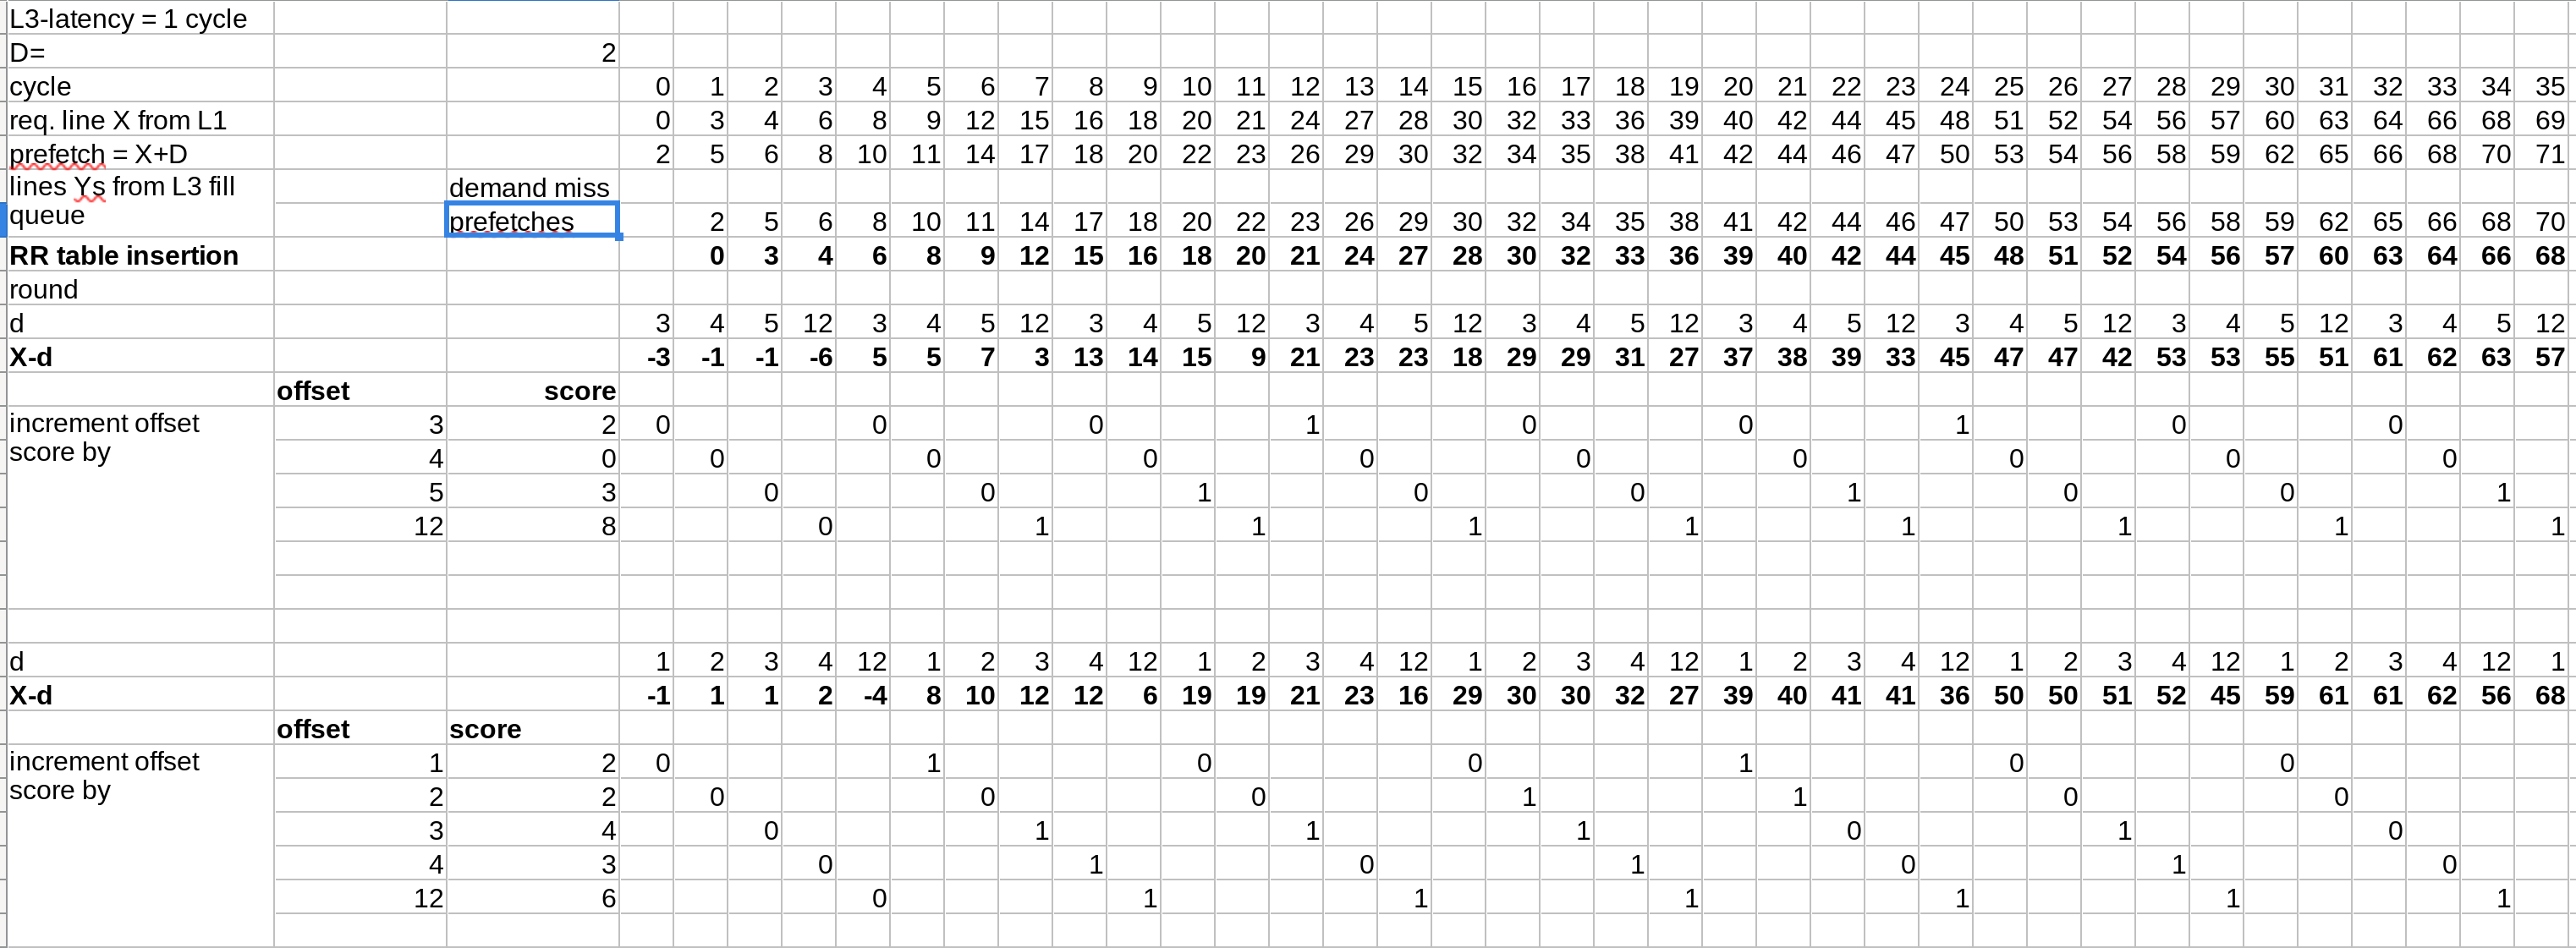
\includegraphics[width=1.0\columnwidth]{figures/example_demonstrating_scoring_multiple_of_both_streams_higher_than_multiples_of_only_one_part.png}
    \caption{Example prefetcher execution for interleaved access patterns. BO learning favours multiple of both strides. (NOTE: only execution for offsets 1,2,3,4,12 (lower part) is relevant)}
    \label{fig:bo-prefetcher-execution-interleved-patterns}
\end{figure}



\end{document}
